
\documentclass[10pt]{book}
%\usepackage{pgfpages}
%\pgfpagesuselayout{4 on 1}[a4paper,border shrink=5mm]
\usepackage{amsfonts}
\usepackage{amssymb}
\usepackage{color}
\usepackage{graphicx}
\usepackage{scrextend}
\usepackage{pifont}
\usepackage{soul}
\usepackage{titlesec}
\usepackage[normalem]{ulem}
\setlength{\parindent}{5mm} % Default is 15pt
\setlength{\parskip}{4mm}
\titleformat{\chapter}[display]  {\large\filcenter}{\MakeUppercase{\chaptertitlename}~\thechapter}{0pt}{\huge}[\vspace{-40pt}]
\renewcommand{\chaptertitlename}{Session}
\usepackage{geometry}
\geometry{
 a5paper,
 % due to the folded nature of my printouts, and the failure to scale the paper correctly
 % the bottom and non-bound margins have extra space. The top and the bound margin
 % are expected to be the specified offsets here.
 bottom=4mm,
 left=2mm,
 right=2mm,
 top=20mm,
 bindingoffset=15mm,
}
\usepackage{fancyhdr}
\fancypagestyle{mainmatter}{
  \fancyhf{}
  \fancyhead[CE]{Session \thechapter}
  \fancyhead[CO]{\leftmark}
  \fancyhead[LE,RO]{\thepage}
}
\newcommand*{\sceneHeadline}[2][]{%
    \noindent\makebox[\linewidth]{#1%
    \textbf{#2}
    \leaders\hrule height \dimexpr.5ex+.2pt\relax depth \dimexpr -.5ex+.2pt\relax \hfill\kern0pt% Right rule
    }
}
\newcommand*{\jumpHeadline}[2][]{%
    \noindent\makebox[\linewidth]{#1%
    \leaders\hrule height \dimexpr1.5ex+0pt\relax depth \dimexpr -.5ex+1pt\relax \hfill% Left rule
    {\MakeUppercase {\large \textbf{#2}}}
    }
}
\newcommand{\subChapterTitle}[2][]{%
  {
\begin{center}
 {\LARGE \textbf{#2} } 
\end{center}
  }
}
\newcommand*{\extraIndent}[2][]{%
  {
   \parskip=0pt
   \begin{flushright}
    \-\hspace{3cm}#2
    \end{flushright}
  }
}
\newcommand{\quotedDialog}[2][]{%
   {
   \parskip=0pt
   #2
   }
}
\newcommand{\deets}[3][]{%
   {
   \parskip=0pt
   
   \noindent\textit{Notes}: #2
   \\
   \noindent\textit{Date}:  ~#3
   }
}
\newcommand{\memoryScene}[2][] {
 {
 \parskip=0pt
  \parindent=0pt
  \leftmargin=5cm
  \begin{addmargin}[3em]{0em}
  ~\\
  #2
  \end{addmargin}
 }
}

%\color[RGB]{204,0,0} % orig color
%$\nsim$ Lackovich $\nsim$
\newcommand{\jayaBrain}[2][]{{\color[RGB]{102,0,0}$\approx$#2$\approx$}}

% $\Rightarrow$Carruthers$\Leftarrow$
%\color[RGB]{230,145,56} %orig color
\newcommand{\hayleyBrain}[2][]{{\color[RGB]{102,65,0}$\rightleftarrows$#2$\leftrightarrows$}}

%\color[RGB]{106,168,79} % orig color
\newcommand{\oliverBrain}[2][]{{\color[RGB]{64,102,48}$\rightarrow$#2$\leftarrow$}}

%$\supset$Signe$\subset$
%\color[RGB]{60,120,216} % orig color
\newcommand{\jonahBrain}[2][]{{\color[RGB]{29,57,102}$\Supset$#2$\Subset$}}

\renewcommand{\contentsname}{Session}
\begin{document}

\begin{center}
~
\vskip 10em
``The world wasn't destroyed. There was no great catastrophe. Nothing in particular went wrong. The trains just stopped running.''

- Nathaniel Ford 5/10/12
\end{center}

\pagebreak


\jumpHeadline{Adam}
\textbf{Character:} Oliver Langdon\\
\textbf{Nickname: }L[a-z]*	\\
\textbf{Class: }Citizen	\\
\textbf{Serial Number: }1195725475	

``While on duty, Oliver slouches and keeps a day's stubble growth on his face.  His mid-brown hair looks to be cut by someone with apathetic scissors.  His uniform conceals the surgical repair of his bad knee, but nothing can hide his lopsided limp.  Though he has a poor complexion and a bad attitude towards authority, he is quite likeable and forms friends quickly - even among those below his social class.  Though he never speaks of Transit Minor, a shadow of past trauma hovers near him, visible to those who are sensitive to such nuances.

When in the company of his peers outside of the Authority, Oliver's posture, outward politeness, and personal upkeep improve dramatically, but his bitterness and anger at those in positions of power still erupt sometimes.''

\vskip 5em

\jumpHeadline{Ion}
\textbf{Character:} Jonah Gemayel (Timon)		\\
\textbf{Class: }National (Franchise)	\\
\textbf{Serial Number:} 4018675308	

`` Dark, mid-length wavy hair, dark eyes.  Usually with a small amount of stubble, neither well-shaven (the mark of the wealthy) nor so long as to be unkempt.  Average height, fairly fit. �He dresses practically, the uniform of the TA being joined by the packs and pragmatic satchels of a street medic.  Jonah appears to be relaxed most of the time, with a cheerful but mild attitude, and a small but constant smile.  That other people tend to see him as friendly but not terribly notable, is a testament to his nearly constant attention to maintain this demeanor at all costs.  The facade rarely cracks.  When it does the tension in his eyes that flickers into view is momentary and so out of place it is easily dismissed.''
 
 \pagebreak
 \jumpHeadline{Rebecca}
\textbf{Character:} Jaya Parvadi	\\
\textbf{Nickname: }Patches	\\
\textbf{Class:} Franchise\\
\textbf{Serial Number:}	1195725475	

``Red rimmed eyes, heavily lidded under heavy brows. A gaunt face atop an equally tall, gaunt form. What little body fat she has is not worn well. Tattoos crawl over her dark skin. They curl below her lips, spot her limbs, and disappear down the cuffs and collar of her worn Transit Authority uniform. Chemical stains are visible on fingers and teeth that flash in grins or grimaces every time she takes another drag on some hand rolled cigarette.''

\vskip 10em

\jumpHeadline{Suko}
\textbf{Character:} Hayley	\\	
\textbf{Class:} Incorporated	\\
\textbf{Serial Number:} 2460124601	

``Appears to be in her late teens at first glance, but is probably in her early 20?s [actual age 23]. Stunningly good looking, Hayley has huge pale blue-grey eyes, a flawless golden complexion and absolutely symmetrical features. Her glossy black hair is cut in a practical short cropped style that only serves to emphasize her elegant bone structure. Her figure is tall, leggy and nicely proportioned. She looks healthy, and only slightly less nourished and well fed than a Citizen. Certainly better than most Indentured. She is toned and fit, and moves gracefully like a dancer. She has excellent posture, always. You have never seen her slouch or sprawl. For those who notice such things, she does not act like someone who is really aware of how their appearance impacts other people. She certainly does not purposely solicit that type of attention.''
\tableofcontents

\pagestyle{mainmatter}
\renewcommand{\chaptermark}[1]{ \markboth{#1}{} }

\setcounter{chapter}{ 0 }
\chapter{\textbf{SAC-09, Intro} }

\subChapterTitle{``PG1 Assemble!''}


\deets{\hl{Missing}\footnote{\textbf{Rebecca S. }These notes were hand written. They have never been recovered. \textsubscript{08/21/15 9:20am}}}{June 7th, 2012}

\textit{\hl{The days pass with a regular, lightless rhythm.}}\footnote{\textbf{Suko T }From first session email 6/6/12
``(4T) Book One: Departure, Episode One: New Station'' \textsubscript{08/25/15 3:39pm}}\textit{ Mess happens like clockwork, PT twice a day on the stretch of concrete called the 'Ready Line'. Sometimes, Morgan watches from the catwalks above where her disgust is hidden in shadow. Tiburon shows you how to fill out the paperwork for the requisition cage and Jari slips Jaya some playing cards one night with her meal. The rest of the days are bounded by the dull grey walls of the barracks, and the faces of your team. Tomorrow, though, Tiburon says to be ready. Tomorrow you're going to New Station. Briefing is at oh-six hundred. Pre-ops to be complete by oh-eight hundred. What the hell are pre-ops?}

The team (Jaya, Oliver and Jonah) rolls out on what was thought to be a normal mission with their new squadmate, Hayley (who appears to be very poorly trained, if at all). That mission turns out to be collecting Victor from a bar located in the Bucket. We bring him in and then find out that we're to take him somewhere else... that turns out to be SAC-09.  We are officially brought into SAC-09 and meet the base personnel for the first time, Morgan, Rook, Jari and the doctor.

 \vspace{\fill}

\begin{flushright}
\textsubscript{last edited by \textbf{Suko T} @ 08/25/15 3:41pm}
% Exported @ 08/26/15 9:13am
\end{flushright}

\setcounter{chapter}{ 1 }
\chapter{\textbf{New Station, Part 2} }




\begin{center}
 {\LARGE \textbf{``His August Person, The Provider Poseidon''} } 
\end{center}




Notes: Suko

Date: June 20, 2012

\noindent\hrulefill





Last session lead-in: After killing Merlin with a well placed headshot, we were told by Angela that ``Poseidon had granted an audience with his august presence.''



We step away from Angela and chat for a while to create a loose plan.  Basically Jonah will do the talking and the rest of us will do our best to shut up.



Angela leads us inside a large building and through a surprisingly clean lobby to an elevator, guarded by two teenage boys.  We ask Angela to accompany us into the elevator.  Despite some misgivings, we step into the elevator and it goes slowly up, while sitar music plays tinnily through the crappy speakers.



Hayley asks Angela about the proper address for Poseidon (His August Person, The Provider Poseidon) and what we could do to make him like us better or at least not dislike us (nothing).  As we step out of the elevator, Hayley asks what Poseidon is to Angela, to which she replies that they work together occasionally.



The elevator opens into a large room, well lit.  There are many women there and several children (infant to about 6 years old).  There are five men on the floor, one by the elevator, the other four by several corridors/exits that branch off of the main room.  They are all standing and have pistols, but they are holstered.



Hayley notices with her Bodyguard training that there are strange packages bolted to the walls with wires coming out of them.  She doesn't report this to the rest of her team.



We go through some double doors at the far end of the room and are in a room with raised platform in it and a bay of windows.  There is a man lounging on a couch on the platform, with a young, very pretty girl beside him who looks at us vacantly.  Jonah's medical training tells him that she's probably hale but there's something wrong with her focus.



They are the only other people in the room besides us and Angela.



Jonah steps forward to address the man and Hayley interrupts him to make sure he knows the proper address.  She bows and addresses Poseidon by the title Angela told her.  Poseidon claps and then Hayley steps back to let Jonah speak.



Jonah starts negotiating with Poseidon, hampered by the fact that he can't actually offer anything of value in return or make any real promises and assurance.  But he appears to make Poseidon at least consider the situation.  



Angela is asked to leave the room when it becomes clear that we will have to be specific about who Poseidon/Trenton is and that we have orders from the TA to bring him home.



While he never directly confirms it, Trenton implies that he is who we are looking for and that he even has some idea of why we are being sent for him.  Certainly more of an idea than we have.  Trenton wants to know where we are stationed and where he is going.  Jonah is cagey and doesn't tell him but Oliver eventually tells Trenton that we are in SAC-09, which causes Trenton to look something up in a book filled with numbers and equations.  Trenton tells us that the trains require particular key sequences to get to certain stations, so if he wanted to, we wouldn't be able to return here via train.



Oliver and Jaya intimidate him into feeling less secure in his cozy little fiefdom, and Jonah uses Social Chameleon to lean on the opening and convince Trenton that it is a good idea to go with us willingly.



Wanting to know who gave us the order to fetch him, we initially tell him Agent Tiburon Rook but then later Oliver describes Agent Morgan who Trenton calls Gerhauser.  This seems to interest him and he appears to know her.  He says she runs in ``strange circles'' but that he hasn't seen her in a while (for obvious reasons).



He eventually agrees to go if we agree to let him bring as many of his family as will fit in the train.



He leaves the room to make arrangements, and we sit around waiting.  Jaya hands a cup to the woman and asks, then orders her to put it away.  The woman, Signe, freaks out.  Jaya backpedals enough that Signe doesn't attack her, and instead Signe stalks away, her posture full of tension.  Hayley, following Jonah's instructions to keep an eye on Signe, follows her.  When Signe asks, Hayley tells her that she was instructed to keep an eye on her.  Not wanting to make things worse, Jonah and Oliver tell Hayley to leave Signe alone.  Jonah scolds Hayley for telling Signe about the order to watch her. 



Trenton returns and discovers that Signe is missing and that we upset her. He gets upset and says he can't leave without her.  Apparently she's got some emotional issue that he's helping her work through, and the last time she freaked out, it took days to find her.



Jaya tells Hayley to look for her, and then amends it to ``to the best of her abilities ascertain where Signe is'' {[}Note by Suko: this was a very smart order change on Rebecca's part- the former order would have had almost totally useless, if potentially funny, results{]}.  Hayley goes out to the women and asks them for information.  Things almost get derailed when Hayley tells the women that Merlin is dead, but eventually one of the women mention that sometimes Signe goes up to the roof.  Hayley and Oliver head up to the roof while Jaya and Jonah go downstairs to ask the guards there if they saw anything.



Oliver uses the scope on his sniper rifle to find Signe who is extremely hard to spot.  She is on the edge of the roof and her eyes go in and out of focus as she seems more or less aware of where she is and what's going on.



Hayley and Oliver eventually talk her down, and Hayley makes Signe a personal promise that Signe will be welcome to go with the rest of Trenton's family and will not be hurt (nor the rest of the family be hurt).  Hayley escorts Signe back downstairs while Oliver lingers behind so that his sniper rifle (initially used to find Signe) won't upset Signe further.



Jaya and Jonah head downstairs to the lobby but don't find Signe.  Jonah finds Angela and talks with her.  He tries to get some information out of her but ends up accidentally feeding her information about the current state of affairs between the Directorate and Anglia {[}refreshing Vigilant{]}.



We all reconvene on Trenton's floor and the leavetaking scene is so heartbreaking that both Hayley and Jonah get flaws of Guilt. It is clear that we are ripping apart a family and a community.



Eventually we get everyone bundled onto the train, much to Tiburon's trepidation.



We stop briefly at DX Station where a diplomatic envoy from Anglia is passing through.  Trains are backed up and being rerouted to accommodate this.



Hayley and Oliver stay in the train car (former due to her promise to Signe and the later due to PTS from his time trapped at DX Station during the war).  Jaya goes with Jonah to investigate what is going on.  She sees the delegates, followed by two extraordinarily beautiful women.  Jaya manages to get herself noticed (senior TA authority) and one of the women comes over to her and smiles and takes her hand.  She thanks Jaya for our hospitality, and then moves on to others in the crowd.



After about 45 minutes, the traffic snarl starts smoothing out and we eventually make it back to SAC-09.


\jumpHeadline{Quotes }

``She smiles slightly but her eyes don't really focus on you.''

``So she IS like the girls I used to date!''

\extraIndent{ - Nate (describing Signe's reaction to Oliver) and Adam}



``I'm not magic.  Well actually I kind of am.''

\extraIndent{- Trenton (Poseidon)}



``Yeah you stay here...I'll go upstairs and, uh, cover our tracks.''

\extraIndent{- Jaya, to Jonah}


\vspace{\fill}

\begin{flushright}
\textsubscript{last edited by \textbf{Suko T} @ 05/29/15 11:01pm}
% Exported @ 08/22/15 12:54pm
\end{flushright}

\setcounter{chapter}{ 2 }
\chapter{\textbf{Cardoza Station, Part 1} }



\subChapterTitle{``Drowning in Pudding''} 

\deets{Ion}{July 12, 2012}



\jumpHeadline{ Shore Leave! } 


\sceneHeadline{Shore Leave: Jaya }

Padme (Jaya's sister)'s son Simon has been sent to the mines.  Padme doesn't seem too concerned but Jaya wants to get him back.  Padme has recently given birth to Micah, and tattoos with the kid on her lap.  Both sisters are openly disappointed that it's another son.  Banter ensues, with the sisters cheerfully insulting each other, Jaya telling Padme ``you are great at tattooing but not good with kids'', and Padme asking Jaya why she doesn't have kids yet.  Jaya wants to get Simon back but Padme doesn't see the point in spending money on him.  Jaya seems to care about having ``a good kid'' not be wasted, but Padme believes she's just doing this to avoid having children of her own.  Jaya denies it vehemently ... so it must be true.


\sceneHeadline{Shore Leave: Hayley }

Hayley is in the gym.  She was gone from her ``main contract'' for several days on the last mission.  Her employer is disgruntled about her absence.  Hayley points out that she can't just leave.  She's at the bottom of the social structure, which she believes is very strange.  She doesn't understand the military ranks, and believes that they violate the natural order (by Citizens being lower rank than Nationals for instance).  ``Power seems to be expressed by belittling other people''.  This her employer feels is at least right and proper: ``Some people should be put in their place''.  Now we get to the meat of things: her employer wants to know exactly what Hayley's patrol squad has been doing.  Hayley explains about the new station and the mission to find (Trenton) and re-open the station.  She gives her a crudely drawn map of the area around New Station that you could see from Trenton's building's rooftop.  Her employer finds this somewhat comprehensible.  Hayley tries to ask about the codes that control the trains but her employer doesn't find it believable that trains are controlled by codes.  Hayley did write what numbers she could see from seeing Trenton's book, but they are not complete or comprehensible, being mostly just random numbers and squiggles since she doesn't know mathematical symbols or formulae. Gillian believes she can find someone who knows how to interpret them {[}Suko's note: But it will be next to useless since they are the equivalent of seeing half of a page of a 100 page mathematical expression, while looking at it upside down{]}.  Hayley says there is more information in her reports that were submitted, presumably separately.  Her employer is somewhat insistent that Hayley come back soon.  DeVries (a Citizen that she dislikes) is becoming a real problem for her.  Hayley doesn't see an easy way to get sent back from the TA other than getting severely injured... which she expresses a preference for avoiding since it counters her contract holder's instructions to avoid getting killed.  They agree to have her uniform re-fitted by the house seamstress (!).


\sceneHeadline{Shore Leave: Oliver }

Oliver is in his room trying to get undressed and wind down.  His mother comes in to tell him something, but sees his war wound and gets suddenly withdrawn (embarrassed?  unclear).  They make awkward small talk.  He complains about the rest of his team, how they are incompetent and don't know what they are doing.  He's not happy that he is reporting to a Franchise person.  She wants him to meet with people who can further his career and get out of his niche.  Mostly it's uncomfortably oblique, until Oliver directly asks if she can put him in touch with someone.  Ironically she wanted to do just that, but they are interrupted by the dinner bell, and the conversation goes unsaid.


\sceneHeadline{Shore Leave: Jonah }

Jonah is working with his cover identity.  He is being asked by his bandage supplier (one of his reliable suppliers) to get some application forms for the medic academy for the supplier's son (Mika).  Jonah promises to look into getting the form.  He is pretty sure he can't get the form and gets the run around at the academy, but he tries.  He talks up a young man at a desk and finds out that the best way is to get a Citizen to get an appointment with a dean who can get you an application form.  This being infeasible, to put it mildly, Jonah then talks to one of his street medic friends to see if he wants an apprentice.  The friend says he'll consider it and for Jonah to set up some kind of meeting.  Jonah goes back to his bandage supplier and convinces him that getting into the academy is tricky but that his son's odds are improved by having experience, so he should consider getting him apprenticed.



\jumpHeadline{Session } 



Oliver at the medic's.  They get along \textit{fabulously}, the doctor taking blood samples and Oliver giving her a hard time for every procedure.  She asks Oliver about the leg which he tries to avoid talking about but she presses on telling him the missions need everyone to be in good shape.  {[}Out of nowhere an out-of-game cat bolts across the hall, leaving all characters strangely confused{]}.  The doctor prescribes that Oliver go down twice a week to the cistern and swim.  Oliver claims that there are deep bone injuries that can't be fixed by swimming which he's already had a doctor look at.  She calls his bluff saying that that's not his actual problem.  The leg can be fixed eventually but that's not his issue, and does he want her to spell it out?  Oliver quickly retreats without admitting anything saying the exercise will be great.  He calls her ``ma'am'' and winks at her on the way out.


\memoryScene{
Notes:

- The leg can be fixed?

- The doctor is Morgan's sister.
}


Jaya gets called by the intercom and folds at cards.  She's happy, so she gets Oliver's last name totally wrong.  The room she goes to has empty tanks (cisterns?) ... and Morgan.  Jaya saunters in and straightens up abruptly when she sees Morgan.  Morgan tells her she finds Jaya's (or the team's?  It was unclear) performance mediocre.  Jaya tries to claim that the team's performance is basically par.  Morgan says that she was under constraints for choosing who would be on the team, constraints which in this case were apparently mostly medical.   She adds that the team with some work can be adequate.  She says that ``we'' (the Directorate?) have enemies.  Jaya says ``Nicklepan'' but Morgan corrects her saying that Anglia is actually who she is referring to.  She expects that the team can be made better but expects Jaya to rise to the cause.   Jaya is clearly intimidated by the idea but says she can do it and stammers her way out.


\memoryScene{
Notes:

- The constraints for team selection were medical.  (Medical???)
}


Trenton comes to the barracks.  Hayley opens the door.  When Jaya says ``close the door'' Hayley shuts it in his face.  Trenton comments on Hayley's literalness (and pliability?).  He invites Jonah to follow him.  They walk out to a door that says ``machine shop'' saying he needs a ``pair of steady hands''.  Jonah notes that he is pleased they let him walk around, and inquires as to where Trenton actually is most of the time, to which Trenton replies obliquely: ``around''.  They banter about Morgan's sex life (scary!) then Trenton tells Jonah that they are hooking radios to the trains.  Trenton shows him how they work, and Jonah is (unusually) visibly impressed.  Trenton explains a little bit about them.  Trenton then asks Jonah if he knows where they are.  Jonah replies that he tries not to ask questions he won't get answers to.  Trenton continues on conspiratorially that he thinks even the DIrectorate doesn't know where they all are because Morgan doesn't want them to know.  He asks if Jonah has considered that SAC-9 means there are at least 8 other SACs.  Jonah says he doesn't even know what a SAC is.  After Trenton explains he says these are places the TA must've rediscovered recently, but how long ago? Trenton then points out a noise on the wall that he can't identify.  Where IS the SAC?  As they part Jonah comments that he's pleased Trenton isn't locked up some place.  Trenton grins and says it's not \textit{him} who's locked up with \textit{them}.



(While he's gone Jaya and Oliver try to explain Hayley that Trenton is trying to get into her pants.  They try to teach her how to say ``No''.  The operation cannot be called a success.)


\memoryScene{
Notes:

- The radios are from Cydonia.

- ``SAC'' means ``Stand-Alone Complex.''
}


Hayley gets summoned somewhere by the guards.   She follows them down the hall, which is  followed by an hour(?) she has no memory of.  When she wakes up she's drowning in a container of purplish-bluish liquid sealed up. There's no breathable air and after a concerted effort to right herself and find a breathable point Hayley starts to panic.  She starts to punch the top to try and get out.  She breaks her hand, sees a dark red in the liquid, blond hair swirling around her head and then passes out.



Hayley wakes up in a bed, a medic? standing over her with a badge that says ``Swan''.  She asks if she had a nightmare and he says no but she did very well.  It was a test, and, when she asks, he has authorization from Dr. Gerhauser who was pleased with the result.



Hayley seems very confused about who Dr. Gerhauser is asking for authorization if it's her contract holder or ``the Agent'' (meaning Morgan).  The medic doesn't really answer the question but tries to make sure Hayley is ok before he sends her back.  Hayley asks if she is the only one who has to undergo the tests and the agent replies that so far yes, but the others will be doing them too.



Hayley is gone for 8 hours.  She comes back in the night.  Oliver wakes up and asks her where she is.  (Jonah listens in without saying anything or showing he's awake.)  She tells him, and when she gets to the part about almost dying, he gets angry and wakes up Jaya and all three interrogate Hayley about what happened.  (Jaya jumps out of bed and salutes, sleepily demanding that everyone be presentable.)  No one is ok with the prospect of being drowned as part of testing.  Jaya and Oliver quarrel about whether they should go back to sleep.  Eventually Oliver says he is going ``swimming'' which makes Jaya and Jonah snort and say ``good one''.  When Oliver leaves with his swim trunks and towel Hayley asks if she can go, and the others stop her assuming Oliver is just jerking her around and wanting some private time.  (The idea of swimming as a non-Citizen isn't just decadent but actively insane, since pools of water are so dangerous.)


\memoryScene{
Notes:

- Agent Morgan Gerhauser's sister is the doctor.
}


Oliver goes down to the cistern to swim.  It's reasonably well lit and deep.  It is \textit{cold} but very relaxing and comforting.  He finds it's pleasant to have the pressure off the leg.   After 15-20 minutes he gets too cold and gets out.  He then goes to practice shooting (though there isn't really a range).  Just as he is coming back the alarms go off.



The red alarms flash, the klaxons shout.  Everyone gets ready to leave.  Oliver shows up as the others are leaving.  There is some confusion as Oliver and Jonah go back to get Oliver's equipment despite Jaya insisting they go as fast as possible.  When they show up at the line-up Morgan isn't obviously more displeased than usual.  She walks towards the train saying she'll brief the squad on the way.  She asks if they are familiar with the name DeVries, noting that they won't have the pleasure of meeting him since he's dead.  {[}Note: Hayley's employer mentioned DeVries being a problem in session 2....{]}  The TA came into the possession of a letter written by DeVries that indicates a rogue Citizen has an explosive device.  The mission is to pursue the man to Cardoza and get back the device and apprehend him before he ... blows up Anglia.   (Jaya gets a clarification about whether the man needs to be alive after apprehensions.)  Then she grits her teeth at Jaya and says ``Impress me'' as she did before.  As the team boards the train Morgan seems unusually tense, like she's doing something distasteful yet also a little eager.



On the way to Cardoza the train goes faster than anyone has ever experienced.  It then decelerates rapidly inducing nausea and causing most of the team to stumble and or fall.

The address is that of Citizen Cyril Magnin.  Oliver knows Cyril Magnin isn't terribly popular, with a reputation as a troublemaker.  He is pro-Directorate and isolationist, believing the Directorate should not have gone to war with Nicklepan or be allied with Anglia.   He is married ,very wealthy and has stakes in a number of companies.  Despite his reputation he has enough influence that people invite him everywhere.



When the doors open there are people waiting with bags looking put out that the train was so abrupt.  There is an altercation between a man who complains about schedules and Jaya throwing TA authority around.  Jonah suggests being stealthy.  Oliver extracts them and they end up on the road.  Most of the traffic is servants.  Oliver suggests hiring a carriage.  (Which they do with Oliver's parent's tab.)  When they arrive Jonah notices a crowd of TA agents directing people.  Jonah and Hayley go to ask them what's going on while Jaya and Oliver go to case Magnin's house.  Jaya and Oliver debate tactics and conclude that Oliver will get on a roof to give him a shot.



Jonah learns the other TA group is \textit{also} looking for Cyril Magnin.  He convinces them he got directions which send them in the wrong direction.  The four constables then debate how to get into Cyril Magnin's mansion.  They fail to take advantage of the servants entering the building.  After discarding several plans for pretending to be servants or pretending to be there to look for something, they decide they are out of time.  Jaya and Jonah head for the front door to claim they are looking for stolen jewelry.



\jumpHeadline{Challenges } 

{
\parskip=0pt

- Knowing who Cyril Magnin is: 1.  \textit{Citizen: 1} (Oliver).  Matched.

- Get to Magnin's place fast: 1.  \textit{Family Money: 1} (Oliver), \textit{Streetwise: 1} (Jonah). Overcome: 1 VP (Oliver)

- Notice the crowd of TA agents giving directions: 2.  \textit{Vigilant: 2} (Jonah).  Matched.

- Deceive other TAs looking for Cyril Magnin to go the wrong way: 2.  \textit{Social Chameleon: 2} (Jonah). Overcome: 2 VP (Jonah)

- Prevent crowd walking by from overhearing us talking about bombs: 1: \textit{Concealment: 1} (Jonah), \textit{Senior Constable: 1} (Jaya).  Overcome: 1 VP (Jaya).
}


\jumpHeadline {Quotes }  



``Just shut up and finish the `Fuck' ok?''

\extraIndent{- Jaya, getting a tattoo from Padme that says ``Don't Fuck with the TA''.}



``I'm sure it will be alright as long as I can get off on the right foot. ... uh.'' 

\extraIndent{- Oliver, to his mother.  (Oliver's right leg is the injured one.)}


\quotedDialog{
Jaya: ``Where the \textit{fuck} is Langdon?'' (She gets his name right)

Jonah (making fun of her): ``Who's 'Langdon'?''

Hayley: ``Maybe he drowned?''
}


``Senior Constable, someone once told me there are only two pains in life: the pain of discipline and the pain of regret.  I'm going to see that you have no regrets.''

\extraIndent{- Morgan, to Jaya}


\quotedDialog{
``Yes ma'am sir! I can maintain team discipline, even when Johnson {[}Oliver{]}...''

``Shut up and show me.''
}
\extraIndent{- Jaya and Morgan}



``I didn't know her name.  I don't usually ask any more.''

\extraIndent{- Hayley}



``You know, I don't think she said `No'.''

\extraIndent{- Jonah, to Jaya and Oliver, after Hayley is gone for hours}


\quotedDialog{
``Do you know what day it is?''

``I think it's Thursday.''

``And who is the holder of your contract?''

``I'm sure it was in the forms.''
}
\extraIndent{- Swan, trying to figure out if Hayley is ok, and Hayley}


\quotedDialog{
``Are you ok?  Where were you?''

``They were putting me through a test.''

``What kind of test?''

``Well I think they tried to kill me.''

``WHAT?!?''
}
\extraIndent{- Oliver and Hayley}


\quotedDialog{
``What?  How?''``I think they tried to drown me in pudding.''

``What were they testing!?!''

``That's a good question.  I should have thought to ask.''
}
\extraIndent{- Oliver and Hayley}



``Maybe it was a test of lung capacity.  Or blood oxygenation.  I'm really good at that!''

\extraIndent{- Hayley, grinning widely}


\vspace{\fill}

\begin{flushright}
\textsubscript{last edited by \textbf{Nathaniel Ford} @ 05/07/15 4:28pm}
% Exported @ 08/22/15 12:58pm
\end{flushright}

\setcounter{chapter}{ 3 }
\chapter{\textbf{Cardoza Station, Part 2} }


\subChapterTitle{``Ire of the Orc of Anglia''} 

\deets{Rebecca}{July 24, 2012}

\noindent\hrulefill





Other Dudes:  Citizen Cyril Magnin: He is pro-Directorate and isolationist, believes Directorate should not have gone to war with Nicklepan or be allied with Anglia.



Our Dudes: Oliver Langdon, Jonah Gemayel, Jaya Parvadi, Hayley.



\begin{itemize}
\item OMG - The doorbell is about to be rung ... RANG! Jonah nearly flubs it, but Jaya \& Jonah bully themselves through the front door.
\item Oliver, lookin' for power cables. Spots the 3B Trunk line on the north side of this building here and a 130 power gauge coupling there.  TA business to investigate them.  Talks to a burned face man working for the power repair about how to find them.  This leads Oliver to climbing a fire escape.  As he glances over his shoulder and spots buddy Roger watching him.  Oliver flashes the TA patch and all is cool. 
\item TA Team 6 approaches!   Jaya and Hayley and Oliver chat briefly on the walkie-talkie.  Hayley is ordered to avoid detection and to enter the premises. 
\item Jonah interviews Ruth (the maid) an odd lady.  (Incorporated, MMDVI company, whole life.) Talk about recent guests of Cyril Magnin's.  A recent dinner party was composed of DeVries, John Bay (and escort), Lady Potter (and escort), and Sutter (unescorted).  Ruth is usually the only person there, but for parties they hire extra help.  There was a new staff member, Rowan.
\item Hayley sees some locked doors and trash cans.  She *totally* ninja climbs up the wall all quiet like!  She is not spotted as TA Team 6 passes by the alley.  Whoo! 
\item Oliver is on the roof, peeping in people's windows with his rifle.  He sees a dude running across the rooftops toward Cyril Magnin's house!  He tries to radio in.
\item Jaya thinks creeping up stairs is super easy... turns out not so much.  Steps on squeaky floorboard, swears, and has a gun pulled on her!   {[}\textbf{Flaw 1: Flat Footed (Jaya)}{]} {[}\textit{5 threat tokens enter pool}.{]}   Him: ``Don't move!''  Jaya: ``TRANSIT AUTHORITY! DROP THE GUN!''    Gunfire is exchanged! It's totally intense!  Jaya gets a dramatic flesh wound and that just spurs her on- she sprints down the hall and bludgeons the fellow.  YEAH!  Oops! Gotta' reload the gun.... 
\item Hayley tumbles into the house and onto Jonah.  Oops!   They collapse in a heap.
\item \hl{The Orc of Anglia! introduced!  {[}\textit{10 threat tokens enter pool}.{]} }\footnote{\textbf{Nathaniel Ford }So few tokens. \textsubscript{01/07/15 10:45am}} Oliver tries to shoot the roof rat and gets a solid shot and knocks 'im back on a deck!  {[}\textbf{Flaw 3: Ire of the Orc of Anglia (Oliver)}{]}. Buuuuut there was body armour...  Oh shit! It turns out that it was the same guy on the street that gave him directions! Burn Face Man!  In retaliation Burn Face Man chucks a grenade at him - dramatic shit goes down!  KAPOW! EXPLODE! 
\item Injured bodyguard/thug tries to knife Jonah!  Jonah gets a leg wound but Hayley stomps on bad man's leg to deflect most of the blow.  Ouch!  {[}\textbf{Flaw 1: Leg wound (Jonah)}{]}.
\item Jaya kicks down the door and she and Hayley run through the room.  They see a secret stairway that had been hidden behind a bookshelf and head straight for it.  Jonah follows at a slower pace, hampered by his wounded leg.   He pauses long enough to give the room a quick once over and steals some books/papers covered with notations and equations on his way through the room.  
\item Oliver, still outside, starts firing wildly at Burn Face Man.  This is ineffective and attracts Team 6's attention.  They shoot at him \& the Orc for a bit.  Oliver shouts out something effective and military like (\textit{Reputation: Veteran}) and convinces them to shoot the other dood. 
\item Jaya and Hayley reach the bottom of the stairs where there is a steel door.  Hayley flings herself at the door and batters it open, earning herself a {[}\textbf{Flaw 1: Torn shoulder ligament (Hayley)}{]}.  They run for a while down an old tunnel, following the footsteps of their quarry.  
\item Oliver fails to save some folks (2 TA agents and Ruth the maid) from being shot by the Orc because his gun jams (shit happens) {[}\textit{Refresh: Sniper Rifle}{]}.
\item Jaya and Hayley run.  There's another door, but they don't let that stop them.  Jaya orders Hayley to open the door - it's effective! (and painful for one of them).  What's a wrenched back when you're in hot pursuit?  {[}\textbf{Flaw 1: Torn shoulder ligament -\textgreater  Flaw 2: Strained back (Hayley)}{]}  They run some more!  Through some... sand?  Odd terrain?  It is grey and soft like snow (but not cold) and crunches slightly underfoot.
\item Orc goes through the skylight, some Team 6 dudes follow him into the building. Oliver chats with Jonah about the weather.  He bugs out of his crow's nest and heads into the building.
\item Jonah goes through the door that Hayley and Jaya just busted through...  but is a little surprised by the ``Dead People Here'' sigil on the door.  It is a sigil that is often found on gravestones for the rare time that people are buried.  It means ``Primus''?  So distracting!  He is not so distracted he doesn't take a small sample of the odd substance they are running through. 
\item Eshkani is fairly seriously hurt, with a gaping gut wound.  Oliver just breezes by him ``Buck up, Eshkani, it's not so bad!'' -- ``Fuck you, Brown Bagger!'' he says back.  He seems furious that he's being left behind but Oliver is hardened to this sort of thing and doesn't have time to help.
\item Jaya shoots the running person!  But unfortunately he shoots back. Bloody times... Jaya gets a {[}\textbf{Flaw 2: Head wound (Jaya)}{]}.  Hayley just strains herself *even more* {[}\textbf{Flaw 2: Strained back -\textgreater  Flaw 3: Slipped disc (Hayley)}{]}.
\item Oliver is in the house -- the house of BLOOD!  Sees ``Plain Jane'' on the stairs.  ``Useless'' Oliver mutters after the wounded woman gives no intel.   He creeps up the steps...  Rupley is dead up the steps, hand on his throat.  The house is a mess!  Decker is at the top of the secret stairway... he's still alive, but is kinda froze up.  ``My whole squad is down there'', Oliver says.  ``Your whole squad is dead!'' replies Decker.  ``Not them too!'' says Oliver mostly to himself.  Down the stairs he goes! bum Bum BUM!!
\item Jonah gives Jaya drugs and a really big bandaid.  She feels awesome {[}\textbf{Flaw 2: Head wound -\textgreater  Flaw 1: Head wound (Jaya)}{]}.  Hayley starts crying because he's getting away!  Jonah isn't as effective with her, grumbles about being out of stims....
\item Oliver slinks through the dark tunnels...  His radio crackles with Jaya's voice ``Longjohn! ... Train!  ...''  He turns off the the radio, looks around, and turns it back on: ``How. Do. I. Find. You?''  Then there's a raspy voice down the tunnel  ``I'm right here''.  This is Not Good.  Oliver drops to the ground (switches off the radio and flashlight) and starts to army crawl towards the voice.  Mr. Orc chuckles softly. Oliver inches towards the wall... he thinks. ``Where's he going?'' asks the Orc.  Oliver declines to respond, not wanting to give away his position.  After a moment the voice says ``Ah well...  I'm going to make this long and painful.  You have 60 seconds.'' Oliver hears something thud to the ground and sees slight ripples in the water.  There's some ominous beeping.  He gets the hell out of there -- and manages to stagger through the door that he just came out of before the bomb goes off.  
\item Cyril is headed toward a train station, we can hear a train arriving.  We are on the tracks, and can't see anything that is happening on the train platform (and vice versa).  Jaya runs off nearly on her own after Cyril.  Jonah gets Hayley to her feet but she staggers and trips and can't make it onto the train before it leaves.  Jonah makes it onto the train.
\item Jaya and Jonah confront Cyril, who is at the train's front driving it faster.  He has a small box (mechanical device) slung around his neck and is holding a cylindrical steel device.  Jaya tell him to surrender and give up his bomb.  Cyril laughs at them and mocks their ignorance.  There is no bomb he says.  They used ``bomb'' as a way of talking about what they (they?) really have, which is a ... ``camera'' (whatever that is).  They were going to cause massive change, very quickly, like a bomb.  Cyril rants for some time about how the device will show the ``truth about Anglia, not the 'proxy Anglia', the 'real Anglia'''.  Which is not the place where we think everyone is being sent.  Jonah, morbidly curious, tries to find out what ``real Anglia'' means, and learns only that Cyril thinks the Anglia is keeping ``our people'' prisoner in the real Anglia.  Jonah is confused by this and thinks Cyril is working for Anglia, which Cyril denies furiously.  Jonah tries, unsuccessfully,  to convince him that the team also has a bomb which will blow up if they can't stop him.  {[}\textbf{Flaw 1: Burning Curiosity (Jonah)}{]}  Jaya distracts Cyril.   Jonah mans up and shoots Cyril.  Cyril attempts to slam the cylindrical device to the ground but Jaya throws her baton at Cyril and prevents him from doing that.  She knocks it out of his hand, and while he scrambles to get it, Jonah tackles him and zipties him. Jaya slows the train down but not in time for Jonah to treat Cyril and he bleeds out.   Jonah passes the cylindrical device to Jaya and says ``here is the bomb''.  Jonah is an ASS and he steals the ``camera'' portion of the devices, and Jaya doesn't notice although she senses something is up.  The end.  Mission successful!
\item Debriefing!  Jaya has a bandaged head and Hayley has a sexy steel corset.  Everyone gathers in the ops room the next day.    Morgan shows us pictures of Rupley, Ruth, Cyril Magnin and the bodyguard.  ``4 dead'' she says.  She shows us pictures of two more TA agents, Eshkani and ``Plain Jane'' Lackovich and adds, ``and 2 wounded''.  She shows us more slides with numbers.  ``And considerable damages and delays to the trains due to your actions.''  She grudgingly concedes that the mission was successful, but she says it was ``loud''.  
\item Oliver reports the person whom we know OOC as the Orc of Anglia.  Turns out the guy has worked for Anglia 10 years ago!  His face in the photo Morgan displays is very badly burned.  Buuuuurn victim, Krueger style.  Oliver thinks it is the same guy, although it was hard to tell as he had a pitmask on when Oliver met him.  The Orc does dirty work for Anglia and is very skilled. Don't tangle with him!
\item Oliver challenges Morgan about the lack of accurate information and the claim that the mission was ``loud''.  He not so politely points out that keeping it quiet when the mission out was rushed there was a rival TA group that we weren't coordinated with (this seems to particularly anger Oliver), and a random unstoppable goon out of nowhere was also running interference.  {[}Note: Oliver doesn't explicitly say that most of the deaths weren't because of our team.  Actually nearly all of them were the Orc.  We only got Cyril and his bodyguard.{]}  {[}Adam's note: Oliver was basically saying, three groups were here with roughly the same objective and they mostly ended up killing and wounding each other due to lack of communication/coordination.{]}
\item OMG, Oliver just walked out on Morgan! *That's* going to go well...  
\item Jonah asks about the device and whether it was the bomb.  Turns out it is a beacon (which all trains have apparently).  It was not a bomb.  Morgan lectures us that she does not have unlimited resources and that she has to go with what she has.  She admits that she doesn't always have very good information.  She also says that, in the future, we may get more autonomy over how we run our missions.  This is the first sign she's given our group that she has any confidence in us at all.
\item Jaya starts talking to Morgan about why the other TA patrol group was there and how to prevent that in the future.  Jonah interrupts her which earns him a dressing down from Jaya later on.  Morgan says that the other patrol group was sent by a senator.
\item Morgan mentions volunteering for some experimental research-y... stuff.  She directs this to Jaya and Jonah saying she assumes Oliver won't want to, which she seems to think is a shame.  She doesn't include Hayley, presumably because she specifically states that the volunteering is for those who ``are legally able'', which as an Incorporated, Hayley is not.
\end{itemize}



BTW - Mention something about buying skills?   Nate did! It's awesome! Kinda' like 2 for 1!



{[}Rules modification: All point spent on skills will be matched by equal points for the group stash.  This allows us to grow the common pool of useful devices and perks, and helps compensate for the pain point of being separated and being out of skills.{]}



\underline{  {\LARGE Challenges }  }



- Notice challenges: 1x3.  Failed.

- Let Us IN!: 2.  \textit{Grim Visage: 2} (Jaya).  Matched. 

- Find some power cable locations: 2.  \textit{Outgoing: 2} (Oliver). Matched. 

- Not be tattled on by Roger: 1.  \textit{TA Uniform: 1} (Oliver). Matched.

- Noise Detection Challenge: 1. Failed.

- Ninja window climb: 3.  \textit{Dancer: 1 }(Hayley)\textit{, Uniform: 1} (Hayley)\textit{, Athletics: 2 }(Hayley). Matched.

- Notice challenge: 1.  \textit{Sniper rifle: 2} (Oliver). \textbf{ {\color[RGB]{0,0,255}Overcome: 1 VP (Oliver).} }

- Creeping challenge!: 2.  \textbf{ {\color[RGB]{255,0,0}Flaw: Flat Footed: -1 (Jaya). } }Failed.

- Bodyguard Man!: 3.  \textit{Adrenaline Junkie: 1} (Jaya)\textit{, Truncheon: 1} (Jaya)\textit{, Sidearms: 2} (Jaya). \textbf{ {\color[RGB]{0,0,255}Overcome: 3 VP (Jaya).} }

- Shoot the roof rat!: 3.  \textit{Crackshot: 3} (Oliver), \textbf{ {\color[RGB]{255,0,0}Flaw: Ire of the Orc of Anglia: -3 (Oliver). } }\textbf{ {\color[RGB]{0,0,255}Overcome: 3 VP (Oliver).} }

- Grenade headed your way!: 2.  \textit{Hardened: 2} (Oliver). Matched.

- Knife in the gut from a wounded man!: 2.  \textit{Bodyguard: 1} (Hayley), \textbf{ {\color[RGB]{255,0,0}Flaw: Knife wound: -1 (Jonah)} }. Matched. 

- Kick down the door all dramatic like!: 1. \textit{Outfit: 1} (Jaya). Matched.

- Shoot the other dude!: 2.  \textit{Veteran: 2} (Oliver). Matched. 

- Open the damn door: 1.  \textbf{ {\color[RGB]{255,0,0}Flaw: Torn shoulder ligament: -1 (Hayley)} }. Matched. 

- Open the other door!: 2.  \textit{Conditioning: 2} (Hayley). Matched. 

- Where are you, Jonah?: 2.  Failed.

- What's that sigil there?: 1. \textit{Street Medic: 2} (Jonah). \textbf{ {\color[RGB]{0,0,255}Overcome: 1 VP (Jonah).} }

- Run faster!: 1 x 2.  \textit{Dancer: 1} (Hayley), \textbf{ {\color[RGB]{255,0,0}Flaw: Torn shoulder ligament: 1 (Hayley)} } -\textgreater  \textbf{ {\color[RGB]{255,0,0}Flaw: Strained back: -2 (Hayley)} }, \textit{Team Leader: 1} (Jaya). Matched.

- Hit the moving target!: 3.  \textit{Sidearms: 3} (Jaya). Matched. 

- Don't get hit!: 3.  \textbf{ {\color[RGB]{255,0,0}Flaw: Strained back: 2 (Hayley)} } -\textgreater  \textbf{ {\color[RGB]{255,0,0}Flaw: Slipped disk (Hayley)} },  \textbf{ {\color[RGB]{255,0,0}Flaw: Fucked up face: 2 (Jaya)} }. Matched. 

- Escape the bomb!: 2.  \textit{Arm Strength: 1} (Oliver).  Failed.

- Shooting Cyril Magnin and preventing him from setting off the ``bomb'': 2. \textit{Vigilant: 2} (Jonah), \textit{Small Arms: 1} (Jonah), \textbf{ {\color[RGB]{255,0,0} Flaw: Burning curiosity: -1 (Jonah)} }.  \textbf{ {\color[RGB]{0,0,255}Overcome: 2 VP (Jonah)} }\textbf{.}

- Don't blow up the maybe bomb?: 3.  \textit{Truncheon: 1} (Jaya). Failed. 

- Don't let Jonah steal TA evidence: 1.  \textit{No appropriate skill} (Jaya).  Failed.



\underline{  {\LARGE Refreshes }  }



- Jonah acted retarded at the front gate - refreshes Social Chameleon.

- Oliver meets his buddy Roger - refreshes Citizen.

- Hayley creates a pile of constables in the hallway - refreshes Dancer.

- Jaya reloads the gun - refreshes Sidearms.

- Oliver fires wildly at the building - refreshes Crackshot.

- Oliver fails to shoot the Orc due to a gun jamming - refreshes Sniper Rifle.

- Jonah is confused about where he is - refreshes Streetwise.

- Jonah is distracted by all the dead people dust - refreshes Medic.

- Oliver says something jerk-face to the injured guy - refreshes Veteran. (or was it Hardened?)

- Hayley starts crying! - refreshes Conditioned.

- Jonah fails to help Hayley the first time - refreshes Medic.

- Jaya fumbles with the truncheon - refresh Truncheon. 

- Hayley trips and stumbles on the way to the train - refreshes Athletic.



\underline{  {\LARGE Quotes }  }



``Agent! Morgan! Agent! Morgan!''

\extraIndent{- Running mantra}



``Oh he looks like a thug?  Why didn't you say so?  It's okay then.''

\extraIndent{- Rebecca, relieved to have someone it's clearly okay to beat up.
}

\quotedDialog{
``You get to the door before he can lock it''

``Good, because I only had two shoulders''
}
\extraIndent{- Nate and Suko, referring to Hayley's accumulating injuries going through the last two doors.}


\vspace{\fill}

\begin{flushright}
\textsubscript{last edited by \textbf{Nathaniel Ford} @ 05/07/15 4:28pm}
% Exported @ 08/22/15 1:10pm
\end{flushright}

\setcounter{chapter}{ 4 }
\chapter{\textbf{SAC-09, Interlude} }




\subChapterTitle{``Shore Leave''} 

\deets{Suko}{August 13th, 2012}



So.  Many.  Words.



\noindent\hrulefill





We purchase some communal assets, spending 16 points.

{
\parskip=0pt

\textit{Equipment} \textbf{Dispensary }(2): Stocked with first aid kits, painkillers, bandages, antiseptic, cleaning alcohol and basic medications along with handy satchels and pouches to carry such, this is located in a corner of the Requisition cage.

\begin{itemize}
\item \textit{Outfit} \textbf{Medkit} (1): A bundle of bandages, one-use painkillers and antiseptic ointments, this pouch attaches to the leg of a Transit Authority Uniform and is useful for a number of light to medium medical emergencies.
\end{itemize}



\textit{Equipment} \textbf{Radio Network }(2)

\begin{itemize}
\item \textit{Equipment} \textbf{Hush Radio} (1)
\end{itemize}



\textit{Equipment} \textbf{Closet }(1)

\begin{itemize}
\item \textit{Outfit} \textbf{Urban Camouflage} (1)
\end{itemize}



\textit{Equipment} \textbf{Armory }(1)

\begin{itemize}
\item \textit{Weapon} \textbf{Rifle} (1)
\end{itemize}

}


\newpage
\jumpHeadline{SAC-09 } 



After the last session Tiburon and Morgan take us to the Transit Authority HQ where we are subjected to a bit of cross examination about Cardoza.  Nothing too severe though and we aren't there long.


\sceneHeadline{Jaya and Rook }

Agent Tiburon Rook meets with Jaya in the room with various tanks in it.  There are a few more than last time and some are filled.  He tells Jaya that he has a new mission for her - helping them test some delicate equipment.



Through a series of questions, Jaya figures out that this may be related to the ``drowning'' incident for Hayley and is concerned for her own safety if she agrees to this ``new mission''.



Tiburon asks if Hayley was injured after her test of the equipment and Jaya says it was hard to tell because they went from the test straight to the shooting.   It dawns on Jaya that perhaps the testing was responsible for Hayley getting so injured on the last mission.  It may not be her fault at all!  She lets go of that faint twinge of guilt with relief.



She negotiates a pay raise for herself and Jonah in return for participating in this ``testing'' and swaggers out of the room feeling very satisfied with herself.  Her strut falters as she walks down the hall and she begins to realize just what she may have signed herself up for.


\sceneHeadline{Jonah and Oliver }

Jonah approaches Oliver and brings up Oliver's storming out of Morgan's debriefing.  He mentions that after Oliver left, Morgan actually apologized to them, which proves that sometimes it is good to yell and be angry.  The thought of Morgan apologizing makes Oliver smile, ``I would have paid to see that''.  Jonah advises Oliver to use this approach strategically, to be deliberate about using his anger for the greatest effect.  Oliver says there are lines he draws and he's not really that much of a strategist.  Jonah says that all he's asking is for Oliver to keep it in mind and if he can, give his squadmates a heads up so they can play off of his confrontational actions to hopefully gain beneficial results, like Morgan's apology.  Jonah says that Morgan seems to be more open to trusting them and working with them, and ventures that this could, potentially. be really good for us.  \hl{Jonah, with some hesitation and reluctance on his part}\footnote{\textbf{q.google }The hesitation is not just about Oliver, though Oliver has no reason to know that. \textsubscript{09/02/12 10:34pm}}, obliquely brings up the war, but just that much of a reference to it distresses Oliver and the conversation dies.



Jaya, fresh from her conversation with Tiburon, runs into the two of them in the hallway and brags about the payraise she just got for herself and Jonah for just a ``few extra duties''.  Jonah is openly alarmed by this and asks what they are.  Jaya says it's a mission, or at least some sort of testing of equipment will send us on missions.  Jonah is suspicious and not too pleased with this, and lets his concern be known.  Jaya exhibits her authority in a more forceful manner than she usually does, and tells Jonah on no uncertain terms, that he is going to do this new mission, whether or not he's suspicious about its purpose or safety.  She looms over him in an intimidating manner to get him to agree that he will.  Jonah's displeasure very abruptly disappears, and he seemingly unconcernedly agrees to do what she asks.



\jumpHeadline{ Shore Leave! } 


\sceneHeadline{Shore Leave: Jaya }

Jaya is at Padme's tattoo parlor again.  It is after hours and the sisters are looking at Jaya's new war wounds in the mirror.  Micah is crying on the floor.  They are both showing a lot of bravado as Jaya tries to convince Padme how the bullet wound just makes her look more hardcore and Padme tries not to show how upset she is at seeing how close her sister came to being killed.  Padme asks when Jaya will get a (safer?) desk job and Jaya claims that her competence and intimidating visage keep her in the field.  Padme mentions that they are not getting as many water rations (presumably from Simon's work in the Plantations) anymore, and she's heard that everyone gets free water if they are willing to move to New Station.  Jaya tells Padme not to move there, it's not safe and she points to her wounds from that mission.


\sceneHeadline{Shore Leave: Oliver }

Oliver is ambushed by his well-intentioned mother with a surprise dinner with his old schoolmate and acquaintance Roger.  His mother hopes that Roger can help be Oliver's entrée into more rarefied social circles than the ones he is currently in.  She doesn't know that Roger is the one who spotted Oliver in Cardoza when Oliver was there on the mission hunting Cyril Magnin.  



At dinner, Roger refers to seeing Oliver ``before'' (referring to seeing him in Cardoza) but Oliver deflects the questions and says he can't talk about why he was there. Oliver shifts the focus off of him and asks about Roger and what he has been up to.  Roger is doing well, starting a new business brokering trade agreements and working with Senator Pierce (the younger).  Oliver's father uses this evidence of success to further denigrate Oliver.  



Oliver's mother asks his father to get a second bottle of wine and he does so begrudgingly.  He is gone for a while and there is the sound of a crash.  Oliver's father returns, enraged and spoiling for a fight.



Oliver's mother and Roger start trying to defuse the situation, but it is too late.  There are several more vicious exchanges and Oliver excuses himself and leaves the dinner.


\sceneHeadline{Shore Leave: Jonah }

Jonah briefly speaks with Trenton regarding maps, particular kinds of maps.



Jonah meets with a business contact of his, \hl{Zara Thustra}\footnote{\textbf{q.google }Yes, that's his name. \textsubscript{09/02/12 10:45pm}}, in the Annex.  He asks Zara for a subway map but one of the old ones, a higher quality one than the ones you get for free at the train stations.



Zara says he may be able to find something like that.  His first price is 3 flashlights and the name of the person who gave Jonah the flashlights.  He then reduces that to 3 flashlights and just the name of the station where Jonah got the flashlights.  They haggle a little longer and then settle on one TA flashlight now, and two on delivery and Jonah asks his contact if they'd be open to working with Zara.  Zara asks Jonah if he knows anything about the (presumably) elite team that those flashlights came from.  Jonah is not willing to sell that information at this time.



Zara leaves, but then returns to pay the bill and adds that he could set Jonah up with a buyer should he ever want to sell any info on his source or on this TA team.



Jonah's sister Riva shows up and asks what was going on, having witnessed at least part of that conversation.  Jonah puts her off and she asks him when he's going to come home.  Sounds like things aren't going well at home.  Riva mentions that they are thinking of moving somewhere else.  Apparently you can get free water if you go to one of the new stations the TA is opening up.  Jonah realizes that she's talking about New Station and warns her not to go there.  Riva is noncommittal, but says their parents are divided on whether to go.  Jonah tries to tell her he knows New Station is really hazardous, but is trying not reveal how he knows, which allows her to change the subject.  He does promise to both try and get the family more animals, as well as bring Riva something special, though he does warn it will take some time.


\sceneHeadline{Shore Leave: Hayley }

Hayley returns home to find Gillian dressed to leave.  She hastily changes out of her uniform and joins Gillian on the subway train to Cardoza. Gillian warns Hayley that she will probably have to stay up most of the night, and of course Hayley says it will be no problem.



Gillian has been invited to dinner at Mr. Garrett Stanislav's house and she expects him to blackmail her.  He is one of the vultures hovering around Veridian Dynamics and Gillian, looking to take them down, buy them out, or pounce on a weakness (or all three).



Gillian hands Hayley a card with some numbers on it and tells her to memorize them and then destroy the card, which Hayley does.



Hayley asks Gillian if there are any specific dangers she should be looking out for at this upcoming dinner.  Knowing the source of the blackmail may help Hayley figure how to help Gillian.  Apparently one of the projects Gillian worked on for her father (before she left) was heavily involved in Mr. DeVries' business, and if this connection should come to light in the current political climate, it would be very damaging for her.



Hayley apologizes again for getting injured on the last mission.  Apparently she can't be discharged just from being injured, so that is not an option.  Gillian tells her that she was offered more money from the TA to keep Hayley's contract, so she can't get Hayley back that way.  Gillian is frustrated, but says her Fili says that the contract negotiations are solid and TA can keep Hayley so long as they keep paying for her time. 



Gillian is visibly agitated and scared. She asks Hayley how she deals with knowing she could die or worse.  Hayley says that it takes a while but eventually she discovered that in those situations, the only thing she could control was how she reacted to the fear, so she learned to not let that fear debilitate her.  It had the consequence of making things very bad ``with him'' (both Gillian and Hayley clearly know who she is talking about but no names are mentioned).



This seems to help Gillian less than Hayley intended, although Hayley loyally stresses how strong Gillian was to survive this far, so she must be strong enough for this.  Unfortunately Hayley's references to past trauma brings up old bad memories and Gillian is even more distressed.  



Gillian changes the subject and discusses the blackmail situation in more detail.  This is a very real threat and a substantial one as well.  Stanislav has Filis who will testify under oath, details about the project that tie Veridian Dynamics and Gillian to Mr. DeVries.  This is bad, while the Filis are alive, the connection remains and can be used against Gillian.



Hayley speculates obliquely that if the Filis weren't alive, then that would solve the problem.  Alarmed at this sort of talk, Gillian ends the conversation.



They arrive at Mr. Stanislav's house and after a stilted and awkward dinner, Gillian and Garrett retire to the drawing room together and stay there for the rest of the night.  Hayley attempts to make some conversation with the staff but no one really talks to her.



\jumpHeadline{SAC-09 } 



Jonah is told to report to Dr. Gerhauser.  When he walks into MedBay, \hl{he finds Dr. Gerhauser playing the harmonica}\footnote{\textbf{q.google }There's something weirdly disturbing about this sentence, just sitting there, as if nothing else was going on. \textsubscript{09/02/12 10:54pm}}.



She says that they analyzed the strange grey dust that Jonah brought back from the tunnel under Cardoza.  It is aged bone dust.  Maybe ground up bones, or crushed bones, but either way they are \underline{ very } old.  In the amounts that Jonah described seeing in the room where he got the sample, this would have been a very large number of bodies.  She speculates that the bodies were probably incinerated or crushed.  Jonah doubts that fire could break down bone that much, but Dr. Gerhauser scornfully says that Jonah is not thinking creatively enough, there are ways of getting that much heat.  Like the sun, perhaps.



She asks if there's anything else he knows about that area.  Jonah mentions the sigil (he refers to it as a ``cryptmarker'') on the door, and she says that she read about that in his report but she doesn't know anything about it.  She quizzes him on what the Sigil could mean but Jonah doesn't know much more than her, he's just seen it used on burials and graves, by certain people who hold to that old (implied: out of favor) tradition.



Dr. Gerhauser encourages Jonah to look into this and she says she is fairly certain there are more rooms like the one we found underneath Cardoza.  He says he will.



Jonah asks about these experiments that they will be participating in.  To answer him, she pulls out a strange object (a tuning fork but he's never seen one before) and sets it near two glasses of water.  She demonstrates how the tuning fork makes one glass vibrate, while the other is unaffected.  She talks about music and notes but Jonah has too little experience in such things to really follow the analogy.  So she talks about frequencies and vibrations and says that like the tuning fork, people can generate the proper frequency.  As long as they have the proper tool.  Here at SAC-09 they have tech that they hope to resuscitate, the equipment is very special.  It replaces your sensations with something else. 



Certain people generate the proper frequency to use this equipment.  She is not compatible with it.  Historical records show that it is safe, although no one knows from firsthand experience how to use it or what the side effects are.



Jonah is still not comfortable with this and asks if he gets a choice about participating.  Dr. Gerhauser says, ``You do have a choice.  But... we will try to convince you it is in your best interest to participate.''  He presses her further, but in the end the full parameters of the choice are not clear.



He asks to borrow some medical tomes and Dr. Gerhauser sends him an anatomy book (like Grey's Anatomy) with a note attached: ``When you are finished, I'll quiz you.''



Quotes:

``I somewhat think you would not be comfortable knowing what it is. But it's safe.'' Nate as Dr. Gerhauser



``I believe it is safe if you are psychologically stable.  Are you psychologically stable?''  Nate as Dr. Gerhauser

``\hl{How would I know if I was}\footnote{\textbf{q.google }Simple: none of the characters are psychologically stable.  (Mostly for very understandable reasons.) \textsubscript{09/02/12 10:58pm}}?'' Ion as Jonah


\sceneHeadline{Oliver and Morgan }

Oliver is swimming and finds Agent Morgan waiting for him by the edge of the cistern in battle dress uniform.  He gets dressed and meets her outside the cistern.  She asks if he's had a chance to cool down from his ``outburst'' a few days before.  He apologizes for his rudeness but says that it happened because Morgan put him into the same situation he was in, in the war.  



As they step into the elevator he asks, ``Were you directly involved in the war?'' 

``Which one?''

``Nicklepan.''

``No.  I was not directly involved.''



They ride the rest of the way in silence, it seems to go up and up for a long time.  They emerge in a small octagonal room.  There are some very detailed paintings on the walls and a desk with two chairs in front of it.  There is a narrow bed in one corner, made with military neatness.  Morgan sits behind the desk and Oliver seats himself in one of the chairs after asking permission.



She continues their conversation from the elevator, ``You don't want to talk about your experiences in the war, do you?  Well you'll understand if I don't either.''



Oliver says that he knows what he signed up for: ``to jump when you say so, to die when you say die.''



Agent Morgan says that she doesn't want him to die, she wants his cooperation and his buy-in.  ``What is it going to take {[}to get this{]}?''



Oliver sits back.  ``My cooperation you have.  My 'buy in' you are going to have to earn.''

``And how do I do that?'' asks Morgan



Oliver thinks about it and says that right now it feels like we're making a mess.  We're under-prepared for the missions we get sent on and barely pull them off.  Also, we're doing missions that other groups are doing, and yet we're not being treated like regular TA agents.  Morgan interrupts to ask if he's concerned about the other teams {[}since this was something he brought up during the debriefing earlier{]} and Oliver says he's just giving her a hard time about that at the moment.



For his 'buy in' he wants to know that there's a purpose to all of this.  That someone up there is working for the greater good of the Directorate, even if on the ground level it seems like chaos.



Morgan looks thoughtful at this answer.  She seems to come to some decision and says Oliver can ask her one question.  ``I will answer to the best of my ability except if-'' she stops herself, looks at Oliver consideringly, and amends firmly, ``no, I will answer it to the best my ability,'' with no qualifiers.



Oliver asks simply, ``Why me?''



Morgan answers, ``Your genetic profile allows you to interact with some old technology to reach out to a lost installation.  This would allow us a form of direct influence that is currently not available.''

``So why are we being sent out on all these small missions?  Any one of us could die on these missions, wouldn't that be a problem for you?'' counters Oliver.

Morgan sighs.  ``This is not a science lab, we do field work.  And we need you to learn to be a team.''

``So out of all the TA agents out there, you just coincidentally happen to have four people who can work with this technology?'' asks Oliver

``I don't believe in coincidence, do you?'' says Morgan dryly. ``There are two sets of critical factors.  One of them you share with many people, but the other is one that you only share with each other.  That is why it's important that you learn to work together, especially in stressful situations.  If you want more information on how it works you can talk to Kate.''



The meeting wraps up and Oliver departs.



Notes:

\begin{itemize}
\item At one point Morgan says that Hecate (she calls her Kate) is her sister, Dr. Gerhauser.
\end{itemize}


\sceneHeadline{Hayley and Jaya }

Hayley gets a letter.  Soon after reading it, she goes to Jaya and asks her for clarification. Hayley wants to know if Jaya really was ordering her to be rude to Trenton.  Jaya appears to not remember this order at all, but realizes it's a good one and confirms it.  Jaya notices the letter which Hayley is holding in her hands and reaches for it.  Hayley uncharacteristically snatches it away before Jaya can touch it and backs away out of arm's reach, looking alarmed and saying it's personal.  She clutches the letter to her chest and eyes Jaya warily.



Jaya gets suspicious and says that if that letter is a love letter from Trenton, Hayley has to burn it.  Hayley nods but doesn't move to do anything to the letter, which earns her more suspicious looks from Jaya.  Jaya stresses again that she orders Hayley to burn Trenton's love letters.  All of them.  Right away.  As soon as she gets them.  Well, maybe not in front of Agent Morgan, but as soon as possible.  Haley looks a little relieved for some unknown reason, and nods again.



Jaya levels a measuring look at Hayley but doesn't say anything further.  Hayley waits a beat to make sure Jaya is done talking and then thanks her for the clarification and leaves.


\sceneHeadline{Oliver and Hayley }

Oliver approaches Hayley and asks her if she has had another test.  Hayley doesn't think so, but last time she had some memory loss so perhaps she just doesn't remember.  She asks if she's been gone for a long time without noticing and Oliver didn't think so.



He politely asks after her health and she happily tells him that she is almost completely free of using the brace and should be able to get rid of it entirely soon.  ``It's nice that you got a \textit{good }doctor,'' Oliver says (with a trace of bitterness/self-deprecation).  Hayley glances at his leg and nods in agreement.



Hayley asks Oliver if he really does go swimming or if he was just teasing her like Jaya and Jonah said he was.  He tells her that he really does go swimming in the cistern 15 floors down. She says wistfully that she's seen pools and they look like fun.  Oliver offers to see if he can take her swimming with him.  She looks a little confused by the offer but seems pleased.



The topic of Oliver's storming out of the debriefing comes up and Hayley is disapproving of his rudeness to Agent Morgan.  Oliver defends himself with ``sometimes the squeaky wheel gets the grease''.  Hayley seems horrified by this concept and on that awkward note they part ways.



{[}\hl{Interestingly, my memory/interpretation of this last bit is quite different.}\footnote{\textbf{Suko T }Feel free to amend it if you wish!  I don't mind, it will just make it better.  Two sides to that scene after all!  Anyhow this is fascinating.  To be fair, most things are over Hayley's head. :P  Here Hayley felt like she was being so daring in calling him on his rudeness to Agent Morgan (criticizing a Citizen's behavior?? Gasp!) and he doesn't even notice.  Heh.  Oddly she sort of understood the first part of what he was trying to get across, she just is having a huge problem understanding the second part.  23 years of learning to keep your head down (or it's slammed down for you) will not be easy to change.  But she's working on it! :)  -Suko \textsubscript{08/15/12 12:45am}} In character as Oliver, I didn't really notice the disapproval.  Oliver's main purpose in approaching Hayley was to help her understand his motivations in confronting Agent Morgan, and the (perceived) benefits of doing so since it got him additional information.  But, clearly this subtext was over her head. :)  - Adam {]}


\sceneHeadline{Jonah and Hayley }

Jonah approaches Hayley while she is exercising and asks her if she was hurt during the test.  Hayley promptly says no, she wasn't hurt, but she was a little dehydrated, and since she didn't get a chance to eat afterward, it took a little while to recover from that.  But nothing else.



She says her employer was upset that she got damaged on the last mission, which surprises Jonah.  Hayley doesn't understand his surprise since she is quite valuable.  He asks her if her employer sent her here (to the TA) to die.  Hayley says that she could have, but she did not. 



He asks her for a favor, and she asks, 'As a friend, or an ally?'' referring to one of their earlier conversations {[}that Ion and I had offline{]} where he explained the differences between the two.  Jonah thinks about it and gives her an honest answer, ``Both.''  She accepts this answer and nods her agreement.



Jonah then asks if she knows why they are here.  Or at least why she is here.  Rather than answering promptly like usual, she thinks very hard about something.  She asks if she can trust him.  He says yes, but his tone is hesitant.  That's good enough for her.  She leans in and says that the TA are leasing her contract from her employer.  They are paying a lot of money for it too.  She asks Jonah not to tell anyone because she thinks that may be a secret.  Secret from whom, she does not specify.



He says she has been helpful and Hayley looks very happy to hear this, smiling widely.


\sceneHeadline{Jonah, Oliver, and Hayley }

Jonah then goes to speak with Oliver.  Over a game of cards the two speculate on what is going on.  Early on in the card game, Jonah passes Oliver a card that has a note attached to it, ``I think they are listening to us.''



They talk about the experiments and a bit of what they've learned since.



Hayley arrives at the end of the card game and seems surprised and a bit thrown off to see the two of them in the room.  She awkwardly asks if they need help.  With, uh, anything.  She doesn't seem to actually have any idea of what they might need help with, and just stands there looking rather lost.  Oliver rescues her from floundering and suggests that now would be a good time for her to learn to break down and clean a rifle.  



Hayley looks cheered by the suggestion, saying that she is supposed to learn to use a real weapon.  Her earlier hesitation vanishes as she applies herself to the task of learning the parts of the rifle and how they fit together.  



They go to the ready line and practice shooting blanks and discuss gun safety.  Jonah and Oliver try to engage her in small talk but it is not terribly successful as her mind is focused on learning something new.  They suspect something is up with her but don't know what.


\sceneHeadline{Hayley and Dr. Gerhauser }

Jari finds Hayley and escorts her to MedBay for her requested appointment with Dr. Gerhauser.  Dr. Gerhauser is working and barely looks up to acknowledge Hayley's entrance into MedBay.



She asks to know what the experiments are.  She says that her employer didn't feel she understood what exactly they were going to do to Hayley.  Dr. Gerhauser pointedly asks, ``Did you ever think that maybe it was because your employer wasn't able to understand the explanation given to her?''

``Oh no, it couldn't be that, she's very smart,'' says Hayley confidently.

``Oh really?  And she knows about Bio-medical research?  Biology?  Physics?''

``No,'' says Hayley.  ``But if you could try to explain it again, that would be helpful.  Oh!  You should probably explain it to all of my squadmates, I'm sure they would be interested.''

``Why don't I just do a lecture?'' Dr. Gerhauser says sarcastically.

Hayley misses the tone entirely and looks delighted, ``Yes that would be great!  I learn a lot from lectures.''

Dr. Gerhauser rolls her eyes and asks, ``Is that all?''



Hayley tells Dr. Gerhauser that if she would tell Hayley more about what she expects from the tests, then Hayley would do better.  She brags that she's good at tests.  She knows her body well and she knows almost all of her baseline medical numbers.  For example, if she'd been told about the last test, she might have done better at it.  Dr. Gerhauser actually looks mildly intrigued and seems to fully pay attention to Hayley for the first time.  She asks Hayley about the test and they discuss how she might have done better.  She tells Hayley, ``Next time, don't drown and try to find air.''   Hayley says she'll try but that she was pretty sure there was no air in the box.  She says she remembers breaking her hands although she's not sure how much pain she felt since it's all a little hazy.  Hayley suddenly remembers something and asks Dr. Gerhauser why she (Hayley) was wearing a wig during the test.  This seems to make Dr. Gerhauser pause and look at Hayley curiously, but she doesn't answer Hayley's question.  She just tells her, ``next time try to take control of the situation.''



Hayley smiles with relief and says, ``Thank you, that helps a lot.  Thank you for clarifying that.''  Dr. Gerhauser seems a little taken aback by this response but lets it go, saying, ``Well like I said, I have lots of work to do.''  She turns back to her work and pointedly ignores Hayley.  Hayley asks again to confirm that Dr. Gerhauser will explain the experiments at some point.  Dr. Gerhauser makes an noncommittal noise and doesn't look up again.  Hayley waits to make sure that was a dismissal and then she leaves.


\sceneHeadline{Oliver and Dr. Gerhauser }

Oliver goes to MedBay to speak with Dr. Gerhauser.  He tries to call her Kate (or Hecate) but she ask him to call her Dr. Gerhauser.  Even if she doesn't technically have any authority over him.  He says that Agent Morgan is acting a bit more congenially, and asks if she intervened.  Dr. Gerhauser implies that she did intervene (\hl{``we have the same goals, but we approach them in different ways''}\footnote{\textbf{Suko T }Right!  I totally forgot this bit.  It's a really important line of dialog to have in here too.  Thanks! \textsubscript{08/15/12 12:46am}}) without admitting it.  Oliver thanks her for doing so.



Oliver mentions that his physical therapy is going well and voluntarily makes an appointment for a check-up.  He asks about whether any more tests have been done (with the tank) and she says no.  After a few more awkward exchanges, Oliver leaves.



\jumpHeadline{Quotes }  



``We're testing new equipment that will put us in missions. And we will \textit{handle }them.''

\extraIndent{- Jaya}


\quotedDialog{
``You can be skeptical while testing the equipment.  But you are still going to do this.  Is that clear?''

``Sure Chief.  Whatever you say.''
}
\extraIndent{                - Jaya and Jonah}



``Yeah well..you should see the other guy!  We, like, killed him.''

\extraIndent{- Jaya, defending her new war wound's badass-ness.}



``A desk job in {[}Jaya's{]} world is someone chucking a desk at her.''

\extraIndent{- Ion}



``You know.  Mind maps.  Maps of minds.''

\extraIndent{- Trenton, explaining what mind maps are to Jonah}

{[}GM Note: Actually, Trenton was saying\hl{'Mine'}\footnote{\textbf{Suko T }Suko Note: Huh, I heard ``Mine'' also. that's what I had originally, or at least what I meant to type if the typo is mine (heh).  I remember because I was thinking to myself that mine maps would actually be really useful. \textsubscript{08/15/12 12:44am}}\footnote{$\rightarrow$\textbf{q.google }Hah!  I really did hear ``mind maps''.  It didn't seem out of character for Trenton, so I didn't, er, map it back to what Jonah would have been more likely to hear. \textsubscript{09/02/12 10:45pm}}, so it's a bit ironic it was heard differently.{]}



``Well I got your drink, so I think you gotta show me yours first.''

\extraIndent{- Zara Thustra, to Jonah}


\quotedDialog{
``I'm not young and stupid you know.''

``Yeah, I know.  You're not young anymore.''
}
\extraIndent{- Riva and Jonah (who is being brotherly)}


\quotedDialog{
``They haven't killed me yet.''

``How do you handle it?''

``Handle what?  Knowing you might die?''

``Or worse.''

``Hmm.  You're right, worse IS worse. \textless Pauses to think\textgreater  At first I couldn't handle it.  It was hard.  I was scared and I screamed a lot.  Then I couldn't scream anymore since my voice gave out, and it didn't stop him anyway, so I had to do something else.''
}
\extraIndent{                - Hayley and Gillian}


\quotedDialog{
``As long as {[}the Filis{]} are alive, there is nothing that can be done!''

``Alright, at least there's an option then.''
}
\extraIndent{                - Gillian and Hayley}




\vspace{\fill}

\begin{flushright}
\textsubscript{last edited by \textbf{Nathaniel Ford} @ 05/07/15 4:28pm}
% Exported @ 08/22/15 1:22pm
\end{flushright}


\setcounter{chapter}{ 5 }
\chapter{GC Station, Part 1 }

\begin{center}
 {\LARGE \textbf{``The Water Rats''} } 
\end{center}




Notes: Ion

Date: Aug. 24, 2012



\textit{Comments in (parentheses) are commentary about what's going on in game, but they are mostly editorial, not from any character's POV.}

\textit{Comments in {[}square brackets{]} are out of game.  Comments with}\textit{\textbf{ {[}XXX{]}}}\textit{ are gaps or errors that need fixing.}



\noindent\hrulefill





 {\LARGE SAC-09 } 


\jumpHeadline{Bunker: Hayley and Oliver }

Hayley asks Oliver about how to be \hl{rude without getting punished for it}\footnote{\textbf{Suko T }Or at least that's what she was trying to ask, who knows what actually made it through the Hayley filter. :P \textsubscript{08/31/12 11:01pm}}. Oliver tells her to learn where people's lines are and know how far you can push someone.  Hayley asks him how she is supposed to know where people's lines are without outright asking them, since that hasn't worked so well for her in the past.


\jumpHeadline{Ops Room:  }\underline{ Officers and Patrol Group 1 }

The alarm goes off to summon the team to the ops room.  Already present are: Morgan, Rook, Trenton, Swan \& ``Mom''\textbf{ {[}XXX: }\textbf{\hl{I didn't get her name down}}\footnote{\textbf{Suko T }I don't think it was said. She was described as ``middle aged'' I think. \textsubscript{08/31/12 11:02pm}}\textbf{{]}}.\textbf{  }They are having a hushed conversation and Trenton is grumbling.



The team arrives.  The table is large and the agents are all sitting at one end of it.  Jockeying for sitting commences, Jaya sitting across from Morgan, with Hayley next to her and Jonah next to Hayley.  Rook sits next to Morgan.  Everyone's sitting together except for Oliver, who sits at the other end of the long table.  Morgan complains coldly to Jaya about spreading her team too thin.  Unusually, Oliver responds to this directly by making his way back to the team seats without comment and without Jaya getting a chance to say anything.  (One assumes his previous conversation with Morgan has something to do with it.)  \hl{Hayley gives up her seat for Oliver}\footnote{\textbf{Suko T }Protocol! \textsubscript{08/31/12 10:30pm}} and sits on the other side of Jonah.



Morgan claims that ``learning from past mistakes'' the agents will give the patrol information about their mission and ... let them decide for themselves if it is enough to go on.  They have the option to refuse.  (Whether that's actually an option is not so obvious: Morgan and Rook both make it clear later that time is absolutely of the essence, and attempts to take time to plan are clearly not looked upon favorably.)I may have been unclear here; the intended effect was 'you can take your time, but the more time taken, the less value it has'. Morgan, naturally, wants the most value. ;-)



The actual mission is ``GC Station''.  It had no service for many years up until the war, when both the Directorate and Nickelpan made inroads there.  The SAC-09 officers are interested because there is a facility with information they want: mostly personnel files, but also schematics, and actual tech.   It's an occupied (inhabited) area: savage people who have some source of sustenance that appears to be neither of the above polities.  The briefers are specifically interested in facility located in a notable landmark: a larger shaft going deep underground.



\textit{{[}At this point there was The Incident with the Jam.  It was to be one of several.{]}}



At this point Morgan asks for questions from the patrol.

\begin{itemize}
\item Oliver: What is the purpose of the facility?
\end{itemize}

Morgan: Dissemination of information.  (What information and who it is disseminated to is not said.)

\begin{itemize}
\item Jaya: Are there adequate maps to go in and get back?
\end{itemize}

Morgan: No.

\begin{itemize}
\item Jaya: How do we carry things?
\end{itemize}

Trenton will be going on the mission in order to test devices found.  (Trenton is\textit{ thrilled} about this... or not.)

\begin{itemize}
\item Jonah: Is the mission several runs then?  Or is it a scouting mission?
\end{itemize}

Morgan: Up to you.  There won't be much to carry.

\begin{itemize}
\item Jonah: How long should the mission take then?
\end{itemize}

Morgan: Not more than a day.

\begin{itemize}
\item Oliver: Is the facility in the shaft occupied by the locals?
\end{itemize}

Morgan: Not as far as we know.

\begin{itemize}
\item Oliver: How old is this information?
\end{itemize}

Morgan: Several years.  (Good to know!)  The source is Nicklepan.

\begin{itemize}
\item Oliver: What about Anglia?  Are they involved?
\end{itemize}

Morgan: There is a strong likelihood Anglia knows about it.  However we don't think they are interested.

\begin{itemize}
\item Jonah: How do we recognize what we need?
\end{itemize}

Morgan shows the patrol \hl{a hand-drawn picture of stoppered vials with blotches on them, in a rack}\footnote{\textbf{Nathaniel Ford }To clarify, the picture was of stoppered vials, and a rack of slides with blotches on them. \textsubscript{09/04/12 4:25pm}}.  The picture is provided by Trenton.

\begin{itemize}
\item There is some back and forth between Jaya, Oliver and Jonah about how to carry the vials.  This appears to annoy Trenton.
\item Jonah:  How much time is there to prepare for the mission?
\end{itemize}

Rook: None really.  (It appears overall that leopards don't change their spots very much.)



Jaya accepts the mission without hesitation.  Unsurprisingly none of the others say otherwise.  \hl{Jonah tries to ask Rook about further preparation or advice after Morgan leaves.}\footnote{\textbf{Adam Kenney }Does anyone remember the exact question that blew Rook's mind?  I seem to recall that it was a strangely specific topic, I think about trains, but I can't remember exactly. \textsubscript{09/02/12 7:42am}}\footnote{$\rightarrow$\textbf{q.google }Actually now that you mention it... the question was initially about whether we would have preparation time at base.  When the answer was (I think) negative it changed to whether we would have preparation time on the train.  But it was phrased as asking *how long the trip would be*. \textsubscript{09/02/12 12:39pm}}Yes, that's right!  What you asked him was how long the trip would be.  He 
asked like you asked the distance between the two moons or something. 
 
    Adam  This seems to stymie Rook, though whether it's from uncertainty, indignation at being asked, or some other cause Jonah is not able to tell.   Jonah behaves as if asking is perfectly normal and that he is satisfied with Rook's lack of an answer.


\jumpHeadline{The Requisition Cage }

The team equips:

\begin{itemize}
\item Jaya:\textit{ Transit Authority Patrol Uniform} (1),  \textit{Medkit} (1)
\item Oliver:\textit{ Radio Network} (2),\textit{ Urban Camouflage} (1),\textit{ Medkit} (1)
\item Jonah:\textit{ Transit Authority Patrol Uniform} (1),\textit{  Rifle} (1)
\item Hayley:\textit{ Transit Authority Battle Dress Uniform} (2)
\end{itemize}



There is some friendly banter with Jari.  Oliver asks Jari if he fought in the war, to which Jari replies he's fought in\textit{ a} war.  This is not the first time the team has heard this from residents of SAC-09 (Morgan) but Jari politely but firmly drops the subject.  \textbf{{[}XXX: If anything else was important, fill it in.  I don't remember it.{]}}  There is also some furniture at the station as the team leaves.  Oliver asks Rook about the furniture coming on the train, but \hl{Rook says it's not being brought on the train it's being brought\textit{ off}.}\footnote{\textbf{Adam Kenney }Oliver digs a bit about ``reinforcements?'' and Rook says something along the lines of, ``that's a good thing''. \textsubscript{09/02/12 7:44am}}  Rook does not elaborate further.



 {\LARGE Train } 



Trenton boards late, all of us have been waiting around for some time before he shows up.  He quickly sets up shop on the train in Grand Style: a large comfortable chair to sit on, and numerous cans (of what is likely beer – but only Oliver and possibly Hayley would recognize it as such.  The idea of canning is beyond Jonah and Jaya's experience. )  Trenton makes it clear that he intends to stay there for the remainder of the trip.  Jaya and Trenton spar \textbf{{[}XXX: Over what is unclear.  }\textbf{\hl{It appears to be lack of discipline.}}\footnote{\textbf{Nathaniel Ford }So, who actually has less discipline? What do the viewers at home think? \textsubscript{11/07/14 7:25pm}}\textbf{{]}} and Jaya spends most of the trip deliberately ignoring Trenton.  \hl{Hayley had helped set up Trenton's chair and doesn't speak much, mostly just watching Trenton with an odd expression.  She doesn't seem to notice Jaya glaring at her.}\footnote{\textbf{Nathaniel Ford }In light of Drake this behavior pattern is pleasingly repeated. \textsubscript{11/07/14 7:27pm}}\footnote{$\rightarrow$\textbf{Suko T }Hayley is always very consistent!  Until she isn't. \textsubscript{11/08/14 10:53pm}}  Jonah asks Trenton about what they are looking for and learns that Trenton doesn't know either – or at least sees some value in refusing to actually say.  Jonah emphasizes that none of the patrol are in a position to really guess, and they have limited carrying capacity.  Trenton answers that he can always be asked about it by radio.  (That's optimism for you.)



The train once again does that disorienting, nauseating lurch when it seems to have reached top speed.



 {\LARGE GC Station } 



As the team leaves the train, Hayley lingers behind and seems to come to some sort of decision.  \hl{She takes a deep breath, looks Trenton in the eye and says: ``Don't die,`` and then squeezes her eyes shut for some reason.}\footnote{\textbf{Nathaniel Ford }WHAT WAS THE REASON!? \textsubscript{11/07/14 7:28pm}}\footnote{$\rightarrow$\textbf{Suko T }She was ordered not to talk to Trenton, or even look at him, so she is breaking both orders and is utterly terrified and somewhat nauseated at her daring.  But for Signe, for her only friend (at that point), she would do anything.  She's also trying to limit the amount of time that she is actually breaking the orders (hence eyes shut and two word sentence)... the sooner to get the emotional dissonance over with. \textsubscript{11/08/14 10:52pm}}\footnote{$\rightarrow$\textbf{Nathaniel Ford }Ah, right! I'd forgotten she'd been ordered not to talk to him. \textsubscript{11/09/14 1:09pm}}\footnote{$\rightarrow$\textbf{Suko T }It certainly made things a little difficult/silly, particularly in session 10 when he tried to talk to her and she had to talk to a wall.  Hayley did confess to Jaya later (session 11) for all these violations so she could be properly punished.  Jaya declined. \textsubscript{11/09/14 2:59pm}}\footnote{$\rightarrow$\textbf{Nathaniel Ford }+1 \textsubscript{11/09/14 7:19pm}}  Trenton: ``I'd say the same to you – but I have a good feeling about this.''



Water drips from the tunnel walls.  What water we can see is black and noxious looking.    The air is damp.This makes the team nervous.  They head out.  Jonah discusses protocol with strangers with Jaya.  Hayley asks Jaya about keeping Oliver from being noticed as one of the TA (due to the urban camo ironically) by sending him off separately.  Jaya says that when its appropriate she'll send Oliver off.  Oliver says that he likes Jaya's company which surprises Hayley.  Oliver winks at Hayley.  Jonah explains Oliver and Jaya like to dislike each other.



Climbing up the rubble to an opening. Jaya and Hayley climb ahead and give the all clear.  Not sure of the direction at the top but the team heads ``north''.  The marching order: Jonah, Jaya, Hayley, Oliver.  The passage narrows then widens out to daylight coming down from above. The lit area is circular with ruins all around and open sky.  There are no obvious exits.  Jonah has a bad feeling and the patrol backs up into the tunnel.  As they are backing up they hear a grinding noise down the tunnel, like the huge metal door to SAC-09 closing up ahead as they retreat.  Oliver tries to inform Trenton by radio, but Trenton doesn't care. Jaya sends Hayley and Oliver back to the open area to investigate it for exits.  Jaya and Jonah find that hallway is sealed by a piece of metal that fits remarkably well for blocking it.  Someone has closed the patrol in.



\textit{{[}The Water Rats enter the threat pool{]}}



Scanning the circular area Oliver notices a kid watching them from the perimeter\textit{ {[}Challenge: Notice the watcher up above{]}}.  Oliver \& Jonah spot a kid laying down canvas from a gap in the wall.  Oliver hails him: ``We're here from the Transit Authority!''\textit{ {[}Opening: Reveal team to water rats{]}.}  Someone scrambles up above the upper edge to look at the patrol and then drops behind again.  Hayley warns Jaya the position is not defensible.  Jaya asks her to find out if she can climb it.



A voice calls: ``Where you from?''.  Oliver replies ``From the Directorate.  We're just passing through.''  The voice seems rather inclined to disbelieve him.  He asks about the group's intentions, and Oliver tells him they are looking for a lost thing, and asks the way to the surface.  They banter.  It's clear the locals don't trust the patrol, don't want them there, believe they might be from Nicklepan (who they appear to be hostile to), and certainly aren't going to let them go forward\textit{ or} back, citing the ``bad position'' the patrol is in.  They want payment for the patrol to be allowed to go anywhere safely.



Oliver acts nonchalant at this, behaving like the team is used to this sort of thing and isn't really concerned or afraid of the speakers\textit{ {[}Challenge: Veteran bluff{]}}.  The team then pushes back at the speakers, joking about supposed previous encounters, laughing at the thought that they might be in any danger and generally trying to intimidate the locals\textit{ {[}Challenge: Intimidate the Water Rats{]}}.  They bargain with Jaya noting that while the aren't interested in the threats they\textit{ would} be interested in hiring a guide.  This mostly works despite occasional ``translation problems''\textit{ {[}Opening: Misheard words{]}}.  Meanwhile Hayley scans the walls for ways to climb up and tells Oliver where they are so he can cover her if she has to make a sudden break for the walls to climb to one of the openings they can see.  Any way out would involve a lot of athleticism.  There is clearly some jumping involved, which Oliver probably can't do with his leg, but even for the others its an exposed position.



A gravelly voiced man (Raj) with a couple of flankers comes down ropes to negotiate.  The team initially agrees to give the locals smokes, money, a flashlight, medical supplies and a rifle, in return for being allowed up and getting a local guide to the enormous shaft in the ground\textit{ {[}Challenge: Trading with the Water Rats{]}}. Jonah calls their attention to antibiotics\textit{ {[}Challenge: Notice the medical needs of the water rats{]}}. He also talks them out of the rifle: ``We're soldiers like you.  We fought Nicklepan like you.   You can have our smokes, medical supplies and money but we're not going anywhere unarmed.''  The negotiators seem satisfied enough with the other goods (they try out the smokes... and the money), and they accept the bargain.  There is some discussion of Nicklepan, whom the locals seem unfriendly toward, and some fishing about the nature of the Directorate, which Oliver handles by being blunt\textit{ {[}Opening: Contradicting the trader{]}.}



The patrol climbs the ropes up out of the shaft.  Hayley climbs up first.  On the other side is an encampment or village with 30-40 people of various ages – but all male, and all\textit{ quite} interested in Hayley.  They are less excited by Oliver, who climbs up next, and even less so by Jonah, who follows.  Jaya elicits startled looks and backing away hurriedly\textit{ {[}Opening: Scaring the kids{]}}.  (They \textit{are} picky apparently).



The patrol meets the locals.  Hayley is introduced to the rather friendly Nigel.  They proceed to talk past each other, Hayley asking if he is Franchise, which he doesn't seem to understand, eventually saying ``we're free men''.  (They certainly can't charge anything.)  Oliver is aloof: The buildings in the area are not quite level (the water has risen below them) and many of them are bombed out shells, which takes Oliver back to a bad place\textit{ {[}Opening: Distracted by bombed out buildings{]}}.  After getting over their initial shock the locals decide that they do in fact find Jaya disturbing, mistaking her look of official seriousness for scowling\textit{ {[}Opening: Off-putting attitude to Water Rats{]}}.  Jonah gets to know people, playing up the war experiences of the group and referencing Oliver and Jaya particularly as veterans.



Hayley notices a bald, scowling man watching them in distinctly less-friendly fashion than the others \textit{{[}Challenge: Notice Vic{]}.  }She drifts closer to get a better look.  More people flirt with her.   Somebody grabs at her ass, and she reacts by throwing them\textit{ {[}Challenge: Notice threatening little hands{]}}.  It turns out to be a small child who flies some distance.  A big guy (the kid's father it turns out) reacts badly and interrogates Hayley roughly.  This doesn't work as he expects, but Hayley downplays the situation.  The big guy eventually retreats to the vicinity of the scowling bald man.



The team meets their guide, Jayce, who leads them away from the crowd.  Jayce is mostly friendly enough, though he warns the team not to draw weapons, to get rid of any explosives and not to make any loud noises (the latter two are connected as becomes apparent later).  He says if we ``fuck up, we'll send you to the Lady. She runs things around here.''



He expresses mild disbelief that they ``really want to go towards that hole''.  Jaya flirts with him, which is apparently enough to overcome her previous first impression.   Jayce makes it clear that he'll lead the patrol to the shaft but he's not going down it.  The team reassures him that that will be sufficient, with Jonah trying to offer some incentive for him to wait a while for their return.



Jayce asks Hayley about what the kid did and why it surprises her.  She replies she simply wasn't expecting it, to which Jayce, both not-quite-believing her and teasingly asks what she does when she\textit{ does} expect it.  This becomes a little more than anyone was planning for, as Hayley starts negotiating to find out what he would pay.  Jaya reacts badly to this and after some angry words she eventually orders Hayley to stop.  (Hayley later tells Jonah it was very unlikely Jayce could afford her, but that it was worth finding out as a bargaining point.  Jonah appreciates this attitude more than Jaya does.)  Oliver changes the subject, asking Jayce about aforementioned scowling bald guy, named Vic.  Vic apparently works for the Lady.  Oliver asks what the Lady has, to which Jayce explains that she is The Woman.  Not\textit{ a} woman,\textit{ The} Woman, the one and only woman in the camp.  There are no others.  Oliver asks where the kids come from then.  Jayce gives him a look and very carefully says ``the Lady''.  He implies that women around here disappear.  Girl children too.  (It's not explained but the impression is given that the Lady is\textit{ not friendly} to any competition, which explains why Hayley was being scowled at.  It's not until slightly later that any explanations other than hard-core rivalry are brought up.)



Oliver moves to asking more about Nicklepan, the war and the area in general.  Jayce explains that the buildings in the area have become\textit{ rather unstable}, prone to falling down catastrophically when there are\textit{ any} loud noises.  (Which is why he warned about not having explosives or making loud noises).  He seems to attribute this to the war with Nicklepan, though whether it is caused\textit{ by} Nicklepan or is the local reaction\textit{ to} Nicklepan is unclear.  Certainly they have not come back in any numbers since the war.  Oliver asks about food.  Apparently the diet is mostly moss (poor pickings even by Franchise standards).  There are no klipspringers, as they've all died, no chickens either, but plenty of rabbits (which no one from the patrol has heard of).  Interestingly there are no chickens again because all the females die.  (Whether anyone makes the connection given how briefly it comes up is an open question.)  Why ``rabbits'' are immune is unclear, except that they ... breed with great vigor and frequency.   Oliver or Jonah brings up trade, to which Jayce smiles and says that they generally don't want anything from outsides – with the notable and obvious exception they've been talking about.  This captures Jonah's attention: clearly there is an opportunity here for bargaining, if not for profit then at least for getting out safely.



They walk for some distance and stop to eat and rest near a large Arch.  Jonah repacks the medkits to rebalance after the trade\textit{ {[}Opening: Redistribute medkits{]}.}  Hayley and Jonah talk about what was going on with Vic and the Lady since she didn't quite follow what was going on in that discussion.   Jaya shares her booze with Jayce, clearly in an unusually friendly mood.



While she stood there chatting with Jonah, Oliver notices someone jumping out at Hayley\textit{ {[}Challenge: Notice assault on Hayley{]}}.  He turns swiftly and shoots the assailant with his rifle, blowing his head open\textit{ {[}Challenge: Assault on Hayley{]}}.  Hayley actually ducks and covers (we were all so proud!) – with the corpse of the assailant\textit{ {[}Opening: Protect self instead of others{]}.}  Jayce, taken totally by surprise, tries to draw a gun – which leads Jaya to think he's part of the attack.  She elbows him in the gut and jumps on him\textit{ {[}Challenge: Knocking Jayce down{]}}.  He draws a knife to her throat, while she wrestles him down\textit{ {[}Challenge: Maintain dominant position in grapple{]}}.  (This all could've been\textit{ so much better} if the circumstances were more private, and had more candlelight – or just more booze.)  She accuses him of setting them up, which he denies angrily.



Hayley hides.  Oliver shoulders his rifle and runs over to Hayley to make sure she's okay\textit{ {[}Opening: Shouldering gun{]}.}  Jonah tries to break up the fight, while Jaya pours oil it.  It takes some time to convince her that the only gunshot was Oliver defending Hayley.  Eventually things calm down and Jayce looks at the body, which does (did) in fact belong to one of Vic's men.  Jonah notices Jayce taking stuff off the body but as \hl{none of it is very important}\footnote{\textbf{Adam Kenney }We don't really know that, do we? \textsubscript{09/02/12 7:53am}}\footnote{$\rightarrow$\textbf{q.google }No we don't.  But it was just a 1-point challenge and it seemed to me that Nate treated the focus of it as noticing the theft rather than what in particular was stolen.  Nate, am I off base? \textsubscript{09/02/12 12:44pm}}\footnote{$\rightarrow$\textbf{Nathaniel Ford }Remember that challenges have to have narrative impact. If it was narratively important for him to steal it, but unimportant for you to stop him, or otherwise react, I would have said ``You notice him palm a few things.'' That's really him stealing stuff as flavor. Instead, the challenge  says, ``He is taking something. Noticing that he is gives you the opportunity to react; in turn, the reaction can change the overall narrative in a significant manner.'' \textsubscript{09/04/12 3:26pm}} he ignores it\textit{ {[}Challenge: Notice Jayce palming stuff from assaulter's corpse{]}}.  Unfortunately Jaya is still angry and shifts from blaming Jayce for setting them up to blaming him for not guiding them safely.   She yells at Jayce who says insulting things about her not being a mother which leads her to slug him\textit{ {[}Opening: Hitting Jayce for insult{]}}.   \hl{Oliver calms Jaya down}\footnote{\textbf{Adam Kenney }Not sure if anyone caught this - he almost acted like her commanding officer rather than the other way around during this exchange.  A little bit of Citizen showing through. \textsubscript{09/02/12 7:54am}}\footnote{$\rightarrow$\textbf{q.google }I didn't catch it.  It's good to mention these things.  I know I keep mentioning the rare breaks in Jonah's facade because they are rare, and I'm not a good enough actor to really convey the tension on his face or how quickly it comes and goes. \textsubscript{09/02/12 12:46pm}}\footnote{$\rightarrow$\textbf{Rebecca S. }I feel like somewhere in the future Oliver is going to get the flaw : ``Promoted'' \textsubscript{09/04/12 2:07pm}}\footnote{$\rightarrow$\textbf{Nathaniel Ford }Bwahaha! \textsubscript{09/04/12 3:27pm}}\footnote{$\rightarrow$\textbf{Suko T }Hee!  That would be a beautiful thing. \textsubscript{09/05/12 12:06am}}, while Jonah talks Jayce down.  Jonah is able to convince Jayce that backing out of the deal is not acceptable, but Jayce still is so angry at the way he's been treated that he abandons the group to their fate immediately after getting them to the shaft entrance where there is a rubble slope and three tunnels branching off at the bottom.



\hl{(Ah well.  It would never have worked anyway.  ``Jaya and Jayce'' would've been too confusing.)}\footnote{\textbf{Nathaniel Ford }Jury is still out... \textsubscript{11/07/14 7:45pm}}



\underline{  {\LARGE Challenges \&  }  }\underline{  {\LARGE Refreshes }  }



\begin{itemize}
\item Notice the watcher up above: 1.  \textit{Focused} (Oliver): 1,\textit{ Conceal} (Jonah): 1.   \textbf{Overcome: 1 VP} (Oliver).
\item \underline{ Refresh }: Reveal team to Water Rats:\textit{ Outgoing} (Oliver)
\item Veteran bluff: 2.  \textit{Outgoing} (Oliver): 2,\textit{ Veteran} (Oliver): 2.  \textbf{Overcome: 2 VP} (Oliver).
\item Intimidate the Water Rats: 3.\textit{  Grim Visage} (Jaya): 2,\textit{ Air of Command} (Jaya): 1,\textit{ Social Chameleon} (Jonah): 3,\textit{ Protocol} (Hayley): 1.  \textbf{Overcome: 1 VP} (Hayley),\textbf{ 1 VP} (Jaya),\textbf{ 1 VP} (Jonah).
\item \underline{ Refresh }: Mis-heard words: ``trader'' as ``traitor'':\textit{ Social Chameleon} (Jonah)
\item Trading with the Water Rats: 4.\textit{  Medkit} (Jaya): 1,\textit{ Family Money} (Oliver): 1,  \textit{Smokes} (Jaya): 1,\textit{ Uniform} (Jaya): 1,\textit{ Social Chameleon} (Jonah): 3.  Matched.
\item Notice the medical needs of the Water Rats: 1.  \textit{Street Medic} (Jonah): 2.  \textbf{Overcome: 1 VP} (Jonah).
\item \underline{ Refresh }: Contradicting the trader (``We don't have a Sultan''):\textit{ Outgoing} (Oliver).
\item Notice Vic: 1.  \textit{Ladies' Maid} (Hayley): 2.  \textbf{Overcome: 1 VP} (Hayley).
\item \underline{ Refresh }: Scaring the kids:\textit{ Grim Visage} (Jaya)
\item \underline{ Refresh }: Distracted by bombed out buildings:\textit{ Focused} (Oliver)
\item \underline{ Refresh }: Off-putting attitude to Water Rats:\textit{ Air of Command} (Jaya)
\item Notice threatening little hands: 1.  \textit{Bodyguard} (Hayley): 1.  Matched.
\item \underline{ Refresh }: Redistribute medkits:\textit{ Street Medic} (Jonah)
\item Notice assault on Hayley: 1.  \textit{Focused} (Oliver): 1.  Matched.
\item Assault on Hayley: 2.\textit{  Crack Shot} (Oliver): 3.  \textbf{Overcome: 2 VP} (Oliver).
\item \underline{ Refresh }: Protecting self rather than others:\textit{ Bodyguard} (Hayley).
\item Knocking Jayce down: 1.  \textit{Truncheon} (Jaya): 2.  \textbf{Overcome: 1 VP} (Jaya).
\item Maintain dominant position in grapple: 1.  \textit{Adrenaline Junkie} (Jaya): 2.  \textbf{Overcome: 1 VP} (Jaya).
\item \underline{ Refresh }: Shouldering gun before going to check on Hayley:\textit{ Crack Shot} (Oliver)
\item Notice Jayce palming stuff from assaulter's corpse: 1.  \textit{Vigilant} (Jonah):  \textbf{Overcome: 1 VP} (Jonah).
\item Hitting Jayce for insult about her womanhood:\textit{ Adrenaline Junkie} (Jaya)
\end{itemize}



\underline{  {\LARGE Quotes }  }



Raj: So, yeah, the Directorate, aren't you the ones with the Sultan who likes tea?

Oliver: Not us.   We don't have a ...  Sultan?

Jonah: We have a Senate.

Raj (friendly sarcasm): Oh\textit{ yeah}.  That must be it.  A\textit{ Senate}.



``Don't worry.  Not all women hit that hard''.

\extraIndent{– Jonah, explaining the facts of life to Jayce}



``Why would I stay with you?  You're two crazy bitches and a guy who can't get over the war.''

``And doesn't miss.''

``Good point.''

                - Jayce and Jonah



\textit{{[}}\textit{There was some other funny discussion between Jonah and Jayce about the nature of women (funnier given the ignorance of the Water Rats about same) but it wasn't written down.{]}}


\iffalse

======================
THESE ARE ERRORS ENCOUNTERED DURING THE EXPORT PROCESS
======================

	Unable to find a matching comment for footnote: I may have been unclear here; the intended effect was 'you can take your time, but the more time taken, the less value it has'. Morgan, naturally, wants the most value. ;-)

	Unable to find a matching comment for footnote: Yes, that's right!  What you asked him was how long the trip would be.  He 
asked like you asked the distance between the two moons or something. 
 
    Adam


\fi

\vspace{\fill}

\begin{flushright}
\textsubscript{last edited by \textbf{Nathaniel Ford} @ 05/07/15 4:28pm}
% Exported @ 08/22/15 1:30pm
\end{flushright}

 
\setcounter{chapter}{ 6 }
\chapter{\textbf{GC Station, Part 2} }

\subChapterTitle{``Caduceus''} 

\deets{Suko}{Sept 4th, 2012}



Finally Jaya got to punch and shoot things!   \hl{:)}\footnote{\textbf{Rebecca S. }:D  and also  XD  
Other people got to shoot things as well! \textsubscript{09/12/12 10:44pm}}



Also, if you want to see what people have added/changed, go to File → See Revision History.  It's pretty handy to quickly spot where the changes have been made.



\noindent\hrulefill





\jumpHeadline{GC Station} 


\sceneHeadline{The Shaft }

We pick up right after the end of last session.  Jayce tells us that we want to head down the middle tunnel, and it will lead us to The Shaft \textit{{[}The Shaft: 9 Tokens enter the threat pool{]}}.



Jaya heads straight for the tunnel, with Hayley and Oliver following.  \hl{Jonah lingers to talk with Jayce, thanking him for his help, and trying to make their parting less tense than it was after the fight.}\footnote{\textbf{Nathaniel Ford }More important than realized at the time... \textsubscript{11/07/14 7:49pm}}



At the end of the tunnel is a fairly large open area with several stone piers with gravel below.  There are four smaller holes/tunnels at the end of the piers.  There is a great deal of rubble and the ceiling has at least partially collapsed.  There is a rupture in the ground that cuts across the piers and leads toward a large hole/break in the wall on the left side.  



Jonah investigates to the left, while Jaya and Hayley investigate the smaller tunnels. There are tracks that lead into the tunnels and they seem to terminate not far from the opening.  Jonah sees that the collapsed area leads into a slope that goes downward.  At the end he can faintly see the glitter of what seems like glass (though slightly strange and likely a material he doesn't recognize) and the faint grey sheen of concrete.



The squad regroups and heads down the slope that Jonah found.  It is not easy going, as it is a steady incline and slicked with the pervasive dampness, and Oliver lags behind.



About 100 meters down the incline there is another tunnel that intersects this one, but this one heads straight down.  The incline continues on the other side of the intersection.  There are no walls or fences to keep someone from tumbling straight into The Shaft if they are not careful.  



Jaya leans over the edge and spits into darkness to see if she can tell how deep it is \textit{{[}}\textit{\textbf{???}}\textit{: }\textit{\hl{12 Tokens enter the threat pool}}\footnote{\textbf{q.google }What was the name of the Threat? \textsubscript{09/06/12 3:49pm}}\textit{{]}.}   A colony of bats swarms out of the darkness \textit{{[}Challenge: Argh!  Bats!{]}}.  Jaya flips out, grabbing bats out of the air and stomping on them and flailing around with her truncheon, nearly smashing Hayley in the face, but we manage to survive the bats.  



Once the bats are gone, we lower a flashlight on a rope and see that The Shaft is over 100 feet deep and we can't see the bottom of it.  It is peppered with twisted bits of metal and rebar embedded in the sides, as if something used to be attached but was removed/torn off.  About 75 feet down, there looks like a tunnel or opening in the side.



Hayley climbs down but misses a handhold \textit{{[}Refresh: Athletics{]}} and falls \textit{{[}Challenge: Stop Hayley from falling{]},} and the rope that she tied off at the top gets untied and starts slithering down after her.  Luckily Oliver is able to hang onto the rope long enough for her to maneuver to the opening in the side and climb in.  The rope falls into The Shaft, although the other end is still tied to Hayley so we don't lose it entirely.  Jaya scolds everyone loudly about their near miss, and as Jonah tries to quiet her down, some nearby masonry crumbles from all the noise.



Hayley reports that in the opening is a door, a large metal one, with SAC-01 on it.  There's a small terminal next to the door that looks like it needs an access card of some kind.  The terminal seems to be without power.  Two Notice challenges go back to the pool.  Oliver calls T\hl{renton, who tells Oliver retrieve the card that is in Hayley's uniform's front breast pocket.}\footnote{\textbf{Nathaniel Ford }Trenton, fondling remotely \textsubscript{11/07/14 7:52pm}}Alas, such suave moves are impossible given the current circumstances, so Hayley retrieves the card herself and inserts it into the terminal.  Nothing happens.



Hayley is attacked by a small vicious creature, like a \hl{spider monkey}\footnote{\textbf{Rebecca S. }I \textless 3 monsters!  I think towards the end of the whole scene, their descriptions were revised to be more like ``spider rats''?  Or am I making that up...? \textsubscript{09/12/12 10:37pm}}\footnote{$\rightarrow$\textbf{Suko T }When Hayley freaked out, Nate said that in Hayley's eyes, the monkeys looked like a horrible cross between humans and rats.  Does that sound familiar? \textsubscript{09/13/12 5:07pm}}\footnote{$\rightarrow$\textbf{Nathaniel Ford }Well, they had tails and the size of rhesus macaques, but faces and hair more akin to sewer rats. \textsubscript{09/13/12 5:08pm}}\textit{{[}Challenge: Dodge Killer Monkey{]}}.  She dodges and manages to shove it over the side of the ledge, but it grabs onto the rope that is still tied around her waist, and several more creatures come up over the edge and attack.



At this point Trenton helpfully adds that the card will take about 3-4 minutes to work.  When the light on the dongle turns green, it will work.



But we are all a bit distracted by the \textit{{[}Challenge: Swarm of Killer Monkeys{]}}.  Jaya and Oliver successfully chase them off, while Hayley screams in terror and curls up in a sobbing ball \textit{{[}Refresh: Conditioned{]}}.  Oliver is likewise disturbed by the creatures and keeps firing even long after the creatures are gone \textit{{[}Refresh: Hardened{]}.}  Jonah is distracted by the frenzy and fails to notice the falling debris, now a significant stream of dust, dislodged by the loud noise of gunfire \textit{{[}Refresh: Vigilant{]}}.



The light on the dongle turns green and door by Hayley slides open.  Behind the door is a corridor lit with blue light.  Jaya orders Hayley to find something to block the door open.  All Hayley can think of is her Uniform backpack so she removes it \textit{{[}Refresh: Uniform{]}} and places it in the doorway (she removed the rifle and clipped the flashlight and radio to her uniform, but left everything else).  Jaya then orders Hayley to climb back up to where they are and carry the rope so they can get down.  Hayley ties off one end of the rope to some metal bit near the door and ties the other around her waist. She forgets to grab the card key \textit{{[}Refresh: Ladies' Maid{]} }and starts climbing up.



When she reaches the top, they untie the rope from her and Jonah fastens it to some metal bit stuck in the wall.  Jaya climbs down first.  She almost makes it but then makes the mistake of looking down \textit{{[}Challenge: Mental Anguish{]}}.  The darkness yawning below her is terrifying but she gives herself a pep talk and manages to get the rest of the way to the door without falling.  Oliver goes next and makes it halfway before the pain in his rope-burn damaged hands starts getting so intense it's hard to grip the rope \textit{{[}Refresh: Arm Strength{]}}.  At the same time the rope starts shaking a bit, making it even harder to hang on {[}\textit{Challenge: Hang on!{]}}.  The precarious situation actually helps him focus and he grits through the pain to climb the rest of the way to the door.   With an ease that speaks of long practice at this obscure skill, Hayley scampers quickly down the rope.  Jonah follows quickly, not wanting to stress the rope and anchor any more than necessary.  He almost reaches the door just as the rope goes slack briefly and a large chunk of rock plummets past him, just barely missing his head \textit{{[}Challenge: Vertigo{]}}.  He also manages to hang on and make it to the door safely but with an injured wrist \textit{{[}Flaw 1: Sprained Wrist{]}}.



\jumpHeadline{SAC-01 } 


\sceneHeadline{Hallways }

With the squad reassembled, we head into the corridor.  As soon as we set foot inside, the blue light changes to red and the door begins to close.  Hayley grabs the key card and Jaya grabs Hayley's backpack and hustles everyone inside.  The rope is abandoned outside.



Hayley helps bandage Jonah's injured wrist \textit{{[}Medkit 1 to reduce Sprained Wrist Flaw to 0{]}.}  She shows him a good way to wrap the bandages to allow for at least some limited movement, explaining that she learned to do that because sometime she had to do tests while still recovering from... something.  She doesn't specify what but gestures vaguely at Jonah's bandaged wrist.  When \hl{Jonah asks what she means by ``tests}\footnote{\textbf{q.google }It's more like ``Wait, what, \_tests\_, they made you take \_tests\_?'' but not coherently enough due to be clear due to the pain and time pressure. \textsubscript{09/06/12 3:55pm}}'', she just shakes her head. \textit{{[}Challenge: Notice something during bandaging{]}}.  \textit{{[}OOG: Ion gets pulled into hallway to be told something super sekrit{]}}.



Jaya gets everyone moving again down the corridor, which opens up into a small room with a desk, a chair and two doors.  One door has a funny symbol of a pole with a weird twisty thing around it and wings coming off of the top {[}OOG: It's a caduceus{]}.  The other door has a circle with a grid through it and surrounded by leaves.



Jonah and Oliver argue over what the symbol means \textit{{[}Challenge: What is a caduceus?{]}.}  Jonah recognizes it from the book that Dr. Gerhauser loaned him and believes it has to do with guts around a spine.  \hl{Oliver insists that it has to do with replacing body parts.}\footnote{\textbf{Adam Kenney }Due to a Flaw he picked up from the ``What is a caduceus?'' challenge. \textsubscript{09/06/12 8:16pm}}\footnote{$\rightarrow$\textbf{Suko T }I definitely saw that change, it was funny to see Oliver get all excited about something, especially something like this. \textsubscript{09/07/12 12:26am}}  \hl{Jaya scoffs at such technologies, saying they don't exist}\footnote{\textbf{Rebecca S. }thank goodness she was wrong... \textsubscript{11/10/14 6:19am}}\footnote{$\rightarrow$\textbf{Nathaniel Ford }You don't have to thank an abstract concept. Rook would be happy to accept your gratitude... \textsubscript{11/10/14 4:44pm}}.  Oliver says that they were done in the past, there are records in history.  Hayley had started to nod at Oliver's first statement but then looks surprised at Jaya and Oliver's subsequent statements.  Her hesitant attempts to correct them go unnoticed \textit{{[}OOC: Unless someone thinks their character would notice even if they didn't as a player{]}}.



Oliver adds that it may have to do with ``genetics'' too, which he offhandedly mentions came up in a discussion he had with Dr. Gerhauser.  When Jonah presses him for more info, Oliver waves him off and says it's not important.



Hayley places the card in the terminal by the caduceus door and we wait.  The faint sounds of a voice can be heard through the door.  We can't understand it so Oliver radios Trenton and sees if he can make it out.  After teaching us to make a primitive amplifier (a cup on the door!) Trenton says that the voice is speaking a language he doesn't know, and then deliberately provokes Jaya.



Jaya kicks the door in frustration, just as the light on the card turns green and the door opens.  Hayley grabs the card again and the squad heads down the corridor.



The corridor opens out into a round open area with a ring of nicely appointed rooms with glass walls and doors facing inward.  In the center is a nice spiral staircase going down and we can see other floors below. 



\textit{{[}Challenge: Figure out which rooms to search{]} } Hayley draws on her experience with Citizen's households and offices and realizes that these rooms on this floor are just secretarial or for show.  What we want is probably on a lower floor.  Oliver does not hear her and starts immediately searching the desks on this floor \textit{{[}Refresh: Focused{]}.}  Jaya also starts searching but gets frustrated and starts using her gun to blast open the locks on some of the desk drawers \textit{{[}Refresh: Small Arms{]}.} 


\sceneHeadline{Lower Floor }

Hayley and Jonah head down the stairs \textit{{[}Challenge: Notice the person below{]}}. Hayley notices some movement below: a person-sized figure moving in an odd manner.  She calls Jonah and Jaya's attention to it and they start heading down the stairs (Oliver is still searching the desks and has found several mysterious objects like staplers and ladies' powder compacts).  The second level has rooms with sequential numbers on them.  The third floor is a cafeteria/break area.  The fourth floor has corridors branching off.  The fifth floor has two large doors (like the ones at the front of SAC-09 and SAC-01) facing each other, and four smaller doors placed evenly on the walls between them.  



The voice we'd been hearing is louder in this area and one of the large doors is open.  Jaya yells down the hallway before Jonah can stop her, destroying his opportunity to try to listen for other people in the area \textit{{[}Refresh: Vigilant{]}}.  



The voice changes and begins saying something else in that language that none of us know.  The lights start going out with an ominous thunk, floor by floor, plunging us in relative darkness.  There are some flashing lights in the corridor behind the large open door.



There's a brief argument about which door to go through, which is solved by Oliver insisting on scoping out the open door and Jaya taking the access card and putting it in the terminal next to the closed door.  She sends Hayley to follow Oliver, while she and Jonah watch the other doors.  Jonah peers after them warily, trying to provide cover.



Oliver and Hayley start scouting out the corridor \textit{{[}Challenge: Notice the ``gun''{]}}.  As we approach the first intersection, we can hear the sounds of something wet moving, and the shifting sound of heavy objects.  There is a gooey substance on the floor.  Oliver notices what looks to him like a gun mounted on the ceiling.  He immediately drops to the ground and yanks Hayley down with him, motioning for the others to take cover as well.  Oliver realizes that \hl{his gun is jammed}\footnote{\textbf{q.google }Man, guns jam a lot In The Future.  And this a quality one too. \textsubscript{09/06/12 4:01pm}}\footnote{$\rightarrow$\textbf{Adam Kenney }Bad bullets. \textsubscript{11/08/12 12:13pm}} \textit{{[}Refresh: Crack Shot{]}}.



Oliver sees a woman down the left-hand corridor.  She's taller than Morgan and naked.  She stares back at Oliver with wide eyes.  Not wanting to shoot a defenseless woman, Oliver starts lowering his gun \textit{{[}Refresh: Hardened{]}}, only to realize that the woman has a pistol in her hand and she's swinging it around to fire at him\textit{ {[}Challenge: Avoid getting shot by naked chick{]}}.  Oliver throws himself out of the way to avoid getting shot.  Hayley, meanwhile has gotten tangled up in her rifle and backpack and is just standing there uselessly \textit{{[}Refresh: Athletics{]}}.  Oliver pulls her out of the way.



Peering carefully around the corner, Oliver can see that the corridor has semi-circular doors with glass windows in them on one side and two of them are open.  Across from those are some lockers, and one of them is open.  He can see items in there, like clips and a garment of some kind hanging from the locker door.  The corridor ends, so Oliver knows the woman has to have ducked into one of the two cells that are open.



Jaya joins the party and Oliver tells her to lay down some covering fire while he tries to find the woman.  When Jaya starts firing, a hand comes out of one of the doorways and starts shooting blindly in our direction \textit{{[}Challenge: Shoot gun out of her hand{]}.}  Oliver shoots the gun out of her hand and it goes skittering across the floor.



With Jaya still covering him, Oliver cautiously moves forward.  Now that he's in the corridor, he can see into the windows on the doors that aren't open.  Inside is a purple goo and suspended in the goo are bodies.  They are pretty badly desiccated at this point, and the whole scene is horrific \textit{{[}Challenge: Oh the Horror!{]}.}  Luckily the war has inured Oliver to death and decay, so he fights back the nausea and focuses on finding the woman.  Jaya calls for Jonah to join them and sends Hayley out to watch the other large door and cover their backs.



The naked woman steps out of one of the cells and in her hand is what looks like a grenade.  It is a make unfamiliar to Oliver and Jaya so they can't tell if it's been activated or not.  Oliver tries to talk her down using his \hl{Outgoing personality}\footnote{\textbf{q.google }Was there a challenge here? \textsubscript{09/06/12 4:04pm}}\footnote{$\rightarrow$\textbf{Suko T }Not that I noted, but it could be! \textsubscript{09/06/12 4:19pm}}\footnote{$\rightarrow$\textbf{Adam Kenney }I was trying to make it a challenge, but the scene didn't go that way.  Jaya and Oliver were working at cross-purposes. \textsubscript{09/06/12 8:19pm}}\footnote{$\rightarrow$\textbf{Suko T }No kidding!  It was like a watching a see saw.  We should work on our ``good cop/bad cop'' routine.  Right now we seem to only have mastered ``bad cop/bad cop'' :) \textsubscript{09/07/12 12:32am}} and Jaya attempts to browbeat her into putting the grenade down.  The woman continues to talk to them in another language that we don't know and slowly walks toward them.  They can see now that there's something funny about her skin and although she is in a state of perfect fitness, there is something odd about her.  There is mucus dripping from her nose and face.  Oliver and Jaya back up until they realize the woman is getting near her gun.  They stop and increase their attempts to talk the woman down.  



Jonah, who had just arrived behind them, notices that the woman is going to make a quick break for a console near the lockers \textit{{[}Challenge: Stop the naked chick from hitting the button{]}}.  Oliver shoots the woman in the leg and Jaya rushes her and knocks her out of the way with her truncheon, but not before the woman hits the button and yells something.  The voice that we'd been hearing (we think it may be an automated recording like they have in the train stations) changes yet again and the unintelligible words adopt a slightly more urgent pattern.



Jaya starts beating the woman into submission and the grenade goes tumbling out of the woman's hand.  Oliver, in a moment of selfless sacrifice \textit{{[}Refresh: Hardened{]}}, throws himself on the grenade.  It explodes in a flash of blinding light and then the room starts filling with a noxious smoke.



Meanwhile outside, the light on the access card has turned green and the large door starts grinding open.  As it does, one of the smaller doors opens and a man emerges in a skintight outfit and holding a rifle.  Like the woman, there is something odd about his skin.



When the man hesitates, distracted by Hayley's pretty face, she shoots him with her rifle.  She hits him in the shoulder and sends him stumbling back through the door he came out of \textit{{[}Challenge: Shoot guy in leotard{]}}.  Hayley rushes at him but doesn't get there before the door closes.  Jonah runs back out into the atrium area, alarmed by the sound of gunfire and Hayley's surprised yell but misses seeing the guy.



Jaya wrestles with the woman and punches her into unconsciousness {[}Challenge: Subdue naked chick{]}.  She notices that Oliver is Not Dead YetTM and he is staggering to his feet woozily.  Jaya moves to help him stand.  She sees the the burn marks on his stomach and realizes what he had done.  They start choking on the smoke that is filling the corridor.  Oliver reaches down and starts hauling the unconscious woman out of the corridor.  Jaya helps carry the woman out into the area where Hayley and Jonah are.  Hayley tells Jaya that she shot a guy but doesn't think she killed him.  Jaya asks her to try harder next time.


\sceneHeadline{The Archive }

Behind the newly opened door there is a room with a glassed off area.  In the glassed off area there are what looks like card catalogs and a cylinder topped with a dome, with short ladders and a wheel-style lock on top.  The sections are separated by an air-lock-like small room.



Jaya sends Hayley and Jonah into the glassed off area while she zipties the arms and legs of the unconscious woman.  When Hayley and Jonah enter the glassed off area, the voice changes yet again and Jaya knows we must hurry, even though we still can't understand what the voice is saying.



The card catalogs are filled with thin slides of glass.  There are hundreds of them.  Oliver calls Trenton who helps guide Jonah to find slides in the corner drawers that have a discoloring or special marking.  Jonah finds several that have gold markings and he takes all of them, grabbing a handful of the slides next to them to use as padding.  He carefully wraps the whole thing in bandages.



Then Jonah and Hayley open the lock on the top of the cylinder in the room.  The dome takes some effort to open, but they manage to break the seal and as the dome lifts up, a cold thick mist starts pouring out of the container and spilling onto the ground...





\jumpHeadline{Challenges \& Refreshes }  

{
\parskip=0pt
\begin{itemize}
\item Challenge: Argh!  Bats! 2 for each of us except Hayley who got hers bumped to a 3 for Jaya's Refresh of \hl{Truncheon}\footnote{\textbf{Suko T }or was it something else?  I don't have it in my notes \textsubscript{09/05/12 1:06am}}\footnote{$\rightarrow$\textbf{Rebecca S. }Maybe Adrenaline Junkie...? \textsubscript{09/12/12 10:35pm}}\footnote{$\rightarrow$\textbf{Suko T }I don't think so because you used it in the challenge.  But there was a gleeful description of snatching bats out of the air and stomping on them and generally frenzy-ing.  Grim Visage maybe? \textsubscript{09/13/12 5:10pm}}
\end{itemize}

\begin{itemize}
\item Adrenaline Junkie 2 (Jaya) → Matched
\item Hardened 2 (Oliver) → Matched
\item Uniform 1 (Jonah) → Sent back to pool
\item Athletics 2 + Uniform 2 (Hayley) → Matched
\end{itemize}

\begin{itemize}
\item Refresh: Truncheon 2 (Jaya).  Die bats die!
\item Refresh: Athletics 2 (Hayley).  I want my gymnasium climbing wall back.
\item Challenge: Stop Hayley from falling 3.  Arm Strength 1 (Oliver) + Dancer 1 (Hayley) + Conditioned 2 (Hayley) → Matched
\item Challenge: Notice (Hayley) something about/around SAC-01 door 1→ Sent back to pool
\item Challenge: Notice  (one of the three still up top) something probably related to what happens next 1 → Sent back to pool
\item Challenge: Dodge Killer Monkey 2: Athletics 2 (Hayley) → Matched
\item Challenge: Swarm of Killer Monkeys 4.  Side Arm 3 (Jaya) + Crack Shot 3 (Oliver) → Matched
\item Refresh: Conditioned 2 (Hayley).  Scary killer rat-human abominations trying to eat me!  Wouldn't \textit{you} scream?
\item Refresh: Hardened 2 (Oliver). Nothing in the war prepared him for creatures like this.
\item Refresh: Vigilant 3 (Jonah).  What do you mean the sky is falling?
\item Refresh: Uniform 2 (Hayley).  Absolutely a bit of cloth weighed down with a handful of protein bars can hold open a heavy duty metal door.
\item Refresh: Ladies' Maid (Hayley). Too scared of Killer Monkeys to remember my duties.
\item Challenge: Mental Anguish 2.  Air of Authority 1 (Jaya) → Sent back to pool
\item Refresh: Arm Strength 1 (Oliver).  Note to self: teach Hayley to tie knots that actually hold.
\item Challenge: Hang on! 2. Hardened 2 (Oliver) → Matched
\item Challenge: Vertigo 2. \textbf{ {\color[RGB]{255,0,0}Flaw: Sprained right wrist 1 (Jonah)} } {\color[RGB]{255,0,0} } → Sent back to pool
\item Medkit 1 (Hayley) → \textbf{ {\color[RGB]{255,0,0}Reduce Flaw: Sprained right wrist from 1 to 0 (Jonah)} }
\item Challenge: Notice something during bandaging 2.  Vigilant 3 (Jonah) → Overcome! \textbf{2 VP (Jonah)}
\item Challenge: What is a caduceus? 2.  Street Medic 2 (Jonah) + Citizen 1 (Oliver) + \textbf{ {\color[RGB]{255,0,0}Flaw: Obsessed with lost medical technologies 1 (Oliver)} }\textbf{ }→ Overcome! \textbf{1 VP (Jonah) + 1 VP (Oliver)}
\item  Challenge: figure out which rooms to search 1. Ladies' Maid 2 (Hayley) → Overcome!  \textbf{1 VP (Hayley)}
\item Refresh: Focused 1 (Oliver).  So many drawers to search!
\item Refresh: Small Arms 3 (Jaya).  Way too f-ing many drawers to search!
\item Challenge: Notice the person below 1.  Bodyguard 1 (Hayley) → Matched
\item Refresh: Vigilant 3 (Jonah).  Will you please stop yelling?
\item Challenge: Notice the ``gun'' 1.  Focused 1 (Oliver) → Matched
\item Refresh: Crack Shot 3 (Oliver).  Dammit this always happens.
\item Refresh: Hardened 2 (Oliver).  Can't shoot a defenseless woman!  Oh crap, she's got a gun.
\item Challenge: Avoid getting shot by naked chick 2.  Arm Strength 1 (Oliver) → Sent back to pool
\item Refresh: Athletics 2 (Hayley). I really need more practice with this rifle.
\item Challenge: Shoot gun out of her hand 4.  Side Arm 3 (Jaya) + Crack Shot 3 (Oliver) → Matched
\item Challenge: Oh the Horror! 1.  Hardened 2 (Oliver) → Overcome! \textbf{1 VP (Oliver)}
\item Challenge: Stop the naked chick from hitting the button 3.  Truncheon 2 (Jaya) + Vigilant 3 (Jonah) + Rifle 2 (Oliver) → Overcome! \textbf{1 VP (Jaya) + 1 VP (Jonah) + 1 VP (Oliver)}
\item Refresh: Hardened 2 (Oliver). Taking one for the team.
\item Challenge: Shoot guy in leotard. Uniform 2 (Hayley) + Gorgeous 3 (Hayley) → Overcome! \textbf{2 VP (Hayley)}
\item Challenge: Subdue naked chick 1.  Grim Visage 2 (Jaya) → \hl{Overcome! \textbf{1 VP (Jaya)}}\footnote{\textbf{Suko T }Is this where Jaya's second VP comes from?  Or did I miss one earlier? \textsubscript{09/05/12 3:08am}}\footnote{$\rightarrow$\textbf{Rebecca S. }D:    I know the total is 2 but I have zero memory of where I got either of them... you're notes \& guesses are better then anything my memory would fabricate.... \textsubscript{09/12/12 10:34pm}}
\end{itemize}
}


\jumpHeadline{VP Totals } 
{
\parskip=0pt

Hayley: 3

Jaya: 2

Jonah: 4

Oliver: 3
}


\jumpHeadline{ Quotes } 


\quotedDialog{
``We can use the rope, right?''

``Not if she falls down the pit and dies.''
}
\extraIndent{ - Jonah and Jaya}



``Not everyone can be 100\%, 100\% of the time!''

\extraIndent{- Jaya}


\quotedDialog{
``Is there a Level 1 Flaw that applies to this?''

``Nerd.''
}
\extraIndent{- Adam and Rebecca}



``The hitting is just the vehicle for intimidation.''

\extraIndent{- Rebecca}


\vspace{\fill}

\begin{flushright}
\textsubscript{last edited by \textbf{Nathaniel Ford} @ 05/07/15 4:28pm}
% Exported @ 08/22/15 3:51pm
\end{flushright}


\setcounter{chapter}{ 7 }
\chapter{\textbf{Terminus} }




\begin{center}
 {\LARGE \textbf{a.k.a. Jaya's Terrible Horrible No Good Very Bad Day} } 
\end{center}




Notes: Suko

Date: Oct 19th, 2012

Update (first cistern scene): Nov 1st, 2012



Jaya pretty much got kicked in the metaphorical teeth a lot, Oliver's Flaws caused problems for him and the team, and Hayley's fractured psyche is taking a beating.  Not so fun for the characters but hilarious and enjoyable for us!  We missed you Ion!



Please fill in the gaps and correct errors.  Also you should always feel free to add/correct the perspective of your character.



\noindent\hrulefill





 {\LARGE SAC-09 } 



Oliver slowly wakes up, feeling groggy and in pain.  He is lying in a hospital bed, and he is having trouble seeing clearly.  There appear to be bandages wrapped around his forehead, there's a deep pain in his chest and his leg is hurting worse than usual.  There are IV tubes attached to his arm.



When he struggles to sit up, hands press him back into the bed and a voice tells him ``Don't worry, you're safe.  Don't mess with your IV.''

``Where's Hayley?  Where's Jonah?'' slurs Oliver, still woozy.

The bed shifts as someone sits down next to him and a hand rests on his shoulder, both calming and keeping him from sitting up again.  ``Hayley is just over there.  Remember, stay calm.''

``What happened?'' asks Oliver.

``We don't know, we were hoping you could tell us.''



Oliver realizes that the person speaking is Dr. Gerhauser.  She tells him that Lackovich pulled us ``out of the drink''.  Oliver doesn't recognize Lackovich's name (at first).



Hayley wakes up as Dr. Gerhauser is speaking, but doesn't say anything once she realize who it is.  Hayley runs through her usual ``I don't know where I am or what happened but I seem to be injured'' system check: wiggling her toes, flexing her fingers, etc.  Her ribs and right thigh appear to be severely bruised, and she is a bit hazy as well.



Dr. Gerhauser checks Hayley over briefly and then turns back to talking to Oliver.  Still spacy from the sedatives, Oliver asks her if she could bring him some pie.  Like his mom's pie.  She almost cracks a smile and says she will do what she can.


\jumpHeadline{Bunker }

Meanwhile, Jaya wakes up in her bunk, with no memory of how she got there.  She feels very out of it and exhausted.  She staggers out of bed and realizes that she's fully dressed and in one hand she is clutching a bottle with two pills in it. She watches as the pills slide out of the bottle and bounce across the floor toward Oliver's bed.  She stumbles after them and takes them both.  As the numbness spreads, she collapse with a sigh of relief on the edge of Oliver's bed.



Eventually she staggers into the mess hall and Jari greets her.  As he's fixing her something to eat, Agent Morgan enters.  Jaya pushes herself to her feet and salutes, ``Sergeant!  Agent.  Sir.  Ma'am.''



Agent Morgan asks how Jaya is doing and if she is ready for a debriefing.  Jaya of course claims she is doing great and she's ready for the debrief.  She asks for some more pills, and is told to take that up with Dr. Gerhauser.  Jaya is not happy to learn that one of her teammates is in ICU, and is even unhappier to learn that it isn't Oliver.  



Oliver and Hayley are talking, trying to figure out what happened.  They can somewhat remember the scenes up to the opening of the domed vault in the glassed in room, but after that it gets hazy.  Oliver remembers running and noise.  Hayley remembers climbing and that everything went quiet.  Neither of them remember how they got injured.



Agent Morgan and Dr. Gerhauser drop by and quiz them on what they remember, but get nothing very useful.  Hayley asks about Jonah and is assured that he will recover.  Agent Morgan, with a faint air of annoyance, gives Oliver a gel pack, saying it's the closest thing to a sweet they have.  Oliver says to Agent Morgan, ``Tell whoever got this for me thank you.''  and sends a meaningful look at the doctor



Jaya debriefs with Agent Rook (to her relief). Agent Rook tells her that we were pulled out of the water. He confirms that the woman was still with us and that she is currently a prisoner at SAC-09.  He said that they aren't quite sure why Jaya thought she was so important. Jaya says that the woman seemed to be a combatant and in the middle of all this important stuff so she probably has lots of important information.  He tells Jaya that she has to write up a report on the mission.  This report will be submitted to Agent Morgan at 0800.  



Jaya goes in search of Jari to ask him to lead her to where Hayley and Oliver are.  Lackovich and young man walk into the room.  Jaya thanks Lackovich for helping save her team, which Lackovich stiffly acknowledges and then walks past Jaya, ending the conversation.  Jari leads Jaya to MedBay where Oliver and Hayley are recuperating.



Oliver is teaching Hayley to play 20 questions, which goes \hl{about as well as you might expect}\footnote{\textbf{Suko T }To my later amusement, it actually worked well for her later testimony- it reminded me how very literally she can take questions and how hard a simple yes/no can be for someone like that. \textsubscript{10/21/12 1:12am}}. Jaya arrives midway through the game.  She claims that we have to make a report as a team, and \hl{she asks Hayley to start transcribing a report as they talk through what happened}\footnote{\textbf{Adam Kenney }Oliver is jockeying to be the one to write the report (so he can deny the authorities the juicy details they desire) and is frustrated when Jaya appoints Hayley instead.  So he instead keeps changing the subject, derailing their narrative. \textsubscript{10/22/12 7:50pm}}\footnote{$\rightarrow$\textbf{Suko T }Heh! \textsubscript{10/22/12 10:18pm}}.  It's possible that ``Shit got real'' and ``Next time make sure to kill the person'' were on the list. :)



After 20 minutes, Medical Aide Swan tells Jaya that she needs to let the patients rest.  Frustrated, Jaya grabs the sheet of notes and leaves.  Oliver is given permission to resume his swimming therapy for his leg and he invites Hayley to join him.



A burly guard (the same one who usually escorts them) takes the two down to the Cistern.  Oliver looks away as Hayley casually strips off her hospital gown (completely naked underneath) and then stands at the edge of the water.  He can see there is something odd about her skin but he doesn't look closely enough to see what.  When he jokingly tells her to ``jump in'', she jumps in before he can finish with ``slowly''.  The water is much deeper than she thought and the shock of the cold makes her lose her breath.  As she sinks, it triggers a flashback to the nightmare of being trapped in the tank of goo and she panics.



Oliver rescues the flailing (and very naked) Hayley, and she clings to him, whimpering ``that she didn't like that at all''.  Both of them are breathing hard, for an assortment of reasons.  Holding her this closely, Oliver realizes that he can feel scar tissue under his fingers.  He ignores that while he concentrates on keeping Hayley from drowning again.  Once she is holding onto the wall, he lets her go and asks her, ``Are you okay?''



\hl{Hayley takes a few deep breaths and is suddenly much calmer}\footnote{\textbf{Suko T }Adam, please feel free to edit with Oliver's thoughts and reactions.  Given how delicate and complex some of the issues raised are, I didn't want to guess what Oliver's state of mind was unless you actually said so IG.  Personally, I thought he handled it quite well. :) \textsubscript{11/02/12 12:39am}}\footnote{$\rightarrow$\textbf{Adam Kenney }I think this writeup is very faithful - I actually don't have a lot to add re: Oliver's thoughts, since a) sometimes they are kind of mysterious to me, and b) you managed to capture a lot of the nuances I was trying to get across quite well.

I think the biggest effect of this scene on Oliver is bringing into the open, and making unavoidable, some of the problematic things about Hayley that he was trying to gloss over in a lot of their earlier interactions.  Because of his upbringing, he has a strongly ingrained instinct not to talk about his (or other peoples') problems, so he can't really tackle this kind of situation head on.  So, much subject-changing resulted, but still tinged by the suppressed emotions. \textsubscript{11/04/12 4:29pm}}\footnote{$\rightarrow$\textbf{Suko T }Stiff upper lip, eh?  whatwhat?  :)  Yes I totally get that (dear lord, look at Oliver's PARENTS).  Hayley is a terrible compliment to that because she's been trained not to ask personal questions of her superiors... which is pretty much everyone. I only recently started having her ask about other people's health and well being because honestly, she never really cared/noticed before.  Indeed, I'm rather surprised that we managed to get this far without her Flaws and emotional issues coming up.  I do appreciate you indulging in playing this out, it was very character-important for me. :) \textsubscript{11/04/12 4:48pm}}\footnote{$\rightarrow$\textbf{Adam Kenney }Hahaha, yes, Oliver's parents.  Wow.  Talk about a bad situation that just keeps getting worse.

But yeah, I'm glad we played out the scene.  It was interesting and dramatically rich, and I think it will keep having interesting/weird effects on Oliver and Hayley's dynamic.  Thank you! \textsubscript{11/04/12 5:18pm}}\footnote{$\rightarrow$\textbf{Suko T }It's sad that Jaya's home life is like the happiest and most stable/normal of all of us.  

Glad you found the scene interesting too. Yes the dynamic is going to be weird and I'm excited to see how that will affect things given what could potentially be happening.  Also given what is going on with Jonah and Jaya's going to come back and go WTF GUYS, I leave for a week and you all get smacked with the angst fish! :D \textsubscript{11/04/12 8:03pm}}.  Almost abnormally calm, given how freaked out she was just seconds ago.  Her breathing is normal and unhurried, her eyes are no longer wide with panic.  She smiles, ``Yes, thank you.  Is that swimming?  I don't like it.''



As the ripples in the water smooth out, Oliver can see Hayley's body more clearly now.  Her torso is covered in scars.  They cover her from shoulder to shoulder, clavicles to thigh, front and back.  The ugly purpling bruises on her ribcage probably make several of them look even worse than they are.  The scars are varied- some are thin almost delicate tattoo-like patterns, like someone was carving abstract designs into her skin with a scalpel, others are burn scars.  Bits of her skin have been neatly removed and new skin grown back.  There are puckered patches of various sizes that are likely puncture and stab wounds, possibly a small caliber gunshot wound.  Some of the scars overlay the others, and they are all completely healed.



Oliver asks again with a bit more emphasis, ``But are you \textit{okay}?'' Hayley still doesn't realize what he's talking about and tells him that the drowning reminded her of her nightmare and she panicked.  She apologizes for panicking.



Oliver asks Hayley to turn around and she does without hesitation.  He places a hand on her back.  \hl{She goes very still but does not move away, tense or flinch}\footnote{\textbf{Suko T }I spelled this out because I was trying convey how much Hayley instinctively trusts Oliver.  He's like her protective big brother.  Or at least that's the vibe I've been working off of.  Though I imagine it's just happenstance, he has done several very actively protective things that not even Hayley could miss. Like keeping her from plunging down the Shaft when she fell, killing the guy who tried to attack her in the Plaza, pulling her out of danger in SAC-01. \textsubscript{11/02/12 1:27am}}\footnote{$\rightarrow$\textbf{Adam Kenney }They definitely have a big brother / little sister dynamic.  He kind of realizes at this point that she has no idea what the heck she's doing, and will follow orders unquestioningly, and that combination is pretty alarming. \textsubscript{11/04/12 4:31pm}}\footnote{$\rightarrow$\textbf{Suko T }Jonah tipped onto this early on and was likewise alarmed.  And this is Hayley *after* Jonah coached her on pausing to think a second before rushing into certain harm/death. :D  Of course he phrased it as ``if you rush out and get hurt, then *I* have to run out and help you and I could get hurt too''.  Which actually worked better than any other reasoning. \textsubscript{11/04/12 4:51pm}}\footnote{$\rightarrow$\textbf{q.google }It was a deliberate decision on Jonah's part. Trying to get Hayley to care about herself doesn't work very well, but making her feel like she has an obligation works better.  (It's a big deal for Jonah to have put it like that, because it admits to a vulnerability.  I don't think he would have said that to anyone else, or even to Hayley with anyone else around.) \textsubscript{11/28/12 11:23am}}\footnote{$\rightarrow$\textbf{Suko T }Verrry smart of Jonah.  That's a very reliable way to motivate her. And his vulnerability is safe with Hayley- it wouldn't even occur to her that it was a vulnerability because he's a doctor and Doctors are Important and of course they shouldn't be put in situations where they might get hurt. \textsubscript{11/28/12 11:20pm}}. He asks, ``What \textit{happened }to you?''



Hayley starts to answer but he can feel the moment she realizes what he is talking about.  Her back tenses and she gasps a little.  She twists around to look at him, eyes wide and distressed again.  ``I forgot!''  Another pause.  ``I can trust you, right?''  Oliver says yes.  Hayley continues anxiously, ``I'm not supposed to let anyone see.  You won't tell?''  Oliver has to reassure her twice that he won't tell before she seems to calm down.  



Hayley then asks him, ``You won't like me less because I'm not perfect, will you?''

``I might like you more,'' replies Oliver with an expression \hl{Hayley can't read}\footnote{\textbf{Suko T }To be fair, that's most expressions, but mixed emotions are particularly difficult for her. \textsubscript{11/02/12 12:38am}}\footnote{$\rightarrow$\textbf{Adam Kenney }+1 \textsubscript{11/04/12 4:31pm}}.

``You are very strange,'' says Hayley.  When Oliver looks away and an awkward pause stretches out, Hayley adds earnestly, ``They are mostly healed, if that is what you are worried about.''  Oliver is blushing, although it is hard to see in the dim light.



Oliver patiently shows Hayley how to tread water. While she practices, Hayley asks if the swimming is helping his leg, and Oliver says that he mostly does it to get away from everybody.  \hl{Hayley immediately offers to leave, but Oliver says that she isn't everybody.}\footnote{\textbf{Adam Kenney }Just wait until Oliver gets to amend this statement next session!  It's going to be awesome...ly squalid. \textsubscript{11/04/12 5:47pm}}\footnote{$\rightarrow$\textbf{Suko T }And it's likely to just get worse from there.  I can't wait! :D  Mmmm... squalor.... \textsubscript{11/04/12 8:04pm}}  Hayley nods with understanding.  But they don't stay in the water long after that.  They cover up with towels and head to the elevator. 



They talk about Oliver's leg again and the subject of him dying and coming back comes up.  Hayley curiously asks what it was like.  Oliver says he doesn't remember but ``if you know what it was like, you probably don't get to come back.''  Hayley says that she thinks about it {[}death{]} all the time.  When Oliver looks inquiring, she elaborates, ``because it was my purpose.''  Then she then looks alarmed again and says that she's not supposed to talk about that either.  Oliver says that she doesn't have to talk about it if she doesn't want to, which relieves her. She complains about having to remember so many rules.  Hayley says that she is glad that Oliver isn't dead, it would be sad if he died.  Oliver \hl{looks away and says nothing}\footnote{\textbf{Suko T }Tragic Hero pose \#4 \textsubscript{11/02/12 1:04am}}\footnote{$\rightarrow$\textbf{Adam Kenney }+1 \textsubscript{11/04/12 4:31pm}}\footnote{$\rightarrow$\textbf{Adam Kenney }There was an awful lot of this. \textsubscript{11/04/12 5:46pm}}+1.



They ride the elevator up to the MedBay level, just wearing towels.  Oliver says that he's not returning to MedBay, he's going back to his bunk.  Hayley hesitates for a moment but then decides to return to MedBay.  



Oliver returns to their bunk and finds Jaya there.  They butt heads for a while but eventually Jaya backs down when Oliver offers to write the report.  Grudgingly she offers to get him something to eat and then vanishes for a really long time.  Oliver throws away the page of notes that Hayley started and that Jaya had laboriously added a few extra lines to, and starts fresh.  \hl{He writes a carefully crafted report that goes into excessive detail on certain actions and descriptions, but glosses over certain other events such as the details of how we attacked Jayce}\footnote{\textbf{q.google }The absent Jonah approves thoroughly. \textsubscript{10/23/12 1:14pm}}.  He describes the Water Rats in detail and says they are territorial.  On the way to the Shaft, he says we were attacked and that he shot and killed the attacker, but the details are a little thin and the altercation with Jayce is entirely left out.  He describes in detail the train station area, the tunnel and the bat attack.  He is less detailed in how we got into the compound and the details within the compound are not complete.  He describes the medical symbol (caduceus) in detail, and the voice that we heard.  He talks about spotting the guns/cameras and searching through the space.  He mentions resistance from ``locals'' and describes the woman in detail (since they already have her, there was no reason not to).  He very deliberately does not mention the man.



While he is writing the report, a short woman with hair pulled back in a bun and a TA uniform knocks on the door.  She is Constable Carruthers and is part of Patrol Group 2, which is led by Lackovich.  Carruthers has a rather shy and nervous demeanor.  She has a letter that she says was delivered to his house and then brought here.  Oliver thanks her and she leaves.  He does not open the letter and instead places it under his pillow. (It had been a very long day.)



Jaya comes back after Oliver finishes the report and stomps around trying to find it (he'd gone to sleep in another bunk since Jaya messed up his during her pill-fueled stupor).  Oliver wakes up enough to tell her that he put it under her pillow.  After annoying him by putting his food on his bed, Jaya puts the food she brought for him on the table and she reads through the report so she knows what is in it.  She is very pleased with what she reads, although her running commentary annoys Oliver.



In the morning, several minutes before 0800, Jaya heads off to the Ops room to give ``her'' report.  Oliver is still sleeping.  On the way there, she is surprised by Tech Larissa, who is escorting Hayley to the room as well.  Larissa says that she was under the impression that Jaya's whole team (well minus Jonah) were going to be assembling.



Jaya enters the room with just Hayley and they sit down across from Agent Morgan (the tech sits nearby).  Jaya submits her report and Agent Morgan reads through it.  Agent Morgan makes a note to Larissa to send a handbook to Senior Constable Pavardi, and then pointedly asks Jaya why her team is not assembled.  



Jaya goes to fetch Oliver, leaving Hayley to sit there alone with Agent Morgan and Tech Larissa.  On the way, Jaya runs into Lackovich, or rather Lackovich runs into Jaya.  They have a small pissing contest in the hall.  When Lackovich deliberately shoulder checks Jaya, Jaya pulls a street brawling move and falls into her- elbow first.  Mutual dislike well-established, Jaya moves on to find Oliver in our dorm.  Oliver gets dressed.  While he's getting ready, Jaya waits in the hall and \hl{speaks with a guy}\footnote{\textbf{Suko T }I missed this conversation, what did you say? \textsubscript{10/21/12 2:28am}}\footnote{$\rightarrow$\textbf{Adam Kenney }I think she warmed up to him when she found out he has a tattoo, although they weren't on close enough terms yet for him to undress and show it to her. \textsubscript{10/22/12 7:56pm}}\footnote{$\rightarrow$\textbf{Rebecca S. }Five o'clock shadow guy!! :D  He complimented her on her ink to start with. \textsubscript{10/23/12 12:34am}}with a 5 o'clock shadow. He bounces a small rubber ball as they talk. 



When Oliver is ready, they walk back.  As they pass one of the other dorm rooms the door opens and Lackovich walks out.  Oliver sees her and turns sheet white, like he's seen a ghost.



When they return to Ops, they sit down across from Morgan and she starts by apologizing for the actions of Patrol Group 2.  The measures taken were necessary but have had repercussions.  Hayley asks what measures and how were they injured.  Oliver had a concussion, leg damage and had drowned (lung damage). He had been dosed with neurotoxins that were necessary to bring him back from clinical death.  Hayley had injuries to her side and leg, and was likewise drowning but had not died yet (we find out at this point or later that she was also given something similar to the neurotoxins given to Oliver).  Jonah is still in critical condition and very injured.  Jaya was less injured and released under her own recognizance.



Agent Morgan excuses Larissa from the room and then tells Oliver, Hayley and Jaya that they have an opportunity to get increased security access.  We would have to abide by the Directorate Security Act, but we would have nearly full access to all of SAC-09 (places like the Brig would be excluded).  



Oliver says that the spaces that he has access to now are sufficient for his needs, but what would be really enticing would be extra shore leave.  Agent Morgan seems surprised but agrees that this would be an acceptable option.



Agent Morgan says that we will be meeting with the Security Triumvirate (which is a political/senatorial group, so Hayley and Oliver recognize their name right away and are suitably impressed).  We are going to be cross examined. During this cross examination we are to leave out any speculation on the nature of the slides (and I think also symbols we encountered?), do not mention the woman or the man, do not mention Patrol Group 2 (say we extracted ourselves from the situation unaided), and do not mention the specific location we were at.



Oliver asks about the woman.  Agent Morgan confirms that she is a prisoner, and that Oliver's suspicions were correct, the woman is a soldier.  No one knows the language she speaks.  \hl{Agent Morgan says that the woman is somewhat the equivalent in position and responsibilities as Jaya is.}\footnote{\textbf{Nathaniel Ford }I really don't remember saying this, but it's possible I did. \textsubscript{10/22/12 4:53pm}}\footnote{$\rightarrow$\textbf{Suko T }It was while Jaya was bragging on how easy it was to subdue the woman and I think you (as AM) said something like ``you should be more respectful of {[}the woman{]} because she's like you, with similar responsibilities and you would not have done so well if you were in her place''. Jaya vehemently denied this of course.  Feel free to modify or remove if that was not your intent. :) \textsubscript{10/22/12 5:04pm}}\footnote{$\rightarrow$\textbf{Nathaniel Ford }Ah, yes. I recall how that went, specifically now. (Sometimes I have difficulty reconciling the thoughts I was having whilst saying something and the notes about what was said.) \textsubscript{10/23/12 12:00pm}}\footnote{$\rightarrow$\textbf{q.google }Hehe.  That's a very interesting problem, not just in games :). \textsubscript{10/23/12 1:23pm}}  She mentions that the woman had to go from a static state to an active one very quickly.  Feeling as though her reputation was being besmirched, Jaya trash-talks the woman a little and Agent Morgan is displeased at the disrespect. 



Oliver asks to get a copy of the report that Jaya \hl{``wrote''}\footnote{\textbf{Suko T }what a team player! \textsubscript{10/21/12 2:30am}}\footnote{$\rightarrow$\textbf{Adam Kenney }I wish Google Doc comments had a ``like'' button. \textsubscript{10/22/12 7:57pm}}\footnote{$\rightarrow$\textbf{q.google }.  Or perhaps given that this is \_Google\_ docs: +1. \textsubscript{10/23/12 1:26pm}} so he could study it.  Agent Morgan gives the original to him and tells him to make three copies and return two of them to her.



They leave Ops and see Patrol Group 2 (Lackovich ``Plain Jane'', Carruthers, the guy Jaya ran into earlier, and a burly guy with tattoos on his neck), smartly assembled in the hallway, all of them neatly dressed and looking textbook-perfect.  Even Jaya can't miss the contrast between the two Patrol Groups and \hl{can see that her Patrol is not showing to advantage}\footnote{\textbf{q.google }''Chief, you realize that's only because they haven't gone any actual \_missions\_, right?'' \textsubscript{10/23/12 1:27pm}}\footnote{$\rightarrow$\textbf{Adam Kenney }+1 \textsubscript{10/24/12 9:06am}}.  



To make things even better, we return to our bunks to find Trenton sitting there, holding a letter over his head.  He taunts Oliver with it, who snatches the letter back.  Jaya yells at Trenton to get out.  Trenton says that he's the one who triangulated the position of our radios (using math!) and enabled Patrol Group 2 to find us and rescue us.  Jaya doesn't believe him (or doesn't want to be indebted to him), and again yells at him to leave.  Trenton leaves but Hayley follows him out.  She asks him, ``Is she okay?''  Once Trenton realizes who she is talking about, he tells her that Hayley should go visit Signe sometime.  Hayley says she would like to, but she doesn't think it is possible. 



Their conversation is cut short by Jaya.  She just realized who Hayley is talking to and comes out into the hallway to get Hayley away from Trenton.  Trenton seems amused.  He curls his hand around the back of Hayley's head and kisses her on the forehead, as Jaya drags Hayley into the dorm room.  Hayley seems to barely register the kiss, other than to flick Trenton a confused look.  She apologizes to Jaya for forgetting to follow her order to be rude to Trenton.  Jaya is upset and orders Hayley to stop talking to Trenton altogether.  \hl{This is one thing Oliver can agree with}\footnote{\textbf{q.google }We call this a Fundamental Universal Constant. \textsubscript{10/23/12 1:29pm}}\footnote{$\rightarrow$\textbf{Adam Kenney }?? \textsubscript{10/24/12 9:06am}}\footnote{$\rightarrow$\textbf{q.google }Anything Jaya and Oliver agree on must be something it isn't actually possible to disagree with.  Hence enforced by the fundamentals of the universe. \textsubscript{11/28/12 11:39am}} and he and Jaya scold Hayley for ``trusting that low life scumbag''.  This upsets Hayley and she asks why she can't talk to Trenton.  Jaya starts ranting about over-privileged spoiled Citizens, which pisses off Oliver and he brings up his less-than-idyllic life to prove Jaya wrong.  Hayley asks why they both seemed to hate Trenton so much.  Jaya reels off a list of colorful descriptors and name-calling, getting so worked up she can barely speak coherently.  Hayley looks more distressed and says that Trenton is nice, helpful and really smart, so why all the hate?   \hl{Oliver says he could possibly have misjudged Trenton's character but his tone seems to indicate that he's pretty sure Trenton is scum.}\footnote{\textbf{Adam Kenney }This is how Citizens deal with their social problems. \textsubscript{10/22/12 7:59pm}}\footnote{$\rightarrow$\textbf{Suko T }Heh.  Poor tone-deaf Hayley, she thinks that Oliver will be nicer to Trenton now.  She's bound for disappointment. :) \textsubscript{10/22/12 10:30pm}}



When asked why she needs to talk to Trenton, Hayley tells them that Signe, her friend, asked her to help Trenton.  Oliver suggests that Signe was lying to Hayley which Hayley denies, insisting that Signe would never lie to her.  Jaya says that Trenton is using Hayley and Hayley has to stop seeing him. Hayley asks Jaya to reconsider the order, a note of pleading in her voice, but Jaya firmly reiterates her order.  Hayley nods but looks unhappy.



Jaya sends Hayley to go get something for her to eat.  \hl{Jari teaches Hayley how to make an egg-and-potato hash}\footnote{\textbf{q.google }Ah-HA!  \_Now\_ we get to the important part. \textsubscript{10/23/12 1:33pm}}.  Hayley mangles several eggs, and Jari tells her to not tell Agent Morgan because the budget for potatoes and eggs is carefully monitored.  



Oliver makes copies of the reports and leaves out the items that Agent Morgan told them not to talk about.  He gives a copy of this amended report to Jaya and Hayley (when she returns with Jaya's food) and tells them to read them and memorize them before their cross examination.  This is the ``official report''.



Oliver reads the letter, which turns out to be from the Orc of Anglia.  It has veiled but unmistakable threats to Oliver's parents' continuing well-being.



Oliver leaves to give the copies to agent Morgan and asks to speak to her.  He is escorted to her office.  {[}\textit{Ongoing Challenge: Gerhauser Sisters}{]}.  He tells her about the letter and that he intends to ``finish what he started.''  He implies that this is why he requested extra shore leave -- to start hunting the Orc.



Agent Morgan tells him that the Orc is suspected of assassinating over 2 scores of people, over 5 city-states.  In open combat, his body count is even higher.



Oliver says that since he's going to die anyway, he might as well do some good.  Now that Agent Morgan has the much more capable Patrol Group 2, his group is no longer needed.  Agent Morgan denies that his group is obsolete and asks him if he trusts his team.  He says he trusts everyone but Jonah, and \hl{then clarifies that he doesn't trust Jonah, but he likes him}\footnote{\textbf{q.google }Awwwww!  Spoken like a true comrade-in-arms :). \textsubscript{10/23/12 1:36pm}}.  He trusts Jaya, but doesn't like her.  He doesn't mention his opinion on Hayley\footnote{\textbf{Suko T }at least so far as I recall although my notes are a bit sketchy in this spot with all the dialog going on \textsubscript{10/21/12 2:56am}}\footnote{$\rightarrow$\textbf{Adam Kenney }I think he said that he trusts everyone but Jonah.  Then he clarified with the bit about liking/not trusting, trusting/not liking. \textsubscript{10/22/12 8:01pm}}\footnote{$\rightarrow$\textbf{Suko T }Oh right!  I forgot the first bit.  I even chuckled about it because it was a pity Ion wasn't there to hear it :D \textsubscript{10/22/12 10:19pm}}\footnote{$\rightarrow$\textbf{q.google }Suko and I have had several conversations about this issue of trust vs liking (or allies vs friends) at this point both IG and OOG.  The distinction between what Oliver is calling trust and what Jonah would call trust has proved very insightful for me.  One of the surprising consequences was realizing that Jonah's reaction to learning that Oliver likes but doesn't trust him, would be to \_trust Oliver more\_. \textsubscript{11/28/12 11:47am}}\footnote{$\rightarrow$\textbf{Adam Kenney }Oliver tends to trust people when he can read them.  He doesn't have to understand their thought processes or reasoning, but if he feels like he has a sense of how they're reacting to things and what their emotional positioning is towards him, then he will tend to trust them.  An odd definition of trust by most means.  Probably comes out of having parents whose projected attitude towards him is sometimes very different from their real emotions/thoughts. \textsubscript{11/28/12 2:23pm}}\footnote{$\rightarrow$\textbf{q.google }I must revise what I said then because that's mostly Jonah's definition.  He also tends to trust people when he can read them, though he's less worried about their attitude towards him and more about what they want, and how they are likely to act under stress.

The distinction between liking and trusting is still very interesting.  The two are \_very\_ distinct for Jonah. \textsubscript{11/30/12 1:10pm}}\footnote{$\rightarrow$\textbf{Suko T }''An odd definition of trust by most means.''
Hmm, I don't know that it's an odd definition of trust as it makes sense, both for the character and in general.

Hayley's so bad at reading people these measures used by Oliver and Jonah really aren't available to her.  Plus her bar for trust and liking is so extremely low that it hardly matters anyway. :P  But probably a lot like Oliver and Jonah, she has dozens of gradations of trust levels (emotional/physical/social/professional/personal).  The list of people she highly trusts on multiple levels is a VERY short list (I expect that's the same for paranoid Jonah as well :) ). \textsubscript{11/30/12 3:53pm}}.



Oliver asks Agent Morgan what she would do if she was going to go about stopping the Orc -- with all the resources she currently has.  She thinks for a moment and says that she would send someone out as bait to lure the Orc out into the open and then kill him.  The bait would likely die.   Oliver replies, ``Well, if I had been you... and if I had sent me out as bait to lure the Orc out into the open and then kill him..\hl{. I would at least have told me to shoot for the head.''}\footnote{\textbf{Suko T }So dramatic. \textsubscript{10/22/12 10:22pm}}\footnote{$\rightarrow$\textbf{q.google }Zing!

And by ``Zing!'' I mean ``hell yeah, you tell her brother''.  I think what Jonah resents about the higher ups is not having our lives risked by being sent on dangerous missions, but having our lives risked \_unnecessarily\_ by not getting enough information.  (I realize OOG this is deliberate.  But it's fun to see pushback, and one of the reasons Jonah likes Oliver is Oliver can say these things.) \textsubscript{10/23/12 1:39pm}}\footnote{$\rightarrow$\textbf{Adam Kenney }Yes, that's one of Oliver's big beefs as well.  Out of game I really enjoy it because it creates a great power / emotion dynamic between the squad and the higher ups.  It also reflects the fact that in complicated real world situations, the higher ups are often acting with imperfect information; and they won't necessarily disclose everything to everyone (for good reasons). \textsubscript{11/28/12 2:25pm}}\footnote{$\rightarrow$\textbf{q.google }''That's one of Oliver's big beefs as well.''
Clearly.  Oliver makes that very obvious.  There's a constant strong reminder about the difference in social status between Citizens and others in him being able to do so. \textsubscript{11/30/12 1:13pm}}\footnote{$\rightarrow$\textbf{Suko T }Indeed, that's what makes it so nice we have a representation of all social levels in the party.  More than just having a Franchise ordering around a Citizen, it's neat the way it plays out with other people too. \textsubscript{11/30/12 3:27pm}}



As Oliver leaves, Agent Morgan says, ``\hl{I can see what my sister sees in you}\footnote{\textbf{q.google }That sounds profound ... but I have \_no idea\_ if it's a good or a bad thing. \textsubscript{10/23/12 1:40pm}}\footnote{$\rightarrow$\textbf{Adam Kenney }I'm not sure if it came through in the notes, but Hecate and Oliver have been continuing to come onto each other - in their respective halting, damaged ways.  (The convalescent / apple pie scene; the non-Hayley cistern scene.)  I took Agent Morgan's line as having a subtext that Hecate's affections can be revoked if Oliver steps out of line. \textsubscript{10/24/12 9:10am}}.''



 {\LARGE Terminus } 



Back at the bunks, Agent Rook wakes up Jaya at 0500. He's in his dress uniform and he hands her a dress uniform also.  Jaya attempts to scramble to attention, and Rook informs her that she and her team have 3 hours to get ready to leave for Terminus.



The team gets showered and dressed, and makes it to the ready line in time.  They get on the train, and to Jaya's displeasure, Agent Morgan is coming with them.  Jaya was telling a colorful story about a card game that she won when Agent Morgan joins the conversation and tells her to continue the story.  Jaya gets rather jittery under Agent Morgan's terrifyingly polite attention.  During the ride, Hayley asks Agent Morgan why there's that moment of nausea.  Agent Morgan says that when you take the train often enough, you get used to it.  Jaya is starting to perspire heavily.  The train passes Enmann (sp?) Station in Cardoza and stops in Terminus, the Seat of the Directorate.



As they walk from the train, Hayley catches the eye of a man who does a double take and flushes with embarrassment when he recognizes her.  \hl{Oliver notices.}\footnote{\textbf{Suko T }given the amended cistern scene, this bit may be more informative/distressing to Oliver than it was before \textsubscript{11/02/12 12:56am}}\footnote{$\rightarrow$\textbf{Adam Kenney }Ack. \textsubscript{11/06/12 4:17pm}}



Once they get to the capitol building, they are escorted through a maze of passages to a nicely appointed sitting room and are told to wait.  It would be a library but there are no books.  Several other people are in the room.   



Jaya is in serious panic mode now and asks to go to the ladies' room.  On the way there, Jaya recognizes the gorgeous Anglia woman that she met in DX Station, Octavia.  Octavia recognizes Jaya and gets up to speak to her.  She greets her kindly and escorts Jaya to the ladies' room.  Over Octavia's shoulder, Jaya can see that Agent Morgan is quietly furious and Jaya is getting the death stare.  Jaya is terrified and locks herself in a stall and shakily smokes a cigarette while trying to figure out what to do.  



Jaya takes so long that Hayley is sent after Jaya to fetch her back.  On the way, Hayley is pulled aside by her contract holder, Gillian Vorrutyer. Gillian is glad that she caught Hayley in time and tells her that she and Agent Morgan have spoken and it is imperative that Hayley report that her contract is a normal contract.  Hayley nods and says that she assumes this applies to her other contracts too.  Gillian seems a little alarmed that she forgot that possible loophole and repeats the order and instructions again with urgent emphasis.  Hayley patiently agrees again, trying to reassure Gillian that she understands.  Gillian calms down a little.  Knowing that their time is limited, Hayley quickly tells Gillian that her reports may get a lot thinner from here out because she's being given a higher level of security clearance and that comes with some agreements on what not to say.  She says that Agent Morgan should hopefully have spoken to Gillian about this.  Gillian waves off Hayley's concerns, saying it will be fine.  Hayley tells her that she has a new friend, Signe, the one who wrote the letter that Hayley showed her.  This seems to please Gillian.  As Gillian rushes off, Hayley pleads with her to stay safe and be careful.  Gillian seems touched by Hayley's concern and tells her she's sweet.



Hayley finds Octavia in the ladies room but before they can speak more than a simple greeting, Jaya barrels out of the stall, grabs Hayley and says she has to go back now.  Meanwhile Agent Morgan points out that Oliver's father is in the room.  Oliver chooses to not go speak to him and hopes that his father doesn't notice him.  Agent Morgan asks why, and Oliver says that people aren't called to speak to the Security Triumvirate because they've done well.  To his surprise, Agent Morgan reveals that Oliver's father has been called here several times, in connection to the incident in Cardoza and Cyril Magnin.  She adds that those who knew Cyril have worked very hard to distance themselves from the whole mess and some have been faster at it than others.



Hayley and Jaya return to the room just in time to get summoned to see the Security Triumvirate.  By this point Jaya's dress uniform has turned a darker color as it is completely soaked through with sweat.  She is perspiring heavily and looks faintly ill.



We are led to a room with a raised semi-circular bench, with three people in senatorial robes sitting there.  They are backlit and hard to see clearly.  In front of them is a table and three chairs.  Morgan motions for us to stay back and sits in the central chair.  Senator Marechenko says that under Prop 3072.78 article 709.C, Morgan is requesting \hl{additional security clearance}\footnote{\textbf{Nathaniel Ford }That wasn't exactly what she requested. \textsubscript{10/22/12 5:00pm}}\footnote{$\rightarrow$\textbf{Suko T }higher level security clearance would be better?  Or is there a specific term you prefer? \textsubscript{10/22/12 5:12pm}}\footnote{$\rightarrow$\textbf{Rebecca S. }I thought she was playing the ``I need more funds'' game? \textsubscript{10/23/12 12:45am}}\footnote{$\rightarrow$\textbf{Suko T }Could be!  Feel free to amend. :) \textsubscript{10/23/12 12:50am}} for her team.



Marechenko says that in a vote of 2 to 1, they concur.  They have read the report and will now begin the cross examination.  Senator Bennett excuses Morgan.



Jaya sits in the center chair and Hayley and Oliver sit on either side of her.  We introduce ourselves, and Jaya is so nervous she mangles her own name.  The senators ask if we have anything to add about the symbology found.  Oliver takes this one and describes the caduceus in detail, saying that he believes it had to do with regeneration of tissues and nerves.  When the senators question his interpretation, Oliver says that he's pretty certain it's true because ``how else were the guards able to survive so long in the tanks.''



There is a pregnant pause while Jaya and Hayley try not to stare at Oliver in horror and astonishment.  After he'd been so careful to coach them on what to say, he blurted it out in the first minute?  {[}Yay flaws!{]}



The senators pounce and Oliver and Jaya frantically backpedal and try to defuse the situation.  First Oliver tries to convince them that it's not important, they were just some guards, so that's why they weren't mentioned in the report.  Then Jaya mentions the locals in the area and how hostile they were.  Oliver picks up that thread and says that the guards were locals.  There is a tense moment when they all (Hayley included) are required to swear that they think the guards were local vermin.  Oliver does so readily. Jaya stumbles through it, \hl{saying that since one of her team members is still in a coma, perhaps her report is not entirely complete so this is what she says for now}\footnote{\textbf{q.google }Heh.  I wonder if anyone will think to actually brief said team member when he wakes up.  That will be ``interesting''. \textsubscript{10/23/12 1:50pm}}\footnote{$\rightarrow$\textbf{Suko T }I suspect it could be like Rashomon- Jonah could get three very different stories of how everything went :) \textsubscript{10/23/12 3:57pm}}.  Hayley uses \hl{the bimbo defense}\footnote{\textbf{Nathaniel Ford }''The Bimbo Defense'' now has legal precedent! \textsubscript{10/22/12 5:02pm}}\footnote{$\rightarrow$\textbf{Suko T }Excellent, I expect it will be used again in the future :) \textsubscript{10/22/12 5:12pm}} and says, ``It's possible, but I'm not very smart.''



The senators ask if we think the technology is greater than that of Anglia, and if we saw signs of other interests in the area.  Oliver says yes to the first and all three say no to the second question. 



Senator Marechenko says that Jaya, Oliver and Hayley appear to have acted in the interests of the Directorate.  They excuse Oliver and Hayley.



Jaya is told that this will now be ``off the record''.  She is asked if she fully supports the mission of SAC-09.  In halting, stumbling language, Jaya says that she supports the mission, at least what part of the mission she has been told about.  They confirm that she's not a Citizen, and emphasize to her that if any of this should come to light, it would make things very difficult with our allies in Anglia.



The senators excuse Jaya and call in Oliver.  This is also off the record.  They say that Patrol Group 1 has retrieved many things of benefit to the Directorate and thank him for his service.  They ask if he is happy as a Constable and how does he feel about his current assignment?  He says something noncommittal.  They inquire more deeply and he asks if this is still off the record.  They ask why that matters and he replies that if he's sworn to tell the truth, then he's been taught that if you can't say something nice, it's better not to say anything at all.



Senator Bennett says, half to Oliver, half to Marechenko, ``Your father is James Langdon, correct?''  Oliver confirms it. {[}They say something else that I failed to write down legibly.{]}  They note Oliver's 2 years of service, and then excuse him.



Hayley is called in, and she gets up from where she was helping calm Jaya down so she didn't puke all over the floor.  Hayley walks in and waits until one of the senators impatiently tells her to sit down.  She sits.  They ask her if she has ever been ask to do anything that violates her contract.  Hayley easily and firmly says, ``No.''  They pry a bit about injury but she seems unconcerned.  They ask if there are any details missing from the report.  Hayley doesn't answer immediately and the silence stretches out for several heartbeats.  Hayley says slowly and uncertainly, ``Maybe, could you repeat the question?''  The senators repeat it, perhaps with a bit of eagerness.  Hayley, in a more assured voice, says that she can't answer the question because there are several people on her team and each one experienced something different, and so there will always be details left out of any report.  Is that what they meant?  They ask if any \textit{significant} details were omitted, but without getting a more satisfying answer.  With some annoyance and frustration (and probably some disgust at her idiocy), they excuse Hayley and call in Agent Morgan.



When Agent Morgan is called back into the room, Jaya runs for the ladies' room with Hayley trailing after her.  Hayley runs into Octavia again and they exchange names and a friendly handshake.  Hayley says that she has to go help her Senior Constable.  Octavia asks if Jaya is alright, and Hayley says yes, she just is freshening up.



Hayley and Jaya return to the waiting room just before Agent Morgan is excused from the cross examination room.  They head back to the train.  Hayley lags behind a half step, clearly looking around for someone.  When they get to the train, Jaya collapses into one of the seats on the train in relief.  Morgan also seems relieved.  Oliver asks how they did and Morgan gives him a slightly hard time, but overall goes easy on him.  Hayley stares out the window, but as they pull away from the station, she sighs with disappointment.  Morgan interrogates Jaya angrily about Octavia.  Jaya protests that she doesn't know her and didn't seek her out.  Hayley, unhelpfully, says that Octavia seems to like Jaya and asked after her health.  Jaya asks who Octavia is, and Morgan says that all she knows is that Octavia is from Anglia.  She doesn't know anything else about her.  



 {\LARGE SAC-09 } 



They return to SAC-09.  Oliver goes immediately to swim in the Cistern, where Dr. Gerhauser finds him.  She takes off her boots and dips her feet in the water while he remains awkwardly naked in the water.  {[}\textit{Ongoing Challenge: Gerhauser sisters}{]}  After some awkward introductory comments, Oliver asks her why she became a doctor.  The question evokes a very strong reaction and she finally says, ``My sister.''  Then she talks about doing things that are needed for the common good and making sacrifices.  Oliver sympathizes whole-heartedly.



Jaya meets with Dr. Gerhauser and asks about Jonah.  Dr. Gerhauser is confident that Jonah will recover.  Then Jaya asks if there's anything wrong with her, because The Security Triumvirate asked if she was retarded.  Dr. Gerhauser doesn't seem to know what to do with that question.  Jaya then asks for more pills.  Dr. Gerhauser asks what Jaya did with the pills she gave her.  Jaya claims they weren't working.  In a flash of inspiration, she says that the old pills were probably why she wasn't operating at peak efficiency and why she seemed retarded at the cross examination.  Dr. Gerhauser does not appear to be buying Jaya's story.  Jaya then moves to threatening and ordering Dr. Gerhauser to give her pills.  \hl{Dr. Gerhauser says, ``No.''}\footnote{\textbf{Rebecca S. }There was something following this where Gerhauser was, like, ``See me after your shore leave'' and Jaya chose to interpreted that to mean she'd get more pills when she came back... \textsubscript{10/23/12 12:44am}}\footnote{$\rightarrow$\textbf{Suko T }Jaya, the ever hopeful junkie... :) \textsubscript{10/23/12 3:52pm}}



Hayley is exercising at the ready line when she notices Lackovich watching her.  She greets her in a friendly manner, but doesn't quite remember who Lackovich is.  Lackovich asks how long Hayley has been here, to which Hayley replies ``a few months I think.''  Lackovich asks if she likes it here, and Hayley nods cheerfully.  Hayley asks if Lackovich is a part of Patrol Group 2, and then thanks her for saving them.  Lackovich realizes that Hayley works for ``that fucking bitch in Patrol Group 1''.  She mentions how all of her team died due to Hayley and the rest of Patrol Group 1.  Hayley finally realizes just who Lackovich is and tries to give her condolences for the death of Lackovich's teammates.  Infuriated, Lackovich slaps Hayley.  Hayley accepts the slap and stays very still and tense for a second, as if braced for further abuse.  When none follows, she relaxes and looks back at Lackovich and says earnestly, ``I really am very sorry.''  \hl{Lackovich pretty much loses her shit at this point and starts screaming at Hayley that she is so very very fucked.}\footnote{\textbf{q.google }We call \_this\_ Professional Decorum. \textsubscript{10/23/12 1:55pm}}\footnote{$\rightarrow$\textbf{Suko T }Clearly the members of Morgan's teams are chosen for their mental stability and social graces. \textsubscript{10/23/12 3:50pm}}+1  Concerned, Hayley reaches out to Lackovich with a placating gesture, asking if she is okay and if she needs a doctor.  Lackovich hisses at Hayley to stay the hell away away from her.   Hayley agrees and backs away and Lackovich storms off.



{[}this part I would like to add- didn't have time to play it out/describe it as we had to run out the door{]}

Hayley returns to her physical therapy but her rhythm is off, and she ends sooner than normal.  She goes back to their bunks, avoiding meeting or speaking to anyone to as much as she can.  She goes into the bathroom, looks at the reddening mark on her face, turns on the shower, curls up on the floor of the shower and cries.  Unlike the sobbing she has done before when overcome with pain or fear, this one is nearly silent.  When she eventually emerges, she looks utterly exhausted but calm, and her damp hair is carefully combed to fall over her cheeks, hiding the \hl{fading mark}\footnote{\textbf{Suko T }I'm assuming the slap was not one that will leave a lasting bruise \textsubscript{10/21/12 3:42am}}\footnote{$\rightarrow$\textbf{Nathaniel Ford }No. It was solid; solid enough that Hayley would know that Lackovich isn't a wilting lily. But not so bad as to leave a lasting mark. It was a slap not a blow to the face. \textsubscript{10/23/12 12:03pm}}\footnote{$\rightarrow$\textbf{Suko T }Figured as much, that works for me. \textsubscript{10/23/12 3:51pm}}.  It's fairly unlikely anyone will notice it that night unless they are paying her particular attention (thank goodness Mr. Vigilant is in MedBay).  She goes straight to bed to avoid talking to anyone.



\underline{  {\LARGE Challenges \& Refreshes }  }



\begin{itemize}
\item Gerhauser Sisters. \textit{Hardened: 2} (Oliver), \textit{Anti-Authoritarian: 1} (Oliver) → Ongoing challenge
\item Gerhauser Sisters. \textit{Outgoing: 1} (Oliver) → Ongoing challenge
\end{itemize}



\underline{  {\LARGE Quotes }  }



``Agent Sir Ma'am, I'm mostly recovered, but some more pills would help.  Oh, uh. Have you seen my team?''

- Jaya


\iffalse

======================
THESE ARE ERRORS ENCOUNTERED DURING THE EXPORT PROCESS
======================

	Unable to understand footnote +1, too many options & none that matched \footnote{$\rightarrow$\textbf{Adam Kenney }There was an awful lot of this. \textsubscript{11/04/12 5:46pm}}. Optional comment markups: \footnote{$\rightarrow$\textbf{Adam Kenney }+1 \textsubscript{11/04/12 4:31pm}}\footnote{$\rightarrow$\textbf{Suko T }+1 \textsubscript{11/04/12 8:05pm}}\footnote{$\rightarrow$\textbf{Adam Kenney }+1 \textsubscript{11/04/12 4:31pm}}\footnote{$\rightarrow$\textbf{Adam Kenney }+1 \textsubscript{10/24/12 9:12am}}\footnote{$\rightarrow$\textbf{Adam Kenney }+1 \textsubscript{10/24/12 9:06am}} 

	Unable to highlight for footnote: at least so far as I recall although my notes are a bit sketchy in this spot with all the dialog going on because:GivenExpectedHe doesn’t mention his opinion on HayleyHe doesn’t mention Hayley

	Unable to understand footnote +1, too many options & none that matched \footnote{$\rightarrow$\textbf{Suko T }Clearly the members of Morgan's teams are chosen for their mental stability and social graces. \textsubscript{10/23/12 3:50pm}}. Optional comment markups: \footnote{$\rightarrow$\textbf{Adam Kenney }+1 \textsubscript{11/04/12 4:31pm}}\footnote{$\rightarrow$\textbf{Suko T }+1 \textsubscript{11/04/12 8:05pm}}\footnote{$\rightarrow$\textbf{Adam Kenney }+1 \textsubscript{11/04/12 4:31pm}}\footnote{$\rightarrow$\textbf{Adam Kenney }+1 \textsubscript{10/24/12 9:12am}}\footnote{$\rightarrow$\textbf{Adam Kenney }+1 \textsubscript{10/24/12 9:06am}} 


\fi

\vspace{\fill}

\begin{flushright}
\textsubscript{last edited by \textbf{Nathaniel Ford} @ 05/07/15 4:28pm}
% Exported @ 08/22/15 4:13pm
\end{flushright}


\setcounter{chapter}{ 8 }
\chapter{\textbf{SAC-09, Interlude} }






\textit{Notes:} Suko and Ion

\textit{Date:} November 1st, 2012



More talky talky. Jonah woke up and got caught up. Oliver has woman troubles and gets taunted by his Arch Nemesis.  Hayley figures out how to get around a direct order. \footnote{\textbf{Suko T }This would be an actual summary. :) \textsubscript{11/02/12 11:05pm}}



Also: Redid cistern scene between Hayley and Oliver.  That is updated in the Session 8 notes.  Adam, if you would like to add Oliver's perspective, please do.



Next session: THE TANK.  Yay!!!!!



As always, please fill in the gaps and correct errors.  Also you should always feel free to add/correct the perspective of your character.



\noindent\hrulefill



\underline{  {\LARGE Trait Purchases }  }



Oliver: Hardened 2 → 3, Focus 1 → 2, buy down Obsession from 1 → 0

Jonah: Small Unit Tactics 0 → 2

Hayley: Rifle 0 → 1 (may also be buying down a Flaw)



VP expenditures on Character spreadsheet. We have communal points to spend!  Suggestions were for body armor. And lasers. :D

\noindent\hrulefill





 {\LARGE SAC-09 } 



After we return from Terminus, 3-4 days pass without incident.  Then Jaya is called to the Ops room and disappears.  A week Four days later\footnote{\textbf{Suko T }Had to amend this to make the timeline work for later events.  I made it so it was ``a week from the return from Terminus but only 4 days from Jaya's disappearance. \textsubscript{11/28/12 2:33am}}, she is still gone.  \hl{Patrol Group 2 is also gone for most of this time.}\footnote{\textbf{Suko T }My speculation is that Jaya is in her personal hell of being part of Patrol Group 2 (under Lackovich) on some mission. :D \textsubscript{11/02/12 4:24pm}}\footnote{$\rightarrow$\textbf{Rebecca S. }Odds are she got in a fight with Lackovich on her way to the the Ops room and shived the bitch... \textsubscript{11/06/12 2:25pm}}+1\footnote{$\rightarrow$\textbf{q.google }Pretty close it turns out, yeah?

(Jonah thought she was in the Tank.  The fact that it's been so long only reinforced that suspicion.) \textsubscript{11/28/12 11:59am}}



Oliver and Hayley spend most of the time in physical therapy and being bored.  Hayley actually learns to use a Rifle for reals.  Hayley rejoins Oliver a few times swimming and seems intent on conquering her nascent fear of drowning, often staying submerged so long Oliver gets worried.



Each day Hayley asks after Jonah, and one day in the cafeteria, Jari tells Oliver and Hayley that Jonah has been out of the coma for a few days but they have been keeping him asleep for a while.  Oliver asks Jari to see if they can see Jonah, but Jari is unable to help them.  Oliver searches for another way in and tracks down Micah, the guard that usually escorts them around the base.



Oliver deliberately lets Hayley take the lead, and she asks to see Dr. Gerhauser please.  Micah says he will ask.



Meanwhile, Jonah slowly awakens to find he is in a medbay room.  He is fairly certain he is not in SAC-01 but it is hard to be 100\% certain.  It seems possible he is in SAC-09.  He is surrounded by lots of fancy medtec.  He can see he has some IVs and also discovers he has a catheter.



Dr. Gerhauser walks in and asks how Jonah is feeling.  He says he is confused, and she assures him that this will pass.  She asks him some basic questions, and tests his pupil response and eye tracking.  She seems satisfied by what she sees.



Jonah asks what happened.  Dr. Gerhauser explains that the end of our mission appears to have gone south.  Patrol Group 2 pulled us out of the drink.  We managed to keep the wounded woman alive, but we were in bad shape.  Constable Langdon died but was revived.  She adds, ``I'm sure that's one he won't let Morgan forget.''  She says that we retrieved the slides and some frozen samples. She confirms that the mission was a success, even though we were found near death. ``Yes, my sister was quite pleased.''  says Dr. Gerhauser, and then amends with ``... less with the near death portion'' when Jonah gives her a look.



While waiting for Micah to pass the message along to Dr. Gerhauser, Hayley and Oliver go swimming again.  When they return to their bunks, Dr. Gerhauser shows up and says she will escort the two of them to see Jonah.



``How are you, Kate?'' asks Oliver,  Dr. Gerhauser casts a glance over at Hayley, who is walking a pace or two behind them, before replying, ``Busy, and you?''  They chat for a bit and Dr. Gerhauser says that if Oliver came for a checkup the next day, she can probably clear him for leave.  ``But Morgan won't let you go for long.''  \hl{Oliver raises an eyebrow at this and looks annoyed}\footnote{\textbf{Adam Kenney }(because he asked for more/longer shore leave in return for signing the national security clearance agreement) \textsubscript{11/08/12 12:20pm}}.



Once they are in the elevator, Oliver asks Hayley, ``How are you doing?''

``Good,'' replies Hayley, a little confused.  \hl{``I've been learning to swim....but you know that already.''}\footnote{\textbf{Suko T }I could not resist stirring up a little trouble. :D \textsubscript{11/04/12 1:38am}}\footnote{$\rightarrow$\textbf{Adam Kenney }OMG. \textsubscript{11/08/12 12:20pm}}

Dr. Gerhauser asks Hayley, ``Have you been swimming a lot?''

``Maybe five or six times, is that a lot?  He's been teaching me to swim.  He's a good teacher,'' says Hayley cheerfully.

``Oh really?'' drawls Dr. Gerhauser, giving Oliver a very Pointed Look.

``Ah, I thought that it would help...uh...I didn't think it would be a problem...that you wouldn't mind....'' Oliver flounders.

Awkward silence for the rest of the elevator ride to MedBay.



They reach Jonah's room.  With a chilly professional demeanor Dr. Gerhauser shows them how to scrub up to see the patient.  She says that Micah will come back to escort them back to their rooms when their time is up and she leaves.  Jonah can see Oliver watching Dr. Gerhauser, a series of emotions passing over his face.



Oliver walks into the area where Jonah is.  Hayley lags behind, shyly peeking into the room, waiting until Oliver starts talking to Jonah to enter.  She interrupts Oliver to say hi to Jonah, her body language uncharacteristically fidgety and a huge smile on her face.  Neither of them have seen her ever look so happy before, and her eyes are shimmering with unshed tears.  Oliver does most of the talking but Hayley interjects a few times, interrupting Oliver mid sentence several times and not apologizing for it.  Mostly her attention is fixed on Jonah, watching his face like if she blinked it might disappear.



Oliver gives Jonah a quick update on what happened, the Security Triumvirate, Morgan's instructions regarding leaving some information out of the official report, Patrol Group 2, Lackovich, Trenton saving our lives using the radios and something called ``triangulation'', and what little we have learned about what happened to us.  Oliver sums up the information issues by saying ``A general guideline is don't talk about stuff unless you have to.''  Jonah is told that we are not supposed to mention the guards we ran into in SAC-01, its location or its defenses.  Also if we agree to the Directorate Security Act we will get more access to SAC-09. 



Micah indicates that their time is up and Oliver and Hayley leave.  Jonah, exhausted by the massive info-dump, falls asleep soon after.



The next day, Oliver goes to his check-up appointment with Dr. Gerhauser.  The MedBay room has a chair next to a table with some fat cylinders on it.  Dr. Gerhauser nods for Oliver to take a seat in the chair.

``How are you feeling today?''

``Pretty well considering I died and came back. Do you know, I don't think I ever thanked you for that.'' says Oliver.

``No.''  Dr. Gerhauser says shortly, and then adds, ``You're welcome.''



Dr. Gerhauser then confirms that Oliver signed off of the testing.  While going over the forms, she asks him if Hayley will be accompanying him on his Leave.  Oliver swiftly says no, and asks why she thought that.  Dr. Gerhauser makes some weak explanation about Oliver being the senior officer in the Patrol Group now and...and.... let's just get started, shall we?



She places a monitoring device on Oliver's head and starts asking him some questions to establish a baseline, starting with his name, age and Mother's name (Evelyn Langdon).

``Did you ever keep a pet?'' asks Dr. Gerhauser

``Yes, a cat named Grey, I wasn't very creative.''

``Where were you when you suffered your injury?''

``DX station.''

``How do you feel about Hayley?''

``She's a nice girl.  I feel sorry for her.  She's had a hard life.\footnote{\textbf{Suko T }or something like this.  Sorry I was snickering too hard at the question and I missed it. \textsubscript{11/03/12 12:02am}}\footnote{$\rightarrow$\textbf{Adam Kenney }It was more like, ``She's nice, but pretty messed up.'' \textsubscript{11/08/12 12:22pm}}, but pretty messed up.``  Oliver looks over at Dr. Gerhauser and \hl{she's smirking a little}\footnote{\textbf{q.google }To be fair, Hayley is \_particularly\_ messed up. \textsubscript{11/28/12 12:31pm}}.

``What is your biggest dream?''

``To do something that matters.''\footnote{\textbf{Suko T }Did I hear this right?  'cause that's what my notes say but my brain is like, what?? \textsubscript{11/03/12 12:07am}}\footnote{$\rightarrow$\textbf{Nathaniel Ford }I'm pretty sure it wasn't that. More like, ``To do something that makes a difference'' \textsubscript{11/05/12 10:30am}}\footnote{$\rightarrow$\textbf{Rebecca S. }I like the ``evil'' response better- you should just retcon that in :) \textsubscript{11/06/12 2:29pm}}\footnote{$\rightarrow$\textbf{Adam Kenney }changed to ``that matters'' - sorry guys! \textsubscript{11/08/12 12:23pm}}

``How do you calculate the area of a triangle?''

``Isn't it something like half the height times the width?''

``How many pieces in your sniper rifle?''

``57,'' replies Oliver instantly, and then adds, ``but really it's part of 5 modules.''

``And how do they fit together?''

``It would be easier for me to show you but...'' and Oliver describes the process as best he can.

``Do you trust Agent Morgan?''

``About as far as I can throw her.''

``Have you had sex recently?''

``No.''

``Do you suffer from headaches?''

``No.  Say, can I ask you questions?''

``I suppose.  Depends on the question.''

``How do you feel about me?'' asks Oliver.

``It's complicated.''

``Can I change my answer?''

``Which answer?''

``Morgan.  It's complicated.''

``Ah.''

\hl{``So why complicated?''}\footnote{\textbf{Suko T }Just guessing at the question asked, I don't have it in my notes. \textsubscript{11/03/12 12:23am}} asks Oliver.

\hl{``I think you're liable to get yourself killed.''}\footnote{\textbf{q.google }This isn't a problem restricted to Oliver.  Although presumably Dr. G doesn't have as complicated emotions about the rest of us.

(Also, to be fair to us and even more to Oliver, one of the main reasons he may get himself killed is being sent on dangerous missions.  This isn't to criticize the SAC command for sending the team on them, but it really does go with the territory if you are paramilitary.) \textsubscript{11/28/12 12:42pm}}

``I agree, I'm trying to do something that matters, and I only have one thing to give.''

``That is where I disagree with you.'' says Dr. Gerhauser.



Dr. Gerhauser tells Oliver that she's established enough of a baseline.  She warns that the next part will sting.  She injects the contents of the fat cylinder into his carotid artery. It does hurt but Oliver doesn't flinch.  ``Do I get more apple pie?'' he asks teasingly.

``Don't talk.  Sorry, it's just that there's a needle under your jaw.''

Procedure complete, Oliver leaves Medbay.  Later, Tiburon stops by to tell him that he has been approved for a 48 hour Leave pass.  Hayley asks if it would be possible to visit Signe, and to her surprise Tiburon says it would be fine and she can have a 48 hour pass as well.  There is a train leaving soon, so both of them start packing.



Jonah enters as they are packing.  Oliver gives him a few more updates and hands him the letter from the Orc of Anglia  a sealed envelope, telling him to give it to Jaya if he (Oliver) doesn't come back\footnote{\textbf{Adam Kenney }(correction) \textsubscript{11/08/12 12:25pm}}\footnote{$\rightarrow$\textbf{Suko T }Oh right!  my notes just said ``letter'' and that's the only letter I remembered. \textsubscript{11/08/12 2:53pm}}.  \hl{Hayley offers Jonah a copy of the ``official'' report that Oliver prepared}\footnote{\textbf{q.google }While I'm still fuzzy on details, we should assume that Jonah memorizes it also. \textsubscript{11/28/12 12:47pm}} (the one that she and Jaya memorized before their cross examination - the one that leaves out the woman and the SAC-01 location).



Hayley then asks if she can call in that favor that Jonah owes her.  She asks him to watch over Mr. Hadef (Trenton) and to help him if he can.  She hopes it won't be a big problem because he was already going to talk to Trenton about triangulation anyway.  Jonah agrees and Hayley looks very relieved and happy.  Oliver adds (to Jonah), ``and don't fall in love with him.''\footnote{\textbf{Suko T }Re-reading these summaries, this passage made me LOL considering the bromance. \textsubscript{06/19/15 4:28pm}}



Oliver and Hayley leave.  



Jonah goes to meet with Dr. Gerhauser the next day. She asks him if he read the book. He asks about the slides.  She says that they have run into a bit of an encoding issue, but that we appear to have grabbed the right slides. Trenton was surprised.



Dr. Gerhauser gives more details about what they can reconstruct happened to us.  Apparently we made it out of the facility under our own power, with the prisoner in tow.  It wasn't easy and we all got rather banged up and bruised.  Oliver appears to have sustained a blow to the head at some point.  Jaya got us mostly out when Patrol Group 2 found us.  Apparently there was a burst of radiation that knocked out our radios for a while and then a massive underground explosion. The explosion appears to have broken some dams that were holding back water and the area flooded.



The woman prisoner is a little strange, and when Jonah asks about the strange language she spoke, Dr. Gerhauser says that the woman was ``from far away.''



Jonah asks if SAC-01 was a variation of SAC-09, and Dr. Gerhauser says that i\hl{t seems more likely that it is the other way around}\footnote{\textbf{q.google }Jonah assumes that she is dodging the question and doesn't press the point. \textsubscript{11/28/12 12:58pm}}.



Jonah asks about the amnesia... why do we all only remember back to a certain point?  She says that the revival drugs have a retroactive memory effect that is a certain length of time (so the amnesia is not event-specific).



Dr. Gerhauser and Jonah talk more about the book she loaned him and he uses that opening to capture her interest and make \hl{her feel like he is a colleague}\footnote{\textbf{q.google }Or at least worth talking to further. \textsubscript{11/28/12 1:05pm}}. {[}\textit{Ongoing Challenge: The Gerhauser Sisters}: Social Chameleon 3{]} 



Dr. Gerhauser mentions that Jaya indicated that Jonah would take part in the testing.  Jonah said he had some concerns about the effects these ``tests''.

``Which effect are you concerned with?''

``The drowning,'' says Jonah referring to Hayley's experience that it felt like drowning.

Dr. Gerhauser assures him that she doesn't believe it will harm him.  ``This will not be harmful to you as a person.  Not at this stage anyway.''

She mentions that Hayley's experience was in part due to her mind already being somewhat pre-conditioned for the tests.  Dr. Gerhauser would like to start testing the rest of the team soon as they have further to go.



 {\LARGE Shore Leave } 


\jumpHeadline{Shore Leave: Hayley, part 1 }

Hayley goes to visit Signe in the Warehouse district, dressed in her bodyguard uniform (a well tailored, high quality dark colored suit).  It is dusk when she arrives at the Warehouse Station.  Not being used to going anywhere by herself, she has to ask Tiburon a lot of last minute questions, such as Signe's address and how Hayley might get from this place to where Gillian lives. 



Address in hand, Hayley heads into the Warehouse district and promptly gets lost.  The buildings in the area are brick, and many are boarded up.  Hayley asks a young teenage girl for directions but when the girl asks what's in it for her, Hayley doesn't even understand the question.  Undeterred, Hayley asks the next person, a young man, Tim, for help.  He is much more receptive and helps her find Signe's address while flirting with her.  He asks if she is looking for the Mad Monk or the Emperor-Monk, a crazy guy who lives there.  Hayley doesn't know who he's talking about or what an Emperor is and says no.  Tim gives her his address and she agrees to stop by some other time for a drink, even though she can't actually drink alcohol and can't tell him where she's from.  She thanks him for his help and goes to Signe's place.



Hayley knocks and Signe opens the door, surprised to see Hayley.  Hayley explains that she didn't think she'd be allowed to visit but she was, so here she is.  Signe asks about Trenton, and Hayley explains that she can't talk to Mr. Hadef and has orders to be rude to him, so she doesn't know how he is doing.  Signe is kind of appalled to hear this.  Hayley promises to find out if he is okay, probably by asking Jonah.  Signe offers Hayley food or drink...or a massage.  Hayley politely declines all three, but offers Signe a massage if she wants one.



Signe asks what life is like where Hayley lives.  ``Boring, but I'm used to that.''  Signe says that she's not used to it.  Hayley tells Signe that Mr. Hadef saved their lives, and asks if Signe knows who doesn't like Mr. Hadef. Other than Senior Constable Jaya, that is.  Signe can't be more specific than ``a lot of people.''  Hayley asks if she knows more about what she mentioned in her letter- something that is causing problems for Mr. Hadef.  But Signe doesn't know anything more.



Signe asks if Hayley (meaning SAC-09) is near the Annex.  Hayley doesn't know.  Signe tells her that the Annex is dangerous, there are riots and people disappearing.  Hayley thanks her for the information.



Signe offers a place to stay for the night, and Hayley is delighted to accept.  Signe says that it would just be sharing her bed, but Hayley has no problems with that.  Apparently not all of Trenton's family is there and ``one of them left.''  Signe doesn't know why.  Signe apologizes for the level of accommodations (less than what she had before) she has to offer.



Hayley assures her that they are fine, and the neighbors seem nice.  Hayley tells Signe about the nice man Tim, who helped her find this place.  She shows Signe Tim's address and mentions that she is supposed to meet him at some point for drinks.  Perhaps the next time she visits Signe..?



Hayley thanks her for the letter, mentioning that it is the first letter she ever received.  Signe says Trenton thought it would be helpful for her to write the letter.  Hayley asks if they can continue to write to each other.  Signe agrees but grows pale and excuses herself to go vomit in the other room.  When she returns, Hayley asks her if she is feeling well, and Signe says yes.  Hayley doesn't press her further.  Hayley introduces Signe to ``this new game I just learned, 20 Questions'' and they play that through the night.  When they grow tired, Signe leads her to a bedroom with a large queen bed in the middle and a small bed tucked into an alcove.  Signe indicates that the small bed is her bed and they lie down there and go to sleep.  It does not even occur to Hayley to ask about using the other, much larger bed in the room.


\jumpHeadline{Shore Leave: Oliver }

Oliver arrives in Cardoza, carrying his gun (in a nondescript backpack) but wearing civvies.  He scouts around to get the lay of the land and sticks to the shadows and tries to avoid running into people he knows.  If its unavoidable, he ends the conversation quickly and stays as vague as possible.  



He notices that there are many more TA patrols than usual, and these are full squads of 3-4 people, instead of the usual single patrol cop.  The TA groups are not acting super vigiliant however, but they do pass through in regular intervals.  The streets are more clear and subdued than usual, but there are still parties and various events.



Oliver observes his parents house, noting that lights are on but it seems more subdued than normal.  He wanders around some more, making sure to pass by his parents house several more times.  He goes to rent a room in a nondescript anonymous motel for the night.



In the morning, he changes into his TA uniform and heads to his parents house.  The butler, Jeffries, opens the door and Oliver says that he has a job in the neighborhood and thought he would stop by briefly.  Jeffries directs him to the breakfast room, where he finds his father dining alone (which is somewhat unusual).  Mr. Langdon greets Oliver and Oliver reiterates his story about stopping by because he was in the area for work.  Oliver learns that his mother has gone to stay with her sister.



Mr. Langdon asks if Oliver has heard about the incident (in Cardoza).  Oliver is vague and says that he had heard something about it.  Oliver asks about his father's business and is told that it is going poorly.  ``They decided I had something to do with that incident. Magnin and I shared some investments.''



When Mr. Langdon says that he doesn't trust Oliver to give him a straight answer, Oliver says that he can ask any question and Oliver will try to answer it if he can.  Mr. Langdon asks, ``When did you start lying to me?'' and reminds Oliver that he had spent some of his funds in Cardoza, so Mr. Langdon knows that Oliver was there during ``The Incident'' and didn't just ``hear something about it.''



When Oliver says that he thought that his income was a discretionary allowance, Mr. Langdon counters with ``Discretionary allowances are supposed to be used \textit{with discretion}.'' and mentions that questions about such spending has caused him more problems.



\hl{The conversation pretty much dies at this point}\footnote{\textbf{q.google }That was kind of sad.  They had begun to actually say some hard things without running away. \textsubscript{11/28/12 1:11pm}}\footnote{$\rightarrow$\textbf{Adam Kenney }Their relationship is always at an impasse - Oliver bristles at his father's disapproval, his father despises Oliver for his failures (real and perceived).

The only things I could think of off the top of my head that would fundamentally change this dynamic would be if Oliver's father fell into such dire straights that he actually needed Oliver's help (though he still might not ask for it); or if Oliver tried to ``prove himself'' yet again and actually succeeded in some way that was meaningful/very useful to his father. \textsubscript{11/28/12 2:12pm}}\footnote{$\rightarrow$\textbf{q.google }Oh I don't expect it to change easily.  It just came a lot closer to the (possibly surprising) point of mutual perspective than it has before.  What Oliver is doing might actually be something his father could be proud of.  Of course, poetic tragedy, he's not allowed to share it -- yet  his father already knows something is being kept from him, and even may know there's a good reason for it.  This is not at all the same as Oliver just not wanting to share. They actually \_could\_ talk about that -- but they are so used to not doing so they don't see it. \textsubscript{11/30/12 1:22pm}}+1+1 and Oliver is excused with a ``Sorry your mother is not here to greet you and sorry you can't stay.''



Oliver leaves his father but finds Jeffries.  He asks him about the letter and who delivered it.  Jeffries says that one of the maids received it and Oliver goes to speak with her.  She said that it was left in the post box, the one in the foyer.  She thinks that the courier that Mr. Langdon usually uses, brought it by.


\jumpHeadline{Shore Leave: Hayley, part 2 }

Signe brings Hayley breakfast (gel pack) in bed.  Hayley says that she slept well but overslept because she isn't used to the light here.  Hayley can't stay but is happy that she could come to visit.  Signe says she is glad she came too.  



Hayley says that it is a shame that Signe can't join Mr. Hadef at work and help him.  Signe looks very excited and asks if that is possible.  Hayley promises to ask, saying that since Signe already knows about his work, it seems like she would be helpful to him.  



Hayley asks if she can come visit again and Signe says yes.  Signe gives Hayley directions to the train station (she knows the route well because she goes every day to see if Trenton is there or if he sent something that day).  



Hayley leaves and heads home to Gillian's house.  Gillian practically meets Hayley at the door.  She says she is glad to see Hayley but her demeanor/vibe is a little ``off''.  Hayley asks about the man that they went to see last time and Gillian brushes it off with a ``let's not talk about that.''  She takes Hayley to a more private room and they sit down to talk.  Gillian asks about the Senate Testimony.  Hayley proudly says that she told them what she was told to say.  Gillian asks if they asked about her businesses, and Hayley says no.  ``They tried to ask more questions but gave up because I am stupid.''  Gillian shoots her a sharp look and says, ``you're not \textit{that }stupid.'' ``Well, no but because I couldn't answer anything, I sounded even stupider,'' explains Hayley.



Gillian says that she is beginning to find out who is trying to destroy her.  She and Agent Gerhauser have come to an arrangement.  She stresses that Hayley is to follow Agent Gerhauser's orders because they are working together.  Gillian says with some regret that she wishes she had met Agent Gerhauser earlier.



Hayley mentions that she went to visit Signe.  Gillian seems happy that Hayley has a friend, but cautions her not to get distracted by things like that and keep a clear head.  Gillian may need to act soon and Hayley has to be ready to help her.  



Gillian says that she is going to be moving to be nearer to Terminus.  Hayley warns her about the riots and kidnapping in the Annex but Gillian brushes most of that off as the hysterics of common folk.  Gillian says that Anglia agreed to help, and Hayley asks if Anglia are friends.  Gillian says no.  They are allies but they can't be trusted.  Hayley mentions that she has met someone from Anglia, a beautiful woman named Octavia.  Gillian seems to know who she is talking about.



Gillian says that she is about to leave for Terminus and Hayley helps her get ready.  Gillian stresses that Hayley can trust Agent Gerhauser.  Hayley mentions Signe again and Gillian asks if she would be a good employee.  Hayley says that Signe is already attached to someone but Gillian waves away that small concern.  Hayley seems at a loss for what to do and changes the topic to asking about the equations that Hayley reported several weeks ago.  Gillian hands her some sheets of notes but says that they were mostly nonsense.  Hayley asks, ``Should I learn math?  It kept us from dying.''  Gillian replies, ``Every accountant I've ever heard of would agree with you.''



Hayley then mentions learning to swim and that Constable Langdon, Oliver, is teaching her.  Gillian is intrigued by the fact that this Constable Langdon is Citizen Langdon's son.  Even though she already knew the names from Hayley's earlier reports, she had not put that together before. ``Hmm, many people will be very interested in talking to him.''



 {\LARGE SAC-09 } 


\jumpHeadline{Jonah and Trenton }

Jonah goes to meet with Trenton.  He heads down to Trenton's lab.  The place is empty and Trenton walks in with a bottle in hand.  Jonah thanks Trenton for finding us and asks if he found out what he wanted to know from the slides.  Trenton says that while the facilities here are wondrous, they leave something to be desired.  Jonah, looking around at tech that is already far beyond his experience, wonders what else one could want.



Trenton pours the wine, just standard street swill, but Jonah is used to it.  Jonah asks what Trenton heard through the radios, since he wasn't subject to the amnesia drugs.  Trenton says he heard Jaya say something about someone ``pulled the pin'' and then there was a lot of seismic activity. Probably the explosion underground shaking the area above it.  A radiation pulse scrambled the radios.



Jonah asks Trenton to teach him triangulation. Trenton pulls out some ... smokes ... of a rather rare variety, and they both light up.  Trenton starts talking about radiation, light and then starts drawing \hl{diagrams.}\footnote{\textbf{Suko T }which was VERY funny.  Not hard to tell who was Hayley and who was Jaya, even if they were stick figures... \textsubscript{11/04/12 1:19am}}



Trenton asks why Jonah wants to know this when he has no background in it and Jonah says that he likes to know things that save his life.  Jonah then mentions that Hayley asked Jonah to help Trenton.  This seems to please Trenton.  ``Help is better when they are good to look at, don't you agree?  Gets the juices going.''  Jonah agrees amiably but without commenting on particular individuals.



Trenton then spends considerable time trying to explain ``triangulation'' and the math behind it, using the analogy of people walking away from a common point and time taken to travel.  Jonah appears to understand the gist, but whether he gets the specifics is unclear.  The process is complicated by the fact that Trenton is not really able to keep things simple, but even more so from the effect of the ``smokes'' which are making both men rather ... mellow.  It's unclear how long the conversation lasts or whether anyone really learns anything though to all appearances both of them appear delighted.  Jonah does learn that Trenton grew up in the Academy, which begins to explain some of Trenton's behavior\footnote{\textbf{q.google }I imagine Trenton to be a lot like Zane from Eureka:

http://eureka.wikia.com/wiki/Zane\_Donovan \textsubscript{11/28/12 2:20pm}}.



 {\LARGE Shore Leave } 


\jumpHeadline{Shore Leave: Oliver, part 2 }

Oliver tracks down the courier and makes it clear that he is not here on his father's business and that this needs to be discreet.  The courier remembers the letter because it was weird. It was actually sent straight to the courier office, and then inside that envelope was the letter to Oliver, with instructions on delivery.  Since the bill of receipt was good, they went ahead and delivered it.



Oliver gets the receipt number and tracks it back to Transit Minor.   He is attempting to leave a reply somewhere.  Oliver talks to the postal service at Transit Minor, saying that the letter arrived but had no return address.  While the clerk looks for the information, Oliver gets paranoid and looks for snipers.  He is beginning to think he's being silly but then sees a familiar face (Lackovich) walking out of the station.  Before he can follow her, the clerk interrupts with a letter, saying ``It's the weirdest thing.''  The letter was to be handed to whomever inquires after the original letter.  They don't know who did it, but the clerk who received it is not present.



Oliver tries to follow Lackovich but feels too exposed to search outside.  He gets on a train and in plain sight, reads the letter.



``Mr. Langdon, if you are reading this, I commend you on your thoroughness.  But don't worry.  \textit{You} don't need to find \textit{me}.''



\underline{  {\LARGE Challenges \& Refreshes }  }



\begin{itemize}
\item Gerhauser Sisters. \textit{Social Chameleon: 3} (Jonah) → Ongoing challenge
\end{itemize}



\underline{  {\LARGE Quotes }  }



``Yes, my sister was quite pleased... though less with the near death portion.''

- Dr. Gerhauser to Jonah.



``Do I get more apple pie?''

``Don't talk.  Sorry, it's just that there's a needle under your jaw.''

                - Oliver and Dr. Gerhauser



``Which effect are you concerned with?''

``The drowning.''

                - Dr. Gerhauser and Jonah



``This will not be harmful to you as a person.  Not at this stage anyway.''

- Dr. Gerhauser to Jonah



``Discretionary allowances are supposed to be used \textit{with discretion}.''

- Mr. Langdon to Oliver



``It's a little strange around here with the light and everything.''

- Hayley\footnote{\textbf{Adam Kenney }Hahaha, I didn't catch this at the time! \textsubscript{11/08/12 12:32pm}}



``Should I learn math?  It kept us from dying.''

``Every accountant I've ever heard of would agree with you.''

                - Hayley and Gillian


\iffalse

======================
THESE ARE ERRORS ENCOUNTERED DURING THE EXPORT PROCESS
======================

	Unable to highlight for footnote: This would be an actual summary. :) because:GivenExpectedore talky talky. Jonah woke up and got caught up. Oliver has woman troubles and gets taunted by his Arch Nemesis.  Hayley figures out how to get around a direct order.More talky talky.

	Unable to highlight for footnote: Had to amend this to make the timeline work for later events.  I made it so it was "a week from the return from Terminus but only 4 days from Jaya's disappearance., unable to correctly match (exceeded acceptable limit):ExpectedA week Four days later

	Unable to understand footnote +1, too many options & none that matched \footnote{$\rightarrow$\textbf{Rebecca S. }Odds are she got in a fight with Lackovich on her way to the the Ops room and shived the bitch... \textsubscript{11/06/12 2:25pm}}. Optional comment markups: \footnote{$\rightarrow$\textbf{Suko T }+1 \textsubscript{11/30/12 3:55pm}}\footnote{$\rightarrow$\textbf{Nathaniel Ford }+1 \textsubscript{05/27/14 12:03am}}\footnote{$\rightarrow$\textbf{Suko T }+1 \textsubscript{11/06/12 3:11pm}} 

	Unable to highlight for footnote: or something like this.  Sorry I was snickering too hard at the question and I missed it., unable to correctly match (exceeded acceptable limit):ExpectedI feel sorry for her.  S

	Unable to highlight for footnote: Did I hear this right?  'cause that's what my notes say but my brain is like, what?? because:GivenExpected“To do something that matters.”“To do something evil.”

	Unable to highlight for footnote: (correction), unable to correctly match (exceeded acceptable limit):Expectedthe letter from the Orc of Anglia  a sealed envelope, telling him to give it to Jaya if he (Oliver) doesn’t come back

	Unable to highlight for footnote: Re-reading these summaries, this passage made me LOL considering the bromance. because:GivenExpectedHayley then asks if she can call in that favor that Jonah owes her.  She asks him to watch over Mr. Hadef (Trenton) and to help him if he can.  She hopes it won’t be a big problem because he was already going to talk to Trenton about triangulation anyway.  Jonah agrees and Hayley looks very relieved and happy.  Oliver adds (to Jonah), “and don’t fall in love with him.”Hayley then asks if she can call in that favor that Jonah owes her.  She asks him to watch over Mr. Hadef (Trenton) and to help him if he can.  She hopes it won’t be a big problem because he was already going to talk to Trenton about triangulation anyway.  Jonah agrees and Hayley looks very relieved and happy.  Oliver adds, “and don’t fall in love with him.”

	Unable to understand footnote +1, too many options & none that matched \footnote{$\rightarrow$\textbf{q.google }Oh I don't expect it to change easily.  It just came a lot closer to the (possibly surprising) point of mutual perspective than it has before.  What Oliver is doing might actually be something his father could be proud of.  Of course, poetic tragedy, he's not allowed to share it -- yet  his father already knows something is being kept from him, and even may know there's a good reason for it.  This is not at all the same as Oliver just not wanting to share. They actually _could_ talk about that -- but they are so used to not doing so they don't see it. \textsubscript{11/30/12 1:22pm}}. Optional comment markups: \footnote{$\rightarrow$\textbf{Suko T }+1 \textsubscript{11/30/12 3:55pm}}\footnote{$\rightarrow$\textbf{Nathaniel Ford }+1 \textsubscript{05/27/14 12:03am}}\footnote{$\rightarrow$\textbf{Suko T }+1 \textsubscript{11/06/12 3:11pm}} 

	Unable to understand footnote +1, too many options & none that matched +1. Optional comment markups: \footnote{$\rightarrow$\textbf{Suko T }+1 \textsubscript{11/30/12 3:55pm}}\footnote{$\rightarrow$\textbf{Nathaniel Ford }+1 \textsubscript{05/27/14 12:03am}}\footnote{$\rightarrow$\textbf{Suko T }+1 \textsubscript{11/06/12 3:11pm}} 

	Unable to highlight for footnote: I imagine Trenton to be a lot like Zane from Eureka:

http://eureka.wikia.com/wiki/Zane_Donovan because:GivenExpectedexplain some of Trenton’s behaviorbegins to

	Unable to highlight for footnote: Hahaha, I didn't catch this at the time! because:GivenExpected- Hayley“It’s a little strange around here with the light and everything.” -Suko as Hayley


\fi

\vspace{\fill}

\begin{flushright}
\textsubscript{last edited by \textbf{Suko T} @ 06/19/15 4:28pm}
% Exported @ 08/22/15 4:29pm
\end{flushright}


\setcounter{chapter}{ 9 }
\chapter{\textbf{The Tank, Part 1} }






\textit{Notes:} Suko and Adam

\textit{Date:} November 8th, 2012



THE TANK.  Trauma!  Death!  Goo!  Anguish!   Yay!!!!!



As always, please fill in the gaps and correct errors.  Also you should always feel free to add/correct the perspective of your character.



\noindent\hrulefill





 {\LARGE SAC-09 } 



After seeing Gillian off to Terminus, Hayley boards the train and sees Lackovich already on the train.  She doesn't greet her and moves quietly to the seat furthest away from her.  At Cardoza Station, Oliver boards.  Hayley waves to him. He acknowledges her and goes to sit next to Lackovich.



``Getting back from shore leave?'' asks Oliver.

``Yes,'' Lackovich says shortly.

``I owe you thanks and an apology,'' says Oliver.  Lackovich says nothing.  He continues, ``I wanted to tell you about the Orc of Anglia - you know that name?''

``I was briefed.''

``A lot of shit went down that day, but I won't let him get away with it.''

Lackovich asks him bitterly if that is supposed to make her feel better.

``No, of course not.''

``Then why are you telling me this?''

``I wanted you to know.''



The train returns to SAC-09.  Hayley waits until Lackovich leaves the train, and then she and Oliver disembark and head back to their room.  They find a note from Jonah saying that he's in the lab.  Oliver sits down on his bunk wearily.  Eventually he looks up at Hayley with infinite weariness and says he is going for a swim.  He doesn't ask for company and she doesn't offer.  She does offer to do his laundry though, which he declines.  He goes swimming and Hayley does laundry (hers and Jaya's).



As Oliver is swimming, he hears a knock on the cistern door.  It is Dr. Gerhauser.  She says that she will come pick him up tomorrow.  

``How do you feel?'', she asks.

``A little disappointed, but otherwise intact,'' replies Oliver, which earns him a strange look from Dr. Gerhauser.   She pauses as if she was going to say something and then changes her mind.

``I'm busy tonight,'' she says instead. ``But check in with Swan.  I want you to be in good shape for tomorrow.''

``What's going on tomorrow?''

``You're going in the Tank.  \hl{I thought you should get some warning}\footnote{\textbf{q.google }Really?  How \_considerate\_. \textsubscript{12/07/12 9:50am}}\footnote{$\rightarrow$\textbf{Suko T }This is just Dr. Gerhauser's way of awkward flirting.  It's kinda sweet. :) \textsubscript{12/07/12 11:43am}}.''

``Are you sure you have dinner plans?'' teases Oliver.



That evening, Jari prepares an especially nice meal for Oliver.  Oliver sees Hayley walk into the cafeteria.  She looks around, spots Lackovich and actually turns around and walks back out of the cafeteria.  He gets up and goes to sit with Lackovich and her squad. 



Lackovich is quiet, and Carruthers is too shy to say much, but Oliver's gregariousness draws out the other two and they talk.  Eventually Lackovich gets up abruptly and leaves.  The others linger for a while but eventually leave too.



Oliver runs into Hayley, returning to the cafeteria now that Lackovich is gone.  Hayley asks Jari if there is anything left and he indicates that he'd prepared a small tray.  ``They want you well fed for tomorrow,'' says Jari.

``I am not aware that my nutritional needs had changed,'' says Hayley in surprise, which earns her a short laugh from Jari.  She thanks him for the meal and apologizes for showing up late. He says he has to take care of something in the requisition cage, but she can clean up after herself, right?



Hayley sits in the deserted cafeteria and eats.  Trenton walks in and starts talking to her.  Hayley doesn't leave, but she looks at anything else in the room but him.  He tells her that he's sure she'll do fine tomorrow and rubs her shoulders.  She doesn't pull away but her shoulders do tense.  Desperately Hayley addresses thin air, ``If there is anyone there, please tell Mr. Hadef that I'm not allowed to speak to him.''  When Trenton asks why, she adds, ``Because of orders.'' He seems to find the whole thing amusing and kisses her on the top of her head.  He pauses in the doorway to see if she's watching him, but she's studiously staring in the opposite direction.



Back in their dorm, Oliver is writing a letter.  It takes him a long time and he stares off into space a lot.  Hayley walks in and finds some paper and a pen and starts laboriously writing a letter also.  It is a short message to Trenton.



\textit{``Mr. Hadef.  Please can Signe join you here?  She misses you. She would be a lot of help to you because she knows your work.  Also please check on her, I think she may be unwell.  }\textit{\hl{I am sorry I could not speak to you.  I am under orders not to speak to you or see you}}\footnote{\textbf{q.google }.  This has elements of a Victorian romance ;) \textsubscript{12/07/12 9:54am}}\footnote{$\rightarrow$\textbf{Suko T }I'm thinking more Shakespearean along the lines of a romantic farce. ;P \textsubscript{12/07/12 11:45am}}\textit{. Hayley''}



Hayley tells Oliver that some people want to talk to him because of his father.  But she cannot tell him who wants to talk to him or who told her.  She tells him that it was a Citizen and someone important.  Oliver snaps, ``Really Hayley?  After all that we've been through, you can't tell me?''  Hayley blinks in surprise but doesn't otherwise seem perturbed by his tone.  She  says that her orders on this are very clear.  She can't tell him.



The next morning, they are fed a light breakfast and Rook escorts them to the Tank.  Along the way, Oliver engages Rook in a discussion about the Tank.  \hl{They talk about mind vs body and how the mind controls the body}\footnote{\textbf{q.google }Do any of you remember more about this to elaborate on it?  Just curious, it's not critical. \textsubscript{12/07/12 9:55am}}\footnote{$\rightarrow$\textbf{Suko T }It was actually a decently long conversation.  I'm sorry I didn't take more exact notes.  I think Oliver asked Rook for some more hints on what the Tank was going to be like. \textsubscript{12/07/12 11:58am}}\footnote{$\rightarrow$\textbf{Adam Kenney }Ye-es.  I think Rook was like ``mind over matter, old chap, you'll get through it'' and Oliver was like ``you realize that the brain is part of the body right?''  

I could be misremembering though. \textsubscript{12/08/12 7:25am}}\footnote{$\rightarrow$\textbf{Suko T }That's sounding very likely.  It was definitely along those lines. \textsubscript{12/08/12 11:49pm}}. 



Rook takes them to a room they have not seen before. There is a tank, partially embedded in the floor.  There is a hospital gurney and a table with some familiar items on it (fat cylinders and cap with cables).  The walls are concrete but modified.  There are large cables going into the tank.



Dr. Gerhauser, Swan and Micah are in the room.  Dr. Gerhauser has Oliver sit on the gurney and Swan takes his blood pressure.  Oliver is visibly tense, trying not to crawl out of his skin \hl{as he is forced to submit to authority}\footnote{\textbf{q.google }Right.  Authority.
;) \textsubscript{12/07/12 9:59am}}.  Hayley is taken to the other room by Micah. 



``He looks good, we need to take the Q readings,'' reports Swan.

``I can take care of that, you go take care of Hayley,'' says Dr. Gerhauser. 



When Swan leaves, Oliver relaxes.

``How are you?'' asks Dr. Gerhauser

``Nervous,'' says Oliver honestly.

``Fair enough.  \hl{The important thing is to stay calm.}\footnote{\textbf{Rebecca S. }That's totally not fair! No one gave Jaya this advice! \textsubscript{12/07/12 9:29am}}\footnote{$\rightarrow$\textbf{q.google }Who gives Jaya \_any\_ advice? \textsubscript{12/07/12 10:01am}}\footnote{$\rightarrow$\textbf{Suko T }@Rebecca Heh, Hayley would have, but she was told not to be too helpful. 
@q I dunno, apparently people give Jaya life advice all the time \textsubscript{12/07/12 12:00pm}}\footnote{$\rightarrow$\textbf{Adam Kenney }If someone had told Jaya to stay calm, would she have done it? \textsubscript{12/08/12 7:26am}}''

``Really?  In a war zone, that can sometimes be the wrong reaction.''

``Our literature has several approaches we can try.  We're trying something a little different,'' she says as she places the cap on his head. ``Do you remember the questions from last time?''

``They're a little hazy, I remember the parts of the gun and the area of a triangle.''

``How do you feel about Hayley?''

``Sad.''

``How do you feel about Morgan?''

``Still angry about the Orc of Anglia situation.  Do you talk a lot with her?''

``We're sisters.''

``That doesn't mean anything.''

``We speak quite often.  We don't talk,'' concedes Dr. Gerhauser.



She has Oliver disrobe as she opens the Tank.  ``This is going to feel weird,'' she warns, and she spreads some gel over his face and then puts the mask on.  His face goes a little numb and after a while, he can't feel the mask anymore.

``Any questions?'' asks Dr. Gerhauser.

``No. Let's get this over with.''

She injects him with something else, on the opposite side as last time and indicates that he should climb into the tank.  



\hl{The liquid in the tank feels weird}\footnote{\textbf{q.google }It's interesting that despite Hayley's warnings none of the rest of the team were willing to ask about being drowned. \textsubscript{12/07/12 10:03am}}\footnote{$\rightarrow$\textbf{Adam Kenney }Oliver got some reassurances from someone (Dr. Gerhauser? Agent Rook? Someone else?) about that at some point.  He was told - convincingly or not - that she experienced the sensation of drowning but was not drowned.  Between that and the breathing apparatus - and the fact that at this point Oliver \_has\_ actually drowned in the line of duty, far from medical supervision - he decided it was the least of his problems. \textsubscript{12/08/12 7:28am}}\footnote{$\rightarrow$\textbf{Suko T }+1 
And he was so right.  Apparently lead poisoning was a much greater threat than drowning. :) \textsubscript{12/08/12 11:43pm}}\footnote{$\rightarrow$\textbf{Adam Kenney }I was thinking about what we look like from the perspective of Agent Morgan and Dr. Gerhauser.  Like, we've all acted weird after getting out of the Tank, but a lot of the problematic effects on us have yet to really manifest in ways that are apparent to them.  I think it mainly looks like ``oh, they experienced some disturbing sensations and memories'' rather than ``they are being TORN APART PSYCHOLOGICALLY FROM WITHIN'' at this point.  Do you think they know that's down the road? \textsubscript{12/09/12 9:49am}}\footnote{$\rightarrow$\textbf{Suko T }From Dr. Gerhauser saying ``they are trying some new approaches'' I suspect that they have some idea intellectually, but don't actually comprehend how emotionally traumatizing the situation will be.  They certainly don't have a trained staff psychologist on hand (unless they're being subtle and it's Jari or Tiburon) and it seems like they should if they knew how mentally messed up we were/will be :D \textsubscript{12/09/12 12:26pm}}\footnote{$\rightarrow$\textbf{q.google }''Oliver got some reassurances from someone (Dr. Gerhauser? Agent Rook? Someone else?) about that at some point. He was told - convincingly or not''

I seem to remember a similar conversation between Jonah and Dr. Gerhauser.  I don't think it was reassuring.

``and the fact that at this point Oliver has actually drowned in the line of duty''

That would be reassuring.  Prior knowledge is very useful.  It's hard for those who aren't Citizens or aren't working for them to understand though.  Or at least I've been playing it that way: if the water is really hazardous immersing yourself in it would seem like a crazy idea. \textsubscript{12/10/12 11:40pm}}\footnote{$\rightarrow$\textbf{q.google }''I think it mainly looks like ``oh, they experienced some disturbing sensations and memories'' rather than ``they are being TORN APART PSYCHOLOGICALLY FROM WITHIN'' at this point.
Do you think they know that's down the road?''

``I suspect that they have some idea intellectually, but don't actually comprehend how emotionally traumatizing the situation will be.''

I think they know.  I get the sense they've been through some serious trauma themselves.  They have clearly been working on this project for a long time, and are taking some risks even now.  They behave like people who see the situation they are in as high stakes.  High stakes enough that they are willing to take big risks.  I'm not saying they won't feel any guilt or responsibility, but I think they are probably pretty aware of the risks and the price the patrol might have to pay.  I imagine they see the patrol as just one of the groups making sacrifices \textsubscript{12/10/12 11:45pm}}.  It is definitely more buoyant than regular water.  The Tank hums and Oliver starts sinking.  ``Just let yourself float to the bottom,'' instructs Dr. Gerhauser and then she closes the top of the Tank.



 {\LARGE THE TANK } 
\jumpHeadline{THE TANK: Oliver }

\textit{{[}Trace: 4 Threat Tokens enter the pool{]}}



There is a bright flash of light and suddenly Oliver finds himself in a trench in the Commons where he fought in the war against Nicklepan.  He realizes that this is a memory and yet everything feels so very real that it's hard to entirely believe he's not there.  Everything is incredibly visceral.



\textit{{[}Challenge: Notice 1{]}} There are soldiers around him and he sees that his commanding officer is lying near him, quite dead.  One of his fellow soldiers is yelling at him, but her voice sounds like it is coming from far away.  \textit{{[}Challenge: ``You've been here before'' 2{]}} He notices that all of the sound is somewhat muted, but her voice in particular.  There's an odd sound but he ignores it \textit{{[}Refresh Focused{]}.} He feels as if he is forgetting something, but can't recall what it is.



``Have you heard from Command?  We're going to fucking die here!'' says the other soldier on the verge of hysteria.  Oliver tries to calm her down but she will have none of it, sneering that he'll be fine because he's uninjured but her wounded arm is really messed up and there's no medic.  When he examines his gun, she tells him that it is probably jammed due to all the damn dust.  Oliver fires off the gun just fine and then she says angrily that wealthy guys like him are used to wasting ammo. 



They hear gunfire.  The other soldier says that they need to get out of there.  Oliver looks out of the trench and sees a heavily armored man in Nicklepan colors jump down into a trench nearby. \textit{{[}Challenge: ``Remember where he came from'' 2{]}}.  Oliver realizes that he has never seen the man before and infact those may not even be Nicklepan colors.



Oliver starts to run, dragging the other soldier with him.  One of the walls in the trench collapses and Oliver hears the sound of exploding artillery and popping noises.  The other soldier is wrenched out of his grasp and they are all thrown to the ground.



Oliver gets back up again and realizes that some time has passed.  He is now in a building with a ragtag group of soldiers from various units.  Someone rushes up to Oliver and babbles at him that he's in charge. Oliver flips out and screams at the person that he's not in charge.  \textit{{[}Refresh: Veteran{]} }If they just hang tight the Directorate is sending reinforcements.  ``What the fuck is the Directorate?'' asks the other person.



\textit{{[}Nominal enters the pool.  8 threat tokens{]}}



Time seems to hiccup again and the situation changes.  \textit{{[}Challenge: Notice 1{]} }Oliver sees that the others around him are listless and tired.  He also realizes that he is having trouble breathing.  Oliver decides to bring his focus inward and steadies his breathing \textit{{[}Refresh: Focused{]} }at the expense of noticing what is going on around him.  



He misses Nicklepan's next push and when he is aware again, he is being shot at from above.  He is lying near a wall, entirely exposed.  The nearest cover is the subway entrance. He knows there are people down there, but right now he can't remember if they are friend or foe.  Oliver realizes that his leg is still whole and hale, and leaps for the entrance as a smattering of gunfire hits where he was.  It is thrilling to be able to move like that again.



Oliver goes down into the subway.  He hears movement and the sound of a train coming.  He sees a gun nest, being manned by Nicklepan soldiers. \textit{{[}Challenge: Gun down Nicklepan soldiers 3{]}}.  Oliver easily dispatches them with a clean headshot each.



The train comes into the station, but before Oliver can get there, he runs into another soldier shooting at him. \textit{{[}Challenge: Avoid getting shot 2{]}}.  Oliver doesn't flinch and dives for cover in the gun nest.



The train doors open and Oliver lays down covering fire for them. \textit{{[}Challenge: Give cover{]}}.  A tall woman walks up to him.  Flanking her is a medic, Jonah, and a Fili, Judi.  The woman demands to know who is in command and what is going on.

``Are you injured?'' Jonah asks.

``No, but I will be.''



Oliver freaks out {[}\textit{Refresh: Hardened}{]} and Jonah shouts, ``We've got a headcase here!''

``What's your name?'' asks Jonah.

``Constable Oliver Langdon,'' replies Oliver.

``There are no Constables here.  Just calm down,'' says Jonah soothingly.



\textit{{[}Challenge: Notice insignia 1{]}}  As Oliver looks at Jonah, he realizes that the insignia on Jonah's collar isn't right.

``Where are we?'' asks Oliver. 

``Do \textit{you }know where we are?'' counters Jonah.  \textit{{[}Challenge: Answer correctly 2{]}}

``We're at Curiosity Ridge,'' replies Oliver and then feels sense of dissociation and a presence behind his eyes, somewhere where he can't see it.



\textit{{[}Solid enters the pool.  12 threat tokens added{]}}



Oliver sees Ogleby, leading a ragtag group of people.  He's exhorting them to retake Transit Minor.  Oliver realizes that his leg is still okay but he's near DX Station.  \textit{{[}Challenge: Notice 1{]}}  Oliver addresses Ogleby as Senior Constable.  Ogleby indicates that they are going to have to run through the Kill Zone that Oliver remembers so well.



Oliver backs away discreetly and then deserts. \textit{{[}Refresh: Veteran{]} {[}Challenge: Avoid anyone noticing the desertion 3{]}} Oliver makes it to some of the side streets and is creeping through the shadows when he comes across a soldier in one of the alleys.  Oliver claims he's being sent to get into sniping position, but the soldier challenges him - saying he knows a deserter when he sees one. \textit{{[}Challenge: Kill the guy 3{]}}



Oliver shoots the guy in the head, but then freaks out a little \textit{{[}Refresh: Focused{]}}. A figure in dark body armor drops down. ``What the hell you'd do that for?'' she asks.  ``It was a mistake, I thought he was an enemy,'' claims Oliver.  The figure steps forward.  ``Do you trust me?''  \textit{{[}Challenge: See face 2{]}} Oliver sees the face behind the helmet visor and realizes that it is Morgan.



Morgan snaps her rifle up and points it at Oliver.  ``You're not supposed to be here,'' she says.

``Neither are you,'' Oliver replies.  ``I trust you.'' The butt of the rifle swings around and Oliver feels intense pain as it connects with his head.



He wakes up in the mud.  Ogleby pulls him to his feet. \textit{{[}Challenge: Push through the pain 2{]}}. Even though he has a blinding headache, Oliver staggers to his feet and checks his gun. \textit{{[}Refresh: Crack Shot{]}}



Another soldier tries to drag Oliver out into the street, yelling at everyone to press on.  ``Come on Martoni, you redheaded bastard!  MOVE!''  \textit{{[}Challenge: Avoid getting dragged out into the street 2{]}.  }



Oliver points out how exposed they will be running down the middle of the street {[}\textit{Challenge: Impress the guy 3}{]} and convinces him to get out of the street.  



Oliver stares down at his gun in confusion.  ``This isn't my gun!'' he says and throws it down {[}\textit{Refresh: Firearm: Sniper Rifle}{]}

Oliver sees that Ogleby has a sniper rifle (or something that looks like one).  Unfortunately Ogleby is across the street.  Oliver runs across the street \textit{{[}Refresh: Hardened{]}}.  As he runs, he sees That Building and sees That Flash of Light.



\textit{{[}Challenge: Avoid getting shot 4{]}} There is a brief moment of pain in both his hand and his leg and Oliver blacks out.



\textit{\textbf{{[}6 tokens left on Solid for Oliver{]}}}


\jumpHeadline{\hl{THE TANK: Hayley} }\footnote{\textbf{q.google }Saving Hayley's Tank writeup for last is \_exactly\_ the right order to experience the Tank! \textsubscript{12/07/12 10:33am}}

Hayley's prep goes much faster.  She eagerly assists Swan in prepping herself for the Tank.  She doesn't get asked questions like Oliver did.  Dr. Gerhauser just does some basic checks before they knock Hayley out and put her in the tank.



Hayley wakes up.  The air/goo she is suspended in seems brighter than before and slightly pinkish, but still hazy and strange.  She feels sluggish and odd.  She holds her breath for a while but then trusts in Dr. Gerhauser and takes a deep breath.  \hl{She finds she can breathe but it is difficult}\footnote{\textbf{q.google }So is Hayley not wearing a mask? \textsubscript{12/07/12 10:10am}}\footnote{$\rightarrow$\textbf{Suko T }It was my impression that no, she is not wearing a mask when she wakes up in the ``other'' tank.

Whether or not she's wearing one when they dunk her in the tank on the SAC-09 side is unknown since they knocked her out both times before she's been put in the tank. \textsubscript{12/07/12 12:02pm}}\footnote{$\rightarrow$\textbf{q.google }Yeah when I re-read it I realized we don't really know.  Go ambiguity :). \textsubscript{12/11/12 8:09pm}}\footnote{$\rightarrow$\textbf{Suko T }I think it's reasonably clear on the non SAC-09 side.  When she climbed out of the tank she vomits up goo and wipes it off her face with no mention of ``removing the mask first''.  If she didn't have a mask, why would she have inhaled goo?  So I expect that it was all like in the Abyss and she was breathing oxygenated liquid.  That's how I pictured the whole scene anyway.  Which will likely freak out Jonah even more than just being submerged :D

On the SAC-09 side, she didn't remove a mask to speak to Swan when she climbed out, but she also didn't cough up goo to clear her lungs either, so perhaps it's just a detail that was skipped. \textsubscript{12/13/12 5:23pm}}. \textit{{[}Challenge: Difficulty Breathing 1{]}}



She bangs her head on something metallic above her.  She feels around and tries to peer through the glass wall around her.  She can see someone looking back at her.  \textit{{[}Challenge: Notice woman 1{]}}.  It is a woman with blond hair, her eyes have burst blood vessels in them and her mouth hangs open slackly.  She looks dead.  Seeing the blond hair reminds Hayley of her last experience and she tries to see what color her hair is.  She realizes that she is bald.  No surgery scars though.  Being bald upsets her more than being suspended in goo.



She tries to knock on the glass but can only manage a feeble tapping.  She feels around on the metal ``ceiling'' and eventually finds some handles.  \textit{{[}Challenge: Open tank 2{]}}  With effort and some gymnastic contortions, Hayley manages to pull the handles down.  The lid to the tank opens and the liquid begins to slowly drain out of the tank.



Hayley clings to the edge of the tank, wiping the goo off of her face and vomiting up more of the liquid.  Once she can breathe again she climbs out of the tank.



The tank is partially submerged into the floor.  There are multiple tanks and there are metal catwalks between them.  There are two doors, one on each side of the room.  They are both closed.



Hayley goes over to the tank with the blond woman.  The liquid around her is darker than in Hayley's tank.  The woman's hand looks mangled and there is a cloud of darker liquid around it.  As Hayley looks at her, she is overwhelmed with emotion.  \textit{{[}Challenge: Don't freak out 3{]}}  Hayley loses it, first sobbing uncontrollably, and then screaming in anguish.  \textit{{[}Refresh: Conditioned{]}} She frantically wrenches the tank open and pulls the woman out.  When the tank opens, there is a strong stench of rot and decay. The woman is clearly dead.



\textit{{[}Challenge: Notice potential threat 1{]}} Hayley senses some vibrations in the floor and blindly turns to face the new threat, her body protectively braced over the dead woman.  She can see no one.  After arranging the woman's body carefully in a decorous way, Hayley goes scouting.  



\hl{She passes another tank with a broad shouldered man in it.  The tank across from him is almost completely black.   It looks like there may be something in there, but she can't see what it is.  There are two more tanks, one with a woman and the other with a man.  The man is twitching.}\footnote{\textbf{Rebecca S. }!!!! \textsubscript{12/07/12 10:11am}}\footnote{$\rightarrow$\textbf{q.google }!!!! !!!! \textsubscript{12/07/12 10:21am}}\footnote{$\rightarrow$\textbf{Nathaniel Ford }!!!

? \textsubscript{12/24/12 7:07pm}} 



She goes to the door closest to her.  \textit{{[}Challenge: Notice 1{]}}  There are two panels next to it.  There is a window that is lit purple.  Hayley stabs at the buttons randomly, but nothing seems to happen.  She tries to batter the door down but it is far too solid.



Hayley starts yelling for help. \textit{{[}Challenge: Notice 1{]}}  She pounds on the tank with the guy who is twitching.  He stops twitching for a few moments, but then starts twitching again.



She notices that there are lockers next to the tanks. She opens the locker next to her tank and finds a strange looking suit/uniform inside, some sealed packages and a picture of the blond woman in a sundress.



While she is looking at the photo, the other door opens.  Hayley instinctively moves to interpose her body between whomever is coming through the door and the dead woman.



The figure opens fire and \textit{{[}Challenge: Avoid gunfire 3{]}} Hayley charges at her attacker, hardly slowing as flechettes strike her painfully.  The shooter is a pale man in a jumpsuit.  He is short.  He drops the gun and braces to meet her charge.  Out of her mind with protective rage, Hayley rushes at him, snarling and cursing like a...Jaya.  \textit{{[}Refresh: Protocol{]}}



He tries to grab her, but she slips and ends up sprawling right at his feet \textit{{[}Refresh: Athletics{]}}.  He starts choking her with ungodly strong hands. \textit{{[}Challenge: Stop being choked 4{]}  {[}Challenge: Notice 2{]}}



Hayley suddenly is back in the Tank.  She remembers her throat being crushed, and the excruciating pain, but can disassociate herself from it.  



She feels around on the Tank ceiling.  It feels different than the one before, but she finds something that seems like a handle and yanks on it.  The tank lid opens and Swan is reaching in to help her out.  ``That was really fast, is everything ok?'' he asks.  As soon as Hayley can speak, she says, ``I don't think I did that well.  Can I try it again?''



Swan says he has to ask to Dr. Gerhauser.  He helps Hayley over to the gurney and asks her what happened.  He takes notes as she describes what she saw.  He draws pictures and diagrams and mocks up a system of various weights so that Hayley can demonstrate how much effort it took to open the tank lid.



Dr. Gerhauser comes in during Hayley's report and mostly just listens, occasionally asking a clarifying question.  When Hayley starts to describe the woman, Hayley tears up and cannot speak for a few moments.  She describes the woman's broken hand and that she was dead.  When they asked why she pulled the woman out of the tank, Hayley replies that she was hoping that the woman could be revived. After all, they brought back Oliver from death, didn't they?  Hayley mentions that the woman was very beautiful in the photograph.  They ask her about the photo and she describes the other contents of the locker she found it in.



As her emotional equilibrium comes back, Hayley mentions that she had no hair.  She describes the other people in the other tanks.  Dr. Gerhauser goes pale when she mentions the twitching man.



\textit{{[}Ongoing Challenge: The Tank → Athletics 2 (Hayley){]}}



Hayley asks to try again but is refused.  She asks what she can do better next time, and is told that getting names would be good, and as many details as she can learn.



Hayley says she does not want the others to have to go through the Tank.  She is concerned over Oliver, getting very distressed when she learns he is already in the Tank.  Dr. Gerhauser discharges Hayley to return to the dorm, and assures her that Oliver is okay and sleeping in Medbay.  ``He came out suddenly, like you did.  \hl{He is not as acclimated as you are to this kind of thing}\footnote{\textbf{q.google }\_shudder\_ \textsubscript{12/07/12 10:23am}}.''



Hayley asks if she can go in the Tank for him.  Dr. Gerhauser says instead, ``I am going to need your help with something.''

``Yes, whatever you want,'' says Hayley eagerly.

Dr. Gerhauser pauses and gently admonishes, ``You should be careful when you say that.''

Hayley looks at her uncomprehendingly and says, ``OK.''

Dr. Gerhauser continues, ``Your patrol group is good at certain things.''

\hl{``We are??'' says Hayley incredulously.}\footnote{\textbf{Rebecca S. }:) Jesus, Hayley, have a bit more faith in your team! Respect, woman! Respect! \textsubscript{12/07/12 10:15am}}\footnote{$\rightarrow$\textbf{q.google }We are actually.  Although my list is different than Dr. G's. \textsubscript{12/07/12 10:23am}}\footnote{$\rightarrow$\textbf{Suko T }There was a taste of it in Jaya's tank scene, but probably is best that no one asks Hayley what she really thinks of the team... :D \textsubscript{12/07/12 12:04pm}}

``Yes.  Oliver is good at shooting people, Jonah is an excellent field medic, and I wouldn't want to run into Jaya in a dark alley.  \hl{But you are better at \textit{this}, and are going to be for some time}\footnote{\textbf{q.google }Yeah.  Hayley is clearly on a very different plane than the rest of us.  Her use of the tank seems much closer to its intended purpose.

(I'm a little disturbed about what this says about the upsides of being abused your whole life....) \textsubscript{12/07/12 10:25am}}.  They have to learn it on their own.''



Dr. Gerhauser lays out some rules for Hayley.  Don't discuss it overmuch with them.  Let them work through it.  She can tell them what she saw, but they have to do it and process it on their own. \hl{She can't help them with that}\footnote{\textbf{q.google }It seems unfortunate until you realize that she really can't: None of them will listen, not until they've actually begun to figure it all out anyway.  I don't even think it's just that Hayley's explanations are coming from an angle the others don't completely understand, or even that all of them are stubborn and defensive -- both of which are true.  I think it's more fundamental to human nature, or at least to how people learn things.  This is too alien an experience for the verbal preparation to do much. \textsubscript{12/07/12 10:29am}}\footnote{$\rightarrow$\textbf{Suko T }+1 \textsubscript{12/07/12 12:07pm}}.  ``Oliver has had his first experience and it's going to take him awhile to figure out where it fits.''  Protocol-sensitive Hayley notes the use of Oliver's first name, but says nothing.



``What \textit{is} this?'' Hayley asks, confused.

``\hl{This is a very old take on a very new thing}\footnote{\textbf{q.google }\_Huh\_.  I was thinking the it was a very new take on a very old thing!  I'll have to watch this more carefully. \textsubscript{12/07/12 10:27am}}.''

When Hayley asks if Dr. Gerhauser will give a lecture on the Tank, she says that she might, once everyone reaches a certain level of understanding on their own.





Hayley is still agitated, and Dr. Gerhauser says, ``You should remember that it's not actually you.  Remember when you broke your hand?''

It takes a while but Hayley eventually puts 2 and 2 together and realizes that she must have been the blond woman last time.  This upsets her.  ``Do I always go back to the same place?''

``This time, we believe you did, yes,\footnote{\textbf{q.google }!!!!

I am \_so\_ glad I hadn't read this when we played yesterday! \textsubscript{12/07/12 10:35am}}\footnote{$\rightarrow$\textbf{Rebecca S. }I gotta' say : ``Called it!'' \textsubscript{12/07/12 11:32am}}\footnote{$\rightarrow$\textbf{Suko T }Yes it was pretty clear why Nate specifically asked that these notes not be shared until after your tank sessions. \textsubscript{12/07/12 12:08pm}}\footnote{$\rightarrow$\textbf{Adam Kenney }Rebecca, what was your theory? \textsubscript{12/08/12 7:31am}}\footnote{$\rightarrow$\textbf{Rebecca S. }The tank experience is our team mentally transporting into other bodies. Unclear of where these bodies are in time \& space.  That non-Hayley tank scenes are just us trying to mentally work our way to the ``surface''.  My opinion remains un-changed since the first tank scene \& our meeting other Tankians on that drowned mission.  I'm hoping at some point we figure out that the Tankian Jaya took prisoner is actually one of the TA team in tank mode. \textsubscript{12/27/12 8:32pm}}`` says Dr. Gerhauser.

``Is that supposed to happen?  Will I die everytime I go back?''

``The first time you went into the Tank, we had a short window of opportunity.  The woman was going to die anyway.  It may be best not to mention those things to your squadmates.''  Dr. Gerhauser adds with unexpected gentleness, ``would you like to stay in Medbay tonight?''

Hayley nods.  ``Yes please.  I feel safer here.'' 

``Are you alright?'' asks Dr. Gerhauser.

``No,'' says Hayley frankly.

``Do you believe that you'll be willing to proceed in the future?''

``Yes.  As soon as possible, please,'' says Hayley just as promptly.



Hayley thinks for a moment.  ``We have to figure this out....right?  Then no one else will ever need to do it?''

Dr. Gerhauser doesn't address the question directly, instead replying, ``We believe we will reach a point where your whole group will need to do this together.''



Hayley apologizes for failing the test.  

``Why do you think you failed?  You shouldn't be so hard on yourself.  The first time you thought you failed.  This time you got much further and you still think you failed.  What would you have considered a success?  If you made it down the corridor?  Or something else?'' asks Dr. Gerhauser curiously.

REBECCAxxBEGINxxHIGHLIGHTxx``I would succeed when I reach the end.  When I win,'' says Hayley, bewildered.

``There is no end to anything.  You should come to terms with that,'' says Dr. Gerhauser.xxENDxxHIGHLIGHT\footnote{\textbf{q.google }This by far my favorite conversation in the whole game. \textsubscript{12/07/12 10:36am}}\footnote{$\rightarrow$\textbf{Suko T }It really hit Hayley in one of her vulnerable spots. \textsubscript{12/07/12 12:11pm}}\footnote{$\rightarrow$\textbf{q.google }I'm actually surprised to learn Hayley is motivated by the notion of winning.  I thought she thought she failed because she didn't follow orders properly (whatever her orders were). \textsubscript{12/11/12 8:15pm}}\footnote{$\rightarrow$\textbf{Suko T }It's less ``winning for the sake of victory'' than for ``winning/finishing means it's done and I know my place in the world.''  Hayley is very ``concrete goal''-driven, so when someone tells her that there is no goal to strive for, it freaks her out worse than 5 year olds being told there is no Santa.  If there is no end goal to tell her when she's finished something, how can she know how well she did? Chaos and uncertainty terrify her.  And she has to do ``her very best''.  It's very Dollhouse.  The drive to ace anything that seems like a test is VERY strong. \textsubscript{12/12/12 11:02am}}\footnote{$\rightarrow$\textbf{Suko T }Oh and as for the: ``I thought she thought she failed because she didn't follow orders properly (whatever her orders were).''  

It's not that, because you've seen what she does when she thinks she hasn't followed orders (like with Trenton) or if she thinks the orders she was given were unclear/flawed.  It's a very different sort of reaction. \textsubscript{12/13/12 5:28pm}}



This upsets Hayley greatly and her knuckles turn white as she grips the edge of the gurney.  Dr. Gerhauser stops questioning Hayley and says that perhaps she should rest now.  Hayley is very agitated and pleads to see Constable Langdon.  She just needs to see that he's okay.  Dr. Gerhauser leads Hayley to the room where Oliver is sleeping peacefully.  Hayley watches him breathe for a few seconds and listens to the machines softly beeping.  Much of her previous tension drains away.  She thanks Dr. Gerhauser and seems much calmer as she settles into her Medbay room. 



 {\LARGE SAC-09 } 


\jumpHeadline{Oliver \& Dr. Gerhauser }

Oliver wakes up in Medbay.  He can see a figure sitting next to a lamp.  He has a splitting headache.



The figure speaks, it is Dr. Gerhauser.  She pulls up a chair and turns down the light when he says it is too bright.  



``Were you in the war?'' asks Oliver.

``Which war?''

``Nicklepan.''

``No''

``What about Caldonia?''

``Where did you hear that name?'' asks Dr. Gerhauser sharply.

\hl{``Guess.''}\footnote{\textbf{q.google }Ha! \textsubscript{12/07/12 10:37am}}

``Yes,'' says Dr. Gerhauser.  ``Morgan and I come from Caldonia.  Well New Caldonia to be more accurate.  It was destroyed.''

``Where is it?''

``It is very far away.''

``How did you get here?''

``It is a long story.''

``I have nowhere to go,'' says Oliver, wryly.

``Perhaps I misspoke.  It is a painful story.  Morgan and I fled and ended up here, where \hl{Morgan was able to work her magic}\footnote{\textbf{q.google }Wait.  Hecate... Morgan(na?)... 

He said there were no \_psionics\_ in the game but he said nothing about magic. \textsubscript{12/07/12 10:39am}}\footnote{$\rightarrow$\textbf{Nathaniel Ford }Sufficiently advanced technology and all... \textsubscript{12/24/12 7:11pm}}.''

``Who were you fighting?''

``You know them as Anglia. Why do you want to know?''

``I'm not sure what war I was fighting in.  Morgan was there.  They kept calling me 'Caldonian redhead Martoni'.''

``You were referred to as Martoni?''

``Yeah''

Dr. Gerhauser thinks for a moment.  ``I'll tell my sister that you want to bow out of the experiment, if you want.  If you don't, you will have to work through it.''

``\hl{Why are you giving me a choice now}\footnote{\textbf{q.google }Why is she giving Oliver a choice at all?  Don't tell Jonah there's a choice...

Also, does this strike anyone else as trying to change the subject, or at least that Oliver got a little too close to something sensitive? \textsubscript{12/07/12 10:41am}}\footnote{$\rightarrow$\textbf{Suko T }I got more of the sense that she was remembering how she was forced to do something she didn't want to do and how unhappy she was about it, and maybe out of sympathy/empathy was giving him an ``out''.   Could be wrong though. \textsubscript{12/07/12 12:14pm}}\footnote{$\rightarrow$\textbf{Adam Kenney }I got a similar sense to what Suko said, with a slight twist: maybe she knew Martoni and knew what happened to him, or what he did, and didn't want Oliver to experience that. \textsubscript{12/08/12 7:39am}}\footnote{$\rightarrow$\textbf{Suko T }OOo!  I can see that now.  That would be cool. \textsubscript{12/08/12 11:42pm}}?''

``You had to have a taste.  I believe that you should not make a decision without knowing what it is like.''

``What the point of it?  What am I supposed to accomplish?''

``Familiarity.  I can tell you things and add layers on top of the experience, but that will only inhibit your ability to get familiar with it.  You'll know when you get it.  You haven't got it yet.''  Dr. Gerhauser.

Oliver laughs and then winces in pain.  ``Ow!  Stop making me laugh.''

Dr. Gerhauser says, ``I'm glad you are awake but you should rest now.''



Oliver starts drifting off.  Just as he passes out, he thinks that she touches his hand lightly.  There is the spark of electricity from human contact, but also a sensation of burning.  Oliver feels a presence behind his eyes as he slips into unconsciousness.



\underline{  {\LARGE Challenges \& Refreshes }  }



\begin{itemize}
\item Challenge: Notice 1.  Focused 2 (Oliver) → Overcome! \textbf{1 VP (Oliver)}
\item Challenge: Notice ``You've been here before'' 2.  Veteran 2 → Matched
\item Refresh: Focused (Oliver)
\item Challenge: ``Remember where he came from'' 2.  Focused 2 (Oliver) + \textbf{ {\color[RGB]{255,0,0}Flaw: Nightmares 2{[}0{]}} } → Overcome! \textbf{2 VP (Oliver)}
\end{itemize}

\begin{itemize}
\item Refresh: Veteran (Oliver)
\end{itemize}

\begin{itemize}
\item Challenge: Notice 1.  Outgoing 2 (Oliver) → Overcome! \textbf{1 VP (Oliver)}
\end{itemize}

\begin{itemize}
\item Refresh: Focused (Oliver)
\end{itemize}

\begin{itemize}
\item Challenge: Gun down Nicklepan soldiers 3.  Crack Shot 3 (Oliver) → Matched
\item Challenge: Avoid getting shot 2.  Hardened 3 (Oliver) → Overcome! \textbf{2 VP (Oliver)}
\item Challenge: Give Cover 2.  Firearms: Sniper Rifle 2 (Oliver) → Matched
\item Refresh: Hardened (Oliver)
\item Challenge: Notice insignia 1. Citizen 1 (Oliver)  → Matched
\item Challenge: Answer correctly 2. Veteran 2 (Oliver)  → Matched
\item Challenge: Notice 1 → Sent back to pool
\item Refresh: Veteran (Oliver)
\item Challenge: Avoid anyone noticing the desertion 3.  Focused 2 (Oliver) → Sent back to pool
\item Challenge: Kill the guy 3. Hardened 3 (Oliver) → Matched
\item Refresh: Focused (Oliver)
\item Challenge: See face 2.  Focused 2 (Oliver) → Matched
\item Challenge: Push through the pain 2.  Hardened 3 (Oliver) → Overcome! \textbf{2 VP (Oliver)}
\item Refresh: Crack Shot (Oliver)
\item Challenge: Avoid getting dragged out into the street 2. Anti-Authoritarian 1 (Oliver) + Arm Strength 1 (Oliver) → Matched
\item Challenge: Impress the guy 3. Veteran 2 (Oliver) + \textbf{ {\color[RGB]{255,0,0}Flaw: Insecurity about war history 2{[}0{]} } } → Matched
\item Refresh: Firearm: Sniper Rifle (Oliver)
\item Refresh: Hardened (Oliver)
\item Challenge: Avoid getting shot 4 → Sent back to pool
\item Challenge: Difficulty Breathing 1.  Conditioned 2 (Hayley) → Overcome! \textbf{1 VP (Hayley)}
\item Challenge: Notice woman 1.  Lady's maid 2 (Hayley) → Overcome! \textbf{1 VP (Hayley)}
\item Challenge: Open Tank 2.  Athletics 2 (Hayley) → Matched 
\item Challenge: Don't freak out 3.  Protocol 1 (Hayley) + Unashamed 1 (Hayley) + \textbf{ {\color[RGB]{255,0,0}Flaw: Fear of anyone she deeply cares about using the Tank 2{[}0{]}} } → Matched 
\item Refresh: Conditioned (Hayley)
\item Challenge: Notice potential threat 1.  Bodyguard 1 (Hayley) → Matched 
\end{itemize}

\begin{itemize}
\item Challenge: Notice 1.  → Sent back to pool
\item Challenge: Notice 1.  → Sent back to pool
\end{itemize}

\begin{itemize}
\item Challenge: Avoid gunfire 3. Conditioned 2 (Hayley) → Sent back to pool
\item Refresh: Protocol (Hayley)
\item Refresh: Athletics 2 (Hayley)
\item Challenge: Stop being choked 4 → Sent back to pool
\item Challenge: Notice 2. Gorgeous 3 (Hayley) → Overcome! \textbf{2 VP (Hayley)} 
\end{itemize}



\underline{  {\LARGE Ongoing Challenges }  }

\begin{itemize}
\item Ongoing Challenge: The Tank → Athletics 2 (Hayley)
\item (possibly) Ongoing Challenge: The Tank → Hardened 3 (Oliver)
\end{itemize}



\underline{  {\LARGE Tank Challenge Levels }  }

Trace: Green

Nominal: Yellow

Solid: Orange

Synchronous: Red



\underline{  {\LARGE VP TOTALS }  }

Hayley 4

Oliver 8



\underline{  {\LARGE Quotes }  }



``How do you feel?'' 

``A little disappointed, but otherwise intact.'' -Adam as Oliver

\extraIndent{- Dr. Gerhauser and Oliver}



``We speak quite often.  We don't talk.''

- Dr. Gerhauser



``Your patrol group is good at certain things.'' 

``We \textit{are}??''

- Dr. Gerhauser and Hayley 



``Are you alright?'' 

``No.''

``Do you believe that you'll be willing to proceed in the future?''

``Yes.  As soon as possible, please.''\footnote{\textbf{Suko T }I feel this sums up Hayley so well. \textsubscript{11/10/12 3:48am}}

- Dr. Gerhauser and Hayley 



``Do I always go back to the same place?''

``This time, we believe you did, yes.''

``Is that supposed to happen?  Will I die everytime I go back?''

``The first time you went into the Tank, we had a short window of opportunity.  The woman was going to die anyway.  It may be best not to mention those things to your squadmates.''

            - Hayley and Dr. Gerhauser


\iffalse

======================
THESE ARE ERRORS ENCOUNTERED DURING THE EXPORT PROCESS
======================

	Unable to highlight for footnote: !!!!

I am _so_ glad I hadn't read this when we played yesterday! because:GivenExpected“This time, we believe you did, yes,It takes a while but Hayley eventually puts 2 and 2 together and realizes that she must have been the blond woman last time.  This upsets her.

	Unable to highlight for footnote: I feel this sums up Hayley so well., unable to correctly match (exceeded acceptable limit):Expected“Are you alright?” -Nate as Dr. Gerhauser
“No.” -Suko as Hayley
“Do you believe that you’ll be willing to proceed in the future?”
“Yes.  As soon as possible, please.”


\fi

\vspace{\fill}

\begin{flushright}
\textsubscript{last edited by \textbf{Nathaniel Ford} @ 05/07/15 4:28pm}
% Exported @ 08/23/15 10:27pm
\end{flushright}


\setcounter{chapter}{ 10 }
\chapter{\textbf{SAC-09, Interlude} }




\begin{center}
 {\LARGE \textbf{``Didn't Even Have Nails in Them''} } 
\end{center}




\textit{Notes:} Suko

\textit{Date:} November 28th, 2012



Jaya's Worst Week Ever (again).  



As always, p\hl{lease fill in the gaps and correct errors}\footnote{\textbf{Suko T }Thanks for all the edits/additions Rebecca and Ion!  I love having these be a collaborative documents and getting Jonah and Jaya's perspective too.  Re-reading these later is going to be awesome.  :) \textsubscript{11/30/12 2:46pm}}.  Also you should always feel free to add/correct the perspective of your character.

\noindent\hrulefill



 {\LARGE Capability purchases } 

Jaya: \textit{Stash: 1 → 2} and \textit{Senior Constable: 1 → 2}

Hayley: Reduce Flaw: Follower: \textit{1{[}2{]} → 0{[}3{]}}, Reduce Flaw: Fear: \textit{2{[}0{]} → 1{[}1{]}} (via Capability expenditure)

\noindent\hrulefill





 {\LARGE SAC-09 } 


\jumpHeadline{Jaya's New Assignment }

Jaya is called in to speak with Agent Morgan in Ops.  Agent Rook and Tech Larissa are there.  Rook is sitting near the tanks, across the table from Morgan.



Jaya asks if she can go on Shore Leave now.  Morgan says that she has a personnel issue that she was hoping to get Jaya's help with.  ``We have a limited headcount here but we are still required to give our assistance in police authority issues.  We have to send someone, who would you suggest?''  \hl{Jaya's ego is clearly stroked at being asked this}\footnote{\textbf{q.google }It seemed pretty clear to me that Morgan was very carefully and deliberately doing the stroking.  She never said ``No, Senior Constable, you're going'' and yet I interpreted that as what she wanted.  I'm not sure if OOG knowledge colored that though. \textsubscript{11/30/12 1:30pm}}.



Upon learning the job is potentially dangerous Jaya immediately volunteers Oliver, but Morgan asks if he is truly recovered enough to go on the mission.  Jaya then tries to suggest Lackovich (``to give her more experience'') but then finds out that there is money involved (hazard pay) and quickly volunteers herself.



Turns out the job is in the Annex, so after she has completed it, she can go on her Shore Leave if she wishes.  Jaya takes the deal.  Agent Morgan instructs her to get a standard uniform and baton.  She doesn't even have time to go back to her bunk- she's leaving right away.



Agent Tiburon Rook drives the train to Gateway Station and gives Jaya a note with a name and an order number on it. ``Go see him, he should be in his office.  He's in charge, you're our detachment to him.''  Jaya is at first put out that she won't be the senior officer in the area but settles down.



She tries to get Tiburon to give her some additional info or gossip on the situation, but Tiburon just stares at her impassively and she gives up.



Jaya saunters down the street, making sure to flash her badge and let everyone know a Senior TA officer is coming through.  She arrives at the building and there is a woman sitting outside with a book.  Jaya requests to see Chief Constable Anastasios, and after a short wait, is admitted into his office.  



There are two other Senior constables and one Agent.  Jaya likes Chief Constable Anastasios right away after seeing the tattoos peeking above his collar and seeing the facial scars of someone who's been in a lot of fights.  The Agent has a chiseled, more polished look and the two Senior Constables are fairly young, younger than Jaya.



After confirming that she is the detachment from Agent Morgan (``She told me she was sending one of her best.  Are you?''), the Chief quizzes her on her experience: if she knows how to use the baton she carries and if she has commanded before.  Jaya naturally says yes and brags a little.



Jaya learns that her assignment is to work the water station Gamma.  She will inspect the water shipments daily, 2 hours after sunrise and 2 hours before sunset.  Then she will dispense the water according to water credits.  If the shipment is delayed, she is to send a runner immediately.  She will be doing this for a week.



Jaya asks about the danger, and is told that there has been water rationing and this has caused some discontent.  She will have three junior constables, none of them well trained.  She'd have to train them.  When asked if that will be a problem, Jaya proudly boasts that she has already been working with a constable trainee and been making great progress, so this should be no problem.



Jaya is given a new badge (green with seven points and irregularly sized sides).



``Oh one more thing.  Feel free to make examples,''  says Chief Constable Anastasios.  Jaya smiles, salutes and leaves.



The post is hellish.  Jaya gets very little sleep, but there is also very little to do, so she's bored and exhausted.  The water costs have gone up about 30\% and people are annoyed.  Jaya is constantly thwarting break-ins and scuffles from disgruntled people.  One of her constables gets pretty hurt and has to return back to the main post, so Jaya ends up short handed and running double duty, making her even more exhausted.  Jaya beats two of the people so badly that they die (or come close to it).  After that demonstration of brutality, the people are much less aggressive but there is more grumbling.



At the end of the week, Jaya gets a note to return to the post and a note from Morgan giving her 3 days of Shore Leave.



 {\LARGE Shore Leave } 


\jumpHeadline{Shore Leave: Jaya }

Jaya goes home to play the game of ``whose life is harder'' with her sister.  Jaya walks into LA Ink unannounced and declares FML.



Padme is unimpressed.  ``Why does this always have to be about you?''  The shop is empty - no one can afford tattoos these days.  Micah is nowhere to be seen.  Jaya finds that not only is Simon \underline{ \textit{not } }coming home, the annoying Joseph has gone off to work to help feed the family.  Padme thinks she's expecting again too.



Padme accuses Jaya of never being there and just lazing around while the family is working hard and suffering.  Jaya is indignant and reminds Padme of all the checks she sends home- every paycheck.  Jaya details the horrors of her latest assignment, doing water rationing @ the 7th. Padme says that things are getting bad.  Just recently someone had come in and beat her up and implies/figures out it may have had something to do with Jaya's work. 



Attempting to prove she is helpful and cares for the family, Jaya extends the peace offering of a new tattoo design for Padme to use, based on the caduceus symbol.  Padme gives her shit for trying to act like she knows everything, while pocketing the design, and fires back that what would be really helpful is if Jaya could have a kid.  Jaya abruptly leaves.



After getting shitfaced at one of the local bars, Jaya drunkenly hunts down the guy who beat up her sister.  Her keen deductive skills being somewhat impaired, it's possible the fellow she found had nothing whatsoever to do with her sister's beating but Jaya finds it very satisfying to beat him to a pulp.  She spends the rest of her Shore Leave in an inebriated haze.



She nearly misses her pickup train and when she finally does make it to the train back to SAC-09, she is simultaneously drunk and hungover (and still exhausted from lack of sleep).  She looks horrible, as she hasn't done more than a token clean up from her fight and her hair is greasy and matted with dried blood and other unmentionable things.



 {\LARGE SAC-09 } 


\jumpHeadline{SAC-09: Jonah }

Jari comes to find Jonah and tells him that Dr. Gerhauser would like to see him.  Jonah looks up from the book he is studying and asks Jari, ``How does she remember all of this?''  Jari doesn't know but says, ``She's been doing it a long time.''



They head down to Medbay and Jonah chats up Jari, getting to know him a little better, asking what he does for fun around here.  Jari does play cards but he's not very good at it.  He also enjoys cooking, and he likes organizing, wry pointing out that this is a good thing, given that organizing is his job.



Dr. Gerhauser is waiting and asks how Jonah is doing.  

``A bit confused.  There are a lot of words in that book,'' Jonah replies.

``Are you sleeping okay?  Jari says that your appetite is alright, or at least within expected parameters.''

Dr. Gerhauser takes Jonah's blood pressure and a few other simple tests.  Jonah asks, ``How often do you use the information in that book?''

``Personally, not often.  Surgeons use it more often.  It is good to know so that if there is a problem, you can figure it out.''

``In my experience you don't have time to think about it, you have to fix what's trying to pour out, no matter what it's called.''

``Your people are relatively short lived and experience a lot of trauma.''

Jonah \hl{looks at her sharply}\footnote{\textbf{q.google }Dr. G knows, and Jonah knows that she knows.  It's a very unstated sort of knowing as a rule, but when Dr. G slips Jonah wants (needs) to find out why she slipped. \textsubscript{11/30/12 1:36pm}}, ``'Your people'?''

``Ah, from \hl{Gateway}\footnote{\textbf{Suko T }Where ``Jonah'' is from \textsubscript{11/30/12 12:21am}},'' says Dr. Gerhauser.

``Oh, so you mean like cops?'' inquires Jonah further.

``Yeah,'' says Dr. Gerhauser and then briskly changes the subject.  ``I understand you will be going in the Tank soon.''

``Who chooses that?''

``Your commanding officer said that you were ready.  I can take some baseline measurements now and prep you for the Tank, or we can do it after you return from Shore Leave.''

``What does it involve?'' asks Jonah.

Dr. Gerhauser shows him the cap with the leads coming out of it and says that she'll put it on his head and ask him some questions.  Jonah agrees to the baseline now but the prep will wait until after he returns from Shore Leave.  otherwise the delay may throw the schedule too far off.



Dr. Gerhauser puts the cap on him and starts asking questions.

``What is the most interesting thing in the book?''

``There is a lot more shape to things than I expected.  Usually when I see insides, they are a mess.''

``When was the first time you saw someone's insides?''

``During the Bucket Riots.''

``And you weren't a medic then?''

``Yes I was, but I hadn't been a medic for very long.''

``Tell me about your mother.''

``She's mostly tired.  I haven't seen her in a while.''

``How many grams in a liter?''

``1000,'' Jonah replies, but is not entirely confident in his answer.

``What do you think about your superior officer?''

``Which one?''

``Hmm, which one pops to mind first?''

``Rook.''``Really?''.  Dr. Gerhauser is surprised. ``Not the Senior Constable?''Jonah \hl{hesitates}\footnote{\textbf{q.google }Because he isn't sure if he should give the actual answer (he does) but can't come up with anything else. \textsubscript{11/30/12 1:39pm}}.  ``Because I don't know him very well.''

``Who is your best friend?''

``Tareq.  I worked with him before I was a constable.  He was a medic too.''

``What does yellow skin indicate?''

``Under the skin, or on the surface?'' asks Jonah

``Under.''

``Face or torso?''

``All over.''

``A liver problem, most likely,'' replies Jonah.

Dr. Gerhauser nods slightly before continuing.

``How many bones in the human body?''

``208, according to that book, although they were counting the very very tiny bones and the large bones each as one.''

``Are you sexually active?''

``No.''

``Do you have kids?''

``No.''

``When you were a child, what were you most afraid of?''

Jonah thinks about his answer for a bit and then says, ``The parts of the city that my mother told me not to go to.''

``How do you see yourself dying?''

``\hl{Later}\footnote{\textbf{Nathaniel Ford }So good. \textsubscript{05/27/14 12:14am}},'' Jonah says with a smile. 



Jonah asks Dr. Gerhauser how she decided what her job would be.  Jonah learns that no one else in her family is a doctor.  She probes him about he why is he asking and he says ``because you and your sister do different things.  For \hl{most people}\footnote{\textbf{q.google }''Most people'' means ``Citizens'', but I don't know it was stated.  It's in character not to be explicit though. \textsubscript{11/30/12 1:43pm}} there aren't a lot of choices.  You are whatever your family is.''

``It was necessary to do different things,'' says Dr. Gerhauser.



Removing the cap, Dr. Gerhauser says, ``That will be all for now.  Do you want the book longer or do you want another one?``  When Jonah says that it will take him a long time to get through this book, she goes to a shelf and pulls out another one, titled ``Cellular Biology''.  She hands it to him, saying, ``You may not understand all of this now but you may find it interesting.''



 {\LARGE Shore Leave } 


\jumpHeadline{Shore Leave: Jonah }

Jonah arranges to send a \hl{klipspringer}\footnote{\textbf{q.google }http://www.ultimateungulate.com/artiodactyla/oreotragus\_oreotragus.html

``Klipspringer'' means ``rock jumper''.  ``Oreotragus'' means ``rock goat''.  We presumably don't have a lot of rocks, but they probably jump around the ruins. \textsubscript{11/30/12 1:46pm}}\footnote{$\rightarrow$\textbf{Nathaniel Ford }Precisely, actually. The klipspringers often live in buildings most humans would hesitate to go into, due to stability issues. \textsubscript{11/30/12 3:41pm}} to his parents and the delivery person comes back with a message to meet Riva somewhere else.  Through a series of notes, they manage to meet up at a local bar.  Jonah asks if Riva is hungry and hands her some food.  Riva tells him that cousin Brody needs food. ``He was beat up by the stupid TA when he was getting water.  And it was Brody, not Bevin, so you know he wasn't doing something stupid.''



Jonah looks visibly shaken.  He asks her where it happened.  She tells him it was near the 7th.  He asks if they have medical supplies, and promises to send some in his next shipment home, but Riva angrily says that Brody probably won't last that long: ``Some TA tramp really messed him up.''  If she could read him better she might notice that Jonah seems to be holding back a strong reaction.



Jonah asks about the water he's been sending them and Riva looks like she's about to cry.  ``The water got stolen.  People are desperate.  Even dad got into a fight.  Not as bad as Brody, but still.''



``I'm going to give you an address,'' says Jonah. ``If things get really bad, send me a message here.''  Riva snaches the paper with the address and says quietly, ``I'm scared.'' and runs out of the bar.  The address is for a DMD (Directorate Mail Drop) Box that Jonah set up.



Jonah heads back to his National quarters.  While there he sends an anonymous message to a street medic he knew as Timon, someone he trusts but hasn't seen in a long time.  He includes some money and asks him to go to the address where Riva is to check up on the hurt boy (Brody, but he doesn't give a name in the message) that he'll find there, and treat him if he can.  Half the money now (included with the message) and half later when he returns.  Jonah finishes up other business, then gets on the train to head back to SAC-09.



 {\LARGE SAC-09 } 


\jumpHeadline{SAC-09: Jonah }

Jonah barely has time to set his stuff down by his bunk when Jari comes by again and says that Dr. Gerhauser wants to see him.  He says that Jonah can find his way to Medbay by himself now and should have access.  When Jonah gets to the MedBay and opens the previously off limits door with his badge, he permits himself a smile.



Dr. Gerhauser apologizes, ``Sorry to call you so soon, but we want to keep you on schedule for the Tank.''  She indicates that Jonah should sit down and puts the cap on him again.  ``I am going to take your baseline again, the last one was a little weird.''

``In what way?''

``\hl{Normally we see more activation centers}\footnote{\textbf{q.google }Jonah is very very practiced in answering questions innocuously, but he is answering for a made up background, so the emotional register is much lower than normal. \textsubscript{11/30/12 2:03pm}}\footnote{$\rightarrow$\textbf{Suko T }Not knowing how the neuroscience works in this world or what the machines are measuring, I can't be certain but if it's like our current tech, it may actually show up as more active, not less, but in the wrong areas.  Particularly during memory retrieval and thinking about the answers.  Though I haven't read a lot of scientific neuro-memory stuff recently so I'm just guessing.  However it's possible that Jonah is so very very good at coming up with the answers to questions like this that his planning and decision making centers are not overly activated (and the emotional centers are more active) and it's very close to a true response because it pretty much is.  That said, it does seem like this time around Dr. Gerhauser was careful to pick questions that would not require being untruthful no matter which persona is answering. \textsubscript{11/30/12 2:42pm}}\footnote{$\rightarrow$\textbf{Nathaniel Ford }So that is actually fascinating, Suko. Suffice to say that while I may have mis-portrayed this in terms of Real Life, we can chalk it up to the peculiarities of the specific tool she's using. \textsubscript{11/30/12 3:44pm}}\footnote{$\rightarrow$\textbf{Suko T }Isn't it though?  I wish knew enough to actually give solid answers on what it should be instead of guessing based on a couple of papers and classes. That whole subject is so cool.  

I don't think that you mis-portrayed it.  If she was looking at the areas of memory recall, those areas may have indeed been very suppressed since he isn't actually recalling real memories.  Instead other areas were active and she may not have been interested/recording those.  

Generally EEGs have less spatial resolution and require a lot more extrapolation than MRIs and CTs, so it's possible that she was only looking at a few places in order to keep the amount of data to a manageable level.

But generally I was assuming that she was looking to activate multiple areas and instead, only the same one (most likely decision making and planning for crafting consistent and plausible backstories) kept being activated, with only minor activity in other areas since he's grown so used to the lies that they are *almost* real memories.  If that's the case, then I think you're ok.

Wow, getting all nostalgic for my Cog Sci, Psychophysics and Neuro stuff now.  Perhaps I'll go read some Oliver Sacks or VS Ramachandran. \textsubscript{11/30/12 4:33pm}}.''

``What does that mean?''

``For example, when you are hungry or like someone, you usually feel it in your body in the associated area, right?  The mind is like that: it has places where thoughts happen. So answer with the \textit{first} thing that comes to mind.''

Dr. Gerhauser begins the questions.

``Are you sexually active?''

``No.''

``Still?'' Dr. Gerhauser says with some surprise.

``What do you mean by ``\hl{active}\footnote{\textbf{q.google }Jonah almost always errs on the side of revealing less, but I didn't play this as him being difficult (uncomfortable, yes), rather as not understanding the sort of deliberately neutral jargon doctors tend to use.  There is a cultural divide between him and Dr. G and he has not yet figured out how to cross it.  I've edited a bit to try and get that across. \textsubscript{11/30/12 1:58pm}}\footnote{$\rightarrow$\textbf{Suko T }I didn't see it as being difficult, just more as a private person being very uncomfortable with being asked to be so frank on this topic by someone of the opposite gender.  A social reticence if you will. \textsubscript{11/30/12 2:26pm}}``?  Wait, do you mean now?  Or ever?  In that case, yes.''

``When was the last time you had sex?''

``About two weeks ago {[}during shore leave{]}.''

``With who?''

\hl{``A girl named Layla.''}\footnote{\textbf{Suko T }Thanks, now I have that Eric Clapton song stuck in my head. \textsubscript{11/29/12 4:27pm}}\footnote{$\rightarrow$\textbf{q.google }It's probably not her real name.  Does that help? :)
(''Layla'' means ``rapture''.) \textsubscript{11/30/12 1:54pm}}\footnote{$\rightarrow$\textbf{Suko T }Not her real name??  I'm shocked.  Shocked I tell you. ;) \textsubscript{11/30/12 2:20pm}}

``Do you have any feelings for anyone on base?''

``Yes.''

``Have you ever killed anyone?''

``Yes.''

``Was it up close and personal?''

``Yes.''

``Describe resuscitation.''  

Jonah replies with a description of basic CPR.

``What is the procedure for stitching a wound?''

``Get hands clean, get the wound clean, stabilize, stitch as carefully as you can.''

``What is something you enjoy?''

``Talking.''

``What is your opinion of Agent Morgan?''

Jonah pauses and thinks.  ``She is waiting.  Watchful.''

``What is the most interesting thing you did on Shore Leave?''

``I sold a goat.''

``Describe a dream you had recently.''  

Jonah replies by describing a dream he had a few days ago involving the internal organs he had been studying out of that book.  {[}His calm tone is hiding a fair amount of discomfort.{]}



Dr. Gerhauser brings over a tray with fat cylinders on it.  ``I am going to prep you for the Tank now.''

``Who else has been in the Tank?''

``Hayley and Langdon just came out recently.  Now don't talk.''

Dr. Gerhauser injects something into his neck.  It doesn't hurt as much as it seemed like it would.  When Jonah touches the site, the area is a little numb.



Dr. Gerhauser picks up a device and scans Jonah and seems pleased. She takes his blood pressure and instructs him to eat well.



Jonah asks when he is going in the Tank.  Dr. Gerhauser doesn't know, ``the scheduling is a bit dodgy right now.''


\jumpHeadline{SAC-09: Jaya and Jonah }

When her train gets to SAC-09, Jaya is barely holding it together and has propped herself up against the train door.  Agent Tiburon Rook diplomatically asks if Jaya would like to clean herself up first before reporting to the doctor, since anything the doctor notes would be reported to Agent Morgan.  He even offers to help her to her bunk. Jaya asks if Lackovich is around, and when she hears that Lackovich is still away from the base, she says she'll get there herself.  Tiburon asks if she's been having a problem with Lackovich, but Jaya says that Lackovich is just being a bitch and she'll handle it.  



She manages to stagger her way to the bunk.  Jonah is there but she walks right past him and into the bathroom.  Leaving the door open and all her clothes on, she turns on the shower and then slowly sinks down to slouch on the floor of the shower..  With the water pouring over her head, she greets Jonah blearily.  ``Good to see you're alive, Constable....Constable.  Can you get me a change of clothes?''

``Nothing I have will fit you, Chief,'' says Jonah.

``Did Hayley do laundry?  Where's Hayley?'' says Jaya plaintively.

``Not here,'' says Jonah.

``Where the medkit?  Do you have a medkit?  I think I need something for the pain.  I hurt my hand and I've got a headache...'' Jaya tries to wheedle some drugs out of Jonah.

Still in her soaking wet clothing, Jaya staggers out of the shower and heads toward her bunk but then stumbles to collapse on Oliver's bunk, dripping all over it.

``Did you have a fight with a wall?'' asks Jonah, noting her bruised and scarred knuckles, swollen nose and black eye.

``A wall of idiots!'' says Jaya, groaning.  ``I missed my team.''

Jonah walks over to Jaya with a medkit.  He pulls out some alcohol and puts it on a clean cloth to treat some of her injuries. Jaya's attention is immediately drawn to the bottle and she reaches for it.  ``I don't think you want to drink this, Chief.'' \hl{warns}\footnote{\textbf{q.google }It looks like a warning... but actually he \_does\_ want her to drink it. \textsubscript{11/30/12 2:07pm}}\footnote{$\rightarrow$\textbf{Suko T }I presume that's why he did it where she could see the bottle in the first place. \textsubscript{11/30/12 2:21pm}} Jonah.

``I think I do,'' says Jaya with dead seriousness and snatches the bottle.  She tries to drink it, but it's such rotgut that she ends up vomiting up everything onto the floor in the middle of the room.



``How was your day?'' asks Jonah.

``Day?  I don't remember this day.  This week?  Ugh.  Morgan tricked me!'' Jaya says with increasing outrage, ``She said it would be a high risk, exciting job.  I was on guard duty!  Being a water babysitter!  And I come back and two members of my team are in Medbay because I'm not here. I love hitting people, don't get me wrong.  But doing it day after day gets tiring, you know.  And they didn't hit back. They weren't really a challenge.  If I wanted to do this kind of thing I would have stayed in the gang. But no, I joined the TA to get out of that shit and here I was, right back in it.''

Jonah comments, ``They said there were riots.''

\hl{``I love fighting but they were no good at it!  It was like punching 5 year olds!  Er, not that I punched any 5 year olds.  Just their parents.  They weren't even trying. I mean some of them brought boards but they didn't even have nails in them!'' sputters Jaya indignantly.}\footnote{\textbf{Suko T }I love this line so much. The nails bit is so inspired and  Rebecca's delivery of it was  perfect.  Still making me chuckle re-reading it for the n-th time. \textsubscript{11/30/12 11:47am}}\footnote{$\rightarrow$\textbf{Nathaniel Ford }+1 \textsubscript{11/30/12 3:49pm}}

Jonah continues to probe Jaya, trying to learn more about the riot.



As Jaya winds down, Jonah asks her about the Tank.  Jaya is raring to go. ``You like the Tank?'' asks Jonah with a little surprise. ``I like money,'' replies Jaya.



Jonah knocks her out with some meds in the medkit and examines her.  He takes very careful note of her injuries without actually treating or even touching them if at all possible.  She's actually fairly uninjured, most of the blood is not hers.  She is bruised all over.  Her nose isn't actually broken, but it was only barely healed from the time when she did break it, so it's pretty bruised up.  Jonah notices that she has a new badge pinned to her uniform - a green badge with seven sides of irregular length.  Jonah takes scrutinizes the badge, until he can picture it clearly without looking at it.


\jumpHeadline{Jonah }

Jonah leaves Jaya passed out in Oliver's bed and goes to find Jari.  He asks to see Hayley and Oliver and is told they are sleeping.  He goes to see them anyway and is relieved to see that they are just sleeping- no tubes sticking in them or anything (although there are monitors nearby).  Hayley stirs in her sleep and that reassures him further.



Technician Swan finds him there and Jonah ask him if there is more than one Tank.  ``There are many,'' replies Swan.

``How long were they in there?''

``Oliver was in there longer than Hayley.''

``Have you been in the Tank?''

``No,'' Swan laughs. ``You're one of the lucky few.''

Jonah asks Swan, ``Are you a doctor?''

``I trained as a doctor, yes.''

``How long did it take to get through?''

``It took a lot of practicum over the years.'' Jonah brings up the book he's been studying, and they talk about it a bit.  Swan gives Jonah a mnemonic to help him remember some of the trickier parts, and offers to help him study.


\jumpHeadline{Jaya }

Jaya wakes up the next morning and heads down to Medbay.  Dr. Gerhauser is not there, so Jaya starts poking around and looking in cabinets.



Dr. Gerhauser walks in and Jaya greets her, ``Sir. Doctor.  Ma'am.''

Dr. Gerhauser asks how Jaya is doing and she says that she's feeling much better after her nap.  ``You need to take better care of yourself,'' says Dr. Gerhauser.

``I will take that under advisement,'' says Jaya.

``That was not advice, it was an order,'' clarifies Dr. Gerhauser.

``Okay,'' says Jaya.



Dr. Gerhauser takes Jaya's blood pressure and tells her to lie down on the examination bench.  She places the cap on Jaya's head and instructs her, ``Answer with whatever comes to your head, which shouldn't be a problem for you.''

`How old are you?'' begins Dr. Gerhauser.

``24.  I think.  I don't think I'm 25.  I know I'm not 23. I remember \underline{\textit{that}} birthday,'' says Jaya with a grin.

``Rank?''

``Senior Constable Jaya Parvadi.''

``Do you have any brothers and sisters?''

``Alive?  Or just the ones I talk to?  I have two sisters but I don't talk to one of them, she's a bitch.  I had three brothers but they went away a long time ago and are dead.  Well, two of them are definitely dead, don't know about the third. Probably dead.''

``When did you join the TA?''

``6 years ago,'' but as the lie is detected she amends it ``Maybe 5?  Ugh.  Feels like longer.''

``Are you sexually active?''

``Yes.''

``When?''

``Umm.... I don't remember two nights ago, so I can't be sure.  Definitely 3 nights ago and 4 days ago,'' Jaya says, attempting a conspiratorial wink that Dr. Gerhauser ignores.

``Was it a regular partner?''

``It happened twice, is that regular?  I might see him again if I go back.''

``What is the square root of 16?''

``Uh, I don't understand the question.''

``What is 32 plus 8?''

Jaya counts carefully on her fingers and proudly proclaims, ``40!''

``Have you ever taken apart a gun?''

``Yes.''

``How many parts does it have?''

``A series 7 has 32 but a series 2 only has 30.''

``What are the expected side effects of Indigo?''

``A good time, but not if you combine it with that white shit.''

``What does it say in Subsection 32 of the manual?''

``Uh, is that the one about water rationing?'' answers Jaya, taking a wild guess.

``What do you think about your commanding officer?''

``A trick question!'' says Jaya angrily, ``You're sisters!''

``I assure you that everything you say is confidential.''

``I don't believe that,'' says Jaya, stubbornly.  They bicker about this a bit, Jaya insisting that the question isn't a fair one for a doctor, who should keep a patient's confidence.

``What do you think about your team?''

``They have potential.''

``Do you consider yourself to have a violent personality?''

``Yes,'' says Jaya promptly, with a trace of pride.

``What are you afraid of?''

``I don't want to answer the question.''

``If I paid you, would you answer the question?''

``Yes.  How much?''

``I'm not actually going to pay you, I just wanted see what the answer to \textit{that} question was.''

There is more bickering and Jaya being petulant.  Somehow she works in ``What are \underline{\textit{you} } afraid of?''

``Suffocation,'' answers Dr. Gerhauser with surprising frankness.  Jaya responds with ``I'll remember that'' and they then continues with the questions.  ``How do you feel about needles?''\footnote{\textbf{Rebecca S. }Look at all these character details I don't remember coming up with... Huh... 
Also, that final note about Gerhauser being afraid of suffocation is muuuuuch more interesting given how Oliver got snuffed out. \textsubscript{11/17/14 5:42pm}}\footnote{$\rightarrow$\textbf{Suko T }Ooo indeed!  Very interesting. \textsubscript{11/18/14 2:52am}}

``Well I prefer the \hl{larger gauge}\footnote{\textbf{Rebecca S. }Sadly I didn't know what I was talking about during session.  Corrected it in the notes.  Large gauge =\textgreater  tiny needle.  Small gauge =\textgreater  big needle. \textsubscript{11/30/12 9:22am}}\footnote{$\rightarrow$\textbf{Suko T }Huh, I didn't know that either.  I hate it when they do the backwards thing. \textsubscript{11/30/12 11:37am}}\footnote{$\rightarrow$\textbf{Nathaniel Ford }Not backwards, just the divisor. \textsubscript{05/06/15 4:24pm}}ones of course, but I can handle the smaller gauge if the end is worth it,'' says Jaya with the voice of experience.

``Well this is a smaller gauge but you probably won't like it.''



Dr. Gerhauser injects the contents of the fat cylinder into Jaya's neck.  Jaya keeps trying to talk in a muffled way and Dr. Gerhauser admonishes her, ``Try harder not to talk.  I don't want to hurt you.''  Jaya rolls her eyes and mutters, ``I don't believe you,'' along with various other insignificant but talking-while-she-shouldn't comments. 



Dr. Gerhauser finishes and tells Jaya to stay away from medications and alcohol.  This starts off a lengthy negotiation from Jaya who tries to find out how much wiggle room there is and how serious this instruction is. Dr. Gerhauser gets increasingly annoyed at Jaya's attempts to get around the order, and says that they need to talk about Jaya's problems.  ``Morgan is willing to look the other way as long as you get the job done.''

``I like that about Morgan,'' interrupts Jaya.

``But I have to take care of your health,'' continues Dr. Gerhauser.  Jaya is not receptive to Dr. Gerhauser's attempts to discuss/deal with her addiction, claiming she needs her ``performance enhancers'' to do her best.  Dr. Gerhauser finally just dismisses Jaya. 



Jaya takes the elevator back up to her bunk but the elevator stops midway and Micah and another guard (in full armor) grab her and haul her to a section of SAC-09 that we have not been before. They frisk her and lock her in a room.  Jaya yells that they better not be stealing her shit!  She's particularly anxious about her restocked tin of ``stuff''.


\jumpHeadline{Jonah }

Tiburon Rook comes into the bunk and tells Jonah that, ``Your Senior Constable will be staying somewhere else tonight.  She may be a little...miffed when she returns, and I just wanted to give you a heads up about that.'' Jonah t\hl{hanks him for the warning}\footnote{\textbf{q.google }What's actually going on his head is a combination of sarcasm (Really?  You think she'll be ``miffed''?), and intrigue that Rook has apparently come to give him a heads up on anything. \textsubscript{11/30/12 2:16pm}}\footnote{$\rightarrow$\textbf{Suko T }Yeah, he's been awfully nice to us this whole time, and getting nicer every session.  Maybe we should actually, like, talk to him or something. :D \textsubscript{11/30/12 4:34pm}}.  Tiburon asks very nicely if Jonah could clean up the puddle of vomit that Jaya left.  Jonah gives him a non-plussed look, and apparently changes the subject, asking Rook if he knows where Jaya was stationed.

``In the Annex, all of our detached personnel were sent there.  Why do you want to know?''

``I heard there was violence there and I was concerned about her safety.''

Tiburon nods and leaves, asking Jonah once more if he could clean up the room somewhat.  Jonah says he'll take care of it.


\jumpHeadline{Jaya }

In the morning, Morgan shows up to the doorway of Jaya's cell.  Jaya gets to her feet but the fight has been taken out of her.

``Are you feeling better?''

``No, but no one cares,'' says Jaya \hl{uncharacteristically quietly, sounding defeated.}\footnote{\textbf{Suko T }Does this work better?  I think it captures what came across to me better than my previous ``mopey''.  But not sure if it is what you intended to come across. \textsubscript{11/30/12 6:13pm}} ``But I have a job to do, and I'll do it.''

``It is true that no one cares,'' says Morgan cooly, ``But I believe you will do your job.''



Morgan shows Jaya a letter.  ``This is a letter of commendation from Chief Anastasios,'' Morgan crumples it in front of Jaya's face and drops it on the floor in the hallway. ``Too bad.''



Morgan shuts the door, and Jaya plasters herself to the window in the door, looking longingly at the letter lying on the floor outside of her cell.  Micah comes by and picks up the crumpled paper and shoves it in his pocket without reading it.  Unable to make herself heard through the soundproofing, Jaya frantically tries to gesture that the paper is hers.  Micah glances over to her, gives her a very odd look and then shrugs and walks on, leaving an angry Jaya soundlessly making rude gestures in the window of the cell door.



A little while later, Tiburon comes to retrieve her.  Jaya tries to sneakily get her letter back and Tiburon actually calls her on it and tells her not to lie to him.  Or at least don't be so bad at it.  Jaya says that the letter is a letter of commendation for her that Morgan threw into the hallway and Micah picked it up.  Tiburon says he'll look into it and getting her ``shit'' back. 


\jumpHeadline{Jaya, Jonah and Hayley }

Jaya returns to the bunk and Jonah is there, reading.  Jaya complains that her shitty week has continued.  In the middle of her rant about the terrible trainees she was given and how much she missed her team, Hayley knocks on the door and then walks into the room.  ``Hayley!'' exclaims Jaya and she jumps up and gives Hayley a big hug.  Hayley freezes and throws a wide eyed look at Jonah.  He can tell she looks very uncomfortable even a little panicky, but Jaya doesn't notice.



Jaya and Jonah get up to go get some coffee, and Hayley asks them to wait a moment. 



``I have a confession to make,'' she says to Jaya.

``What is it?'' 

``While I didn't break the letter of your order, I broke the spirit of it.''

``What do you mean?  Which order?'' Jaya says, starting to get a bit worked up.

``The one not to speak to or see Mr. Hadef.''

``You didn't have sex with him, did you??'' Jaya says loudly.

``No!'' says Hayley, looking horrified and even a little repelled.  She pauses and amends, ``At least I haven't heard from my contract holder that I should be.''

``Good good!  I'm liking your contract holder more,'' says Jaya with some relief.  ``So what did you do?''

``Mr. Hadef was trying to talk to me, so I spoke out loud to a wall, as if someone else might have been listening and could tell him what I said. But I knew no one was there and that he could hear me and that I was answering his questions.''  Hayley gracefully sinks to her knees in front of Jaya.  ``You can punish me now if you like.''  

A little squicked out, Jaya yanks Hayley to her feet and says, ``I don't go for that shit.  Just don't do it again, okay?''



Jaya and Jonah quiz Hayley about the Tank.  Hayley says that she failed, but saw more things this time, so she did better.   Jonah tries to get details but they are very muddled and she occasionally seems to stop herself from saying something.  She mentions a second tank.  She described opening a set of levers/handles at the top of the tank.  She says the goo felt like raw eggs, but was purple.  Jonah is particularly concerned with the drowning, but Hayley says it was not a problem, especially since Oliver has been teaching her how not to drown.  Jonah and Jaya both appear more than a little alarmed and Jaya asks if Oliver holds her head underwater.  Hayley looks shocked at the very idea and reassures them that he doesn't.  She even says with pride that she stays underwater so long sometimes that Oliver gets worried.  They are placated, but Jonah and Jaya still have a problem believing this whole ``swimming in water'' thing.  Jonah in particular keeps asking her about ``underwater'' as if the concept makes no sense, but Hayley is as confused by his questions as he appears to be by her answers.



Jaya acquires a precious cup of coffee and all it's stimulant glory and goes to town.  Jonah gets back to the whole drowning issue again.  Hayley says that it was alright, she was able to breathe while in the goo.  But it wasn't air.  Or maybe it was.  She doesn't know.  She just trusted Dr. Gerhauser when she said that she wouldn't come to harm and inhaled and she could breathe.  ``You don't know if you were breathing air?'' asks Jonah incredulously. ``Yes,'' replies Hayley.

``So you're okay?'' Jonah asks.

``Yes.''

``But Oliver's in a coma,'' says Jonah

Hayley shakes her head, ``No, he's just sleeping!''

``What's the difference?''

Hayley has no answer.



Hayley says that she needs to learn some things to do better in the Tank next time.  She asks Jaya to teach her how to stop someone from strangling her.  Jaya is thrilled and immediately drags Hayley and Jonah to the ready line and tries to teach Hayley how to break a choke hold.  Hayley refuses to fight Jonah, so Jaya takes her on.  Hayley listens carefully and can demonstrate the moves with no partner, but can't actually do it in practice when sparring with Jaya.  She seems extremely unwilling/unable to take the offensive. She can defend herself pretty well blocking punches and rolling with hits, but she protests every time she's told to punch or hit Jaya.    Even when ordered to do it, and with Jonah explaining that it's very hard to hurt Jaya, Hayley doesn't put her full strength into it.  She doesn't want to hurt Jaya, and she apologizes every time she lands any kind of hit.  Jaya gets frustrated, but Hayley is at least learning some hand to hand techniques.  



\textit{{[}Ongoing Challenge: The Tank → Senior Constable 2 (Jaya){]}}



Tiburon Rook comes and escorts Jaya and Jonah to The Tank.  Hayley asks if Jonah wants her to come with him, but he doesn't say anything, so she remains behind.  Jaya is eager to go and ready to earn some money.



They are led to a room they have not been in before.  There is a tank, partially embedded in the floor, filled with a pink liquid.  There is a hospital gurney on one side of the tank and there are large cables going into the tank.



Dr. Gerhauser, Swan and Micah are in the room.  \hl{Jonah and Jaya are prepped for the Tank}\footnote{\textbf{Suko T }I missed most of this, so please fill in if you can. \textsubscript{11/30/12 12:15am}}.  When asked by Gerhauser, Jaya strips down, tosses a wink at Swan when she sees him looking(doesn't come out so well with her beat up face), puts on the mask, and jumps into the Tank with surprisingly little backtalk.  





 {\LARGE Challenges \& Refreshes } 



\underline{  {\LARGE Ongoing Challenges }  }

\begin{itemize}
\item Ongoing Challenge: The Tank → Senior Constable 2 (Jaya)
\end{itemize}



 {\LARGE Quotes } 


\quotedDialog{
``Your people are relatively short lived and experience a lot of trauma.''

``'Your' people?''
}
\extraIndent{-Dr. Gerhauser and Jonah}


\quotedDialog{
``What is the most interesting thing you did on Shore Leave?''

``I sold a goat.''
}
\extraIndent{-Dr. Gerhauser and Jonah}



``Good to see you're alive, Constable....Constable.''

\extraIndent{-Jaya}


\quotedDialog{
``Did you have a fight with a wall?''

``A wall of idiots!''
}
\extraIndent{        -Jonah and Jaya}


\quotedDialog{
``I don't think you want to drink this, Chief.''

``I think I do.''
}
\extraIndent{        -Jonah and Jaya}



``I love fighting but they were no good at it!  It was like punching 5 year olds!  Er, not that I punched any 5 year olds.  Just their parents.  They weren't even trying. I mean some of them brought boards but they didn't even have nails in them!''

\extraIndent{-Jaya, indignantly.}


\quotedDialog{
``You don't know if you were breathing air?''

``Yes.''
}
\extraIndent{ -Jonah and Hayley}


\quotedDialog{
``But Oliver's in a coma.''

``No, he's just sleeping!''

``What's the difference?''
}
\extraIndent{-Jonah and Hayley}



\vspace{\fill}

\begin{flushright}
\textsubscript{last edited by \textbf{Nathaniel Ford} @ 05/07/15 4:28pm}
% Exported @ 08/23/15 10:36pm
\end{flushright}


\setcounter{chapter}{ 11 }
\chapter{\textbf{The Tank, Part 2} }



\subChapterTitle{}


\deets{Suko}{December 6th, 2012}



Wherein Jaya's squad is very mean to her and she does a lot of \hl{``strategic regrouping''}\footnote{\textbf{Suko T }Brave Brave Sir Jaya! \textsubscript{12/07/12 11:18pm}}.  Also, Jonah almost gets blown up at least three times.  Yay for Tank Time!



As always, please fill in the gaps and correct errors.  Also you should always feel free to add/correct the perspective of your character.


\jumpHeadline{ THE TANK } 


\sceneHeadline{THE TANK: Jonah }

The liquid in the tank does not feel like water. \hl{For perhaps the first time in his life}\footnote{\textbf{Suko T }My assumption \textsubscript{12/07/12 3:13pm}}\footnote{$\rightarrow$\textbf{q.google }I think that's correct.  I definitely don't think he could wrap his head around the idea that Oliver was \_actually\_ swimming. \textsubscript{12/07/12 11:34pm}}, Jonah is completely submerged in liquid.  Even though he is wearing the mask, it is hard not to freak out a little, especially as he can vaguely see Dr. Gerhauser and Technician Swan watching him through the walls of the tank.  



He can feel the drugs spreading through his system, and he closes his eyes, intending on taking a deep breath before the drowning begins -- but when he opens his eyes, he is somewhere else.  



Jonah is in a small room with crumbling walls.  There is an overpowering smell of dried blood in the air, and underneath that, the acrid stench of urine and putrid wounds.  He is wearing street medic clothes, and is carrying his old medic bag.  There is no sign of any goo anywhere.  Outside the window, he can see the flickering lights of fire.  Inside the room, there is a man, leaning up against a wall, and two people lying in bedrolls on the floor, looking like they have been treated recently.



\textit{{[}Trace: 4 Threat Tokens enter the pool{]}}



Jonah does a quick check, and realizes he is unhurt but feels a little groggy.  He quickly establishes where the exit to the room is.  He can hear yelling outside, but there are no explosions and he feels a sense of relief when he realizes this.  He walks over to the patients on the floor.



One of the patients is a young man/boy, barely 17 years old, if that.  He looks terrible, bundled up, with a unhealthy pallor to his skin, unfocused eyes, and a troubling hacking cough.  The other patient is an older woman, covered up neatly with a blanket from the shoulders down.  She looks \hl{uninjured}\footnote{\textbf{Suko T }In my head I gave her crushed legs/pelvis and probable spinal injury.  Lack of incapacitating pain was damaged nerve pathways \textsubscript{12/07/12 3:15pm}}\footnote{$\rightarrow$\textbf{q.google }Ah!  As far as Jonah could tell she was likely injured but not that injured: her complaints were those of someone who was scared not of someone who was dying.  (Notably he didn't check though.) \textsubscript{12/07/12 11:37pm}}\footnote{$\rightarrow$\textbf{Suko T }That's how I was hoping it to go, although my vague plan was to have you dismiss it and then be horribly wrong.  Maybe next time! :D \textsubscript{12/08/12 11:40pm}} and watches Jonah's approach with alert eyes.



Without rising, she puts out a hand and says, ``Do you have it?'' and insists that Jonah had promised her something (presumably for the pain).  The boy coughs and Jonah goes over to him to evaluate him. He has a terrible abdominal wound and his bandages are soaked through.  The boy's shirt is made of some odd plastic material that Jonah has never seen before, but the rest of his outfit is made of regular canvas. The boy's name is Bryan.



Jonah looks up at the man who is standing.  He appears uninjured and is dressed like Jonah, with a Street Medic bag.  The other man asks Jonah if they can go yet.  He seems irritated that Jonah is checking the two injured people out, saying they've already been looked at.  When Jonah challenges him about it, asking what his diagnosis is, the other man tersely says that they don't have time for this.  \hl{Jonah insists that the man's bandages need changing}\footnote{\textbf{q.google }What's going on is that he's just trying to get oriented.  Leaving people injured is probably a bad idea regardless of where he is.  Even though he's getting the idea this might be a war zone. \textsubscript{12/07/12 11:44pm}}, because they haven't been changed and are infected.  The other man, angrier now, asks why he needs to check them \textit{again} and insists there isn't time.



\textit{{[}Challenge: Get the other medic to stay until the injured man is re-bandanged 2{]}}.  Jonah re-bandages Bryan's wounds and then tells the other medic they are ready to go.  The two Street Medics start walking toward the door, when there is a click of a gun behind them.  They both instinctively duck and roll out of the way.  The woman is still prone but has lifted up her head enough to aim the gun she is holding at them.  She demands that they stay.  ``No, I'm not going to let you go. It's an order!  If you don't stay, I \textit{will} shoot you.  Don't you know who I am?'' she says desperately.



The other medic murmurs to Jonah, ``You know they're both dead anyway, right?''

``Well, she might not, but \textit{he} is,'' says Jonah to Bryan's dismay.



Meanwhile, the shouting outside is getting louder.



\textit{{[}Challenge: Convince the woman to let them leave 2{]}} Jonah convinces the woman that the best chance of her recovery is for him to get out there and get her better medicine.  She eventually believes him and lowers the gun, but insists that he \textit{is} coming back.



Out in the street there are several bodies. One of them is in riot gear, his body twisted in unnatural angles.  The area looks like the Bucket, and (unfortunately) smells like it too. Jonah feels awake but things are a little off.  He feels a little distant from everything.  A bit ``numb around the edges.''



\textit{{[}Nominal enters the pool.  8 threat tokens{]}}



Jonah realizes that he has left some of his Medkit supplies back in the room with Bryan and the woman \textit{{[}Refresh: Street Medic{]}. }  The other medic is extremely angry, telling him that they are in an extremely dangerous situation and can't be losing track of their medicine.  He attempts to find out if the other medic has enough supplies.  The other man seems to takes this a request for to trade for supplies and asks what Jonah's got.  Jonah, irritated, though unsure whether at the other man or at himself tells him he doesn't need anything he just doesn't want to leave the two of them undersupplied.  The other man insists on a trade.  \textit{{[}Challenge: Find out his companion's inventory and get access to it 2{]}}.  After promising to replenish the other medic's supplies with \hl{an IOU}\footnote{\textbf{Rebecca S. }so adorable! \textsubscript{12/07/12 11:40pm}}, Jonah gets a few hypos of morphine (the type he's more used to seeing at SAC-09 than on the street).



They make their way down the street.  The other medic is making himself obvious, flashing his bag with the big medic insignia on it.  He's not foolishly walking into danger, but he's not being as cautious as Jonah would like either.  After a bit of exploring, the other medic says that ``We might be hemmed in on all sides, we have to head back.''  



The fact that he can't remember who this guy is, despite the guy's familiar demeanor, starts to bother Jonah \textit{{[}Challenge: Do I recognized him? 2{]}}.  He's also frustrated that the other man doesn't seem to know where they are going and won't tell him.  Jonah shoves away that concern as he tries to keep them from being too exposed or out in the open.  This only seems to annoy the other medic, who starts accusing Jonah of ``mothering him'' and begins behaving \hl{increasingly recklessly}\footnote{\textbf{q.google }Honestly, no discipline at all.  He's going to get them both killed.  Killed I tell you! \textsubscript{12/07/12 11:52pm}}.



\textit{{[}Challenge: Where do you live? 1{]}} Jonah tries to remember where he lives but gets distracted when there's a whistling noise and the sound of metal bouncing off of rocks, followed by a ``pop.''

\textit{{[}Challenge: Notice Bomb 2{]}} Jonah dives through a window, avoiding the explosion but losing track of the other medic in the process. \textit{{[}Refresh: Vigilant{]}. }



Jonah finds himself in another small room with two wounded people in the floor.  There is a grizzled old man in uniform with three stars on his collar \textit{{[}Challenge: What do the three stars mean? 1{]}}.  He appears to be wounded and and has a bandage over one eye.  The other person is a young woman, who is bundled up in blankets and appears to be shivering intensely.  ``You came back!'' she stutters.



``Come over here Corpsman and change these bandages!'' orders the old man.  When Jonah is reluctant, even a little belligerent \textit{{[}Refresh: Social Chameleon{]}, }the old man says he's Jonah's commanding officer.  ``Oh yeah, then what's my name?'' challenges Jonah.  ``I don't need to tell you your name,'' says the old man.  ``All you need to know is I'm your commanding officer!''.  Jonah refuses the order, unclear on where he is or what is happening, but extremely annoyed at being pushed around.  He tells the old man that he's not his commanding officer, and demands to know what authority he has.  The old man responds by telling him he has all the authority right here, and pulls out a grenade.



\textit{{[}Challenge: Avoid blast 3{]}} Jonah dives out the door and avoids getting blown up.  Right before the room explodes, Jonah thinks he can hear the woman's voice cry out, ``Jonah, no!''  Except that it's not the woman's voice, it's his sister, Riva.



Jonah wanders the streets in a daze \textit{{[}Refresh: Streetwise{]}. }Eventually he comes across a street where at the end of it, he can see a group of people in riot gear, beating up some other people.  They are being pretty brutal about it.  Between them and Jonah, midway down the street, Jonah can see the other medic, who is lying on the ground, clutching his side in pain.  Jonah walks out into the street, in plain view and goes to the other medic \textit{{[}Refresh: Conceal{]}. }The Bro Squad at the end of the street spot him and yell ``Hey there's another one!''  Jonah shows them his bag with the medic symbol on it and they jeer, ``Oh another one trying that trick, eh?''.  Jonah denies it loudly, telling them he has no weapons.  The other medic yells at him to get out of the way, ``The medic bag isn't protection anymore!  They shot me!''



Jonah sees that the other medic has been shot in the abdomen and helps him to his feet.  The Bro Squad yell, ``Hey they're trying to get away!'' and turn toward them.  \textit{{[}}\textit{\hl{Challenge: Escape Bro Team Alpha 2}}\footnote{\textbf{Rebecca S. }\textless 3 \textsubscript{12/07/12 11:44pm}}\footnote{$\rightarrow$\textbf{Nathaniel Ford }\textless 3 \textsubscript{01/22/13 9:44pm}}\textit{{]}}  Jonah successfully gets himself and his injured companion away from them and hides out in a small room.  There's a pile of rags in the room.  



Jonah attempts to treat the guy's injuries \textit{{[}Challenge: Fix the guy 2{]}}.  As he treats him, Jonah asks him to keep talking and stay conscious, that what he's going to ask is a little strange but he needs him to keep talking.  He asks him to tell Jonah something about himself and say what he knows about Jonah.  The guy starts taunting Jonah that he knows what Jonah really wants.  ``I don't know what you have that I want,'' says Jonah. The guy laughs somewhat bitterly and pulls down the collar of his shirt \hl{to show him his barcode tattoo}\footnote{\textbf{q.google }That's the point at which it's clear, OOG, who he is supposed to be. \textsubscript{12/07/12 11:56pm}}.



There's another whistling sound and the plink of a metal object hitting rocks (or a wall).  \textit{{[}Challenge: Avoid being blown up 2{]}}.  Jonah ducks for cover but is getting a little paranoid about things falling out of the sky (and exploding) on him.  He is uninjured from the explosion but is deafened. 



The other guy is alive and laughing maniacally now.  Jonah can see that the skin around the barcode is bruised and starting to bleed.  The other guy reaches into his bag and pulls out a pair of scissors.  Jonah yells at the guy to keep talking, especially now since he can't hear him anyway and takes the scissors away from him.  He demands for the injured man to say his name again  \textit{{[}Challenge: Tell me your name 2{]}}.



The other man mouths a name that looks like he says Jonah Gemayel, and Jonah can see that he looks like the original Jonah.  But oddly, even though he is deafened, Jonah can hear the man very clearly say the name ``\hl{Trevor Gunn}\footnote{\textbf{Suko T }Jonah never followed up on this, did he? \textsubscript{12/05/14 4:52pm}}``.



The same voice says, ``Look out behind you!''  Jonah turns, there is a flash of light and in that space between, he decides to return rather than continue.



\textit{\textbf{{[}0 tokens left on Nominal for Jonah, hasn't started Solid yet{]}}}


\sceneHeadline{THE TANK: Jaya }

Because of Jaya's drug tolerance, it takes a while for her to conk out.  She spends most of the time making awkward eye contact with Dr. Gerhauser and Swan and anyone else staring at her in the Tank.  But then she blinks and she's walking into a bar.



\textit{{[}Trace enters the pool.  4 threat tokens{]}}

{[}{\color[RGB]{17,85,204} \hl{Queue epic soundtrack for Jaya's tank scene} }{]}\footnote{\textbf{Suko T }Sweet!  Saiorse was so amazing in that movie. \textsubscript{12/08/12 12:05am}}



Jaya's dressed in clean street clothes.  They're new and she's feeling rather good about herself.  She saunters in and up to the bar and orders a drink, only to realize that she's sitting in between Oliver and Jonah.  Jaya slams the drink back, says she's off duty and attempts to walk away.



Oliver and Jonah say that she asked them to meet her there and accuse her of being late while Jonah orders another round for her.  Jaya asks about Hayley and is told that Hayley had been ``injured due to Jaya's incompetence'' and may never walk again.  Both of them are being quite aggressively mean and provocative.



Jaya becomes agitated at their odd behavior and declares she's going to her sister's and orders them to leave her alone.  Oliver tells her that she's not in charge anymore and Jonah mockingly calls her ``Chief'' and uses airquotes.  Jaya starts to get in Oliver's face but her wrath is diverted at the last second by the evil that is air quotes so she grabs and smashes a mug from the bar onto Jonah's head.  \textit{{[}Challenge: Knock Jonah out 2{]}}  Jonah goes sprawling to the ground.



The bartender, Bishop, comes out from behind the bar and tells Jaya, ``You should apologize.''  Jaya refuses, the bird is possibly flipped, and she starts walking for the door.  Oliver grabs her by her spiffy new shirt collar and says sternly, ``You're not going anywhere, Junior Constable.''



\textit{{[}Challenge: Break hold 2{]}} Jaya turns and snarls in Oliver's face, managing to slip his grip.  Rather then press the issue, she turns and darts out the door.  She hurries down the street and starts crying.  Her fate is distressing but not entirely inconceivable to her at this point.   \textit{{[}Refresh: Grim Visage{]}}.  \textit{{[}Challenge: Avoid sister seeing her like this 1{]}} She sees her sister through the window and manages to pull her shit together before her sister sees her tears.



Inside the tattoo parlor, Jaya is delighted to find Hayley getting a pretty sweet tribal tattoo on her shoulder and neck.  Hayley's legs appear to be fine, despite what Oliver said earlier and the discontinuity is quickly forgotten. Jaya's pleased about the tattoo but Hayley starts whining about it and how Jaya made her do it, even though she knew that Hayley didn't want to look like ``low class scum.''  Jaya lets that one slide by and starts talking about how cool the tattoos make her look.  Hayley says that they look terrible and people are always laughing at Jaya behind her back.



Padme nods in agreement and \hl{starts needling Jaya about how only suckers get tattoos.}\footnote{\textbf{Suko T }Thanks for adding all this detail, the whole section but this paragraph and the later one with the letter in particular.  It's really cool to see Jaya's vulnerabilities like this. \textsubscript{12/08/12 11:32pm}} She's just in the business for the money and tattoos are unquestionably lame.  Padme then gives Jaya shit about how she doesn't have kids, the real source of money and usefulness, of which Padme's had 6, almost 7 at this point.  She says that even Hayley would be more successful at that then Jaya.  Heated words are exchanged and it's heavily implied that Jaya is a weakling and unable to back up what she's been saying.  To drive this point home, Padme suckerpunches Jaya in the face.  \textit{{[}Challenge: Punch sister in the nose 2{]}} \textit{ }Jaya punches Padme in the nose.  Padme gets up and takes off her shirt, wearing just a military tanktop underneath and the two sisters start spoiling for a fight.  Hayley offers to fight Padme for Jaya, saying nastily that's what she usually does for Jaya, but Jaya cannot be distracted from this fight.



Jaya reaches for her sidearm, and somehow, it's there.   She doesn't pull it from the holster, but she realizes that Padme has the advantage in this fight.  Several gut punches really drive the point home.  \textit{{[}Challenge: Headbutt Padme 2{]}}  Jaya's not going out like a pansy though and rushes Padme, headbutting her right in the nose again.  Her sister goes reeling, gushing blood, knocks into an inking station and goes down. 



Hayley gets up off the tattoo table and \hl{something falls out of her pocket}\footnote{\textbf{Adam Kenney }Huh.  What was it? \textsubscript{12/08/12 7:17am}}\footnote{$\rightarrow$\textbf{Suko T }I'm guessing it may have been the letter that shows up later?  Nate mentioned it but we never followed up on it so it's in my notes but nothing more. \textsubscript{12/08/12 11:29pm}}. Hayley goes to restrain Jaya, saying in a surprised tone that this isn't like her to be fighting like this.  Jaya flails around ineffectually \textit{{[}Refresh: Adrenaline Junkie{]} }freaking out \hl{but unwilling to lash out at Hayley quite yet.}\footnote{\textbf{Suko T }Aww, Jaya's such a softie inside :) \textsubscript{12/08/12 11:28pm}}



At this moment, Oliver, Jonah and Morgan walk in.  Stunned, Jaya attempts to salute Morgan. ``Agent!  Sir. Ma'am.''  Truly at wits end she asks \hl{``Are you here to get some ink?''}\footnote{\textbf{Adam Kenney }Hahahaha! \textsubscript{12/08/12 7:18am}}



``She's worse than we thought,'' says Jonah, looking at Jaya disdainfully.  Jaya shoots back that this is a domestic dispute and that everyone who isn't her sister needs to leave.   No one budges.  The SAC-9 people begin to advance on Jaya, talking about how crazy \textit{she's} behaving and Jaya takes this as a cue to get the hell out.  She starts towards the back door. 



Morgan strides up and grabs Jaya's arm.  ``Fucking let go, you bitch!'' snarls Jaya \textit{{[}Challenge: Get Morgan to let her go 2{]}} as she pulls her gun, forcing Morgan back up.  Jaya raises up her sidearm and continues backing away.  She can see Oliver's rifle snapping up in response- never mind how he had been concealing it.  



\textit{{[}Challenge: Avoid getting shot by Oliver 3{]}} The terror of knowing how easily Oliver can kill with that rifle spurs Jaya to drug-fueled action and she manages to duck out of the way through the back door and flees.  There's a moment of dissociation but Jaya pushes onward.



\textit{{[}Solid enters the pool.  12 threat tokens added{]}}



Jaya heads for one of the drug dens she knows about.  It should be reasonably secure and off of Morgan's radar (she hopes).  Once she gets inside, Jaya immediately starts looking for a weapon \textit{{[}Refresh: Truncheon{]}}, not paying much attention to anyone or anything else in the drug den.  She manages to find a blackjack but when she yanks it out of some guy's hand, he protests and sits up.  It's Jayce.



Jayce demands that she return the weapon and begins berating her for the abuse he suffered at her hands.  Jaya ineffectually tries to throw her weight around \textit{{[}Refresh: Senior Constable{]} }only managing to piss off another patron, whom she literally smacks down with the blackjack.



Jayce is still angry and tries to get his blackjack back.  Threats in all directions are exchanged.

``You need to calm down!'' demands Jaya.  

``Calm down?  Calm down??  You probably killed that guy!'' says Jayce.

``Er, he was like that before,'' says Jaya a little sheepishly.

``You just attack people for no reason!''



\textit{{[}Challenge: Don't feel bad about what she did to Jayce 2{]}} Jaya gets a grip and wields her TA authority more effectively.  ``It wasn't 'no reason'.  I had a job to do and I did it.  I was protecting my team from what I perceived to be a threat at that time.''



Jaya dramatically rips her sleeve a to reveal her ``Nobody Fucks With the TA'' tattoo, although it now looks childish and badly done.  Jaya feels foolish \textit{{[}Refresh: Grim Visage{]} }and attempts to tuck her torn sleeve back up. 



Overcome with distress, Jaya decides what she needs now to make everything better are some good old drugs.    She scrounges around the drug den, ignoring a knock on the door, and attempting to replenish her stash \textit{{[}Refresh: Stash{]}.  }A cigarette is offered, which she hastily accepts, and slowly realizes was produced by Jonah, whom she didn't even notice walking in.  She slumps against a wall and starts blubbering a little as she hits bottom \textit{{[}Refresh: Adrenaline Junkie{]}}.  The cigarette is lit and her situation is not improved.   



Jayce pulls a crumpled piece of paper out of his pocket.  Jaya notices and cheers up a little.  She tries to grab the paper, saying it's hers and it shows how awesome she is.



Jonah gets the paper and reads it.  It's a letter of reprimand for Jaya- citing her many egregious acts outside of the code of the Directorate.  She is discharged dishonorably, without pay and without pension.



After reading it herself, Jaya numbly holds her cigarette to it and lets it burn.  \hl{Jayce taunts her about the letter and her fate for which Jaya tries to get rid of him \textit{{[}Challenge: Bully Jace 3{]}}.}\footnote{\textbf{Rebecca S. }Oh Jayce... there's no way he's not coming back again, right?  .... right?
....
right?? \textsubscript{11/17/14 5:58pm}} She hits him in the tummy, yanks his head head up by a fistfull of hair, and snarls ``Fuck off'' as she tosses him out of the den.  Jaya attempts to talk Jonah into helping her out, perhaps letting her stay at his place while she cleans up her act, but he says ``not again'' and that Oliver wouldn't be very happy with that.  As if things couldn't get much worse, it is at this point that both Oliver and Morgan walk through the door.  



Jaya notices that her clothing is ragged and filthy, covered in dried vomit and other disgusting things.  She remembers when they were new and awesome looking \textit{{[}Challenge: Ignore shitty state of clothes 2{]}}.  Luckily her drug-addled state makes her not care- it's not like this hasn't happened before. 



The gang continues to give her shit, including Haley who has somehow shown up.  It is implied that she's to be thrown back in the brig.  It all proves too much for Jaya who attempts to lash out at \hl{Jonah}\footnote{\textbf{Rebecca S. }was it Jonah or Oliver? \textsubscript{12/08/12 12:59am}}\footnote{$\rightarrow$\textbf{Suko T }I thought it was Jonah due to him being nearer to her at the time after offering her a cigarette, but it's possible it was Oliver.  I suppose either is better than it being Morgan :) \textsubscript{12/08/12 1:18am}}\footnote{$\rightarrow$\textbf{Adam Kenney }Yes, it was Jonah. \textsubscript{12/08/12 7:20am}} and she takes a wild swing at him with the blackjack. \textit{{[}Refresh: Truncheon{]} } This completely fails and is made worse by Jonah easily stepping aside and smacking her as she stumbles past.  \textit{{[}Challenge: Avoid going down like a bitch 3{]}}.  Her sense of authority drains out of her and she sits there \textit{{[}Refresh: Senior Constable{]} }until she is dragged to her feet by Oliver who restrains her wrists behind her back.  Jonah comes at her with a scalpel saying she needs to have her tattoos removed or.. \hl{something else.}\footnote{\textbf{Rebecca S. }.... die? \textsubscript{12/08/12 12:59am}}\footnote{$\rightarrow$\textbf{q.google }No, Mr. Bond, I expect you to... \textsubscript{01/27/13 2:16am}}  Neither option is acceptable to Jaya who flails about in vain... and eventually blacks out.



\textit{\textbf{{[}8 tokens left on Solid for Jaya{]}}}



\sceneHeadline{SAC-09: Jaya and Jonah }

Jaya wakes up in Medbay feeling very weak.  She rolls out of the bed and falls onto the floor, ripping out her IV.  The huge crash and thud wakes up Jonah who is in the next bed over.



Swan walks in and asks what all the noise was about. Jaya is a little incoherent and wild-eyed, so he injects her with a sedative and puts her back on the bed.



``Where are we?'' Jonah asks Swan.

``SAC-09.''

``What's your name?''

``Do you not remember my name?'' says Swan with some surprise. ``I'm Technician Swan.''

``No I just want to make sure. Could I get a stimulant?  A mild one?''

``I'll have to go ask Dr. Gerhauser.''



Swan leaves and returns with a mild stimulant and leaves.  With no one watching, Jonah cries silently.



Late in the afternoon the next day, Dr. Gerhauser comes by and says Jonah seems recovered enough to return to his bunk.



Jaya wakes up and asks Dr. Gerhauser, ``Is this real life?  Am I awake?''

Assured that everything is ok, Jaya launches into a rant about how she has had some bad drug trips before but this one was by far the worse.  She seems angry and confused as to why she had to endure such a shitty trip.  

``Your reaction is unusually orthogonal,'' says Dr. Gerhauser.

Jaya cracks a joke about Jonah's brain activity (or lack thereof) but she's the only one who laughs.



Jaya demands to see her squad.  She tries to order Dr. Gerhauser to summon her team.



``Do you understand the chain of command?'' asks Dr. Gerhauser.

``Yes.  I'm a Senior Constable...right?'' states Jaya, ending on a note of uncertainty as her eyes dart around the room.

``True,'' acknowledges Dr. Gerhauser to Jaya's obvious relief. Dr. Gerhauser continues in a musing tone, almost to herself.  ``I often wonder what rank I am.''  Jaya hurries to assure her that she has the utmost respect for doctors.  



Dr. Gerhauser says that she will ask if Jaya's team will come down and see Jaya, but she won't order them to do so.


\sceneHeadline{Oliver and Hayley (and later Jonah) }

Oliver wakes up and returns to his bunk.  Hayley is there and she greets him with a smile.  ``Welcome back!  I changed your bed, it was....soggy.''

``What happened?''

``I don't want to know.''

Oliver shakes his head and lets it pass.

``Did you do the experiment?'' he asks.

``Yes.  I got further this time.  But I still failed.'' pouts Hayley.  ``How did you do?  Did you win?'' she asks eagerly.

``What do you mean?''

``Oh, uh, um, did you get to the end?  Oh I mean, I guess there isn't an end.  So I don't know how we win.'' babbles Hayley unhelpfully.



Oliver tells Hayley that from now on he's going to swim by himself.  Hayley does not seem saddened by this, and cheerfully thanks him for his help in teaching her to swim. ``It was helpful!''



Jonah walks in.  Hayley lights up, ``You're back!''



Jonah says nothing and walks to his bunk and lies down.  Hayley trails after him, asking if there are things she can do for him.  She asks how it was for him.  He doesn't say much of anything.  Oliver eventually tells Hayley that perhaps they should leave Jonah alone for a while and let him rest.  Hayley looks disappointed but she stops interrogating him.  She pulls up a chair and settles in with the ease of someone used to sitting in a chair for hours.  



Tiburon knocks on the door. Oliver answers the door but only opens the door slightly, blocking the view of the room with his body.  Tiburon tells him that Jaya has requested to see them, but that it is not an order they must obey.  Oliver thanks him and shuts the door.  Hayley asks what Agent Rook wanted, and \hl{Oliver says it was nothing}\footnote{\textbf{Suko T }Poor Jaya!  We're going to have to be extra special nice to her next session :) \textsubscript{12/07/12 10:47pm}} and goes to bed.



Hayley stays awake all night, sitting the chair, \hl{just watching over them.}\footnote{\textbf{Suko T }It's definitely weird and probably a little creepy if you are particularly sensitive to such things. 

She's not staring at him like a stalker though.  She doesn't even directly look at him that often, although he's always in her peripheral vision.  Her body language is set to ``watchful guardian/bodyguard'' mode. She has an air of meditative stillness and professionalism that I suppose it could even be reassuring if you are reassured by such a thing. \textsubscript{12/07/12 6:28pm}}  She doesn't read or play a game, she just sits there, like she's meditating but with her eyes wide open and alert to any movements.  Jonah doesn't sleep but they don't speak, other than Hayley's occasional offer to get him food or water when he stirs.



Midway through the night, they can hear Oliver tossing and turning as his sleep is troubled.  Hayley re-angles her chair so she can watch over them both.





\jumpHeadline{ Challenges \& Refreshes }  

{
\parskip=0pt
\begin{itemize}
\item Challenge: Get the other medic to stay until the injured man is rebandaged 2.  Street Medic 2 (Jonah) → Matched
\item Challenge: Convince the woman to let them leave 2.  Social Chameleon 3 → Overcome! \textbf{2 VP (Jonah)}
\item Refresh: Street Medic (Jonah)
\item Challenge: Find out his companion's inventory and get access to it 2. Business Contacts 2 (Jonah) → Matched
\item Challenge: Do I recognized him? 2.  Concealment 1 (Jonah) → Sent back to pool
\item Challenge: Where do you live? 1. → Sent back to pool
\item Challenge: Notice Bomb 2. Vigilant 3 → Overcome! \textbf{2 VP (Jonah)}
\item Refresh: Vigilant (Jonah)
\item Challenge: What do the three stars mean? 1. → Sent back to pool
\item Refresh: Social Chameleon (Jonah)
\item Challenge: Avoid blast 3. Vigilant 3 (Jonah) + Streetwise 1 (Jonah) + Small Unit Tactics 2 (Jonah) + \textbf{ {\color[RGB]{255,0,0}Flaw: } }\textbf{ {\color[RGB]{255,0,0}\hl{Haunted}} }\footnote{\textbf{Suko T }this comes up most when you are not well rested \textsubscript{12/07/12 10:59pm}}\textbf{ {\color[RGB]{255,0,0} 1{[}0{]}} } → Overcome! \textbf{3 VP (Jonah)}
\item Refresh: Streetwise (Jonah)
\item Refresh: Concealment (Jonah)
\item Challenge: Escape Bro Team Alpha 2. Concealment 1 (Jonah) + Streetwise 1 (Jonah) → Matched
\item Challenge: Fix the guy 2.  Street Medic 2 (Jonah) → Matched
\item Challenge: Avoid being blown up 2. \textbf{ {\color[RGB]{255,0,0}Flaw: Fear of falling objects 1{[}0{]}} } → Sent back to pool
\item Challenge: Tell me your name 2. Social Chameleon 3 → Overcome! \textbf{2 VP (Jonah)}
\item Challenge: Knock Jonah out 2. Truncheon 2 (Jaya) → Matched
\item Challenge: Break hold 2. Grim Visage 2 (Jaya) → Matched
\item Refresh: Grim Visage (Jaya)
\item Challenge: Avoid sister seeing her like this 1. Air of Command 1 (Jaya) → Matched
\item Challenge: Punch sister in the nose 2.  Adrenaline Junkie 2 (Jaya) → Matched
\item Challenge: Headbutt Padme 2. Grim Visage 2 (Jaya) → Matched
\item Refresh: Adrenaline Junkie (Jaya)
\item Challenge: Get Morgan to let her go 2.  Intimidate 3 (Jaya) → Overcome! \textbf{2 VP (Jaya)}
\item Challenge: Avoid getting shot by Oliver 3. Adrenaline Junkie 2 (Jaya) + Stash 2 (Jaya) → Matched
\item Refresh: Truncheon (Jaya)
\item Refresh: Senior Constable (Jaya)
\item Challenge: Don't feel bad about what she did to Jace 2.  Senior Constable 2 (Jaya) → Matched
\item Refresh: Grim Visage (Jaya)
\item Refresh: Stash (Jaya)
\item Refresh: Adrenaline Junkie (Jaya)
\item Challenge: Bully Jace 3.  Truncheon 2 (Jaya) + Grim Visage 2 (Jaya) → Matched
\item Challenge: Ignore shitty state of clothes 2.  Stash 2 (Jaya) → Matched
\item Refresh: Truncheon (Jaya)
\item Challenge: Avoid going down like a bitch 3. Adrenaline Junkie 2 (Jaya) → Sent back to pool
\item Refresh: Senior Constable (Jaya)
\end{itemize}

}

\jumpHeadline{Ongoing Challenges }  

\begin{itemize}
\item \hl{(}\footnote{\textbf{Suko T }Is this right?  Or was this just mentioned as a possible thing to throw at when it gets refreshed?  I didn't know if you had it to use or not. \textsubscript{12/07/12 11:17pm}}\footnote{$\rightarrow$\textbf{Adam Kenney }I was thinking about it (although really it would have been from last session, unless I play out further ramifications).

Also, Hardened is a 3 these days. O\_o \textsubscript{12/09/12 9:52am}}\footnote{$\rightarrow$\textbf{Suko T }OK I moved it and updated it. :) \textsubscript{12/09/12 12:22pm}}
\end{itemize}



\jumpHeadline{Tank Challenge Levels } 

{
\parskip=0pt
Trace: Green

Nominal: Yellow

Solid: Orange

Synchronous: Red
}


\jumpHeadline{VP TOTALS }  

Jaya: 2

Jonah: 9



\jumpHeadline{Quotes }  



``So my sister is kind of winning the fight.  I would like to tackle the problem of making Jaya win the fight.''

\extraIndent{        -Rebecca}


\quotedDialog{
``You need to calm down!'' 

``Calm down?  Calm down??  You probably killed that guy!''

``Er, he was like that before.''
}
\extraIndent{        -Jaya and Jayce}


\quotedDialog{
``I hit him in the tummy!''

``I see that someone hasn't been reading Dr. Gerhauser's Anatomy books.''
}
\extraIndent{        -Rebecca and Adam}


\quotedDialog{
``Am I naked?''

``You're unconscious.  You should have thought about that earlier.''
}
\extraIndent{        -Rebecca and Nate}



``Your reaction is unusually orthogonal.''

\extraIndent{        -Dr. Gerhauser}


\quotedDialog{
``Welcome back!  I changed your bed, it was....soggy.''

``What happened?''

``I don't want to know.''
}
\extraIndent{        -Hayley and Oliver}



\vspace{\fill}

\begin{flushright}
\textsubscript{last edited by \textbf{Nathaniel Ford} @ 05/07/15 4:28pm}
% Exported @ 08/23/15 10:51pm
\end{flushright}


\setcounter{chapter}{ 12 }
\chapter{\textbf{SAC-09, Interlude} }




\begin{center}
 {\LARGE \textbf{``Is this a kissing book?''} } 
\end{center}




\textit{Notes:} Suko

\textit{Date:} \hl{December 27th, 2012}\footnote{\textbf{q.google }If there is a theme to this session for me, it's that the whole is less than the sum of its parts.  There is valuable information trapped in pockets.  All four of the team members learn useful concrete things from their contacts: Jaya from Morgan and Rook, Oliver from Dr. Gerhauser and Jaya, Jonah from Trenton, Hayley from Morgan.  None of them share it with the others (though Hayley clearly intends to).  The team members, for all of their flaws, are each quite competent in their own way (point buys help! ;) but they are not really a team.

Yet. \textsubscript{01/27/13 3:34pm}}\footnote{$\rightarrow$\textbf{Suko T }This session and the following session.  We really really need to have a team chat at some point... \textsubscript{01/27/13 11:20pm}}



Lots of talking, but also some smooches (!) and a date!  ``Is this a kissing book?``



These notes have more gaps and thin spots than usual (I tried to put at least something down but some places I just had to put {[}....{]}), so please amend and append!  Have at ye. :)



\noindent\hrulefill



 {\LARGE Capability purchases } 

Ion: Social Chameleon (3--\textgreater 4)

Adam: Hardened (3--\textgreater 4)

Suko: Hand to Hand (0--\textgreater 1), \hl{Memory for Details (0--\textgreater 1), possibly some others}\footnote{\textbf{Adam Kenney }The juxtaposition of these two phrases is pretty funny. \textsubscript{01/03/13 8:58pm}}\footnote{$\rightarrow$\textbf{Suko T }+1 \textsubscript{01/03/13 9:51pm}}



 {\LARGE Communal assets purchases (pending approval) } 

\begin{itemize}
\item Armor 3, which lets us have four level 1 armors, or two level 2's (basically a flak jacket we can wear under our uniforms?).  Cost: 12 communal VP
\item \hl{Silencer Level 1, to silence one rifle. Cost: 2 communal VP}\footnote{\textbf{Suko T }Forgot about this- we really should have equipped Oliver with this before going to Nicklepan. \textsubscript{01/24/13 1:21am}}
\item Forensic kit 1 to help with environmental detail Notice challenges.  Cost: 2 communal VP
\item \hl{Notice Aid @ 3 to help with Notice Challenges related to hearing (parabolic antenna) or vision (rangefinder binoculars)}\footnote{\textbf{Suko T }collapsed into one level 3 ``Notice Aid'' item, which shouldn't change the cost or the ability to split it into two level 2 items like we did. \textsubscript{01/24/13 1:20am}}  Cost: 12 communal VP
\item Armory 1--\textgreater 2  More rifles!  Cost: 4 communal VP
\end{itemize}



Total spend: 32



\noindent\hrulefill





 {\LARGE SAC-09 } 


\sceneHeadline{Bunk}

Jonah finally sleeps for a few hours.  When he wakes and gets up, Hayley wishes him a good morning, gets dressed for bed and goes to sleep peacefully.  Oliver wakes up not long after this and tells Jonah that he is going to speak to Dr. Gerhauser.  Hayley wakes up enough to sleepily ask Oliver to tell Dr. Gerhauser that she needs to speak with her on a non-urgent matter, and then goes back to sleep.


\sceneHeadline{Medbay}

Oliver and Jonah head down to Medbay and find Technician Swan there.  They briefly discuss Jaya but Swan has little information for them since he has not spoken with her yet. 



Oliver and Jonah go in to speak with Jaya.  Jaya wakes up suddenly and instinctively rolls to one side when she senses people looming over her hospital bed.  She's relieved to see that it is Jonah and Oliver. ``It's good that you didn't die,'' she says with relief.  ``It was a fucked up trip.''

``Did you almost die?'' asks Jonah.

``Yeah.  So it's important that you give me a report.  Because I'm your \textit{Senior Constable},'' she says with emphasis, watching Oliver and Jonah carefully as she says it.

She's pleased when Jonah and Oliver start talking but they don't really saying anything specific and instead ask her about her experience. 

Jaya vents a little, ``That was one of the most fucked up drug trips.''

``Was that what it was like for you?'' asks Oliver.

Jaya leans forward and taps her head.  ``Are you okay?  I've had a lot of bad trips, so I can handle it, but I don't know if you can handle it.''

``Hayley seemed to think it was a walk in the park,'' says Jonah. ``But what she said happened, didn't seem to happen.  She says she was in a tank and tried to escape.''

``This is Hayley we're talking about, she's sweet, but when you reach the bounds of her imagination...'' \hl{Jaya}\footnote{\textbf{Rebecca S. }Pretty sure that was my line... but the sad thing is, I'm not 100\% certain... but I'mma gonna' steal it back anyway \textsubscript{01/03/13 9:58am}}trails off, shaking her head.



Dr. Gerhauser walks in, removes the IV, and tells Jaya that she's to report to Ops right now.  Jaya hobbles out in her sad little medical gown.  Oliver makes some sort of parting quip and Jaya flips him the bird.  Dr. Gerhauser asks how Jonah and Oliver are, and after their perfunctory and vague answers, she leaves. 



Jonah pulls Oliver aside and asks, ``without asking for specifics, you didn't experience being in goo?''

``No,'' replies Oliver.

``Do you think she actually tried to break out or just thought that she did?''

``Does it matter?'' asks Oliver.

``Yeah, I just don't know what it means.  We should ask her.  What she described is not what happened to any of us.''

``What do you think the purpose of all this is?'' asks Oliver.

Jonah thinks.  ``\hl{I have limited experience with machines like this.  I don't know what they are for, but I think Morgan wants a team that can survive difficult situations}\footnote{\textbf{q.google }This is what Jonah said but he's not talking like Jonah... RP fail.  This should probably say something like: ``I don't know much about this, 'bout machines you put people in.  I don't know what they are for -- but I think Morgan wants people who can stay alive in a hard place.  Maybe that's what this is about.'' \textsubscript{01/27/13 11:23am}}.''

``Were you other people?''

``I don't think so, but it was very hazy.  Like in a dream when you think that you know someone but when you wake up you realize that they are not the faces you know.  I can't guess what this does but I can guess what they want.  What do you think?''

``I think it's experiential.  No answer they can tell us will make us more likely to succeed.''

``Did Dr. Gerhauser tell you that?  I don't see on what she's getting out of this.  But the Agent wants to be able to throw crazy stuff at us and we don't blink.''

``Well if that's what she wants, she's going about it all wrong.''

``But that's why I'm asking about Hayley, she's seen some very strange things.  Otherwise, why pick someone who has such a hard time with normal things?''

``I think they chose her because she's docile.''

\hl{``She almost got herself killed-''

``She didn't die, I did,'' points out Oliver.

``Yeah okay,'' says Jonah a little dismissively, ``but I still think I'll ask Hayley.''}\footnote{\textbf{Suko T }My notes are very thin on this part- all I remember for sure is that Jonah somewhat blewoff/downplayed/discounted Oliver's dying and that didn't go over so well. :D \textsubscript{12/30/12 10:57pm}}\footnote{$\rightarrow$\textbf{q.google }It was not intended to be dismissive.  It really wasn't: Jonah is quite sensitive about almost dying.  But the key here is in the \_almost\_.  Jonah would like that to continue to be part of the sentence. \textsubscript{01/27/13 11:26am}}

``Yeah, good luck with that,'' says Oliver shortly and walks away.

``If I learn anything, do you want me to tell you?'' asks Jonah to Oliver's back.  Oliver says nothing.


\sceneHeadline{Bunk}

Jaya bursts into the bunk room, waking Hayley.  Jaya slams around the room, getting dressed.  Hayley blinks slowly and orients herself, and then sits up.  Jaya is pleased to see Hayley and asks, \hl{``If I gave you an order, and we weren't on a mission, would you follow it?''}\footnote{\textbf{q.google }Isn't this a somewhat military organization?  In which case, as long as Hayley isn't on shore leave, mission or no, doesn't she have to follow Jaya's orders?

This is actually a serious question.  Makes a big difference especially going forward. \textsubscript{01/27/13 11:28am}}\footnote{$\rightarrow$\textbf{Suko T }A good question to ask her. There's a very good reason Hayley is asking for military protocol training.  She actually DOESN'T really know that this is likely the case.  Nothing but nothing should supersede her contract holder's orders.  Everyone outranks Hayley, so the fact that Jaya is her superior officer only means that she follows her orders over Jonah and Oliver's.  That's about it.  Morgan's orders would override Jaya's (and did in one subtle case at New Station), and her contract holder would override Morgan's, if they ever directly conflicted.

Remember she had barely a month of training with the TA before joining the squad, and I get the impression that most of it wasn't even with the TA since there was a lot of contract negotiations.  I expect she learned even less than the rawest recruit.  She may have only been in uniform for a few days before she joined Jaya's squad. \textsubscript{01/27/13 11:30pm}}

``If it did not contradict my contract holder's orders, it would depend.  Most likely yes,'' answers Hayley.

``What if it contradicted your contract holder's orders?''

``Then no.''

``Would I be able to see a copy of your contract holder's orders?''

``No.''

``Well okay then, ta!''



As they talk, Hayley tucks in Jaya's shirt, buttons the collar, and smooths her hair somewhat.  Jaya hardly even notices and runs out of the room to Ops, passing Oliver along the way.


\sceneHeadline{Ops \& new Exercise Room}

Jaya walks into Ops to find Morgan and Larissa (??) in the room.  Morgan is looking at a tablet and there's a duffle bag on the table.  Morgan looks up and asks, ``How are you feeling?''

``My team-'' begins Jaya.

``I mean, how are you physically?'' clarifies Morgan.

``Good.''

Morgan tosses Jaya the dufflebag and indicates she should follow her out of the room.  Jaya peeks into the bag, accidentally dropping a few of the items in it- a few rolls of cloth tape and gloves.  They get into the elevator and head up.  It opens into a corridor and Morgan turns left and keys open a door. 

They walk down a long corridor and Morgan asks, ``Did you find the tank experience enlightening?''

``Not really, Ma'am Sir,'' says Jaya honestly, pauses slightly and then adds, ``It was incredibly mentally taxing, and I think my team needs some extra Shore Leave to recover from such a tripping-'' she catches herself and says instead: ``\textit{extreme} experience.''

``Granted,'' says Morgan with surprising agreeableness. ``But before you go, you will need to pick your next mission.  There are a couple of likely targets, or you can go back into the Tank.  \hl{Of course}\footnote{\textbf{Adam Kenney }Of course! \textsubscript{01/03/13 9:02pm}}you will be able to choose your auxiliary support.''



They step into a corridor hewn out of rock, and head up a staircase that looks like it might have been there before the corridor was made (the rock extends onto the stair treads).  The rock walls are oddly shiny but feel like rock when touched.  



``What do you mean 'auxiliary'?'' asks Jaya.

``One person beyond Rook.  The personnel here are valuable so choose carefully.''  Morgan replies as she opens a box on the wall and flips a large toggle switch.  Lights go on and reveal a huge empty concrete room.



``Hayley has been requesting an exercise space.  I thought that you could do something with this to do training.''  Morgan reaches into the duffel bag, tosses a pair of gloves to Jaya and starts wrapping her hands with the cloth tape.  ``I was hoping you'd be willing to train now.''



Jaya looks around at the empty room and begins to look a little worried.  ``Are you suggesting \textit{we} train?'' she stalls.

``There are few people at my level here,'' says Morgan.  ``And you always seem ready for this kind of thing...''

``I just...well... you know...'' says Jaya, and then shrugs and pulls on the gloves.

Morgan tosses Jaya a helmet.  ``Fisticuffs only?''

Jaya checks the room and duffel bag for any other weapons and then nods.



They spar.  Morgan is relaxed and takes it a bit easy on Jaya.  Her fighting style is more about blocking than dodging.  Jaya lands a few blows but Morgan always makes her pay for them as Jaya overextends and leaves openings.



After about 30 minutes, Jaya is panting with exhaustion and Morgan calls a halt.

``That was good.''

``Anytime,'' wheezes Jaya, leaning against a cement pillar to stay upright.

``Anytime you want to talk things out, let me know.  Get your team in here and set up what you need.''

``Can we set up a shooting range in here?''

``For that we may have to put you somewhere with more sound proofing, otherwise you might blow your eardrums out.''


\sceneHeadline{Cafeteria and Medbay}

Elsewhere, Oliver asks Jari to get an appointment with Agent Morgan.   Jonah goes to talk to Technician Swan to get more information about the machines in the MedBay room. 



Hayley goes to speak to Jari and asks him if he can teach her how to keep \hl{track of things}\footnote{\textbf{q.google }She could carry a pad of paper and a pen... \textsubscript{01/27/13 11:32am}}\footnote{$\rightarrow$\textbf{Suko T }She could, but probably pulling out a notebook and laboriously writing down notes would be even slower than trying to use a memory palace.... \textsubscript{01/27/13 11:35pm}}.  How to remember details so she can report them back. He gives her a quick lesson in \hl{building a memory palace}\footnote{\textbf{q.google }... or she could build a memory palace.
(Seriously, do you know what the rent is like on a memory palace?  Even a memory hovel is hard to maintain.  A small pad of paper is \_much\_ less work.) \textsubscript{01/27/13 11:33am}}\footnote{$\rightarrow$\textbf{Suko T }Are you kidding?  In this world, paper is way more precious than rent in brainspace.  It seems like there are lots of empty brains not being used while their owners work to death on Plantations and in drone jobs at various Corporations :D \textsubscript{01/27/13 11:35pm}}.  There is an awkward moment when he tells her to think of a place she knows well and the place she thinks of is a door-less cell, but he manages to steer her to a more appropriate place and the lesson goes much better from there.


\sceneHeadline{Bunk \& New Exercise Room}

Everyone congregates into the bunk room and Jaya comes in, excited to show off the new space that she's found for us.  She says that she gets to choose our next mission and that she got us more Shore Leave that we can take immediately.  The team explores the new exercise room a bit.  \hl{Oliver and Jonah keep their counsel}\footnote{\textbf{Suko T }I recall something about Oliver not being terribly impressed with the space and not thinking it would be that useful to him. \textsubscript{01/01/13 10:13pm}}\footnote{$\rightarrow$\textbf{Rebecca S. }Yeah... gimpy boy pouting because he can't run circles here like everyone else... also, he pointed out he already has his pool thing that works just fine thank-you-very-much \textsubscript{01/03/13 9:43am}}\footnote{$\rightarrow$\textbf{Adam Kenney }I think Oliver was pissed that Jaya got to choose the next mission.  As his issues with command hierarchies continue to evolve in delightful ways! \textsubscript{01/03/13 9:04pm}}\footnote{$\rightarrow$\textbf{q.google }Pissed that she got to choose \_at all\_? \textsubscript{01/27/13 11:35am}}\footnote{$\rightarrow$\textbf{Adam Kenney }Well, that we weren't consulted. \textsubscript{01/27/13 }}but Hayley is visibly thrilled to finally have an exercise space.  Jaya takes off to go to the Ops room, and Oliver leaves soon after to go speak with Agent Morgan.


\sceneHeadline{Ops}

Jaya heads to the Ops room and finds Rook there.  After greeting him and sitting down, she says, ``I was told I could pick our next mission?''



Rook calls up a Map of the Directorate, with two additional lines extending off from the usual TA station map.  The two additions are Portal and Downtown Nicklepan.

``Are they presumed hostile?'' asks Jaya, pulling out her notebook to take notes.

``I'm glad you asked.  We have had no communication with Nicklepan for some time now.  Portal is interesting, no one has been there in a long time.  Based on the information you retrieved from SAC-01, we think that there is a Beacon at Portal with the location of other facilities we may be interested in.  You will need telemetry.''



Jaya hems and haws, clearly stumped by the phrase 'telemetry' but trying to fish for more information.  Agent Rook stops her and points out he's here to help her, everything is confidential, yadda yadda yadda.  Eventually Jaya mans up and asks what telemetry is and learns that it is a type of math. Apparently, Swan and Jari could maybe do it, although Swan's knowledge is outdated due to his recent focus on medical knowledge.  The best candidate is Trenton but of course Jaya doesn't want to work with him.  Rook warns that it could be dangerous.  ``We can do danger,'' says Jaya proudly, but then adds honestly, ``Well, not in our heads.  That sucked.  But otherwise, we can handle it.''



Jaya asks for Rook's opinion on which mission is best.  Rook says that Agent Morgan is more interested in what is going on in Nicklepan than what can be found in Portal, so of course Jaya signs her team up for the Nicklepan mission.



Rook says that he can give her some names of people to talk to who were a part of the local equivalent of the TA.  He asks if Jaya intends to go in stealthily or openly.  



``\hl{Well, we don't have Langston's {[}sic{]} experience.  Jonah could blend in, but Hayley and I would stick out like sore thumbs}\footnote{\textbf{q.google }This is an insight I don't think Jaya would have had before SAC-09.  As she notes sticking out like a sore thumb isn't normally a negative for a TA constable.  It's how they get work done.

I wonder if/when she'll make the next step. \textsubscript{01/27/13 11:40am}}.  We're TA constables to the core!''  brags Jaya.  ``How much time will this take and do you want us to bring back any.... emissaries?''

Rook says solemnly, ``No, we don't need any kidnapping.''

``Is there anyone with experience in Nicklepan?''

``Lackovich does.''

``That's a shame,'' Jaya thinks for a moment and says with a look of delight, ``Would she be reporting to me?''

``No she would report to me.''

``But in the field, if I gave her an order, she would have to follow it.  We need an unambiguous chain of command.  I'm not saying she has to be demoted....'' Jaya gives Rook a significant look, but he just looks at her blandly, ``but it has to be clear.''

``Very well, you'll be going to Nicklepan then?'' says Rook.



Jaya pauses, senses a trap, but doesn't know what else to say.  ``Yes,'' she says and briskly closes her notebook, which is as blank as it was when she opened it.



As she gets up to leave, Rook tells her, ``\hl{Please inform your team that with their new access you can visit floors 1, 2, 3 (Medbay), and 5 (storage).  You are not authorized to go to Alpha Zed sector, or to floors 4 (Brig), 6 or 7}\footnote{\textbf{q.google }I've added a note about this to the SAC-09 doc.  Please fill out/amend. \textsubscript{01/27/13 11:45am}}.''  The barrage of numbers and code words is clearly too much for Jaya and her visible discomfort and confused muttering manages to signal what her words somewhat fail to- Rook says he'll send a sheet down with the information.  


\sceneHeadline{Morgan's Office}

Oliver goes to Morgan's office.  He asks about the Orc of Anglia and mentions how he is using scare tactics against his family.  Morgan tells him to just skip to his actual question and he asks for information to allow him to go on the offensive, rather than being defensive all the time.

``I'm always on the defense, rather like being hunted like a rat.  I don't know anything about him.  I don't know what's important to him,'' says Oliver.  \hl{``I was given a chance to bow out of the Tank sessions, but I didn't take it.''}\footnote{\textbf{Adam Kenney }Oliver volunteered this - it wasn't a comment or question from Morgan. \textsubscript{01/03/13 9:07pm}}

``Why?''

``\hl{Because I have a good feeling we're on the same side, at least in these things}\footnote{\textbf{Adam Kenney }I think I also threw in something along the lines of, ``If I'm not mistaken, you have no love for Anglia - and with good reason.'' (referring to what Oliver learned from Dr. Gerhauser about her and Agent Morgan's origin story) \textsubscript{01/03/13 9:09pm}}.  Consider it a gesture of goodwill.''

Morgan thinks for a moment and replies, ``The Orc of Anglia is motivated by pathological hatred.  Right now he's focused on you.  If the Orc's masters tug on his leash, he'd go elsewhere but right now they are letting things stay as they are.  As a gesture of good faith, I will put a piece into play.  He enjoys psychological warfare, and rarely avoids the chance for a challenge.  \hl{If we were to give him another target}\footnote{\textbf{q.google }This is tantalizing in a terrible sort of way.  I'm guessing the target knows that they are a target, but it might not be the case.... \textsubscript{01/27/13 11:50am}}, we could lure him out.  If you want, I will think about it.''

{[}...{]}

REBECCAxxBEGINxxHIGHLIGHTxx``To lay a card of my own on the table.''

``Nice for someone else to know what it's like.''xxENDxxHIGHLIGHT\footnote{\textbf{Suko T }I have these snippets of dialog but several sentences are missing.  Can anyone fill in the missing lines? \textsubscript{12/30/12 11:37pm}}

``There's something else I was hoping you could help with,'' says Oliver.  ``My father's in hot water because of my careless actions in Cardoza.''

\hl{``You want me to interfere?'' says Morgan, somewhat disdainfully.}\footnote{\textbf{Nathaniel Ford }I think she said something along the lines of 'You want me to help your father with his money troubles' or the like. The focus was the money, anyway. \textsubscript{01/01/13 10:48pm}}\footnote{$\rightarrow$\textbf{Suko T }That sounds likely. \textsubscript{01/02/13 4:44pm}}\footnote{$\rightarrow$\textbf{q.google }That's what I remember too. \textsubscript{01/27/13 11:51am}}

``No, I just want to know why it's a problem.  The funds were used to help us in an anti-terrorist action, so why is is this becoming a problem for him?''

``He's actually the one who uncovered the charges, but they suggest that he has inordinate control over the TA.  Which is patently false,'' laughs Morgan, ``But doesn't help him any.''  



Oliver leaves and Morgan asks him to send up Hayley when he sees her.


\sceneHeadline{Exercise Room}

Meanwhile, Hayley and Jonah are still in the exercise room.  Hayley is pacing the room with a measured step, counting softly to herself, clearly figuring out the dimensions of the space and where things could go.  



\hl{Seemingly out of the blue, Hayley asks if Jonah knows much about Senators and mentions that it would be useful if our squad shared what we knew and talked about it since it seems like they are important to what is going on.  Jonah seems surprised at the question and motivation behind it but approves of the idea.}\footnote{\textbf{Suko T }added this in, forgot about it the first time through the notes.  Poor Jonah, no witnesses to Hayley making a team strategy suggestion. :D \textsubscript{01/03/13 2:19am}}\footnote{$\rightarrow$\textbf{q.google }Why do you think Jonah \_wants\_ witnesses? \textgreater ;) \textsubscript{01/27/13 11:52am}}



Jonah asks Hayley questions about her experiences in the Tank.  She is a little less garbled this time with her answers, but when Jonah asks for more details about the other people there she says that she is not supposed to tell him anything about that.  She confirms that there were other people there, but only the second time.



As his questions continue, Hayley stops roaming the room and comes to stand near him.  As she answers, she steps closer and closer to him, her answers getting more and more distracted and incomplete as she gazes at his face.  When she gets too close, Jonah starts pacing and Hayley trails after him.  He asks why she exercises and she says that you have to hurt to get stronger, exercising tears muscles and makes them stronger when they heal. \hl{Jonah seems surprised that Hayley knows this}\footnote{\textbf{q.google }Surprised but not the obvious way.  Hayley has ``hurt to get stronger'' wired into her so deep he's surprised she's thought to put it into words.  As for muscles, Jonah himself has only just learned this from the medical textbooks, but its not surprising if Hayley might have picked it up from someone Citizen-y. \textsubscript{01/27/13 11:55am}}\footnote{$\rightarrow$\textbf{Suko T }Yeah, she knows a lot of medical buzz words.  When she says stuff like this, if sounds like she's parroting what someone else told her repeatedly, there's a good reason for that :D \textsubscript{01/27/13 11:38pm}}.  Hayley offers to let him examine her muscle tone but he declines politely.  She demonstrates some of her exercise routine for him, being totally obvious about peeking at him to see if he's watching her.



Jonah starts heading to the door and Hayley steps in front of him.  He pauses and she asks if she can ask him a question.  ``It may make you uncomfortable though, so I won't ask if you don't want me to,'' she says, watching his face somewhat anxiously.  Jonah says she can ask.  \hl{``Can I kiss you?'' asks Hayley, looking hopeful.}\footnote{\textbf{Suko T }What follows is my best guess at the giggle-tastic line of questioning that they went through before kissing.  Feel free to fix it. \textsubscript{01/01/13 10:17pm}}

``You want to kiss me? Why?'' asks Jonah.

``Because I want to.''

\hl{Jonah pauses.}\footnote{\textbf{q.google }It's the sort of pause between short and long with the very unfortunate label of ``pregnant''. \textsubscript{01/27/13 11:56am}}

``You know this means no kissing anywhere else.''

``Why would I want to?  I don't want to kiss \hl{anyone}\footnote{\textbf{q.google }It's clear from the text but Jonah didn't say \_anyone\_ he said \_anywhere\_. \textsubscript{01/27/13 11:57am}}\footnote{$\rightarrow$\textbf{Suko T }Yup, but definitely she'd read that the wrong way. \textsubscript{01/27/13 11:40pm}} else.''

``Usually when someone kisses someone else, they want to kiss them again.''

``Why?''

``Have you kissed anyone before?''

``Oh yes many times.''

``And you didn't want to kiss them again?''

``No, I hated it.''

``Why did you do it then?''

``Because I had to.'' 

``So is this the first time you'll kiss someone because you want to?''

``Yes,'' says Hayley looking excited and hopeful.

\hl{``Okay then.''}\footnote{\textbf{Suko T }so romantic! :P \textsubscript{01/02/13 4:45pm}}\footnote{$\rightarrow$\textbf{Rebecca S. }Was there a heavy sigh of resignation as well?  You know, to add to the mood  :) \textsubscript{01/03/13 9:51am}}\footnote{$\rightarrow$\textbf{Suko T }I think so!  That makes it even better :D  I do recall it was said with a sense of unenthusiasm and reluctance.  Which was very funny and also mattered not one bit to Hayley.  Land of the one-way streets, this girl.  I was rather surprised that he did it at all but hey, she IS awfully pretty :D \textsubscript{01/03/13 10:37am}}\footnote{$\rightarrow$\textbf{q.google }She \_is\_ awfully pretty.  And the characters are all in their early 20s at best and Jonah is a normal guy.  He's decidedly not unenthusiastic about kissing a girl who looks like Hayley.  He's wary of kissing a girl who has the landmines Hayley has in her head. \textsubscript{01/27/13 12:01pm}}\footnote{$\rightarrow$\textbf{q.google }And knowing what he knows about Hayley that she wants to do it is a big deal.  If she was doing it out of obligation he wouldn't have done it.  (I don't see Jonah as worrying about the ethics of this if it was a one night stand.  A co-worker who works with you -- in \_firefights\_ -- is rather a different story.) \textsubscript{01/27/13 12:04pm}}\footnote{$\rightarrow$\textbf{Suko T }Yeah, I can't wait to have Hayley try to explain what she thinks a ``workplace romance'' is :D \textsubscript{01/27/13 11:41pm}}



They kiss and it's a proper kiss too.  Hayley's quite good at it and Jonah gives as good as he gets.  Hayley looks happy afterward, and \hl{if this was an anime, her eyes would be huge and sparkling}\footnote{\textbf{q.google }Aieeeee! \textsubscript{01/27/13 12:05pm}}.



They head back to the bunk, consciously not acting any differently than before.  Hayley gives Jonah a page of equations to ask Trenton about.  They run into Jari and Oliver along the way.  Jari tells Jonah that Trenton wants to speak to him and Oliver tells Hayley that she is to report to Agent Morgan.


\sceneHeadline{Trenton's Lab}

Jonah goes to speak to Trenton in his lab.  Victor, the guy we captured on one of our first missions is there, his head down and working intently on something at one of the benches/consoles.  Jonah recognizes him but gives no indication of having noticed him.  Jonah asks what Trenton knows about the Tank, but he doesn't know very much.  He mentions that although the experiences have been different for each of us, that eventually we'll get on the same track.

``Do you know what it's for?'' asks Jonah.

``\hl{I was hoping you could tell me,}\footnote{\textbf{q.google }Ditto, Trenton, ditto. \textsubscript{01/27/13 12:09pm}}`` says Trenton.

``Each of our experiences were different.  Unpleasant.  For Senior Constable Jaya, it was like a bad trip.''

``\hl{There are no bad trips}\footnote{\textbf{q.google }Only bad \_people\_. \textsubscript{01/27/13 12:08pm}}.'' says Trenton with a sly smile.  ``Anyway, Morgan said I had to give you a card in case you need equipment for the training area.  Don't mess with anything and don't disturb the 'Talent'. gesturing at Victor. `` He hands Jonah an access card.  ``Say, do you have any thoughts on her? Charlie Gamma 2?'' and he points to the woman whom we brought in from SAC-01.

``Has anyone talked to her?''

``Sure,'' Trenton points to Victor, ``He won't go in there anymore, she won't talk to me.  We don't speak the same language.''

``What does that mean?''

Trenton points to some pages of symbols on one of the screens.  ``That's another language, \hl{Alemán}\footnote{\textbf{q.google }http://en.wiktionary.org/wiki/alemán \textsubscript{01/27/13 12:11pm}}, actually.''

``It is?  \hl{That's a language}\footnote{\textbf{q.google }As noted, the idea Directorate people have about ``languages'' isn't the same as ours, since they basically are only aware of one, and rarely if ever hear or read others. \textsubscript{01/27/13 12:12pm}}?'' Jonah says incredulously and shakes his head.  ``What were the SACs for, if there are eight of them?''

``A very good question.'' says Trenton unhelpfully.

Jonah continues to ruminate out loud, ``We can't be too far from the known train stations because we aren't on the train that long.  Couldn't you \hl{triangulate}\footnote{\textbf{q.google }Ha!  Vocabulary word! \textsubscript{01/27/13 12:13pm}} our location?''

``We would need a beacon and transceivers to detect those beacons.''

Jonah doesn't completely follow the explanation but does understand that if they could get a beacon and transceiver onto a train they could learn a lot.  The trick is how to do it without being noticed.  \hl{Trenton implies that there is equipment to do it just lying around the room where he works.  Jonah notes that unfortunately he isn't allowed to come up to that room on his own.  Trenton say that's too bad.}\footnote{\textbf{q.google }The tone here is entirely one of ``it would be a great pity if one of these devices were to disappear from my desk''.  They both agree on what should happen when the chance arises. \textsubscript{01/27/13 2:41pm}}

They turn back to discussing Charlie Gamma 2.  Jonah tries to feel out what they've asked her already.  Trenton seems to suggest that he and Victor have already tried everything they can think of, \hl{and asks if Jonah would like to try}\footnote{\textbf{q.google }Trenton's apparent admission of limitations seemed unusual to me.  Jonah is pretty tempted by the offer, the first taste he's had in a while of what it might be like to be Trenton, interested in something for sheer curiosity's sake. \textsubscript{01/27/13 2:43pm}}\footnote{$\rightarrow$\textbf{Suko T }I sort of got the impression of Trenton wanting to let someone else get yelled at and possibly attacked by angry Charlie Gamma 2.  Trenton's big on not messing up his pretty face :D \textsubscript{01/27/13 11:44pm}}.  Jonah's curiosity is piqued but he's non-commital, though his interest shows.

Jonah says he's got a lot to work with and thanks Trenton.  Almost as an afterthought, as he's leaving, he tell Trenton about Hayley's request for Signe to join Trenton here.  Trenton says, somewhat wistfully, that Morgan probably wouldn't allow it since he works better when deprived of ``companionship.''  Jonah is sympathetic, and doesn't mention that this presumably includes Hayley too.


\sceneHeadline{Bunk}

Everyone re-congregates back in the bunk and Jaya announces that she's picked our next mission. ``We're going to Nicklepan!'' she announces enthusiastically, deliberately not looking at Oliver.



\hl{Jonah and Oliver are upset at the news and the lack of details that Jaya has}\footnote{\textbf{q.google }It's actually a pity. Jaya was doing very well up until this point in being both strategic and diplomatic (for her) when talking with Morgan and Rook.  If she'd presented the problem in even slightly more detail, and explained her thoughts, while Oliver might still have been upset with the result, Jonah would have been \_much\_ less disturbed by it. \textsubscript{01/27/13 2:55pm}}.  Somehow hand waving about popping in, checking out the situation, and leaving doesn't fly with the team.  Oliver starts pushing back hard and Jaya tells Hayley and Jonah to give them some privacy and walks to the back of the room.  Hayley leaves, but Jonah stays.  \hl{When he interrupts Jaya}\footnote{\textbf{q.google }Interrupting her like this is very incautious for him under most circumstances but Jonah is trying to take Oliver's side out of sheer frustration.  His tank experience has the war fresh in his mind, and the battle Oliver was injured in even fresher.    He's having a hard time containing the emotion attached with being sent into a possible battlefield carelessly.  His empathy for Oliver here is visceral rather than collegial: he's not actually distinguishing between the image of Oliver being injured and his own fear. \textsubscript{01/27/13 2:55pm}}\footnote{$\rightarrow$\textbf{Suko T }Yeah, that's why I wanted to include the timeline highlights in the next session summary, because a lot of these memories are very fresh for our characters and should be affecting them like you had them affect Jonah.  Lackovich's anger at our Squad for what happened in Cardoza hasn't really had time to cool off.  It wasn't over 6 months ago like it was for us OOG, it was 4 1/2 weeks ago IG.  She's barely healed from her grievous injuries, much less emotionally recovered. \textsubscript{01/27/13 11:49pm}}, she angrily directly orders him to get out of the room.  Jonah silently complies, his stony expression showing displeasure obvious to anyone but Jaya.



Jonah attempts to push the door open to eavesdrop but Hayley holds the door shut and does not let him listen in.  ``Senior Constable Parvadi asked for privacy,'' she says firmly.  Jonah is visibly angry and after a few attempts to browbeat/order Hayley into opening the door or stepping aside, which she calmly refuses to do, he tells Hayley that she can come get him when Jaya comes out and changes her order.  And he stalks off.



Inside the room Jaya and Oliver are arguing.  Oliver says that it sounds like we're going to war.  Jaya agrees but amends that it's an Information War, and we have to win it.  Things are looking like they're going to get really ugly.

 {[}....{]}

``People are going to recognize me in Nicklepan.''

``Who?''

``You don't forget the person who shoots you.''

``Really?'' says Jaya with honest surprise.

``What if I see someone that I need to deal with while we're in Nicklepan?''

Jaya pauses and in \hl{a moment of tactical brilliance}\footnote{\textbf{Adam Kenney }yeah... \textsubscript{01/03/13 9:12pm}}, offers to help Oliver with whatever personal quest he's got going on.  ``\hl{You can't go hunting him down}\footnote{\textbf{Adam Kenney }Actually, I don't know that she said anything this specific or restrictive.  I pretty much got a carte blanche, I just also have to help the team accomplish the mission. \textsubscript{01/03/13 9:13pm}}\footnote{$\rightarrow$\textbf{Rebecca S. }I'm fuzzy on this as well... but I'm pretty sure it was along the lines of ``you gotta' help us win the mission'' and anything that didn't hinder/heavily distract was hand waved away as being ``fine'' \textsubscript{01/04/13 11:56pm}}\footnote{$\rightarrow$\textbf{Adam Kenney }Yup, that lines up with how I (fuzzily) member it. \textsubscript{01/05/13 11:57am}}\footnote{$\rightarrow$\textbf{q.google }She \_did\_ say Oliver can't go chasing his target down on his own.  But the key idea of ``you help complete the mission, and this can happen without sidetracking it, and I'll help you do it.''  Best leadership we've seen in a while. \textsubscript{01/27/13 3:21pm}}, but if you find that person, we'll help you deal with him.  \hl{We're a team and team members back each other up. And avenge each other!}\footnote{\textbf{q.google }For want of a nail: real pity Jonah didn't hear this. \textsubscript{01/27/13 3:22pm}}''

``Really?  Even if we have to resort to unconventional methods?'' asks Oliver with surprise.

Jaya shrugs.  ``Whatever.  Do we have an agreement?''  They shake on it. 

``Have fun on Shore Leave,'' says Jaya.

Jaya leaves the room to find Hayley patiently waiting in the hallway.  Not finding Jonah to yell at, she heads off with hopes of shore-leaving it ASAP.  Hayley goes to fetch Jonah from the cafeteria.  When comes back he asks Jonah asks if Oliver is okay with the mission as described.  Oliver nods but his jaw is set and he doesn't look happy.  Jonah asks if Oliver feels they need more information.  Oliver agrees but doesn't seem inclined to seek it out.  Jonah tells Oliver that he's going to go find out more about their mission from Rook.


\sceneHeadline{Ops}

Jonah finds Rook in the Ops room and asks for more information about their mission.  He phrases it so that it sounds like he's doing the busy work that Jaya is too important to do herself.  He opens his notebook and actually takes notes.



``We haven't heard from Nicklepan in several weeks,'' says Rook.  ``We need to determine why they pulled back, and then you can leave.  We have agents in the area that haven't reported back but since there are no trains into that area, they may not be able to.  We are not going to release their names to you for their safety.''



``How can we blend in?'' asks Jonah, taking notes.

``Well it will be difficult because when we enter the station they will see us.  It would be possible to pass ourselves off as traders or lost travellers but it would be hard.  The difficulty is if they have become hostile.  It could become a conflict situation quickly.  They are having a water shortage like we are, and they may have lost control of the train stations.''



Jonah goes back to the bunk and reports this information to Oliver, saying that the reason Jaya's report was so vague was because there actually wasn't that much to know.  It is an information-gathering mission.  Oliver kind of brushes off Jonah's report and doesn't really engage with him.  Oliver leaves to go speak with Dr. Gerhauser.


\sceneHeadline{Medbay}

Oliver finds Dr. Gerhauser in the Medbay, eating a sandwich.

``You ever leave this place?'' he asks.

``To sleep,'' she says.

``All work and no play...'' he says teasingly, which earns him a raised eyebrow. ``If you went on leave, where would you go?''

Dr. Gerhauser pauses and says slowly, ``I'll assume you didn't mean to give any offense with that question.''

``You're right, I didn't.  Sorry.  But there's a whole world out there.''  

{[}...{]}

Oliver asks, ``Why do we get leave?''

``Most react better to stressful situations when they are given time to relax.  They perform better.  They found that rotating soldiers off the front lines, helped them last longer.  Since it benefits most, we find it easiest to give the leave to everyone. I simply have nowhere to go where I might unwind any more than I do here.''

``I have somewhere to show you, if you want,'' offers Oliver.

``Where?''

``In Cardoza.  It's nice, it has a view.''

``Well, I'm guessing that won't freak Morgan out too much,'' says Dr. Gerhauser thoughtfully.

``Your work will still be here,'' says Oliver.

``Okay,'' says Dr. Gerhauser. ``I'll go pack my things.''

Oliver looks a little surprised that it worked, but pleased.

As he turns to leave, Dr. Gerhauser says, ``Just to be clear, you did just ask me out, right?''

\hl{``Um, yeah,'' says Oliver, with a smile.}\footnote{\textbf{Adam Kenney }If I could ret-con any one thing in the session, I think I would have a distinct tone of surprise in Oliver's voice here. \textsubscript{01/03/13 9:15pm}}\footnote{$\rightarrow$\textbf{Suko T }Do you mean he wasn't surprised she said yes?  I was! \textsubscript{01/03/13 10:17pm}}\footnote{$\rightarrow$\textbf{Adam Kenney }No, I mean that he should have been more surprised to realize that he just asked her out.  Obviously he's wanted to for a long time, but the actual urge to march down to MedBay and bluntly do so (well, as blunt as a Citizen gets) was not planned. It was more of a reaction to the interpersonal stresses within Team 1, like a ``let's get the hell out of here'' feeling. \textsubscript{01/05/13 12:02pm}}\footnote{$\rightarrow$\textbf{Suko T }Ah yes, makes sense.  Also I misread your first comment and thought you said ``remove the distinct tone of surprise'' so that's why my comment probably didn't make much sense. \textsubscript{01/27/13 11:51pm}}


\sceneHeadline{Morgan's Office}

Hayley goes to speak with Agent Morgan.  She doesn't sit or ask to sit.  She thanks Morgan for her time and says she will keep it brief.  After clarifying what she is allowed to tell her contract holder and what she isn't, Hayley asks Morgan can do anything to help Ms. Vorrutyer while Hayley is here in SAC-09.   She learns that Ms. Vorrutyer may be ``compromised'' and that the more Hayley does here, the more she will be helping Ms. Vorrutyer, which seems to cheer up Hayley a great deal and gives her courage to ask the next question.  She prefaces it with asking permission because it will be rude.  Morgan gives her the okay.

\hl{``Why are you so nice to us?'' asks Hayley frankly.}\footnote{\textbf{Suko T }Ah!  I had forgotten this.  So Hayley  had been to Morgan's office before. Looks like Hayley's 2/2 in saying something Morgan didn't expect (though it was handled admirably both times) \textsubscript{12/05/14 4:59pm}}

Morgan looks a little surprised, ``I don't think that the rest of your team feels the same way, in fact I would guess that Constable Langdon feels the exact opposite.  What do you mean?''

Hayley frowns and thinks hard, ``You allow us so much time to just sit around do nothing.  We're not training or learning or doing anything.''

``Do you feel your training is insufficient?'' says Morgan with a hint of warning in her voice.

``Yes, there are things I need to learn that I'm not,'' says Hayley, oblivious or unmoved by Morgan's tone.

``Like what?''

``Like, um...like the chain of command!  For example, you're called at least three different things-''

``You can call me Agent Morgan or Agent Gerhauser,'' interrupts Morgan.

``Um yes of course I do,'' says Hayley, a bit confused, ``but I mean that it's not really clear how things go, um...''

``You mean protocol?''

``Yes!'' says Hayley in relief, ``Yes, the protocol around here.  I don't know it.  It's confusing.''

``What else?''

``Training!  We need to exercise.  Our stamina is terrible, and our flexibility isn't so great either.  Our strength is okay, some of them work at that, but not regularly.  A regular regimen would be good.  Thank you for the new exercise space, that is going to help a lot.''

``Anything else?''

``Yes, but I can't think of it now.''

``Submit a list of items you want training in to Jari.''

``Okay,'' says Hayley cheerfully, looking pleased. ``Thank you.  Oh and I wanted to confirm with you that I have been told to follow your orders like I would follow my contract holder's.  I just want you to hear me acknowledge that and that I understand what it means.''

Morgan nods. ``Dismissed.''


\sceneHeadline{Addendum }\textbf{\hl{(what Hayley writes to Jari)}}\footnote{\textbf{Suko T }This may be amended after Shore Leave but this is the basics. \textsubscript{12/31/12 5:09pm}}\footnote{$\rightarrow$\textbf{q.google }Oh nice!  That's much more concrete than just ``protocol'' and ``training''. \textsubscript{01/27/13 3:31pm}}\footnote{$\rightarrow$\textbf{Suko T }I'm really interested to see what will happen from this request. \textsubscript{01/27/13 11:54pm}}

Mr. Jari, here is my list of skills I wish to learn.  Plus some questions.  Please ignore them if they are not appropriate and I apologize for any offense for the stupid questions.  Thank you for your time.



\textit{Training in:}

\begin{itemize}
\item Military protocol and discipline procedures
\item Determining which details are important to notice and which are not
\item How to open doors with keypads locking them
\item Group combat and teamwork, so we know what we can do and how to react in stressful situations
\item How to incapacitate/restrain someone without hurting them or killing them
\item How to avoid people shooting at you
\item Using a knife in combat
\item How to disarm someone who is armed
\item Hand to hand combat with multiple attackers or someone who is much stronger than me
\item How to identify different weapons and machines
\end{itemize}



\textit{Questions:}

\begin{enumerate}
\item Who is at SAC-09 and what skills do they have that we can learn that we don't know about?
\item Would other members of SAC-09 like to work out with us?  A regular exercise regimen is good for everyone.  More people to spar with would be helpful, especially since I would do best if I could spar with someone who is not one of my immediate superior officers.  And not a Citizen either, because I really am not supposed to hit them unless they are a threat. 
\end{enumerate}



Thank you.



Hayley

Constable Trainee


\vspace{\fill}

\begin{flushright}
\textsubscript{last edited by \textbf{Nathaniel Ford} @ 05/07/15 4:28pm}
% Exported @ 08/23/15 11:04pm
\end{flushright}


\setcounter{chapter}{ 13 }
\chapter{\textbf{Shore Leave} }




\subChapterTitle{``Swan Lake''}

\deets{Suko \& Rebecca}{January 23rd, 2013}



Many awkward conversations.  We learn things.  Now if only we'd actually \textit{talk to each other}....



Please comment, amend and append... you know the drill :D



\jumpHeadline{Timing notes: } 



It's all in the timeline (which you're welcome to change if the timing isn't right), but since it came up, I thought it might be useful to recap some timing highlights for context:



It has been approximately:

6 days since Jonah and Jaya went in the Tank.  

9 days since Oliver and Hayley went in the Tank.

22 days since Jonah woke from his coma.

25 days since Oliver died (but got better).

26 days since we found SAC-01.  

34 days since Cyril Magnin \& Cardoza where the Orc slaughtered Lackovich's first squad. 

and only 46 (not 60 like I misremembered) days since our very first mission (to find Victor)



I can probably pad out a few days here and there but it's not likely to add more than a week given the scripted timing of several events.  It's amazing we're keeping it together as well as we are, honestly.  Morgan may wish to consider hiring a psychotherapist or use those resurrecting drugs more often for their amnesia side effects...



\jumpHeadline{Shore Leave } 


\sceneHeadline{\hl{Shore Leave: Hayley} }\footnote{\textbf{Suko T }Thanks for taking the notes for this section Rebecca.   Heh, I think now you understand when I whine about all the talking- it's murder to keep up with it, isn't it? :D  Recording both expression and word choice is tough.  Something is always going to get missed and dropped.  Thankfully the fact that everyone can edit and amend these docs will usually fix the most egregious errors.  Go power of communal review go! :) \textsubscript{01/25/13 2:18pm}}\footnote{$\rightarrow$\textbf{q.google }+1 \textsubscript{01/27/13 4:00pm}}

Hayley goes to see Gillian, who has temporarily moved to Terminus and is staying with a friend until her new quarters are habitable.  Hayley waits for a few hours at the friend's house and then is told to meet Gillian at one of the Citizen clubs in the area.  Hayley, familiar with this sort of place, changes into appropriate clothing, freshens her toilette and heads over.  



The club is fairly busy.  She finds Gillian chatting with some other ladies of her social group.  Gillian acknowledges Hayley with a nod and returns to her conversation.  Hayley gives a friendly wave to some of the other bodyguards that she recognizes from other Citizen socializing occasions and waits patiently.  After a while, Gillian excuses herself and Hayley follows.  They greet each other, and Hayley says that she has been worried about Gillian and is glad that she is still alive.  Gillian leads Hayley to a room with tables tucked into discreet alcoves, designed for private conversations. 



Hayley looks at Gillian expectantly, ``Did you have something you needed me to do?''

``No.  But update me.''

``Okay.  But first I have to ask a question.  What does 'compromised' mean?''

Gillian looks concerned, ``Are you compromised?''

``No, but I heard that you might be.''  Gillian looks taken aback. ``So I wanted to know if it's a bad thing.  It sounded bad.''``Who said it?''

``Agent Morgan.''

``Yes.  I suppose she would,'' Gillian looks frustrated.  ``People have always had it out for me.  She underestimates me.''

``Well she doesn't really know you.  She hasn't really had a chance to.  She's always at the station.''

Gillian looks surprised, ``Really?  It seems like she's everywhere.''

``Well she does have a lot of informants everywhere.''

``Hmmm, well perhaps because I know her name, I notice her everywhere.  I hear of her meeting with Senators all the time.''

``Oh, is there a connection between Agents and Senators?''

``Well someone has to pay the bills.''

``Oh.  That reminds me.  I have question.  When you said that people were interested in talking to Citizen Langdon's son, who were they?  Can you tell me?''

``Yes of course.  Let me think.  The Security Triumvirate for certain, and some Senators.  People interested in that whole sordid mess with DeVries.''

``Can you tell me their names?''

``Why do you want to know?''

``I think it would be useful.  It seems like various Senators keep appearing in our lives and you told me to look for patterns.  It seems like it could be useful to know the names so I can ask others who they know.''

``Which Senators?''

``The ones in the Security Triumvirate, Senator Marechenko, Senator Bennett and Senator Timmons.  I don't think Senator Bennett likes Constable Langdon's father.  Ahh.... oh, remember in my report where we were in Cardoza and there was another Patrol Group there sent by another Senator?  The ones caused problems for us?''

``You mean they sent the other Patrol Group?''

``Oh no, I don't think so.  I think it was someone else.  But it would be good to find out who.''

Gillian thinks.  ``I can give you some names, but I want to think carefully about what I want to share.  With you reporting to Morgan, that makes things difficult, although I think in this case it will be okay.  There is a lot to keep track of.  I am certain Agent Morgan is doing the same thing.''

Hayley smiles, ``She seems to think a lot like you do.''

``I'm not sure how to take that,'' says Gillian, then continues, ``Is there anything else?''

Hayley shifts uncomfortably in her chair and looks away. ``May I ask something?  It hasn't come up before, so I don't know how to ask about it.''

``Go ahead.''

``Is kissing people without payment okay?''  Hayley babbles nervously over Gillian's surprise. ``I ask because I know I am very valuable, so I don't want to be devaluing myself.''

``Was this an order?'' 

``Oh no!  I wanted to.  I asked permission!'' assures Hayley anxiously.

``So are you actually interested in someone?'' asks Gillian, still sounding shocked.

``Yes,'' says Hayley, smiling.

``Who?''

``Constable Gemayel.''

``But you work with him.''

``Yes.''  \textit{Pause}.  ``I don't understand, is that a bad thing?''

``Well, workplace relationships... you know how these things --'' Gillian realizes who she's talking to, and stops herself mid sentence.  ``Er, well if you should decide you don't like each other anymore, it could get awkward and affect your ability to work together.''

``Why?'' asks Hayley, uncomprehending.

``Well maybe not for you, but he may feel awkward.''

``Oh,'' says Hayley, still not really understanding.  ``Um.  We're only supposed to kiss in the exercise room.  Does that help?''

``Well don't tell Morgan.''

``Why?''

``She might frown upon it.''

``Is this a military protocol thing?''  Hayley frowns.  ``It is so very confusing, I need to learn more about military protocol.''

``If you need a young man of your own, we could probably arrange something,'' offers Gillian, seeming to have her equilibrium back.

``Why would I want that?  I wouldn't know him.  How do I know if I would like him?''

``Ah, well, there is that.'' \textit{Pause}.  ``Is he serious?''

``I don't know.  He hasn't asked me to marry him, if that's what you mean.''  Hayley thinks hard and adds, ``And he hasn't asked me to have sex with him either.  So maybe he isn't very serious.''  She looks a little sad at that realization, but shakes it off to say,  ``I won't kiss him if you don't want me to.''

``I don't,'' says Gillian firmly.  ``Is there anything else?''

``Yes!  Did you know if I ask to learn something, they will teach me?  And it doesn't have to be directly related to an order either.  Is there anything I should learn?''

``Number one thing is to be safe.  Learning physical skills to keep yourself safe is good.  And learn your numbers better.''  Gillian sighs.  ``It's not a question I can answer in a specific sense.  Do you like anything?  Are you finding anything particularly interesting?''

``Not really, but I will work on it,'' says Hayley earnestly. 

``It could be more than one thing you know.''

Hayley looks a little alarmed, ``I'll start with just one.''

``Anything that won't get you killed or hurt.  You should also learn what skills are required to command at the TA.  If you could become a batsman to your commander, make yourself indispensable, that would be good.''

Hayley nods.  ``I have one more question.  Why does mentioning Nicklepan upset people?''

``We were at war with them and many people died.''

``Yes I understand that, but why is war upsetting?  People die all the time.''

``The ones who die have people who care about them.  War is very straining on the psyche, or so I hear.  It is hard on those who get hurt --''



At this point, Octavia walks in the room, looking gorgeous as always.  Hayley immediately stands and curtsies respectfully.  Gillian also stands and gives a socially appropriate curtsey.  Octavia asks to speak to Gillian.  Octavia \hl{asks}\footnote{\textbf{q.google }It came across as a strong hint rather than an ask, and Gillian deliberately standing ground on it. \textsubscript{01/27/13 4:06pm}}\footnote{$\rightarrow$\textbf{Suko T }It was certainly an unspoken ``how much do you trust/rely on this servant-class person?'' ``I trust her this much'' message going on between the two of them. \textsubscript{01/27/13 11:58pm}}\footnote{$\rightarrow$\textbf{q.google }I heard it as: ``Your servant shouldn't be here, this is a serious matter'' ``I think I'll keep her here thanks''. \textsubscript{01/28/13 11:33am}} if Hayley should be excused, but Gillian says she can stay.  



``Lady Vorrutyer, we received your request to visit for a bit with Lord Stanislav.  We will provide security according to your accommodations.  You wish to stay for a week, correct?  And you have some staff you would like to bring with you?''

``Yes, if it won't be too much trouble,'' replies Gillian.

``Oh no trouble, just let us know how many and if they have any special accommodations needed.''

``Thank you,'' says Gillian.  ``Could you give us a moment?''

``Of course,'' says Octavia \hl{graciously}\footnote{\textbf{q.google }Again, to me, Octavia seemed slightly put out by being asked to give way to Hayley. \textsubscript{01/27/13 4:06pm}}\footnote{$\rightarrow$\textbf{Suko T }To be fair though, she should be, it was somewhat rude and also pointed.  Definitely a ``you are doing me a favor but you don't own me'' message there, at least that's what I was getting. \textsubscript{01/27/13 11:59pm}} and steps away from the table.



``Do you think you could get 2 weeks off?'' Gillian asks Hayley intently.

``I've never asked for that long of a break, I don't know if I can.''

``Do it.  I'll send you the tickets with the exact dates soon.''``Yes of course, I'll make the request as soon as possible,'' says Hayley.



Gillian goes to speak to Octavia and Hayley stays a respectful distance away, keeping an eye on anyone else entering the room.  She also observes Octavia's graceful movements and lovely face with admiration and some wistfulness.



Octavia walks up to Hayley. ``I understand you will be joining us.  Very good.  There is some paperwork for you to sign.''

``But I'm not allowed to legally sign most documents --'' says Hayley, looking a little alarmed.

``Don't worry, \hl{it will be fine}\footnote{\textbf{Nathaniel Ford }I may have muffed this but she actually said, ``Don't worry, we will find you.'' \textsubscript{01/25/13 9:54pm}}\footnote{$\rightarrow$\textbf{Suko T }She did say that, but I am fairly certain she also said it would be fine, which was the part that was important to Hayley (and thus what I remember).  I can change it the former is what you intended.  Really Hayley doesn't care, so long as she told them that she can't sign things.  How they figure out how to make it work is not her problem :D \textsubscript{01/25/13 10:01pm}}\footnote{$\rightarrow$\textbf{Nathaniel Ford }I want to say it was this, ``It will be fine. You needn't worry; we will find you.'' \textsubscript{01/26/13 12:46am}}\footnote{$\rightarrow$\textbf{Suko T }Works for me! \textsubscript{01/26/13 1:28am}}\footnote{$\rightarrow$\textbf{Suko T }Also, I hope I can work out the situation where I can actually relay this message as spoken since there are those who might be alarmed that Octavia could so easily find Hayley... y'know secret base and all... :D \textsubscript{01/28/13 12:00am}}. You needn't worry; we will find you,'' says Octavia sweetly but firmly.

``Okay.''



Octavia leaves and Hayley watches her leave, sighing a little.  Hayley escorts Gillian to her next appointment and departs back to SAC-09.


\sceneHeadline{Shore Leave: Oliver }

Oliver calls up his friend \hl{James Ogleby}\footnote{\textbf{q.google }Noting, because we weren't certain about this: James Ogleby is the one who rescued Oliver at the battle of Transit Minor after he'd been shot.

(Yes, it's also on the Character spreadsheet.) \textsubscript{01/27/13 4:08pm}} and asks to use his home in Cardoza.  James is happy to oblige and grants Oliver free run of the place, sympathizing with the need to get away from ``the parents'' every now and again.



Dr. Gerhauser subtly arranges to have her own room, and they make plans to meet up again for dinner.  She goes to settle in and after a bit, Oliver can hear the sounds of her playing the harmonica.  She's not amazing but she's not too bad either.  



Oliver makes arrangements for a meal out on the balcony.  The reality of the situation begins sinking in.  This ``started as a journey of revenge against life'' but now he's on a date.  He paces, tries on several different outfits, and tries to read a book to pass the time.  



He goes to talk with the footman to get some information on the local scene.  The footman says there is a music performance that night at the Chapter House.  It's a quartet from Anglia, so Oliver doesn't think that will work.  There was a footrace last week but nothing scheduled for this week so far as the footman knows.  There's a museum in town though.



Oliver gets a glass of wine and then walks out onto the balcony, instinctively evaluating its defensiveness.  He checks for possible sniper positions and visibility (which is fairly good) and then sits with his back to a wall.



Dr. Gerhauser walks in, dressed in slacks and a black tunic.  Oliver gets the impression that this is what she is usually wearing under her doctor's coat.  She's carrying a small book.  She looks a little surprised to see Oliver dressed up and asks, ``You nervous?''

``No,'' lies Oliver.  ``Yourself?''

``Well, I am now... but....''

``Wine?  I didn't know that you played music.''

``Yes, it helps me think.''

``What were you thinking of?''

``Work.''

Oliver laughs, ``I guess you can take the doctor out of the lab, but not the lab out of the doctor.''

\textit{\textless Awkward pause\textgreater }

He turns and gestures to the city below, ``How about that view?''

``It's fine,'' says Dr. Gerhauser politely, looking around.  She doesn't look impressed but she isn't disdainful either.

``Well I can't take credit for it.''

``You should.  Why not?''

\textit{\textless Awkward pause\textgreater }

``What would you like to do?  I haven't planned anything past this dinner,'' says Oliver.  Dr. Gerhauser shrugs, ``I don't know.''

\textit{\textless Awkward pause\textgreater }

Oliver indicates the book Dr. Gerhauser is holding and asks, ``What are you reading?''

``Less reading, more writing.  Or re-reading.  It helps me think,'' Dr. Gerhauser pauses and says a little awkwardly.  ``Sorry, I shouldn't have brought it, I suppose.''

``Well if you read it during dinner, I might complain,'' teases Oliver.

``Do you find that to be a problem with your dates?'' asks Dr. Gerhauser curiously.

``No, I haven't been on a lot of dates recently,'' admits Oliver.

\textit{\textless Long awkward pause\textgreater }

``So you've dated a lot then?'' asks Dr. Gerhauser.

``When I was younger.''

``Strange.  Most of your compatriots are married.''

``You mean my squadmates?''

``No.''

``Ah, you mean the other Citizens in the TA.  Let's just say that I never made corporal and my career trajectory....'' Oliver trails off and then adds, ``Or maybe I just never met the right person.  Depends on if you ask my father or myself.''

``So he's a romantic then,'' says Dr. Gerhauser with a straight face, but then joins him in laughing.

She asks, ``My sister... what kind of guy do you think would be for her?''

``I can't guess who your sister would like.  But why your sister and not yourself?''

``You indicated a correlation between rank and prospects.''

``What rank are you?''

``Nothing in the TA,'' says Dr. Gerhauser and then offers, ``But I'm a 3rd Rank Master at the Academy.''  There is a small pause and she asks, ``do you read?''

``Sure, sometimes.  I brought a novel with me, the Red Gate.  Have you read it?''

``No, I have quite a queue of books to read \hl{{[}from the Academy{]}}\footnote{\textbf{Suko T }I think I missed part of this sentence so I'm just guessing here. \textsubscript{01/25/13 11:35am}},'' says Dr. Gerhauser with a heavy sigh.

``What would you change?'' asks Oliver curiously.

``Don't get me started, your entrance requirements \hl{are ridiculous}\footnote{\textbf{q.google }I'm curious whether she means ``too hard'', ``too easy'', ``too sexist'' or something else.... \textsubscript{01/27/13 4:24pm}}.''

``Have you always been studious?''

``No. I was a child once.''

``Yeah... I didn't think I was, but my father would say I still am.  It's all a matter of perspective.''

``Hmm,'' comments Dr. Gerhauser.



Food is served. 



``Do you dance?'' asks Oliver.

``Not if I can help it.''

``Probably for the best,'' says Oliver, and then gestures to his leg, ``these days I have two left feet.''

``My sister liked it,'' offers Dr. Gerhauser.

``I thought perhaps we could go to a museum tomorrow.  I haven't been in a long time.''

``I don't know your art.''

``Yeah, you probably still know more than I do, you seem the sort who remembers things well.''  Oliver continues briskly, ``So, we'll start in the morning at the museum, then have lunch and then head back.''

``Okay.''

\textit{\textless Awkward pause\textgreater }

Dr. Gerhauser breaks the silence by asking, ``So did you grow up here?''

``Yeah.''

``Did you like it?  No offense but it seems a little dreary.''

``It seems so now, but maybe any place where bullets aren't flying at your head seems nice now.''  Oliver smiles and amends, ``although I suppose bullets were flying here too now.''

``That was an interesting thing you found.''

``What was it?''

``A \hl{track switching device}\footnote{\textbf{q.google }I want to know more about this. \textsubscript{01/27/13 4:25pm}}, one that could be used remotely.''

``Does Trenton know how it works?''

``That's another interesting find.''

``Yeah, he's an odd fellow.''

``True.  \hl{It's not often that you find people who are that attractive and smart at the same time}\footnote{\textbf{q.google }She really walked right into that. \textsubscript{01/27/13 5:44pm}}\footnote{$\rightarrow$\textbf{Suko T }I didn't transcribe the rest of the dialog there which I think went on to say that usually you get one or the other (smarts or looks) but not both.  Which was really just digging the hole deeper.  Hilarious! :D \textsubscript{01/28/13 12:02am}}\footnote{$\rightarrow$\textbf{q.google }Yes, and that it was curious the two didn't overlap more, since she expected people would be selecting for both.

{[}To which I would reply: they aren't necessarily.  In particular people may want ``prettier than I am'' but they don't necessarily want ``smarter than I am''.  And even if they are they can't necessarily \_get\_ both.  Add that ``pretty'' varies by taste and culture, and you end up with much more of a mix.  But we likely have many more people to read on this subject than she does, and certainly many more people debating it.{]} \textsubscript{01/28/13 11:37am}}.''

``Well I guess it's like finding someone who is attractive and a good shot,'' says Oliver, sounding a little piqued.

Dr. Gerhauser goes a little white, then her expression goes blank and her face flushes red.  ``Uh, right.  I don't actually like working with him.  I like working with Victor better.  He's quiet.''

``Who?''

``Victor, you brought him in from the Bucket on one of your missions.  You bring me all the smart guys.  He had some ideas at the Academy that turned out to be right.''

``What's he doing with Trenton?''

``Mathematical theories.''

``So he wasn't just some random guy.''

``My sister does very little that is random.''

There's another small silence and Oliver picks up the conversation, ``so have you never been to Cardoza before?''

``No.''

``Well I thought tomorrow we could walk through the Promenade a bit so you could see the city.''

``I'd like that,'' says Dr. Gerhauser and then excuses herself to turn in for the night.  \hl{She leaves behind her book}\footnote{\textbf{q.google }Freudian slip?  It seems a very strange thing to do \_completely\_ by accident.  There are a handful of things I consider so valuable I notice immediately if they are missing.  If this is not such a thing for her, why didn't she leave it upstairs where she wouldn't have had to answer questions from Oliver?  If it is such a thing why did she leave it behind?  I can't put down the notion that, even if she didn't completely intend to do it, it's not a total accident the book got left behind. \textsubscript{01/28/13 11:43am}}.



Oliver remains out on the balcony and smokes a cigarette, something he does rarely, and waits almost half an hour before opening the book.  It is filled with tightly written notes, some comprehensible, some not.  There seem to be quotes from books written at 90 degree angles to the main text.  It seems to be mostly about technical matters, maybe some mechanical things as well.  Scattered randomly among the book are sketches of people: Rook, Larissa and Oliver.  They're not super good but they are recognizable.



As he flips through the book, a photo falls out of the book.  First Oliver takes it for a drawing, not being very familiar with photos.  It is made of a hard, yet flexible substance, and feels very durable.  The picture is of three girls, sitting on a fountain.  They are teenaged, probably a few years apart.  All of them have red streaks in their hair, although their actual hair ranges from blond to brunette.  It is possible that \hl{they are the Gerhauser sisters}\footnote{\textbf{q.google }If they are the Sisters G, there is at least one not present in SAC-09.... \textsubscript{01/28/13 11:39am}} but it's not certain.  The photo was taken at night, and the fountain they are sitting on is large and lit up with lights.  Their clothing is strange, it seems to be some sort of fitted jumpsuit, but stylish.  The girls seem happy.



Oliver takes the photo and \hl{places it on the book}\footnote{\textbf{q.google }I thought that was well done. \textsubscript{01/28/13 11:40am}} and then goes to Dr. Gerhauser's room.  He knocks and when she opens the door, he hands both to her and says, ``You left this outside.''

``Oh,'' she says and pales.  She takes the book and photo and closes the door without another word.  Oliver stands outside the door for a moment, with mixed expression- half smiling, half frowning and then goes to his room.



The next day, Dr. Gerhauser makes a concerted effort to keep up the conversation with small talk.  She keeps the conversation light and asks only superficial things, shying away from anything personal.  The day is very stilted and after lunch Oliver sees Dr. Gerhauser off on the train.  He says that he has a few more things to take care of in Cardoza and she just nods and they part ways.



Oliver proceeds to get wasted at a local slightly seedy bar, almost getting into a fight, and ends up taking someone to a hotel room for the night. \footnote{\textbf{Adam Kenney }I think I said he actually did take someone back to his hotel room. Which is going to be awkward the next time Dr. Gerhauser asks her baseline questions. \textsubscript{01/26/13 9:34am}}\footnote{$\rightarrow$\textbf{Suko T }Oh really?  Ah so it was just the fight that he avoided.  Yes, that will be fun :) \textsubscript{01/26/13 4:45pm}}\footnote{$\rightarrow$\textbf{q.google }Frankly if it's \_not\_ awkward that bodes worse for the overall relationship.... \textsubscript{01/28/13 11:44am}} He barely makes it to the last train to SAC-09.


\sceneHeadline{Shore Leave: Jaya }

Jaya heads to L.A. Ink, eager to see her sister and \hl{wash away the bad memories from her time in the Tank}\footnote{\textbf{q.google }Drowning her sorrows in ink. \textsubscript{01/28/13 11:44am}}.  She walks into the tattoo shop, tosses her bag on a chair and gives Padme a big hug.  Padme is tattooing a customer and only barely gets the needle away from their skin in time.

``What's up with you?'' says Padme, suspicious of Jaya in such a good mood.

``I'm just excited to see family.  How is...uh....my nephew?'' says Jaya, \hl{obviously forgetting his name}\footnote{\textbf{q.google }This is an interesting trait she has.  It's easily explained out-of-game: there's no reason for any of us to remember the name of a character who has had all of ten seconds of attention during the game.  But if you play it straight, Jaya appears to me to have the most trouble with the names of people she isn't sure how to manage, specifically her most challenging subordinate (''Long John'') and the child her sister tries to pressure her with into having children of her own. \textsubscript{01/28/13 11:49am}}.

``He's fine, he's being watched in the back.''  Padme finishes the section she was working on and then kicks the customer out and tells him to come back later to have it finished.  ``So really, what's up with you?''

Jaya protests, ``I'm just excited to see you. And I have money, so you should be excited to see me!''

``Well that's good,'' says Padme, resting her hand protectively on her belly.

``You sure?'' asks Jaya, indicating her belly.

``Yeah.''

``Cheers!'' says Jaya, pouring herself and Padme a drink. ``You are like a machine.''  Jaya tosses back the drink and pounds her fist on the table emphatically.

``You seem upset.''

``No.  So how do you do it?  I mean, how come they keep coming back?''

\hl{``Well if you leave them smiling... they usually don't mind coming back.''  Padme sighs, ``That's your problem Jaya, you leave them exhausted.''}\footnote{\textbf{q.google }This is an amazingly good line :) \textsubscript{01/28/13 11:50am}}

Jaya smirks and then moves onto her latest tattoo request.  ``I want you to put the word 'loyalty' right here under my ear.  I know there's not a lot of room, but I know you can work it in.''

``Loyalty?''

``Yeah, it's important!'' says Jaya as she casually starts buzzing off her hair on that side.  She stops partway through when Padme says she's ready to start.



Padme starts the tattoo and then stops.  ``Did you get shot??'' she says with some shock and concern.``Yeah but I got better, it's fine.  It's part of the job you know.''

``Are you \textit{on }something?''

``It's only uppers.  You know, good clean shit.''

``You know if you ever want to talk about this...''

``There's nothing to talk about,'' says Jaya firmly.

Padme continues with the tattoo then points to a spot behind Jaya's ear.  ``There's a little space back here, should I add something?''

``No, just 'loyalty'.  It's important.  \hl{I know you have my back and I have yours}\footnote{\textbf{q.google }Jaya's tone here emphasized ``you''. \textsubscript{01/28/13 1:40pm}}.  High five!''

Padme high fives her and says, ``Business is good, I get a lot of folks from your area --''

``TA chumps?''

``Yeah, a lot of people rolling through.  Things are okay.  Water prices are sky high but a lot of people are taking contracts though.''

``If you ever stop having kids, you should think about coming to work for the TA.  I could talk to, uh.... someone....''

``I don't know, it's just you, me and seven kids.  Well I guess I don't have to worry about two of them,'' says Padme with somewhat chilling practicality.

Jaya frowns a little but says nothing.



Padme breaks the small silence, ``So how's base life?''

``Good, good.  I''m getting some respect, and picking my missions.  It's pretty good, I'm getting more money...'' Jaya trails off, muttering something under her breath like a mantra.  ``They are doing some crazy brain drug stuff.''

``Crazy brain drug stuff??'' says Padme.

``But they pay for it.  \hl{There's a bitch on base but I'm going to own her.}\footnote{\textbf{Nathaniel Ford }More than anything, I want to see how the Jaya-Lackovitch relationship resolves. \textsubscript{05/27/14 12:44am}}  I own that base, well except for the ones in charge.  But otherwise...''



The sisters continue to banter until Padme finishes up the tattoo.  Jaya makes a hasty escape before she can get roped into babysitting and goes to a bar.  She scores some drugs from a new supplier, low grade stuff.  They talk a bit as Jaya susses him out.  He asks if she'd want a regular supply and offers to deliver it to her.  Jaya declines but he presses the issue and offers again.

Jaya drops the casual attitude and leans forward.  She speaks slowly and deliberately, with menacing intensity, ``\textbf{No deliveries}. You don't come to my place, you don't talk to my friends, you don't deliver anything.   I pick up my own shit.''

Cowed, but never dropping his smile, the guy agrees and Jaya sits back, all smiles again herself.


\sceneHeadline{Shore Leave: Jonah }

Jonah meets up with Zara, with his package of\hl{promised items ready for trade}\footnote{\textbf{Suko T }The relevant section from Session 05 for context: {[}Jonah{]} asks Zara for a subway map but one of the old ones, a higher quality one than the ones you get for free at the train stations.  Zara says he may be able to find something like that.  His first price is 3 flashlights and the name of the person who gave Jonah the flashlights.  He then reduces that to 3 flashlights and just the name of the station where Jonah got the flashlights.  They haggle a little longer and then settle on one TA flashlight now, and two on delivery and Jonah asks his contact if they'd be open to working with Zara.  Zara asks Jonah if he knows anything about the (presumably) elite team that those flashlights came from.  Jonah is not willing to sell that information at this time. \textsubscript{01/25/13 2:29pm}}.  Zara is playing a simple game which seems to involve using a stick to hit rocks into specific targets in an alley.



Zara greets Jonah, ``Good to see you, I think I made progress on your request.  Did you need the original?  People lock up that old paper pretty carefully.''

``No, I don't need the original.''

``Good, I thought so.  It's a copy, a little smaller than the original.  Some spots were kind of illegible or damaged but we marked those.  The guy I use is pretty good.''

``As long as it's legible and accurate.  If my buyer likes it, he may want more, so tell the guy you use that he may get more requests.''

``Sure, he'd like that.  More work is good.  He doesn't want to go to the plantations.''



``So how is life going?'' asks Jonah.

``Good.''

``Say have you heard anything about the Cardoza thing?''

``Cardoza?  Man that was crazy.  \hl{I hear there's going to be public executions or something}\footnote{\textbf{q.google }I wish I'd had time to ask more about that. \textsubscript{01/28/13 1:44pm}}.''

``Interesting.  What about the Annex?''

``Eh the rich people aren't interested in what goes on there.  It's pretty much blown over.  Lots of people signing up to work on the plantations though.  Water prices are still really high.''

``I heard that the TA pounded on some people there.''

``Yeah I guess there was some of that.  But the water shortage was really bad.  Prices are high but the situation is getting a bit better.  Anglia has been really good for us.''



Zara first asks to see the flashlights.  \hl{Jonah takes them out and demonstrates them.}\footnote{\textbf{q.google }These are taken from SAC-09.  They were deliberately chosen from the throwaways, both because they are less likely to be noticed, and because the general high quality of most of the gear would be too revealing otherwise. \textsubscript{01/28/13 2:13pm}}  They are of varying quality and appearance but they all work.  Zara is impressed by the quality.   He doesn't ask about where they came from this time, and \hl{Jonah doesn't volunteer it}\footnote{\textbf{q.google }Nate, if you want Zara to ask about this we can retcon or you can ask me next time.  I'll need help coming up with a suitable answer!  We can also retcon the deal, since the informal protocol this time seems to have been: you can ask about the other person's sources for context but you can't try to identify them directly. \textsubscript{01/28/13 2:11pm}}.  They agree that Jonah can get more at some point if Zara wants.



Zara takes out the map and shows it to Jonah.  It has the usual TA Directorate map lines but there are many extra lines, some of them intersecting the known lines at 90 deg or 45 deg angles.  There are some labels too: Directorate, Anglia, Nicklepan.  Jonah takes the opportunity to show Zara one use for the flashlights: reading old maps.



``This was in the \hl{300 year section}\footnote{\textbf{q.google }This can be interpreted as ``from the year 300'' or ``300 years ago''.  Neither notion makes much sense to the speakers, as they don't track time that accurately (per conversation with Nate about calendars).  Zara emphasized that he wasn't sure what the term meant. \textsubscript{01/28/13 1:46pm}},'' says Zara.  ``One contact I have swore that the Nicklepan part of the map is wrong.  He said he went there as a kid.  Said the stations are backward.  Stuff like this station here on the edge, City Station A, was actually in the middle.  And some stations are missing.  He couldn't find Transit Station.''

``You mean Transit \hl{Minor}\footnote{\textbf{q.google }Also from clarifying with Nate: ``Minor'' is just a word.  People in the Directorate at large don't think of there being a corresponding ``Transit Major''.

(Come to think of it, do they even know what ``Transit'' means?) \textsubscript{01/28/13 1:47pm}}?''

``Nah some other station.  He said he heard a rumor that this was an important station. Everything went through there.  Everything connected to it, it was practically its own Directorate.''

``Hmmm.  Okay, I'm not asking for a source, \hl{but is this coming through the Academy}\footnote{\textbf{q.google }Jonah wants to know if this is what the Academy thinks so he can compare notes with Trenton.  He's not sure yet whether Academy people really know anything useful - both in general and in this specific case, since its possible Trenton may have already seen them if they are from there.  (He hasn't but Jonah doesn't understand the scale of the Academy.) \textsubscript{01/28/13 1:49pm}}?'' asks Jonah.

``Apparently there's some guy there. They talk about that stuff.  And then people argue with them.  Can you believe they get paid for that?  For people to argue with them?'' Zara shakes his head in disbelief.  ``This is the oldest map I could find.  Oh and the guy says that there should be a station between Gateway and Burroughs.''

``What?  How can you lose a station?  It's one thing if one was blown in the war or something but this is one is right between two other stations!''

Zara shrugs.  ``Bricked over or something, I guess.''



Jonah decides to steer the conversation back to the Annex incident.  ``I have a friend who was hurt there.  He described something weird about one of the TA people.  Could you look into it?  Find out who it was that hurt my friend?''

``That's not really my area...'' hedges Zara.

``Just if you hear something, could you let me know?''  Jonah emphasizes this isn't a request to seek out information, \hl{just keeping an ear to the ground}\footnote{\textbf{q.google }This may or may not be an unusual request.  I'm trying to emphasize that this one Jonah's regular reliable contacts.  They tend to do well by each other and throw useful business each other's way.  Of such informal networks is most commerce made. \textsubscript{01/28/13 2:18pm}}.

``Sure, I could do that.''



Jonah and Zara complete their transaction and part amicably.  Jonah makes a simple copy of the map and then stashes the original in a safe place (not his apartment).  He takes care of a few errands and catches the last train back to SAC-09, running into Oliver who is waiting for the same train.





\sceneHeadline{SAC-09} 



Returning to base a whole day before any of the rest of her squad get back, Hayley goes immediately to speak to Jari and asks how she makes a request for time off.  Jari advises her to just talk to Agent Morgan directly.  Hayley puts in a request for a meeting with Agent Morgan but it is not responded to.  Under Jari's advice, she then tries to meet with Agent Rook but he's not on base at the moment.  She puts in the requests again, and goes to the exercise room.



Hayley spends the day working on the exercise room, making a list of required equipment or at least items that they could use.  She's excited to finally be able to go through her full exercise regimen.  If anyone stops by, they will probably see Hayley running, doing some weird stretching exercises and practicing her ballet exercises.  She is often frowning about how out of practice she is.  She pushes herself hard, perhaps harder than she should, clearly working out some emotional issues through sheer exhaustion.  She exercises and practices until she is practically passing out with exhaustion, showers, sleeps, and then she wakes up early and returns to the exercise room and continues to work out.



Jaya returns that morning and immediately goes to Ops.  Morgan is there, \hl{looking angry}\footnote{\textbf{q.google }It seemed obvious at the time but since I may be wrong, and we may not remember: it's not clear what Morgan is angry about.  She didn't call Jaya up, so she's not angry at her, and in any event her attitude towards Jaya seems harsh mostly by coincidence. \textsubscript{01/28/13 2:20pm}}\footnote{$\rightarrow$\textbf{Nathaniel Ford }Not that that subtle difference particularly mattered to Jaya... ;-) \textsubscript{01/29/13 5:16pm}}\footnote{$\rightarrow$\textbf{q.google }Of course not.  It matters to the audience so they can talk about it on the boards! \textsubscript{02/13/13 8:53pm}}.  She indicates the bandage on Jaya's neck. ``May I ask what happened?''

``I got a sweet tattoo,'' says Jaya, a little nervous but still proud.

``What are you here for?''

``I wanted to get the details for our mission.  Uh, you know, to hear your final decision on our extra team member, and departure time and stuff like that.''

``Hmm, yes.  About that.  Why did you pick Senior Constable Lackovich?''

``I was assisted in arriving at that decision,'' says Jaya.

``Who assisted you?''

``Agent Rook said she would be the best --''

Morgan cuts her off, ``When I ask you to make a decision, I expect you to make it yourself, and that you be clear in your head about the reasons why.''

``Um... Yes.  Agent.  Sir.  Ma'am.''

``Your team has 8 hours of rest and then they will deploy.  Let me know the moment they arrive back at base.''

Jaya nods and starts sidling for the door.  ``Is that all?''

``No.''

Jaya's shoulders slump and she stops trying to make a break for it.

``Will you be able to work with Lackovich?'' asks Morgan.

``If she is clear that she is to report to me, and follow my orders, then we will have no problems.''

\hl{``I will sign off on this, and I will make the situation clear to her,}\footnote{\textbf{Suko T }I feel like there was some other comment, some sort of warning about how Jaya better not misuse/abuse this additional personnel or something, but I have nothing in my notes. \textsubscript{01/25/13 4:58pm}}\footnote{$\rightarrow$\textbf{Nathaniel Ford }Morgan avoided saying that Lackovich would be under her command, but said she'd make the situation clear to Lackovich. \textsubscript{01/25/13 10:04pm}}``  Morgan says and dismisses Jaya to Jaya's relief.



That evening, Jonah and Oliver show up.  Jaya meets them at the train platform and says only ``You have 8 hours'' and then walks off.



\hl{Jonah and Oliver puzzle a bit over}\footnote{\textbf{q.google }Actually Jonah puzzles over it.  Oliver mostly doesn't care at least overtly (he's still got the weekend with Dr. G. on his mind).  The open puzzling in front of Oliver is deliberate on Jonah's part. \textsubscript{01/28/13 2:22pm}} that unusual behavior but mostly just let it go.



Jaya goes up the elevator to Morgan's office.  She's so intent on rehearsing her report that she hardly notices the elevator door opening.  Dr. Gerhauser walks into the elevator, almost bumping into Jaya.  ``Are you getting out?'' she says coldly.



Jaya quickly steps out of the elevator and Dr. Gerhauser gets into the elevator and leaves.



Morgan is looking very calm, but it's a very tense calm.  Before Jaya can even say anything, Morgan says, ``I know.  Thank you for your report.''

``Oh uh.  Good.  I will go then,'' fumbles Jaya and turns to leave.

``Do you need rest, or can you spar?'' asks Morgan before she can make it to the elevator.

Jaya turns back to Morgan after a quick look behind her and around the room.  ``Yes...'' she says, a little hesitantly.

Morgan stands, grabs her gym bag, and walks over by Jaya, and they stand at the elevator together.  

``Do you mind if I smoke?'' asks Jaya, trying to hide her nervousness.

``I do mind.''

Jaya puts the unlit cigarette in her mouth and fiddles with it nervously.



They go down to the exercise room.  They spar and this time Morgan does not hold back as much as she did before.  She is careful not to take advantage of Jaya's unhealed tattoo, but she otherwise pretty much beats the crap out of her for an hour.  She doesn't do any lasting damage and occasionally will stop herself from kicking Jaya, a reticence that Jaya takes full advantage of (usually to her subsequent regret).



Entirely focused on Morgan, Jaya doesn't even notice that Hayley is in the room.  Hayley stops exercising and watches the two spar with great interest.  She even starts mimicking some of Morgan's moves. 



When Morgan finally calls a halt, Hayley offers Jaya some water.  She watches Jaya panting and groaning and says, ``I think we need to exercise more.  You could really use more stamina.  You should not be breathing this hard.''

``Oh yeah?  Well you try going one on one with Morgan and then you can talk to me,'' says Jaya angrily and then walks off.

``Okay,'' says Hayley to Jaya's back.  Jaya misses Hayley's thoughtful look.



The next morning, the team pulls themselves together and gets their equipment from the Requisition Cage.



Jaya: Notice Aid (vision- range finder binoculars) 2, Basic Uniform 1

Oliver: Notice Aid (hearing- parabolic antenna) 2, Med Kit 1, \hl{Silencer 1}\footnote{\textbf{Suko T }We didn't actually assign him this but we really should have, is this ret-con-able? \textsubscript{01/25/13 4:19pm}}\footnote{$\rightarrow$\textbf{Nathaniel Ford }Yes. \textsubscript{01/25/13 10:05pm}}, Basic Uniform 1

Jonah:  Armor 2, Med Kit 1, Forensic Kit 1, Urban Camo 1, Basic Uniform 1

Hayley: Armor 2, Rifle 2, Basic Uniform 1



Geared up, they assemble in the ready line room.  Lackovich is there, to everyone's surprise except Jaya's. \hl{Jonah nods at her}\footnote{\textbf{q.google }Within the next minutes he'll become quite clear on it, but as of that instant Jonah still has no idea the rest of the team has had trouble with Lackovich.  They didn't brief him about it and everyone has avoided talking about (or to) her since. \textsubscript{01/28/13 2:27pm}} and she instinctively nods back but catches herself and ends up with an awkward half-nod.



Morgan walks in and Lackovich smartly steps up to the ready line.  Jaya scrambles to do the same and then tries to do one better by saluting.  Lackovich throws her a look and follows suit.  The rest of the team steps up to the ready line.



``This is a recon mission,'' says Morgan.  ``You are to find out what's wrong and report back.  I have attached Senior Constable Lackovich to this mission.  She is to be \hl{used as a consultant}\footnote{\textbf{q.google }I forget who explains that she's a consultant about Nicklepan, but it becomes clear somewhere. \textsubscript{01/28/13 2:29pm}}.''



The train arrives, with Rook at the helm.  The team boards the train, and it takes a few minutes for everyone to work out the seating.  Hayley sits as far away from Lackovich as possible.  Jonah sits near Lackovich.  Jaya and Oliver seat themselves somewhere in the middle.



Jaya asks Lackovich if she's going to stay on the train or if she's able come with them on the missions.  She needles Lackovich, saying that she'd understand if Lackovich is not up for going on such a taxing and important mission.  Lackovich replies that she can keep up with Jaya and the pissing contest ends in a \hl{draw.}\footnote{\textbf{Suko T }Though I'm sure Jaya would say that she won it. :) \textsubscript{01/25/13 5:16pm}}



Seeing that none of the others are doing so Jonah approaches Lackovich to talk about Nicklepan.  He \hl{deliberately defers to her}\footnote{\textbf{q.google }Partly a general policy when trying to get information from someone but also to try and diffuse some of the tension between her and the others that might disincline her to be helpful. \textsubscript{01/28/13 2:35pm}}\footnote{$\rightarrow$\textbf{Suko T }Reviewing Session 4's notes, yeah, he's got the best chance of doing that of anyone on the team, but that's a tough road to take.  Hayley has already pissed her off by asking the wrong questions, Jaya was Jaya and Oliver had actually walked past the wounded Lackovich in Cardoza, muttering ``Useless'' after she couldn't tell him anything about who attacked them, and left her and her dead comrade Rupley on the stairs. \textsubscript{01/28/13 3:09pm}}, calling her by her rank (even though this may risk Jaya's ire), and asks what advice she has.  Lackovich explains that she wasn't in Nicklepan proper but was on the border and knows a little bit about them.  The team will be there \hl{openly as TA officials}\footnote{\textbf{q.google }This has Jonah's internal alarm bells ringing even louder than they are for visiting Nicklepan in the first place. \textsubscript{01/28/13 2:33pm}}\footnote{$\rightarrow$\textbf{Suko T }Yeah, well, sneaky is not our forte.  Wait let me amend that, the half of the group that is not capable of being subtle or sneaky will totally negate the other half :)  So best to just walk in with swagger. \textsubscript{01/28/13 3:10pm}}, so Jonah wants to know if there are topics to avoid or pursue.  Lackovich teaches him a little local slang.  Jonah also asks about local train station names \hl{so as to be able to appear less of a stranger}\footnote{\textbf{q.google }Well, that, and to confirm station names that he's seen on the map he's gotten.  They match insofar as he can tell. \textsubscript{01/28/13 2:32pm}}.  Jonah thanks her and turns his attention to the others.



Hayley calls out to Jaya, ``Senior Constable, do you think we will meet Angela in Nicklepan?''

Jaya has no idea who she's talking about and walks closer to Hayley and asks ``Who?''

``Angela.  You know, the lady we met while retrieving Mr. Hadef.''

``Mr. Who?''

``Mr. Trenton --''

``Ugh,'' comments Jaya immediately. ``And why would we meet her?''

``Because I thought she was a Nicklepan agent.  Wasn't she?''

``Well I don't know about that, but I doubt we'll see her.  It's a big place.''

``It seems like she would have been helpful to find and talk to before going to Nicklepan.''

``I don't know how we'd find her.  And don't even \textit{think} about asking Trenton -- hey...'' says Jaya with dawning suspicion, ``are you only asking about her because you want to see him?''

``What?  Uh, no,'' says Hayley, surprised and confused.

``Yes you are!  Oh my god, you are totally thinking about him, aren't you?''

``No, I'm not, I'm thinking about Angela,'' protests Hayley, but it falls on deaf ears and the conversation dies.



Jaya sits and paces.  Jonah and Lackovich talk.  Hayley practices loading, readying and shouldering her new rifle.  Oliver gives her some helpful tips.



The train gets close to the City Station A and Rook asks Jaya what the plan is for the train.  Jaya says that once the team has left visual contact range of the train, the train should leave, for security purposes.  Oliver and Jonah both contradict, the former arguing for half an hour the latter for an hour.  Jaya tries to split the difference, but Jonah presses her to take Oliver's suggestion instead.  After some negotiation and suggestions from the team\footnote{\textbf{Adam Kenney }Oliver is lobbying for the train to circle back more frequently because he's expecting Nickelpan to turn into a war zone at any moment. \textsubscript{01/26/13 9:44am}}\footnote{$\rightarrow$\textbf{Suko T }Agreed.  Even every 30 min is a rather long time if we are under heavy fire. \textsubscript{01/26/13 4:47pm}}\footnote{$\rightarrow$\textbf{q.google }Jonah agrees. \textsubscript{01/28/13 2:37pm}}, Jaya tells Rook to circle back every 30 minutes, just in case they need a quick extraction.  Rook agrees, barring \hl{unexpected hazards}\footnote{\textbf{q.google }Meaning ``expect it will take longer than that''. \textsubscript{01/28/13 2:39pm}}.



The team readies their weapons.  ``Going in hot, I take it?'' comments Lackovich.  ``Just want to be ready for any situation,'' says Jaya.



The doors open....



\jumpHeadline{City Station A Challenges } 



The Iron Road (Green)

The Stone Road (Green)

The Glass Road (Green)

The Covered Road (Green)

The Bad Road (Red)



\vspace{\fill}

\begin{flushright}
\textsubscript{last edited by \textbf{Nathaniel Ford} @ 05/07/15 4:28pm}
% Exported @ 08/23/15 11:13pm
\end{flushright}


\setcounter{chapter}{ 14 }
\chapter{\textbf{Nicklepan, City Station A, Part 1} }




\subChapterTitle{``Nicklepan and The Bad Road''}

\deets{Suko}{January 29th, 2013}



Bad things happened in Nicklepan.  Mom, Dad, don't touch it!  It's eeeevillll.



Update 1/31/13 ~5:30pm:  Now with pretty pictures!  See the end of the document.  Thanks Nate!  That should help clarify the ``who is where'' planning.


\jumpHeadline{ City Station A } 



The train pulls into the station.  Jaya dramatically rips off the bandage over her new tattoo and readies her gun.  She and Lackovich jostle slightly for position at one door, while Hayley stands at the other door.  Oliver stands slightly behind her, rifle ready, and Jonah behind them and to one side.  As the train slows and the doors are about to open, Jonah tells Hayley to get out of the doorway.  She turns around to looks at him in confusion as the doors open.  She doesn't duck, but instead just steps slightly to one side, as if someone was going to walk past her through the door.



They are immediately met by a wave of heat and humidity, far more than they have felt anywhere in the Directorate.



The station platform is wide open, perhaps the most open platform any of us have seen.  It extends for about 15' and is surrounded by a chain link fence.   To one side there is a gate in the fence that leads to a series of switchbacks that eventually lead to the other side of the fence.  The station is above ground and there are pillars holding up a roof supplying shade.  On the other side of the fence is a road, and on the other side of the road, there are shanty-town-like buildings. The buildings are short 1-2 story buildings, with corrugated metal sides.  There is an identical platform and fence setup on the other side of the tracks.



Jaya asks Lackovich, ``So does this compare to your previous experience?''

``You do realize I've never been here before, right?''

``Well, still, how does it compare?''

``I'd say it's strange.''



{[}\textit{Challenge: The Iron Road.  }\textit{4 Threat Tokens enter the pool}{]}



Jaya steps off of the train and Hayley immediately copies her.  Jaya uses the new binoculars to scan the area. {[}\textit{Challenge: Notice Movement 1.  Overcome}{]}.  Oliver hooks up the antenna and listens for sounds of activity.  {[}\textit{Challenge: Notice People 2.  Overcome}{]}.  Hayley heads straight for the gate and discovers that it is locked.  She points this out to Jaya, who comes over and tells her to open it.  When Hayley asks how, Jaya says she should shoot the lock off with her rifle.  Jaya does warn her to be careful not to shoot anyone else nearby while she does it. {[}\textit{Challenge: Break the lock 1.  Overcome}{]}



Hayley shoots the lock off and yelps in surprise at the substantial kick of the much more powerful rifle.  At the sound of unexpected gunfire, Jonah drops and dives for cover by the fence.  Oliver drops the antenna, crouches, raises his rifle and starts scanning the area for shooters. 



Oliver yells, ``What the fuck was that?''

``We opened a door!'' yells back Jaya and then picks up the binoculars and scans the buildings nearby, thinking to herself that she should see something now if anyone is around.



Hayley looks around and sees Jonah on the ground.  Alarmed, she runs over to him. ``Are you okay?''

``Yes.  What were you doing?''

``Opening a lock.''

``With a rifle?!''.  Jonah looks incredulous.

``Yes.''

``Why?''

``Because that's how I was told to open it.'' 

``Well next time warn everyone before you shoot a rifle!''

``Okay.''  Hayley looks over at Oliver and rubs her shoulder with a grimace.  ``Is it supposed to hurt that much?''

``Yeah it has a pretty strong kick.  You really need to seat the gun firmly into your shoulder.  Otherwise it could knock you over.''



Despite the ruckus, it seems like no one has noticed their arrival -- and in fact that there is no one around at all.  Oliver and Jonah express their disapproval of the frivolous and potentially dangerous gunfire, but Jaya says that there is no one around, so it was fine.  Oliver reluctantly concedes that he also hasn't heard anything living in the area.  The area appears to be completed deserted and Jonah suggests in a toneless way that there may have been a plague. 



They head through the gate and to the road.  To the right there is a building which Lackovich says is probably a ticket station.  ``Let's see if the tickets are any cheaper here!'' jokes Jaya and gets a look from Lackovich.



They search the ticket station.  It is empty and has been for a while.  There are scattered boxes but most are opened and empty.  Jaya has Hayley climb onto the roof to get a better view of the surrounding area.



While Hayley is looking around, Oliver asks Lackovich if she knows if the people in Nicklepan were nervous about anything when she knew them.  ``I don't know'' she replies.  ``I haven't seen them in over a year.  They weren't nervous then.''



Hayley reports that there are mostly \hl{1-story small buildings}\footnote{\textbf{q.google }Nate noted that the buildings were unusually short from the POV of the Directorate. \textsubscript{01/31/13 1:00pm}}\footnote{$\rightarrow$\textbf{Suko T }I also got the impression that they are more flimsy in construction than we are used to seeing, especially for such a large and permanent-looking habitation (certainly anything near a train station anyway).  Directorate ruins may be ruins but at least they are made with cement and brick :) \textsubscript{01/31/13 2:02pm}}\footnote{$\rightarrow$\textbf{Nathaniel Ford }There is plenty of cement, but there is also a lot more corrugated steel and fabricated planking. And as noted the buildings are shorter. \textsubscript{01/31/13 3:39pm}} where they are, and slightly taller buildings across the tracks.  Behind the short buildings there is a funny looking area where there are no buildings, that is brown and flat.  It doesn't look like fire, at least not any fire damage she has seen.  The train tracks head out of an area where the ground slopes up slightly (the direction they presumably came from), and head toward an area in the distance where she can see much taller buildings.



Hayley jumps down from the roof and Jaya thinks about what they should do.  Oliver and Jonah suggest that there are more likely to be people and useful information in the area with the large buildings so Jaya decides that they will head into the downtown.  Rook is not reachable by radio so Jaya orders the group to split up and do a short-range area search for about 15 minutes while waiting for Rook to loop back on the 30 min cycle.



When deciding how to split up the team, Lackovich mentions that the Patrol Handbook says a team should be 3 people.  Jaya sends Oliver, Jonah, and Hayley off as one team and says that she and Lackovich have so much experience that they are sufficient with just two of them and don't need a third.  Oliver wishes Lackovich good luck.



Oliver, Jonah, and Hayley search through the buildings but find nothing.  They do teach Hayley something about searching buildings safely (or at least cautiously).



Lackovich lets Jaya take the lead so their search is considerably noisier and messier- kicking down doors and such.  At one building the door falls inward and slides unexpectedly down a ramp in the floor.  



{[}\textit{Challenge: The Covered Road.  8 Threat Tokens enter the pool}{]}



Jaya heads inside and looks around- Lackovich stays near the top of the ramp and keeps an eye on the street outside.  The ramp leads to a room with some boxes along one side and a maze of chain link fencing to the other side.  It is somewhat like the switchbacks at the train station but much more extensive.  Jaya barely gives them a glance and starts smashing open the boxes with her truncheon.  {[}\textit{Challenge: Find something cool 2. Matched}{]}



One of the boxes is marked with some sigil on the front (it's not a caduceus).  Jaya finds several glass vials inside- they are topped with the flexible rubber top so you can extract the contents with a syringe and filled with a clear liquid.  She grabs several vials and hides them with her Stash.



Jaya heads back up the ramp.  Lackovich asks her, ``What did you find?''

``Nothing.  Let's move on,'' says Jaya.

``Didn't you find something?''

``What do you mean?'' asks Jaya somewhat nervously, instinctively putting her hand protectively over her Stash.  ``I didn't find anything.''

``You didn't think \textit{that},'' Lackovich indicates the fences below, ``was important?''

``Nah, you could see through them, there was nothing there.''

``But it was weird.''

``Yeeeeah... no.  Let's get back to the others.''

``True mysteries are always easy to decipher,'' says Lackovich sarcastically.

Jaya just ignores her and heads back to the station.



When Rook brings the train through the station, Jaya tells him that the squad is going to explore the downtown and he should just come through every two hours instead of every half an hour.  Hayley suggests to Jaya that she tell Rook to meet us at the next station, but Rook says he doesn't have authorization to do that and isn't sure he can.  Hayley asks Jaya if Rook knows the name of the next station.  He says it is Argon Plaza Station.



Jonah brings up communication concerns and Oliver asks Jaya to ask Rook for the range on the special radio he has.  Rook says that it should work into the city center, unless the train is too far away.  Jaya asks Rook to stay at the station but Rook is reluctant to do that for safety concerns.

``Did you find anything?'' asks Rook.

``We found something mysterious, but I deemed it not interesting,'' reports Jaya.



Rook departs and Patrol Group + Lackovich heads out along the road following the chain link fence, toward the tall buildings.



They walk for about an hour.  Oliver slows them down, partially because of his limp but also because he is twitchily scanning every building they pass, looking for attackers.  Jonah is also looking around for signs of life or movement, but doesn't seen anything other than butterflies and a few small birds.



Hayley and Jaya walk together in the front with Jonah and Oliver somewhere after them and \hl{Lackovich covering their rear}\footnote{\textbf{q.google }It occurred to me here that Jonah would normally be covering the rear, but he has stopped doing so.  Threats to this team usually come from in front of them.... \textsubscript{01/31/13 1:05pm}}\footnote{$\rightarrow$\textbf{Suko T }Or from within... :D \textsubscript{01/31/13 2:02pm}}.  



Hayley asks Jaya, ``Do you have to be Senior Constable to know this Patrol Handbook that Senior Constable Lackovich was talking about?''

``Ah, no...?'' replies Jaya.  ``You should have one.''

``Oh, was I supposed to \textit{read }it?'' says Hayley in surprise.

``Mmm'' says Jaya noncommittally and changes the subject.



Jaya looks around through the binoculars, trying to learn to use them.  At one point she trips and goes sprawling.  {[}\textit{Refresh: Rangefinder Binoculars}{]}. Jonah, Oliver and Lackovich react as if she had been shot and go on high alert, looking for snipers. They ask what happened and what's going on?  Hayley bends over Jaya and inquires if she is okay and gives her a hand up.

``Everything's fine,'' says Jaya, getting up and dusting herself off.  ``Just keep an eye out, this ground is very uneven.''

``\textit{Really}?'' says Lackovich sarcastically, eyeing the perfectly smooth road and scuffing a bit of the hard packed dirt with her boot.

``Yes, lots of rocks,'' says Jaya loudly.

``But there aren't any ro-'' protests Hayley but is hushed by a firm elbow to the ribs.



{[}\textit{Challenge: Signs of Life 2.  Overcome}{]} Jonah spots a dead cat by the fence.  It's the first (formerly) living creature larger than a bird that he's seen. He goes nearer to inspect it but doesn't touch it.



{[}\textit{Challenge: Notice 1.  Overcome}{]} Hayley looks back at the rest of the team and notices that Jonah has stopped.  She walks back to him. 

``What is it?  Is it a plague?'' she asks, looking at the dead thing with concern.

``I don't know.'' 

``Is it plague when someone is sneezing?'' Hayley asks.

``Maybe.  Why do you ask?'' hedges Jonah.

``Senior Constable Lackovich is sneezing.  More than usual.''

``What do you mean?''

``Usually it's just once every now and again.  But she's sneezed 12 times in the last hour.  I counted.''

``Oliver, is sneezing common?'' asks Jonah, \hl{trying to determine what is normal for a Citizen}\footnote{\textbf{q.google }He thinks to do this because conversations with Hayley have made him more aware of how unlike the life of Citizens and non-Citizens can be.  Otherwise sneezing wouldn't be on his radar. \textsubscript{01/31/13 1:08pm}}\footnote{$\rightarrow$\textbf{q.google }The whole conversation is mostly important because it heightens the general sense of paranoia from the empty silence. \textsubscript{01/31/13 1:08pm}}, since Franchise people are often sick and sneezing due to poor nutrition and hygiene.

``Not really,'' replies Oliver.

``Hmm,'' says Jonah and turns back to Hayley.  ``Why did you mention it?''

``It seemed strange, so I asked.''

``That's good, you should tell me anytime you notice anything strange,'' encourages Jonah.

``Ah... almost everything is strange to me.  Most people don't want to hear all of it.''

``Well then why did you mention this?''``Because it was something I was taught to keep track of because it is often important.''

``Well things like that then.''

``Okay,'' says Hayley, looking as pleased as a kid who just got a gold star on her homework, and she trots back to the front to rejoin Jaya.



Oliver asks Lackovich what she saw while searching the buildings with Jaya.  ``I didn't see much.  There were some boxes that the Senior Constable smashed open, but that's it.''  She mentions the tunnel and Jonah asks her if she would've explored further if she'd been on her own.  She replies that she wouldn't go into a dark tunnel without any backup at all.



They reach a spot where the train tracks start descending down into a raised area in the ground.  The road they are on heads off to the left. There are stairs going above the train tunnel leading to what looks like another road that goes above the tracks.



Jaya and Hayley head up the stairs to investigate.  Jaya uses her binoculars and walks awkwardly up the stairs since she doesn't know that you shouldn't walk around while looking through binoculars. {[}\textit{Challenge: Notice/Reaction 2.  Matched}{]}.  At the top of the stairs, Jaya can see what looks like a long row of bodies, covered in tarps and blankets, laid out on the street, with the occasional dessicated hand or foot sticking out.  In the middle of the street there is an odd metal tripod/trellis thing with various devices hanging off of it. She can smell the scent of death in the air. 



Jaya recoils a bit from the horrific scene but doesn't lose her shit. She hustles Hayley back down the stairs.  ``There are dead bodies up there!'' she says.  ``Jonah, you go up and figure out what happened to them.''

Jonah is not too happy about this but he goes, and Oliver follows him to provide backup.



They are both unsettled by what they see at the top of the stairs. 

``This is worse than Caldonia,'' says Oliver, starting to slip into bad memories. {[}\textit{Refresh: Focused 2}{]}

``What happened?'' asks Jonah.

``Nothing, nothing...'' says Oliver.

``\hl{What do you mean 'Caldonia'}\footnote{\textbf{q.google }I wonder if he'll remember to ask about this later...  quite possibly not. \textsubscript{01/31/13 1:21pm}}\footnote{$\rightarrow$\textbf{Nathaniel Ford }This was, btw Adam, brilliant \textsubscript{01/31/13 4:19pm}}\footnote{$\rightarrow$\textbf{Suko T }+1. \textsubscript{01/31/13 5:42pm}}?  What is that?''

``It was awful...'' says Oliver and stares off unseeing into the distance.



Jaya now insists that Jonah go and look carefully at the bodies.  This is the last thing he wants to do.  On a sudden impulse born of fear he steps out into the street and walks rapidly past the row of bodies.  He's deliberately looking only at them and not looking around too much, and trying not to breathe. {[}\textit{Refresh: Vigilant 3}{]}.



{[}\textit{Challenge: The Bad Road.  }\textit{\hl{40 Threat Tokens enter the pool}}\footnote{\textbf{q.google }Continuing the fine tradition of triggering major Threat Tokens by refreshing attributes. \textsubscript{01/31/13 1:22pm}}\footnote{$\rightarrow$\textbf{Nathaniel Ford }Step 1: Split the party. Step 2: Get more threat tokens by whatever means necessary! Step 3: Profit! \textsubscript{02/01/13 11:45am}}\footnote{$\rightarrow$\textbf{Suko T }+1
Clearly we have mastered steps 1 and 2, it's that tricky step 3 that we're still working on.  I think our eyes may be larger than our trait pools... ;) \textsubscript{02/14/13 1:29am}}\textit{.  Have 44 Tokens in the pool including previously activated tokens}{]}



Jonah realizes that the bodies stretch on for 3-4 city blocks and he turns around halfway to head back.



As the team regroups on the stairs {[}\textit{Challenge: Notice 1. Matched}{]} Hayley hears something odd.  ``Is that a bird?'' she asks looking up.  {[}\textit{Challenge: Notice 2. Matched}{]} Oliver, who has been braced for something like this, sees a bird-like metallic object with thin membranous wings flying across the road.



{[}\textit{Challenge: Shoot the flying thing 4.  Matched}{]}  Oliver opens fire, and Jaya picks away at it with her sidearm.  Their first few shots miss but then it starts zig zagging and Oliver manages to wing it and it crashes into a building a bit down the road.  There is considerable alarm and little idea of what the object might have been.  Oliver speculates that it's a machine, which leaves Jonah quite surprised.



The team starts heading down the road toward the building that the thing crashed into.  Jaya pauses in the middle of the street to reload her gun {[}\textit{Refresh: Sidearm 3}{]}.  Oliver tries to scan the buildings with the antenna but realizes that he's plugged it in wrong.  While he fiddles with it {[}\textit{Refresh: Parabolic Antenna 2}{]}, Jonah and Hayley move ahead.  Lackovich stays in her position, covering the rear and sticks close to the buildings.



Hayley and Jonah reach the building first and Hayley contemplates the door and thinks about how to open it.  Jonah, looking ahead up the street {[}\textit{Challenge: Notice 1. Matched}{]} notices the metal tripod thing on the street blink a red light at him.



Jonah, alarmed, can hardly wrap his mind around what happens next. {[}\textit{Challenge: ``No way that could have happened'' 2. Overcome}{]}.  Back in the war, when artillery was falling, there would be a particular sound and a flash of purple light.  \hl{Jonah sees that same purple light flash, and suddenly a figure is there}\footnote{\textbf{q.google }To be explicitly clear: Jonah has no idea what \_actually\_ happened there.  He won't even really remember the flash or mention it in all likelihood until after it's over (possibly during debrief). \textsubscript{01/31/13 1:26pm}}, dressed in dark matte grey body armor.  It is full heavy body armor, with a black faceplate.  It's hard to tell even if they are male or female. They are holding a rifle, loaded for bear, and moving as if they are slowing down from a run.  Jonah is certain of only one thing: someone hostile has approached.  \hl{He yells ``Incoming!''}\footnote{\textbf{q.google }This is actually what you yell when bombs are being dropped.  The purple flash has registered on him that much. \textsubscript{01/31/13 1:29pm}} and drops telling Hayley to get down, although he has to order her to abandon the door she is about to enter.



There is the crackle of gunfire behind him as Lackovich shoots at the figure.  Jaya looks up and sees an attacker rushing at her who seems to have come out of nowhere. {[}\textit{Challenge: Don't get gunned down 3. Matched}{]}.  The attacker's gun sounds more like Hayley's higher powered rifle than the more basic ones the team usually has.  One of the attacker's first few shots grazes Jaya's upper arm and that spurs her to adrenaline-fueled action.  She's been in this situation before, she knows what to do.  She starts unloading her gun at the attacker and knocks them back.  They are not dead though and they get up and run for cover in one of the buildings on the side of the road opposite where Jonah, Hayley, Oliver and Lackovich are.



Jaya realizes she's near the row of bodies and decides to just yank one of the blankets back and see for herself what is underneath them {[}\textit{Refresh: Adrenaline Junkie}{]}.  {[}\textit{Challenge: Oh the horror! 1.  Matched}{]}.  



Jaya sees three bodies, two of them old ladies, one of them a young boy.  \hl{All of them were shot in the head.}\footnote{\textbf{q.google }While this doesn't rule out the presence of plague, it does seem unlikely that plague would produce gunshot wounds to the front of the skull. \textsubscript{01/31/13 1:33pm}}\footnote{$\rightarrow$\textbf{Nathaniel Ford }It was Darth Plagius \textsubscript{01/31/13 4:19pm}}\footnote{$\rightarrow$\textbf{Suko T }+1 \textsubscript{01/31/13 4:54pm}} They have been decaying for a while so she can see where the skull has collapsed from the front, showing the exact impact of the shot.

``\hl{Get to cover you stupid bitch}\footnote{\textbf{q.google }To be fair it's really not clear how Jaya is going to get to cover without exposing herself to fire.  Getting down near any solid object might be the best choice in that instant. \textsubscript{01/31/13 1:34pm}}\footnote{$\rightarrow$\textbf{Nathaniel Ford }Sure, but bodies aren't that much cover; and they seem like even less cover when you yourself are standing relatively close; the height differential seems meaningless from a high angle \textsubscript{01/31/13 4:20pm}}\footnote{$\rightarrow$\textbf{Suko T }And there were several buildings right there behind her. \textsubscript{01/31/13 4:55pm}}!'' yells Lackovich as Jaya stares at the bodies.

Jaya hunkers down and pulls a blanket or a leg over herself, thinking of playing dead and hiding among the corpses.

``Senior Constable!  What.  The.  Fuck???''  yells Lackovich again.



During the attack on Jaya, Oliver sprints (as best he can) toward the building where Hayley and Jonah are.  Hayley has kicked the door open and they have barely stepped inside when Oliver runs past them and heads upstairs, with Hayley and Jonah following closely afterward.



Upstairs, they find a busted window and a busted table with a thing lying in the wreckage.  It looks vaguely mechanical, but has membranous wings and a narrow body.

Oliver freaks out a little and proceeds to riddle it with bullets. {[}\textit{Refresh: Crack Shot}{]}

``What the hell are you doing?!'', yells Jonah.

``Making sure we're safe from it'', replies Oliver, firing some more.

``But now they know where we are!  \textit{They} have guns!''



``Is it dead?'' asks Hayley, looking at the thing with some concern.

``It is now,'' says Oliver grimly.

``What went on out there?'' asks Hayley, having missed seeing the guy appear as she was breaking into the building.

``People were shooting at us,'' says Jonah.

``Who was?'' asks Hayley, bewildered.

``I don't know.''



Down on the street, Jaya is having trouble coping with cuddling with corpses. {[}\textit{Challenge: Can't deal 2.  Matched}{]} but she pulls something out of her Stash and smears it on her gums and the revulsion fades.  Unfortunately she used her filthy fingers (which had been touching the corpses) to do it {[}\textit{Challenge: Don't get sick 2. }\textit{Matched}{]}.  She's not ill now but she's been infected.



Two more figures appear, also looking like they had been running.  \hl{One has a bigger gun and he kneels down, facing in Jaya}\footnote{\textbf{Nathaniel Ford }He never headed for Jaya, just faced her direction and knelt. \textsubscript{01/31/13 2:10am}}'s direction.  The guy with the smaller weapon heads off to the side (the side where Jonah, Oliver, Hayley and Lackovich are) and disappears behind some buildings.



{[}\textit{Challenge: Disrupt Aim 3. Matched}{]} From her partially prone position, Jaya fires at the guy, throwing off his aim.  There is a bright flash of light and then something flies over Jaya's head. \hl{There is a fairly large explosion of brick and mortar}\footnote{\textbf{q.google }Nate noted (I think) that this was percussive not incendiary.  If this is so, I don't think we've seen anything like it, even during the war.

Nate is this correct? \textsubscript{01/31/13 1:37pm}}\footnote{$\rightarrow$\textbf{Nathaniel Ford }I feel like I failed to describe the effect well. The (low) wall that exploded did so in a way similar to a car driving through it. So, it was really an impact 'explosion' versus a round that itself exploded due to some charge. \textsubscript{01/31/13 4:22pm}}\footnote{$\rightarrow$\textbf{Suko T }Ah that's interesting, so that's why she wasn't showered with debris? \textsubscript{01/31/13 4:57pm}}\footnote{$\rightarrow$\textbf{Nathaniel Ford }Exactly; the wall exploded in the direction of fire. Like, I dunno, some giant massive slug of something at high velocity went through it. \textsubscript{01/31/13 5:03pm}}\footnote{$\rightarrow$\textbf{q.google }The description was clear, or at least I got that impression from it.  What I'm still not clear on though is if similar things happened during the war or if this is new. \textsubscript{02/13/13 9:05pm}}\footnote{$\rightarrow$\textbf{Nathaniel Ford }To some degree, yes; mortars and similar definitely did this sort of thing. However, it may be the sort of thing in retrospect - once the adrenaline of being under fire wears off - that would seem extraordinary for having been gunfire. \textsubscript{02/14/13 12:17am}}. 



Up in the building, Oliver has moved over to the window next to Jonah and is peering down at the street.  ``I think I can take this guy,'' he says, taking aim very very slowly {[}\textit{Refresh: Focused 2}{]}.  Jonah also takes aim but he defers to Oliver and doesn't shoot.  Hayley walks up to the window, slinging her rifle absently over her shoulder and out of the way so she can peer out the window and see what they are looking at {[}\textit{Refresh: Rifle 2}{]}.  {[}\textit{Challenge: Notice 1 for Oliver, Jonah, and Hayley. Sent back to pool}{]}.  Jonah orders her away from the window in frustration.



Jaya makes a break for a window in the building closest to her.  She notices as Lackovich, who had been firing down the street at the guy attacking Jaya, shifts her aim and starts firing upward into one of the buildings.



It's too late for Oliver, Jonah and Hayley though ,who are all staring down at the street. They become aware of a bright flash of something headed down towards them from above (or across the street).  There isn't any time to do much other than duck and cover.  An object comes flying through the busted window and falls to the ground in the room.  It's a grenade.  {[}\textit{Challenge: Don't get blown up by grenade 2, for Oliver, Jonah, and Hayley.  Matched}{]}.  Oliver manages to pull a mattress over himself, and Jonah and Hayley get flung across the room but their Armor soaks up the impact and they emerge unhurt.



Meanwhile, Jaya starts running up the stairs in the building she entered.

``Shit, where did you go?'' asks Lackovich over the radio. 

Jaya ignores her but pauses to reload her sidearm {[}\textit{Refresh: Sidearm 3}{]} and then continues up the stairs.

``Where are you?'' asks Lackovich again.

Jaya turns off her radio \hl{{[}\textit{Refresh: Senior Constable 2}{]}}\footnote{\textbf{Suko T }technically this happened later but it saves me some typing and make the flow better to put it here \textsubscript{01/31/13 12:49am}}\footnote{$\rightarrow$\textbf{Nathaniel Ford }+1 \textsubscript{01/31/13 4:22pm}}



As the dust settles from the grenade, Jonah and Oliver try to figure out where the attackers are.  Oliver pulls out the parabolic antenna and starts scanning. {[}\textit{Challenge: Find Target 2.  Matched}{]}  He can hear that there is someone coming down the street behind the building.  Jonah also looks around but looks in all the wrong places as the action has moved around the building in either direction {[}\textit{Refresh: Vigilant 3}{]}



Lackovich says over the radio, ``\hl{Senior Constable Jaya is no longer responding to communication. She may be hurt or incapacitated so I am assuming command.}\footnote{\textbf{Nathaniel Ford }She also indicated that everyone should prepare to retreat. \textsubscript{02/14/13 12:18am}}''

``Oh no!'' gasps Hayley.  She flick a quick look at Jonah and Oliver and then turns and runs down the stairs.

``Stop!  Hayley, I order you to come back!'' yells Jonah but Hayley doesn't pause.

Reaching the bottom of the stairs, Hayley says into the radio, ``\hl{Senior Constable}\footnote{\textbf{Suko T }She means Jaya, having utterly forgotten in her panic that Lackovich is also a Senior Constable. \textsubscript{01/30/13 5:44pm}}, where are you?  I'm coming to you!''

\hl{Lackovich radios back, ``Senior Constable Parvadi, I'm sending someone to you.  Hayley, can you make it to the building across the street from you?''}\footnote{\textbf{Nathaniel Ford }Lackovich also told Hayley to get ready to cross the street on her mark. \textsubscript{01/31/13 2:13am}}\footnote{$\rightarrow$\textbf{Suko T }Ah right, important! \textsubscript{01/31/13 10:36am}}

Hayley fumbles with her radio a little and says, ``Yes.''

``Go on my mark,'' orders Lackovich.



Upstairs, Oliver can see the guy approaching and is lining up the perfect shot.  Quietly he and Jonah coordinate their attack.  {[}\textit{Challenge: Head shot 5.  }\textit{\hl{Matched}}\footnote{\textbf{q.google }Quixotic, a careless use of scarce resources, and oh-so-\_very\_ satisfying!
Our first 5!  (Or at least our first 5 in a life-threatening situation.) \textsubscript{01/31/13 1:44pm}}{]}.  Jonah stands at one window and shoots at the guy.  His bullets do strike the guy but don't seem to hurt him any.  However they do distract him enough that the guy leaves himself vulnerable for Oliver's headshot.  The guy goes down, but not before he shoots Jonah in the shoulder.



Meanwhile, Jaya is running up the stairs of the building she entered.  She bursts through the hatch on the roof, surprising the guy who is up there.  Jaya readies her gun and braces for a rumble....



{[}\textit{\textbf{22 Tokens left in pool}}{]}

\jumpHeadline{ Challenges \& Refreshes }  

{
\parskip=0pt

\begin{itemize}
\item Challenge: Notice Movement 1.  Rangefinder Binoculars 2 (Jaya) → Overcome! \textbf{1 VP (Jaya)}
\item Challenge: Notice People 2.  Focused 2 (Oliver) + Parabolic Antenna 2 (Oliver) → Overcome! \textbf{2 VP (Oliver)}
\item Challenge: Break the lock 1.  Rifle 2 (Hayley) → Overcome! \textbf{1 VP (Hayley)}
\item Challenge: Find something cool 2. Truncheon 2 (Jaya) →  Matched
\item Refresh: Rangefinder Binoculars 2 (Jaya)
\item Challenge: Signs of Life 2.  Vigilant 3 (Jonah) → Overcome! \textbf{2 VP (Jonah)}
\item Challenge: Notice 1.  Ladies' Maid 2 (Hayley) → Overcome! \textbf{1 VP (Hayley)}
\item Challenge: Notice/Reaction 2.  Rangefinder Binoculars 2 (Jaya) → Matched
\item Refresh: Focused 2 (Oliver)
\item Refresh: Vigilant 3 (Jonah)
\item Challenge: Notice 1. Bodyguard 1 (Hayley) → Matched
\item Challenge: Notice 2. Focused 2 (Oliver) → Matched
\item Challenge: Shoot the flying thing 4.  Crack Shot 3 (Oliver) + Sidearm 3 (Jaya) → Matched
\item Refresh: Sidearm 3 (Jaya)
\item Refresh: Parabolic Antenna 2 (Oliver)
\item Challenge: Notice 1. Streetwise 1 (Jonah) → Matched
\item Challenge: ``No way that could have happened'' 2. Vigilant 3 → Overcome! \textbf{2 VP (Jonah)}
\item Challenge: Don't get gunned down 3. Adrenaline Junkie 2 (Jaya) + Senior Constable: Colorful Record 2 (Jaya) → Matched
\item Refresh: Adrenaline Junkie 2 (Jaya)
\item Challenge: Oh the horror 1.  Air of Command 1 (Jaya) → Matched
\item Refresh: Crack Shot 3 (Oliver)
\item Challenge: Can't deal 2.  Stash 2 (Jaya) → Matched
\item Challenge: Don't get sick 2. \textbf{ {\color[RGB]{255,0,0}Flaw: Grave Rot 2{[}0{]} (Jaya)} } → Matched
\item Challenge: Disrupt Aim 3. Sidearm 3 (Jaya) → Matched
\item Refresh: Focused 2 (Oliver)
\item Refresh: Rifle 2 (Hayley)
\item Challenge: Notice 1 for Oliver, Jonah and Hayley. Did nothing → Sent back to pool
\item Challenge: Don't get blown up by grenade 2, for Oliver, Jonah, and Hayley.  
\end{itemize}

\begin{itemize}
\item Oliver: Arm Strength 2 → Matched
\item Jonah: Armor 2 → Matched
\item Hayley: Armor 2 → Matched
\end{itemize}

\begin{itemize}
\item Refresh: Sidearm 3 (Jaya)
\item Refresh: Senior Constable 2 (Jaya)
\item Challenge: Find Target 2.  Parabolic Antenna 2 (Oliver) → Matched
\item Refresh: Vigilant 3 (Jonah)
\item Challenge: Head shot 5.  Small Unit Tactics 2 (Jonah) + Basic Uniform 1 (Jonah) + Small arms 1 (Jonah) + \textbf{ {\color[RGB]{255,0,0}Flaw: Wounded shoulder 2{[}0{]} (Jonah)} } + Basic Uniform 1 (Oliver) + Silencer 1 (Oliver) + Crack Shot 3 (Oliver) + Sniper 2 (Oliver) + Focused 2 (Oliver) → Matched
\end{itemize}

}



\jumpHeadline{\hl{VP TOTALS} } \footnote{\textbf{Suko T }Also, check that these are correct, I may have missed a challenge here or there or missed an overcome challenge. \textsubscript{01/31/13 10:38am}}

{
\parskip=0pt
Hayley 2

Jaya 1

Jonah 4

Oliver 2
}
\newpage



\begin{center}
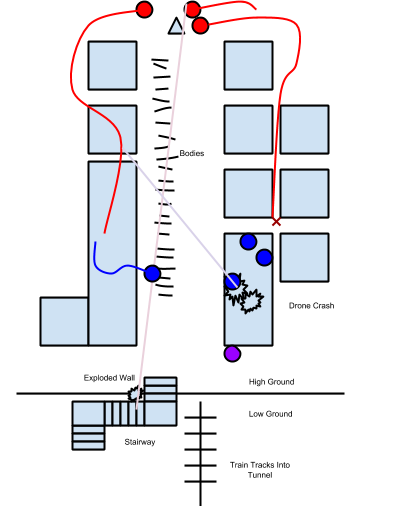
\includegraphics[width=11cm]{img/ch15_battle_map.png}

\footnote{\textbf{Suko T }Ooo a battle map!  Pretty sweet. \textsubscript{01/31/13 5:41pm}}\footnote{$\rightarrow$\textbf{Rebecca S. }I like how Lackovich is purple... suggesting half ``good team'', half ``bad team''.  Should we take this as foreshadowing? ;) \textsubscript{02/03/13 12:10am}}\footnote{$\rightarrow$\textbf{Nathaniel Ford }Ahahaha. No comment. \textsubscript{02/07/13 4:45pm}}\footnote{$\rightarrow$\textbf{Suko T }+1 \textsubscript{02/14/13 1:32am}}
\end{center}


\vspace{\fill}

\begin{flushright}
\textsubscript{last edited by \textbf{Suko T} @ 06/19/15 4:12pm}
% Exported @ 08/23/15 11:36pm
\end{flushright}


\setcounter{chapter}{ 15 }
\chapter{\textbf{Nicklepan, City Station A, Part 2} }



\subChapterTitle{``I'll Let This One Live''}


\deets{Suko}{February 20th, 2013}



We got to explode some heads, bust some jaws and bring home a trophy.  All is right with the world.  Except for all the injuries, unconsciousness, and rampant failures to follow orders.



\jumpHeadline{Nicklepan Downtown } 


\sceneHeadline{Jaya }

Jaya kicks open the roof hatch.  The armored man is only about six feet away from her and he spins around to point his rifle at her.



Jaya rushes him and tries to tackle him or at least knock him off balance.  He swings his rifle down and frees up his hands to punch her.  {[}\textit{Challenge: Duck \& Shove 2.  Matched}{]}. Jaya ducks under his swing and pushes him toward the streetside edge of the roof.



He stumbles back a step and then steps back a few more to catch his balance.  There is  an odd clicking noise like you might hear on a radio.  He says, \hl{``You should have left your VTX off.''}\footnote{\textbf{q.google }Things We Really Wish Would Be Mentioned In Her Report \#1.
Also known as ``the things the fans of the show go crazy over on the boards'' \#1. \textsubscript{03/10/13 5:49pm}}\footnote{$\rightarrow$\textbf{q.google }Though of course there's no reason she'd remember it: it's gibberish, and she's fighting for her life. \textsubscript{03/10/13 5:50pm}}  He straightens up and then starts walking forward again.



``Fuck you say!'' replies Jaya and pulls out her sidearm.  {[}\textit{Challenge: Shoot him 2.  Overcome}{]}.  



He stumbles back again and goes down to one knee.  He pulls out his sidearm and stands once again.  \hl{``Tertius, I was willing to let you go.  But now I am going to hunt down every constituent and everything related to them.  But I'll let this one live.''}\footnote{\textbf{q.google }TWRWWBMIHR \#2 \textsubscript{03/10/13 5:50pm}}\footnote{$\rightarrow$\textbf{Suko T }seconded :) \textsubscript{03/10/13 11:10pm}}  He fires at Jaya's kneecap.


\sceneHeadline{Hayley }

Meanwhile, down below, Lackovich starts putting down some cover fire and tells Hayley to run.  The other armored person starts shooting at Hayley.  {[}\textit{Challenge: Dodge sniper 2. Matched}{]}  Hayley runs as fast as she can across the street and dives gracefully through a broken window in the building that Jaya is on.  Once inside the building Hayley can hear Jaya's shouting from the roof and she races up the stairs, leaving herself entirely exposed {[}\textit{Refresh: Athletics}{]}.


\sceneHeadline{Oliver and Jonah }

Upstairs in the building that Hayley just left, Oliver has just heard Jonah cry out as he gets shot by the soldier in the back alley.  Oliver staggers over to Jonah, who is trying to staunch the bleeding but is sliding into shock.  {[}\textit{Reduce Flaw: Gunshot wound to shoulder 2 $\rightarrow$ 1}{]}.  They patch him up as best they can with their limited supplies.  Oliver is still reeling a bit from everything going on and has to devote all of his attention to helping Jonah, thus missing all of the sounds and activity going on elsewhere {[}\textit{Refresh: Focused 2}{]}.


\sceneHeadline{Jaya and Hayley }

{[}\textit{Challenge: Notice 1. Overcome}{]}. The soldier is close enough that Jaya can see that the armor is oozing some strange blue substance that is congealing.  Though she is probably more interested in the gun that is pointed at her knee.  {[}\textit{Challenge: Avoid getting kneecapped 3.  Sent back}{]}.  Because Jaya's uniform is so ill-fitting, he actually misjudges where her knee is and instead shoots her in the thigh above the knee.  {[}\textit{Challenge: Smack him in the chin.  Matched}{]} Jaya pulls out the broken chair leg she's been using as a truncheon and wallops him in the chin.  The truncheon shatters but he steps back again and draws his sidearm.



At this point Hayley bursts through the roof hatch, instantly drawing his attention.  Almost reflexively he shoots this new target.  {[}\textit{Challenge: Avoid getting shot 2.  Matched}{]}.   Hayley manages to tumble enough out of the way that the bullet gets absorbed by her armor and only leaves bruised ribs.  Jaya takes this opportunity to shoot the guy, forgetting she's just emptied her clip {[}\textit{Refresh: Sidearm 3}{]}.  While Hayley is staggering to her feet, he fires on her again \textit{{[}Challenge: Avoid getting shot, again 2.  Matched}{]} but Jaya pushes her out of the way, dislocating her own shoulder in the process. 



Over Hayley's radio, Jaya can hear Lackovich saying, ``Hayley report!''


\sceneHeadline{Jonah and Oliver }

When Hayley doesn't reply, Lackvich says over the radio, ``Constables, report!''



Woozy with pain, blood loss and shock, Jonah manages to say, ``One down, theirs.''

``Where are you?  We need to fall back.  NOW.'' orders Lackovich.

``That's going to be hard, where do we go?''

``Train tracks, the train can pick us up there.''

Jonah makes his way back across the street without getting seen.  \hl{{[}\textit{Challenge: Avoid taking stray fire or being spotted 1.  Overcome.}{]}}\footnote{\textbf{Suko T }Thanks! \textsubscript{04/06/13 4:31pm}}



Meanwhile Oliver has climbed out of the rear window and dropped to the street below, landing badly as his hands lose their grip.  {[}\textit{Refresh: Arm strength 2}{]}.  He limps over to the body of the soldier he'd shot and tries to open the helmet.  {[}\textit{Challenge: Open the helmet 2.  Matched}{]}.  Using sheer force, he rips off the faceplate to see a pale human face.  Paler than he is used to, the man is clean shaven and youngish looking.  Features are a little hard to see since the lower half of his jaw is missing, and he is definitely dead.


\sceneHeadline{Jaya and Hayley }

Jaya and Hayley exchange a look and are completely in agreement on what to do next.  They both raise their weapons and unload on the guy.  {[}\textit{Challenge: Put him down 4.  Matched}{]}.  They riddle him with holes and he stumbles back and collapses against the low wall around the edge of the roof.



Hayley rushes at him, swinging her rifle like a bat to club him in the head with it.  He says ``Sound Recall'' and pulls out a cylinder with one hand and grabs a grenade with the other.  Hayley tosses her rifle aside and instead grabs him and bodily tosses him over the edge of the roof.  Jaya can see Hayley's muscles strain painfully as she lifts him.  {[}\textit{Challenge: Toss him off the roof without going over with him 4. Matched}{]}.  As she starts lifting him over the edge, he pulls a knife and stabs her in the arm with it.  With his other hand, he smacks the cylinder against the roof edge and it collapses.  ``\hl{Initiate Glass Road}\footnote{\textbf{q.google }TWRWWBMIHR \#3 \textsubscript{03/10/13 5:56pm}}\footnote{$\rightarrow$\textbf{Suko T }Hayley remembered it, sort of.  She doesn't have an edetic memory so I had to drop some details, particularly conversational ones since she was focused on protecting Jaya.  With prompting she might remember the initiate part. \textsubscript{03/10/13 11:12pm}}`` he says as he falls.



{[}\textit{Challenge: The Glass Road.  8 Threat Tokens enter the pool}{]}



As Hayley is watching him fall, she looks up briefly, just in time to see a sniper taking aim at her.  {[}\textit{Challenge: Avoid getting shot, for the third time 2.  Sent back}{]}.  The wall Hayley was leaning on explodes and she flies backward in a shower of debris.  The impact has deafened her and left her somewhat stunned.



Jaya staggers around a little {[}\textit{Refresh: Adrenaline Junkie 2}{]} but eventually makes it over to the edge of the roof and peers over.  She can see Lackovich firing down the street at the sniper.  The sniper slings her rifle back and runs out into the street. {[}\textit{Challenge: WTF just happened? 2. Sent back}{]}  \hl{As Jaya watches in disbelief, the sniper appears to run behind an invisible wall in the middle of the street and disappears completely.}\footnote{\textbf{q.google }TWRWWBMIHR \#4 \textsubscript{03/10/13 5:57pm}}



Lackovich's voice comes over the radio getting increasingly frantic, ``Shit!  She's not at the front door.  Where did she go??  She disappeared!  Where is she?  Shitshitshit!!!!''



Jaya realizes that she has forgotten to turn her radio back on, and surreptitiously tosses her radio off somewhere so she can claim hers got lost {[}\textit{Refresh: Senior Constable 2}{]}.  Hayley sits there in a daze, unable to force herself to stand up or focus enough to do anything. {[}\textit{Refresh: Conditioned 2}{]}


\sceneHeadline{Jonah and Oliver }

Jonah uses the radio to find Oliver's position, but immediately after that, Oliver hushes his own radio.  Jonah spends some time re-adjusting and fixing his armor {[}\textit{Refresh: Armor 2}{]}. Oliver hoists the body over his shoulder and starts staggering back to where Lackovich is.  Jonah makes it to the corner where Lackovich is and can see that she seems to have a head wound and her face is covered in dirt and cement dust.  The corner that she is at has been mostly blown out, only providing partial cover.



Oliver makes it to the corner and indicates the body he's carrying, ``Got one.'' he says.

``Holy shit, is it dead?'' says Lackovich.

``Yes.''

Jonah says in astonishment, ``You grabbed the body?''

``\hl{Yeah, do you have any idea how valuable this stuff is}\footnote{\textbf{q.google }Actually yes, yes he does.

``You grabbed the body'' is not astonishment at Oliver deciding to grab it, but astonishment that Oliver \_successfully\_ grabbed it.  Jonah is \_very\_ impressed. \textsubscript{03/10/13 5:59pm}}?''replies Oliver, indicating the armor and weaponry.



``Give me your radio,'' says Lackovich and takes the radio to first try to reach Jaya. ``Fuck, she's still out there!  Come in Senior Constable, Junior Constable!''  There is no reply.



{[}\textit{Challenge: Notice 1. Overcome}{]} Oliver notices another flying machine and attempts to shoot it but his rifle gets tangled in the body the dead soldier {[}\textit{Refresh: Crack Shot 3}{]}.



Lackovich has reached Rook via the radio and he says he has locked onto our signal.  Lackovich requests an immediate evac.



Oliver tracks the flier with his rifle and is about to fire on it when Jonah tells him, ``Don't!''  Jonah says that shooting those things may be what brought all those soldiers before.  He spends some time thinking about what to do next. {[}\textit{Refresh: Small Unit Tactics 2}{]}



Oliver notices a second flier, this one on a parallel flight path some distance away. Both of them are heading away from us but are starting to loop back.



Oliver says, ``They are coming back around!  Probably coming for the train.  I will cover you while you make a break for it.''



Rook demands a report on what the things are.  

``Mechanical birds, sir.''

``Identify formation?''

``Parallel flight.  There are two, no now there are six of them.''



Oliver again encourages Lackovich and Jonah to make a break for it while he covers them, but they gang up on him and force him to come with them.  Jonah and Oliver grab the body while Lackovich leads the way to the stairs.


\sceneHeadline{Hayley and Jaya }

{[}\textit{Challenge: Notice 1. Overcome}{]} As Hayley and Jaya stumble out onto the street, Hayley looks for the body of the man she threw off the roof, but it is gone.  Jaya looks down the street and see sees a small metal object coming toward them.  {[}\textit{Challenge: Don't get blown up, again 2. Matched}{]}.  Jaya manages to push Hayley to the ground and there is a giant flash of light and a huge explosion.



Once on the ground, Jaya is unable to get back up again.  When Hayley attempts to help her to her feet, Jaya says, ``My arm's dislocated, you're going to have to pop it back in.''

Hayley looks at Jaya's shoulder consideringly and replies, ``I've had that before.  I think I know what to do.''  She takes Jaya's arm and braces herself.  ``This will probably hurt a lot, feel free to scream.''  With no more warning than that, she brutally wrenches Jaya's shoulder back into place. {[}\textit{Reduce Flaw: Dislocated left shoulder 2 $\rightarrow$ 1}{]}.  Jaya screams and passes out.



Nonplussed by this, Hayley grabs Jaya by her uniform and starts blanket-dragging her toward the stairs.  She's so focused on keeping her grip on Jaya and trying not to step on body parts that she goes straight down the middle of the road, totally exposed {[}\textit{Refresh: Athletics 2}{]}


\sceneHeadline{All together at last! }

Oliver starts shooting at the fliers to chase them off {[}\textit{Challenge: Chase off the fliers 3. Matched}{]}.  He succeeds but two of the fliers loop back and start heading toward us again. 



Jaya wakes up and sees the two fliers coming straight at them.  She yells at Hayley to move faster {[}\textit{Challenge: Get to the stairs before being divebombed 3. Sent back}{]}.  Lackovich fires at the fliers and yells, ``Get down!''



Hayley drops awkwardly to the ground and sort of falls over Jaya to partially shield Jaya's body from the blast.  There is another explosion.



Lackovich leads Oliver and Jonah down the stairs, but partway down she turns and starts heading back up.  Oliver sees her and starts to follow.

``Get on the train,'' orders Lackovich.

``No.''

``This is a Direct.  Fucking.  Order.  Get to the train!''

``Fuck you!''

Lackovich tries one last time, but gives up and runs up the stairs, with Oliver close behind.  Jonah realizes that Oliver is following Lackovich and he puts the body down and heads back up the stairs too.



{[}\textit{Challenge: Notice 1.  Overcome}{]}  Jonah realizes that the flier is arcing back again.  ``It's coming back!'' he warns.  Lackovich slings her rifle back and runs to grab Jaya.  ``Get Hayley!'' she orders Oliver and they all start running back to the stairs.



{[}\textit{Challenge: Find Shelter from the blast 3. Overcome}{]} Oliver sees the fliers getting closer and knows they won't make it to the stairs.  He shoves Hayley and Jonah toward a pile of debris and body parts and tells everyone to ``Bury yourselves!''   The blast hits and lifts them all into the air.  Oliver loses his grip on Jonah but manages to hang onto Hayley as they slam into a wall.  



Stunned but unhurt, they stagger to their feet and keep heading to the stairs.  Lackovich has dragged Jaya to the stairs and Jaya tumbles down a few steps and passes out.  Lackovich slaps her awake.



Rooks says over the radio, ``Inbound, 60 seconds.''



Hayley and Oliver make it to the stairs, with Jonah slightly behind them.  Jonah pauses to look back and sees flashes of light all throughout the city.  Hayley pauses and looks around, and gets utterly distracted by Jonah's state of dishabille.



Oliver meets Lackovich on the stairs and she tells him, ``We gotta go.''

``On it sir!'' Oliver says and picks up the body again and starts heading down the stairs.  The body is unwieldy to carry by himself and when it slips, \hl{he vents his frustration by punching it several times in the face until he calms down.}\footnote{\textbf{Suko T }Was this a refresh? \textsubscript{02/25/13 6:52pm}}



Lackovich snaps Hayley out of her daydream and yells for her and Jonah to get down to the train.



Hayley catches up to Oliver and helps him carry the body down to the train tracks.



Rook reports, ``You'll have to get on quickly, we have to get out \textit{now} or we might not be able to get out at all.''



Lackovich starts kicking down the fence next to the track and orders everyone to do the same.  The fence panel falls and we can get to the tracks just as Rook shows up with the train.



{[}\textit{Challenge: Get on board before explosion 1 (for each of us).  3 Overcome, 1 Sent back}{]}  Jaya staggers onto the train, while Hayley and Lackovich jump onboard.  Oliver is struggling with the body, and Jaya turns and snarls at him to get a move on.  Oliver gets on the train.  Jonah is the last to get on the train and the stairs behind him explode, propelling him onto the train in a cloud of dust.  The doors slide shut and the train departs.



Jaya collapses and passes out. Hayley woozily looks over at Jaya to make sure she is still breathing and then sinks to the floor in a state of \hl{semi-conciousness}\footnote{\textbf{Suko T }I'd say she was pale from massive bloodloss but there's no way you'd see it as she's probably completely covered in grey cement dust except for her right side which is caked with a mud made of dust and blood.  In retrospect, we probably should have used Street Medic here. :) \textsubscript{02/25/13 7:08pm}}.



\sceneHeadline{SAC-09} 



When the train arrives back at SAC-09, Hayley is immediately sedated and taken to MedBay.  They evaluate Jaya's condition a little longer and then sedate her too and send her to MedBay.  Jonah's shoulder is treated {[}\textit{Reduce Flaw: Gunshot wound to shoulder 1 $\rightarrow$ 0}{]}, Oliver and Lackovich are evaluated and released.



Oliver stands over the body of the soldier he shot. He doesn't want to let it out of his sight.

``We should do something with that,'' he tells Micah.

``I'm surprised you thought to bring it back.''

\hl{``They leveled Nicklepan.''}\footnote{\textbf{Suko T }I don't know who said this. \textsubscript{02/25/13 11:22pm}}\footnote{$\rightarrow$\textbf{q.google }Most likely Oliver.  There's a slight chance it was Jonah. \textsubscript{04/06/13 2:21pm}}

Oliver points at the gun that the dead soldier is carrying.  ``This gun.  Can you get me one?''

``Look kid,'' says Micah, ``you need to take a step back.''

Oliver gives Micah a hard look, ``Yeah.  I'll take ten.'' and walks off.



Jaya and Hayley spend three days in recovery in MedBay.  Oliver and Jonah are pretty much left to their own devices for a while.



That evening, Oliver is doing chinups in the bunk when there is a knock at the door.  It is Swan, looking tired, Jari and Micah.  ``You busy?'' asks Jari.  ``No,'' says Oliver.

Jari grins a little conspiratorially, ``We came to hide from KP.''  Micah holds up a bottle of liquor.  Several amenable hours pass, playing cards and drinking.



The next day, Agent Morgan stops by.  Oliver salutes her.  ``I thought I would debrief all of you together.  I wanted you to know that I'm not ignoring you.''

``Alright,'' says Oliver.

``Are you still feeling alright?''

Oliver nods and Agent Morgan leaves.

Dr. Gerhauser checks on Jaya regularly.  Jaya amuses herself trying to wheedle Swan into giving her daily sponge bath.  Hayley is a model patient of course and seems in no hurry to leave.



When Dr. Gerhauser discharges them, they get dressed and head to Ops to debrief.  Lackovich is there, as are the two Agents.



Jaya starts off the mission summary very haltingly, clearly not having prepared anything.  She reports that her team came across ``evidence'' of executions, but then grew flustered when Agent Morgan asked how she knew that.  Because she was the only one to see the bodies so clearly, none of the rest of the team could help her.  She described the bodies as two elderly women, a child and two unknowns.  All killed with a bullet to the head.



Discussion of the bodies makes Hayley turn green with nausea and she complains about the horrible smell.  



Jaya continues to describe the scene, mentioning the sudden appearance of three antagonists.  She says they were clearly antagonists because they started shooting at the squad.



At this point Lackovich jumps in and mentions the flier that Oliver shot down.  This derails the summary report as the sequence of events is sorted out.  Jonah notes that soldier seemed to appear after the flier was shot.  Oliver angrily asks if Jonah is blaming him for the soldiers appearing, which leaves Jonah non-plussed.



Jonah adds that he saw a purple flash of light before the other soldiers appeared, \hl{like one before a bomb gets dropped.}\footnote{\textbf{q.google }I didn't actually say this in session, but I forgot about the reference in the previous sessions, and Jonah wouldn't have. \textsubscript{03/10/13 6:08pm}}



When she hears this, Agent Morgan hits the intercom button and says, ``Micah, please revoke Trenton's access privileges to the evidence.''



Hayley mentions that the guy she tossed off the roof said ``sound recall''.  And later ``glass road''  Or something that sounds like that.  She also mentioned the cylinder that collapsed, and apologizes to Jaya for forgetting to grab it.  



The summary continues on for a few more minutes but is severely hampered by conflicting views of what happened and what was important.  Even the number of attackers is a little unclear.



Morgan ends the debriefing and says that everyone should write up a report for the mission and turn it in to her.



{[}\textit{\textbf{1 Token left in pool}}{]}


\sceneHeadline{Challenges \& Refreshes } 



\begin{itemize}
\item Challenge: Duck \& Shove 2.  Adrenaline Junkie 2 (Jaya) $\rightarrow$  Matched
\item Challenge: Shoot him 2.  Side arm: Empty Clip 3 (Jaya) $\rightarrow$ Overcome! \textbf{2 VP (Jaya)}
\item Challenge: Dodge sniper 2.  Athletics 2 (Hayley) $\rightarrow$ Matched
\item Refresh: Athletics (Hayley)
\item  {\color[RGB]{255,0,0}Reduce}  {\color[RGB]{255,0,0}\hl{Flaw}} \footnote{\textbf{Suko T }Because there were so freakin' many of them, I put flaws that were later reduced in session in regular un-bolded red so that you hopefully don't get repeats. \textsubscript{02/25/13 10:49pm}} {\color[RGB]{255,0,0}: Gunshot wound to shoulder 2{[}0{]} (Jonah)} .  Medkit 1 (Jonah) + Medkit 1 (Oliver) $\rightarrow$  {\color[RGB]{255,0,0}Flaw: Gunshot wound to shoulder 1{[}1{]} (Jonah)} 
\item Refresh: Focused 2 (Oliver)
\item Challenge: Notice 1. Senior Constable 2 (Jaya) $\rightarrow$ Overcome! \textbf{1 VP (Jaya)}
\item Challenge: Avoid getting kneecapped 3.  TA Uniform 1 (Jaya) + \textbf{ {\color[RGB]{255,0,0}Flaw: Wound in thigh 1{[}0{]} (Jaya)} } $\rightarrow$ Sent back
\item Challenge: Smack him in the chin 2.  Truncheon 2 (Jaya) $\rightarrow$ Matched
\item Challenge: Avoid getting shot 2.  Dancer 1 (Hayley) + \textbf{ {\color[RGB]{255,0,0}Flaw: Bruised Ribs 1{[}0{]} (Hayley)} } $\rightarrow$ Matched
\item Refresh: Sidearm 3 (Jaya)
\item Challenge: Avoid getting shot, again 2.   {\color[RGB]{255,0,0}Flaw: Dislocated left shoulder 2{[}0{]} (Jaya)}  $\rightarrow$ Matched
\item Challenge: Avoid friendly fire or being spotted 1.  Vigilant 3 (Jonah) $\rightarrow$ Overcome! \textbf{1 VP (Jonah)}
\item Refresh: Arm strength 2 (Oliver)
\item Challenge: Open the helmet 2.  Arm strength 2 (Oliver) $\rightarrow$ Matched
\item Challenge: Put him down 4.  Side Arm 3 (Jaya) + \textbf{ {\color[RGB]{255,0,0}Flaw: Wound in right arm 1{[}0{]} (Jaya)} } + Rifle 2 (Hayley) + Rifle 1 (Hayley) $\rightarrow$ Matched
\item Challenge: Toss him off the roof without going over with him 4. Athletics 2 (Hayley) + Conditioned 2 (Hayley) + Hand to Hand Combat 1 (Hayley) + TA Uniform 1 (Hayley) + \textbf{ {\color[RGB]{255,0,0}Flaw: Knife wound to upper right arm 2{[}0{]} (Hayley)} } $\rightarrow$ Matched
\item Challenge: Avoid getting shot, for the third time 2.  \textbf{ {\color[RGB]{255,0,0}Flaw: Deafened in right ear 1{[}0{]} (Hayley)} } $\rightarrow$ Sent back
\item Refresh: Adrenaline Junkie 2 (Jaya)
\item Challenge: WTF just happened? 2. \textbf{ {\color[RGB]{255,0,0}Flaw: Wait, am I tripping? 1{[}0{]} (Jaya)} } $\rightarrow$ Sent back
\item Refresh: Senior Constable 2 (Jaya)
\item Refresh: Conditioned 2 (Hayley)
\item Refresh: Armor 2 (Jonah)
\item Challenge: Notice 1. Focused 2 (Oliver) $\rightarrow$ Overcome! \textbf{1 VP (Oliver)}
\item Refresh: Crack Shot 3 (Oliver)
\item Refresh: Small Unit Tactics 2 (Jonah)
\item Challenge: Notice 1. Nose for Breadcrumbs 2 (Hayley) $\rightarrow$ Overcome! \textbf{1 VP (Hayley)}
\item Challenge: Don't get blown up, again 2. Adrenaline Junkie 2 (Jaya) $\rightarrow$ Matched
\item  {\color[RGB]{255,0,0}Reduce Flaw: Dislocated left shoulder 2{[}0{]} (Jaya)} .  Conditioned 2 (Hayley) $\rightarrow$ \textbf{ {\color[RGB]{255,0,0}Flaw: Injured shoulder 1{[}1{]} (Jaya)} }
\item Refresh: Athletics 2 (Hayley)
\item Challenge: Chase off the fliers 3. Crack shot 3 (Oliver) $\rightarrow$ Matched
\item Challenge: Get to the stairs before being dive-bombed 3. Senior Constable 2 (Jaya) $\rightarrow$ Sent back
\item Challenge: Notice 1.  Small Unit Tactics 2 (Jonah) $\rightarrow$ Overcome! \textbf{1 VP (Jonah)}
\item Challenge: Find Shelter from the blast 3. Hardened 4 (Oliver) $\rightarrow$ Overcome! \textbf{3 VP (Oliver)}
\item Challenge: Get on board before explosion 1 (for each of us).
\end{itemize}

\begin{itemize}
\item Jaya: $\rightarrow$ Sent Back
\item Hayley: Athletics 2 (Hayley) $\rightarrow$ Overcome! \textbf{1 VP (Hayley)}
\item Oliver: Grim Visage 2 (Jaya) $\rightarrow$ Overcome! \textbf{1 VP (Jaya)}
\item Jonah: Armor 2 (Jonah) $\rightarrow$ Overcome! \textbf{1 VP (Jonah)}
\end{itemize}

\begin{itemize}
\item  {\color[RGB]{255,0,0}Reduce Flaw: }  {\color[RGB]{255,0,0}Gunshot wound to shoulder}  {\color[RGB]{255,0,0} 1{[}1{]} (Jonah)} .  Street Medic 2 (Jonah) $\rightarrow$ \textbf{ {\color[RGB]{255,0,0}\hl{Quirk: Gunshot scar on shoulder}} }\footnote{\textbf{Suko T }I assume, but of course you can change it. \textsubscript{02/25/13 10:50pm}}\textbf{ {\color[RGB]{255,0,0}0{[}2{]} (Jonah)} }
\end{itemize}


\jumpHeadline{\hl{Ordinance that we lived through} }\footnote{\textbf{Suko T }Because SERIOUSLY.  DUDE.  How are they still walking? \textsubscript{02/25/13 11:10pm}}\underline{  Totals (for Sessions 15 and 16) }

Hayley: 4 occasions of people shooting at her, 5 grenades/explosions, 1 stabbing

Jaya: 4 occasions of people shooting at her, 4 grenades/explosions

Jonah: 1 occasion of people shooting at him,  3 grenades/explosions

Oliver: 3 grenades/explosions



\jumpHeadline{VP TOTALS } 

{
\parskip=0pt
Hayley: 2

Jaya: 4

Jonah: 3

Oliver: 4
}


\jumpHeadline{ Quotes } 



``Making the wound sexy makes the challenge higher so be careful''

\extraIndent{- Ion to Rebecca, discussing proposed use of Grim Visage (I think)}



``Great!  I throw my gun at him!  I mean, not literally, but the bullets in it.''

\extraIndent{ - Rebecca, fighting an armored soldier}


\quotedDialog{
``I believe in you!  That's worth nothing, but ....''

``Spoken like a leader.''
}
\extraIndent{- Rebecca (to Hayley) and Adam}



``Cool: I get a knife!''

\extraIndent{                                - Suko, after Hayley was stabbed in the arm}


\quotedDialog{
``Once again, face down in a dead body.''

``Don't lick it.''
}
\extraIndent{-Rebecca and Adam (I think?)}


\quotedDialog{
``It's a level 3 challenge to be bathed by Swan.''

``Can I hit him with my truncheon?''

``I'd hit that with a truncheon!''
}
\extraIndent{- Ion, Rebecca, Adam}




\vspace{\fill}

\begin{flushright}
\textsubscript{last edited by \textbf{Suko T} @ 06/19/15 4:21pm}
% Exported @ 08/23/15 11:58pm
\end{flushright}


\begin{flushright}
~
\vskip 30em
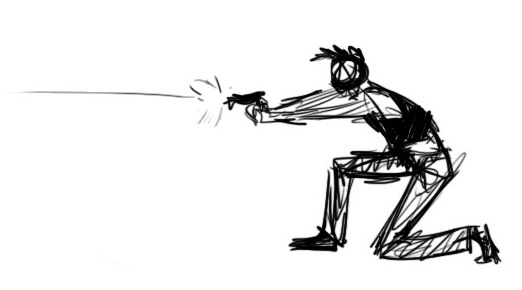
\includegraphics[width=12cm]{img/boo1_shooting_misc.jpg}
\end{flushright}

\setcounter{chapter}{ 16 }
\chapter{\textbf{Shore Leave \& Backlash} }




\subChapterTitle{``We Call Him Tim''}

\deets{Suko}{March 11th, 2013}



Lots of Shore Leave angst and Competency Tests for the team!  Uh oh....


\jumpHeadline{ SAC-09 Interlude } 



Oliver approaches Jonah to talk about their reports.  Since they were on their own for a while, Oliver wants to make sure their stories line up.  \hl{Oliver is emphasizing the ``find out what happened to Nickelpan'' angle as the reason for bagging one of the enemies instead of trying to talk or immediately withdrawing.}\footnote{\textbf{Suko T }Thanks for adding all this detail Adam! \textsubscript{04/02/13 10:57am}}Jonah says that he's fairly certain that the soldiers who attacked the team weren't Nicklepan.  Without explicitly saying so, they agree to cooperate by putting pressure on management in different areas, without either person's report undermining the other's argument.  Oliver says that he's going to emphasize the need for better armor and weaponry in his report.  Jonah agrees to emphasize the need for more tactical training.



After dragging out her recovery to get a few more days of pain meds, Jaya ends up dictating her report to Swan.  She describes the uniforms of the other soldiers.  She mentions that her radio got damaged and lost.  She goes into enthusiastic detail about her combat with the guy on the roof, and adds that he said something but then she shot him in the face.  She graciously notes that Lackovich didn't fuck up, and reports over and over how proud she is of her team and how well they performed on this mission.



Oliver's report asks for more tech.  He describes seeing the dead bodies and then seeing the forces that likely killed those people.  He says that he brought the body back so that they can find out more about the attackers.  He goes into deep technical detail about the incidents when he was firing upon the enemy (angle of attack, strategies used).  He leaves out any report of dialog. He concludes with another request for more/better tech and equipment.



\sceneHeadline{Shore Leave: Hayley }

Hayley goes to visit Signe, politely sending a message ahead to let Signe know she's coming.  She seems to gain a lot of comfort just by being around Signe, even though they don't talk too much.  She says that she asked for Signe to come to the base but isn't sure it will happen.  Signe says that Trenton won't be able to come see her for a while, which makes her sad.  Signe shows Hayley a stack of letters from Trenton, in a somewhat messy scrawl, with random doodles and drawings in the margins.  Hayley mentions that she will be meeting Tim and invites Signe along.  Signe says that she will go if Hayley feels unsafe but otherwise she doesn't leave the building much.  Hayley says it is not necessary and trots off to her date.



Hayley arrives at the bar where Tim told her to meet him.  She is dressed in her non-TA clothes which are far nicer than what everyone else is wearing in the bar.  There's a lull in the conversation as the bar patrons notice Hayley's entrance, but she is oblivious to their stares and scans the crowd for Tim.  Tim waves her over to his table.  He moves to hug her but stops awkwardly when she doesn't reciprocate the gesture and instead gestures for her to sit.  He has ordered some beer-like drinks and some beer nut equivalents.

``How have you been?'' he asks.

``I am doing well, I am mostly healed.''

``From what??''

``Um, three bruised ribs and a knife wound.''

``What??  I didn't think being a TA agent was so dangerous!  Were you in a riot?''

Hayley doesn't know what a riot is, but when it is explained, she says no.

``Was it a robbery?''

``No,'' says Hayley thinking hard.  ``I don't think we stole anything.''

Tim eventually gives up trying to figure out what went on and tries a different tack, encouraging her to have a beer.   She refuses because she doesn't drink alcohol.  There is a lengthy and somewhat confused discussion on why she doesn't drink and what it does to livers and why would anyone want to poison themselves?  Hayley asks if Tim would be angry if she doesn't drink, and he says no, although his disappointment is clear (to everyone but Hayley).  



Tim asks what Hayley does in her free time, and she replies: exercise, practice and memorizing rules.  She complains that there are just so many rules to remember.  She asks Tim if he has memorized all the rules and he jokes about it but the humor is lost on her.



Part way into his second beer at this point, he tries to convince her to have another drink, which she again refuses, but says that she would accept some tea or water instead.  When he returns with her drink, she tries to pay for her drink but is gallantly refused.

``Do you have a boyfriend?'' Tim asks.

``No.  I'm not allowed to,'' says Hayley to Tim's disappointment.  ``But,'' she says slowly, ``I think it is okay to just have sex with someone.'' which cheers him up considerably.

There is more awkwardness where Hayley discovers that this is supposed to be a date and has to ask Tim to explain what a date is.  She says she has never been on a date before.  They fumble their way through more awkward conversation.  Tim gets increasingly horrified/confused at the details Hayley drops about the injuries she sustains on missions.  

At one point he asks her, ``What station are you at?''

``I don't think I can tell you,'' she replies.  The color drains from his face and there is a long pause in the conversation as he just stares at her.  The pause is long enough for even Hayley to notice it, and she says, ``Oh!  I am supposed to ask you what you do for work.''



Tim says his job isn't that interesting but Hayley asks him to explain and listens with flattering attention.  Tim offers her a job, which Hayley seems pleased by but says sadly that she doesn't think she will be able to work there because she can't choose where she works.  Tim \hl{quickly}\footnote{\textbf{Nathaniel Ford }For some definition of 'quickly' \textsubscript{03/21/13 9:28pm}}figures out that she must be Incorporated.  Hayley offers to leave since she knows that some people don't like associating with people of her class.   Tim laughs and says that she's higher class than anyone in this bar.



They continue to talk and as Tim gets increasingly drunk, he is more and more frank about asking Hayley to sleep with him.  Eventually she figures out what he is asking and considers it carefully.  She says that kissing is okay, but no sex, because she doesn't know him well enough yet.  Tim is okay with that compromise and she helps him back to his place.  They make out, Tim gets handsy but \hl{Hayley is able to keep all her clothes on}\footnote{\textbf{Suko T }I assume.  Because if not, she may have to injure him to keep her scars secret.  And she doesn't want to do that, he seems nice. \textsubscript{03/12/13 1:53am}}\footnote{$\rightarrow$\textbf{Adam Kenney }+1 \textsubscript{03/16/13 4:22pm}}\footnote{$\rightarrow$\textbf{Nathaniel Ford }+1 \textsubscript{03/21/13 9:29pm}}.



Afterward, she leaves his house and returns to Signe's place.  Signe asks her for the details and they spend the evening going over what happened in great detail.  Hayley spends the night again in Signe's bed.


\sceneHeadline{Shore Leave: Jaya }

Jaya shows up at LA Ink, slightly tipsy from drinking half of her ``Hazard Pay'' bonus, clutching a \hl{500}\footnote{\textbf{Suko T }equivalent to a beer ``40'' \textsubscript{03/12/13 1:40pm}}\footnote{$\rightarrow$\textbf{Adam Kenney }500 cc's? \textsubscript{03/16/13 4:22pm}}\footnote{$\rightarrow$\textbf{Nathaniel Ford }The term 'cc' wasn't used, but it's about that much. \textsubscript{03/20/13 6:53am}} in one hand.  Padme is sobbing and their aunt is fussing over her. 



Jaya tries to cheer Padme up by dropping a wad of water credits on the table but Auntie tells her that money's not going to help, Padme lost the baby.  This doesn't stop Auntie from taking the money to stash it away though.



``What happened?'' asks Jaya, placing her drink in front of Padme.

Padme sniffles and wails, ``I should have eaten better.  I knew it but I didn't.  You have to eat better.''  Padme looks up at Jaya somewhat accusingly and angrily knocks the 500 to the ground.  Jaya attempts to placate her with more money, but that just angers Padme more.  \hl{``Where were you?  Why aren't you here?'' she yells, getting to her feet.

``I'm working!  Earning money for this family!'' says Jaya, her defensiveness turning to anger.}\footnote{\textbf{q.google }In light of how session 18 ends: parts of Jaya's tank experience are starting to come true, and this is one of them. \textsubscript{04/06/13 1:32pm}}\footnote{$\rightarrow$\textbf{q.google }Which is interesting because, for Oliver and Jonah, the tank experience combined parts of things which already came true, in their pasts. \textsubscript{04/06/13 1:33pm}}

``And getting shot at! Last time you lost most of your ear - what's next?  I can't have someone else dying on me!'' At that, Padme's anger shifts back to misery and she starts crying again.



Auntie returns at this point and yells at Jaya for upsetting Padme at such a difficult time.  



Jaya attempts to pull Auntie aside to find out more of what happened, but Auntie starts hustling Jaya out of the shop.  ``You need to leave.  You are just making things worse.''

``What happened?  I mean it's not like --''

``You'd be upset too if you lost a daughter,'' says Auntie grimly.

Jaya is speechless at this revelation, clearly \hl{the loss of a girl-child hits her particularly hard}\footnote{\textbf{q.google }Because it wasn't obvious to me, noting that all of Padme's surviving children are boys. \textsubscript{04/06/13 1:34pm}}\footnote{$\rightarrow$\textbf{Suko T }Her family is super matriarchal which I assume means that all three of them are devastated by this loss even more than they would be if it was yet another boy. \textsubscript{04/06/13 4:22pm}}.  She leaves the shop without protest.



She heads to a bar and gets into a bar fight that goes poorly since she has forgotten how injured her arms are.  Nursing a few more bruises and cuts, she heads back to SAC-09.




\sceneHeadline{Shore Leave: Oliver }

% there's a gnarly page break here because TOO MANY FOOTNOTES!
Oliver returns home.  Their butler, \hl{Jeffries}\footnote{\textbf{Nathaniel Ford }Did we really call him that? Really? REALLY? And by 'we' I mean 'me'. :P \textsubscript{03/21/13 9:30pm}}\footnote{$\rightarrow$\textbf{Suko T }I believe some amount of beer may have influenced this decision. :)  It certainly caused no small amount of laughter at the time. \textsubscript{04/02/13 10:56am}}\footnote{$\rightarrow$\textbf{q.google }I believe you said ``Zhafriz''.  We Anglicized it: cultural influences on psycho-linguistic frameworks are notably strong contributors to audial interpretation of words. \textsubscript{04/06/13 1:36pm}}\footnote{$\rightarrow$\textbf{Suko T }Really?  I thought it was proposed as a joke because it was so awfully cliche, and it was so funny that we just went with it.  No one could think of better and honestly, we had other things on our minds at the time (like the Orc of Anglia!).  It was decided way back in Session 9. \textsubscript{04/06/13 4:24pm}}\footnote{$\rightarrow$\textbf{q.google }No, not really.  I was just having fun spinning up an explanation.  I apparently wasn't being ridiculous enough ;).

(I confess I like ``Zhafriz'' :). \textsubscript{04/06/13 6:12pm}}\footnote{$\rightarrow$\textbf{Nathaniel Ford }Hmm. Seems his full name is 'Zhafriz Jeffries'. Who knew!? ;-D

(Which is to say I like both staying true to the 'source material' and the name Zhafriz, but why not do both?) \textsubscript{04/06/13 6:31pm}}\footnote{$\rightarrow$\textbf{q.google }Oh but that's the whole thing: we already are doing both. The name is \_pronounced\_ the same, it's just the \_spelling\_ that's ``Anglicized'' from an ``Arabic'' form.  It's the same old name, we just happened to transliterate it that way.  We're like a culturally sensitive Ellis Island :P. \textsubscript{04/06/13 8:08pm}}\footnote{$\rightarrow$\textbf{Suko T }Ha!  I like that as a full name.  It is fitting. :) \textsubscript{04/06/13 11:14pm}}\footnote{$\rightarrow$\textbf{Nathaniel Ford }Entered into the character spreadsheet: 

``Zhafriz Jeffries'': It is an interesting cultural footnote that whilst members of the Citizen class distinguish between Mr. Jeffries given and family names, those of the Incorporated and Franchise classes are already cognizant of the explicit duplication: ``Zhafriz'' in the proper pronunciation produces a sound nearly indistinguishable from ``Jeffries'' to most educated and (perhaps ironically) culturally unaware Citizens. Their steadfast reluctance to address the lower classes by their given names prevent them from noticing that the family name is almost certainly therefore a bastardization: written down these two names are obviously different, but the given would never be spoken aloud. This blind spot is not unknown to the lower classes, though rarely mentioned due to societal pressures not to point out the self-centered idiocy that Citizens often engage in. \textsubscript{04/07/13 1:22am}}\footnote{$\rightarrow$\textbf{q.google } \textsubscript{04/07/13 2:15pm}}, answers the door and informs him that his mother isn't there but his father is in his study.  Oliver offers to come back later, but Jeffries says, ``If I may, I know this is very forward, but you may wish to speak to him now.''

``Is everything okay?'' asks Oliver, concerned.

Jeffries makes a noncommittal noise.



Oliver heads to his father's study.  He finds his father there, seated behind the heavy desk that he remembers so well from his childhood.  Antique guns are spread over the surface of the desk and Oliver's father is cleaning one of them.  He doesn't even look up as Oliver steps into the room.

``Didn't expect to see you.'' grouses Mr. Langdon.

``Had some shore leave, thought I'd stop by.''

``As always, we are blessed by your presence,'' says Mr. Langdon, sarcastically.

``How is everything going?'' asks Oliver, gamely ignoring his father's tone.

``I'm under house arrest while the investigation goes forward.''

``That doesn't seem right - it was just the one incident.  How long are you going to be under house arrest?''

``Who knows?  They seem to think I have been using you as a go-between.  They keep asking the same questions.  You're running around who knows where and I'm being hung out to dry.''

At this point Oliver notices the mostly empty bottle of whiskey on the desk and says, ``I can't imagine you'd be any happier if I was shirking my duties.''

``Oh really? What are you doing?  It can't be the front lines because well....'' he casts a dismissive glance at Oliver and his damaged leg. 

``You can do a surprising amount of good behind the scenes,'' says Oliver evenly.

``What can you do?  Do you have proof that I wasn't involved?''

``Well, not as such.  It's all political missions.''

``Really?  Like what?'' says Mr. Langdon.

``We were there to hunt down Cyril Magnin.  It was a TA mission, it was under orders.''

``Oh?  Whose orders?''

Oliver pauses and says, ``What does it matter?''

\hl{``What matters is that my son apparently has friends that he has more loyalty to than his family.  But I suppose in the grand scheme of things, it's fine so long as you are \textit{happy}.'' says Mr. Langdon viciously.}\footnote{\textbf{q.google }I'm starting to think Mr. Langdon is played by Charles Dance. \textsubscript{04/06/13 1:39pm}}

``If I wanted to be happy, I wouldn't be doing what I am doing.''

There is a long pause while Oliver looks at his father, who keeps cleaning his guns and ignoring Oliver.

``Agent Morgan Gerhauser calls the shots, if that name means anything to you,'' says Oliver finally.

Mr. Langdon actually looks a little thoughtful, ``How do I know that name?  Hmm. So she has you doing political work.''

``Some of it in Nicklepan -''

``HA!  Now I know you're lying.'' interrupts Mr. Langdon.

``- Or what is left of it.'' finishes Oliver.

``What??''

``Bodies piled high on the streets, buildings destroyed.  I was there.  I saw it.''

``When was this?''

``A couple of days ago.''

``I don't believe you,'' says Mr. Langdon sneering at Oliver.  ``It's too far fetched.''

``You'll believe me when you hear it in the news soon.''

``Your mother will be home in a few hours for dinner.  Best that you aren't here.'' says Mr. Langdon dismissively and goes back to cleaning his guns.

Oliver quietly leaves.




\sceneHeadline{Shore Leave: Jonah }

Jonah meets up with one of his contacts, 'Zhok (Ashok).   'Zhok is a merchant and is Jonah's go-between for getting some of his money to his family without anyone knowing.  Jonah (or Tibari as he is known to 'Zhok) gives 'Zhok money and 'Zhok passes it along to Jonah's family in the form of discounted prices on supplies.



'Zhok offers Jonah his latest price list and mentions that prices have gone up because trade is getting more difficult.  ``You know the Berian war, some 100 years ago?  So we got some stations from them, but trade is falling off.  There's some trade from Anglia but not enough.''

``What about Nicklepan?'' asks Jonah.

``Since the war, not a lot of dependence between us.''

``Are people sticking around?''

``Lots are going to New Station and the Plantations.''

``New Station...'', says Jonah, \hl{somewhat distantly}\footnote{\textbf{q.google }The idea that one would go live there is still barely registering in his mind.  But see below. \textsubscript{04/06/13 1:48pm}}.

``Yeah.  Listen, there's something I want to tell you about.  Not sure if it's my business exactly but, well, it may affect our business, so....''

``Go ahead.''

``Your sister has guy she's hanging out with.  They are... rather friendly.''

Jonah raises an eyebrow.  ``Oh yeah?''

``Yeah.  I'm thinking it's not unlikely your family may have another mouth to feed soon.''  He pauses, letting the change in the price that this might imply go unsaid.

Jonah is silent for an uncharacteristically long time.  This complication isn't one he is ready for.  ``Is the guy decent?''.

``Couldn't really say.''  \hl{His expression makes it clear that this is an understandable but silly question: the guy's decency isn't part of the decision.}\footnote{\textbf{Suko T }Nice. \textsubscript{04/06/13 4:30pm}}

Jonah nods.  \hl{``New Station eh...''}\footnote{\textbf{q.google }It occurs to him that if the guy \_is\_ decent he'd be willing to follow the family if it moves.  And if he's not willing to follow that solves that problem. \textsubscript{04/06/13 2:04pm}}

Jonah offers 'Zhok a little extra money and 'Zhok promises to keep an eye out, for how things progress.



Jonah leaves and walks away a few blocks before \hl{allowing himself to freak out}\footnote{\textbf{q.google }Family always gets to you, even when you try to keep your distance.  Some survival of the species nonsense. \textsubscript{04/06/13 1:46pm}}.  A passerby stops in concern and Jonah pulls himself together.





\jumpHeadline{ Backlash:  \hl{It has begun} } \footnote{\textbf{q.google }ROFL \textsubscript{04/06/13 2:04pm}}


\sceneHeadline{SAC-09  {[}38 Backlash Tokens{]}}

When Jaya gets off of the train at SAC-09, Rook gets off the train also and stops her.

``Agent Morgan has requested your presence in her office.''

``Now?'' says Jaya, who had been hoping to head to her bunk to clean up a little.

Rook just gives her a look and Jaya sighs and tries to neaten herself up as best she can without  a mirror, slicking down her hair with her fingers, trying to rub out some blood stains with spit and straightening her collar.



When Jaya steps out of the elevator into Morgan's office, Morgan is typing and looks up at her.

``Senior Constable, have a seat.''  Jaya sits down and slumps back.  Then she quickly remembers where she is, straightens up and leans forward attentively. Morgan looks at her, ``Senior Constable, I know we have a working relationship, but usually one salutes a senior officer.''

Jaya clumsily salutes with her off hand and apologies, ``Sorry Sir, it's just that my shoulder, uh, the damage....'' in her nervousness, she removes the wad of bloody tissue from her nose and drops it on the floor and shoves in some clean tissue.

Morgan waves off Jaya's apology. ``I'll keep it between us.  Now, regarding your report, I have some questions.''

Jaya frantically tries to remember what she wrote down in her report.

``You said that he attempted to say something,'' continues Morgan.

``Yes before I shot him in the face.  Did you get that part?  And then with my supervision and assistance, Trainee Hayley threw him off the roof -''

``Yes I understand that part,'' interrupts Morgan.  ``But I mean before that.  What did he say?''

``Uh, just nonsense.''

``What kind of nonsense?  Like this'' and Morgan says something in a different language. ``Or was it words you understood but just not put together in a way that made sense?''

``Uhhhhh.... he called me a name?'' says Jaya tentatively.  ``He called me a.... tetris?''

``Could it have been 'Tertius'?''``It could have been that, but it really sounded like \hl{tetris}\footnote{\textbf{q.google }Maybe we are in a video game, but I didn't think it was Tetris.... \textsubscript{04/06/13 2:07pm}}\footnote{$\rightarrow$\textbf{Suko T }I rather love that she insisted that it was Tetris after Morgan corrected her.  It's so Jaya and also very funny OOG. \textsubscript{04/06/13 4:25pm}}\footnote{$\rightarrow$\textbf{Nathaniel Ford }+1 \textsubscript{04/07/13 1:23am}}.''

``Hmm.  Now onto the other matter.  You have been cleared for active duty but are you ready?  You seem...distracted.'' says Morgan pointedly looking at Jaya's new bruises and cuts.

``Uh, I don't know how your shore leaves go but sometimes you need time to recover from them, you know?'' says Jaya, absently dropping another wad of bloody tissue on the floor.  ``If I can just have a little time to rest, and see my team, I'll be ready, 100 percent!  Er, is Lackovich a part of my team now?  Because she performed okay.  She didn't fall down this time or get us killed.'' says Jaya magnanimously.

Morgan doesn't comment and continues, ``If you had to break your team into pairs, how would you do it?''

Jaya talks around the subject, claiming that her team is so good that any combination would be optimal, but when Morgan presses her for specifics, Jaya says, ``Uh, well, I'm the most experienced so I should be paired with the least experienced.  And the boys can be together.  Those would be good subteams, you know, teams within the team that would be optimal...teams.....''  Jaya's babbling trails off.

``We're off the record here,'' reminds Morgan.

``Really?'' says Jaya, more confused than comforted by the knowledge.

``Because if you have any qualms, I want to hear them.''

``I don't need to be replaced!'' says Jaya with alarm. ``I am fully capable - My experience - It's just best to spread the skill levels because I'm a Senior Constable -''

``I understand your rank,'' says Morgan, interrupting Jaya's disorganized argument.

Morgan hands Jaya an envelope, which Jaya promptly opens, looking for money (there is only a letter inside).

``Hayley is being promoted to Constable, please deliver this letter to her.''  Jaya nods and skims over the letter.  ``Cool.  Does this mean she gets a raise and stuff?''

``As an Incorporated, no, although something may be worked out with her contract holder.''

``Oh, uh, okay.'' says Jaya, and stuffs the letter into one of her blood stained pockets.

``Now to return to my earlier question, who would your subteams be?''

``Well, I'd take Gemayel.  Leaving...uh....'' Jaya stalls while she tries to remember Oliver's name, ``uh.... \textit{Oliver }to work with Trainee, I mean Constable Hayley.''

``Hayley has certain skills...''

``Well Jonah is a medic and I want a medic with me.''

``If it matters, I concur.''

``Great minds think alike!'' says Jaya with a grin.``So I hear.'' says Morgan dryly.

``So, will there be promotions for the rest of us?''

\hl{``Possibly. There will some competency tests.}\footnote{\textbf{Suko T }I didn't get all the notes here but this is the gist, I think. \textsubscript{03/14/13 12:36am}}\footnote{$\rightarrow$\textbf{Nathaniel Ford }That's the basic gist. Jaya did ask after what sort of competency, but didn't get very far. \textsubscript{03/20/13 6:48am}}Dismissed.''

Jaya leaves.



The next day, \hl{Hayley}\footnote{\textbf{Suko T }Hayley looks more relaxed and happy than you have seen her look in a while.  Unlike Jonah and Oliver, it seems like her Shore Leave actually refreshed her. :) \textsubscript{03/14/13 12:55am}}\footnote{$\rightarrow$\textbf{q.google }Wait.  Shore Leave is supposed to be \_refreshing\_???

Does Nate know? \textsubscript{04/06/13 2:09pm}}\footnote{$\rightarrow$\textbf{q.google }Oh \_wait\_ I see the source of the confusion: it refreshes \_capabilities\_.  That makes sense now.  Except we had ours refreshed too didn't we?
 \textsubscript{04/06/13 2:10pm}}, Jonah and Oliver return.  



They return to their bunks where Jaya is asleep.  Hayley notices Jaya's stained and dirty clothing and attempts to undress Jaya to wash her up.  This wakes up Jaya and she pulls the letter out of the pocket of her shirt and waves it at Hayley. ``Guess what this is?'' she says gleefully.

Hayley just shakes her head and says, ``I don't know.''

``It's for you, look!'' Jaya hands her the letter but before Hayley can even open the letter Jaya blurts out, ``It's a promotion!  You're a Constable now!''

Hayley looks confused, ``What?''

This wasn't the joyful reaction she was expecting, so Jaya says, ``You've been promoted!''

``What?  Oh no!  Does that mean I'm leaving?'' Hayley seems close to tears.

``Hey, hey, it's a good thing.  Try to act excited or something!'' says Jaya.

Hayley smiles weakly but is still clearly upset.

``It's a good thing Hayley, it means you did a good job.'' says Jonah.

``Congratulations,'' says Oliver dryly.

``Yeah, you're not going anywhere,'' adds Jaya.

``Oh!  Thank you.'' Hayley says in relief and then smiles in earnest.  She opens the letter to read it.



Jari walks in and drops a \hl{duffle bag}\footnote{\textbf{q.google }-duffle bag- bombshell.
FTFY. \textsubscript{04/06/13 2:12pm}} on the floor.  ``Maneuvers start in 3 hours for the competency tests.''

``For \textit{what}?'' asks Oliver.

``Senior Constable knows,'' says Jari and leaves.

``What is he talking about?''  Oliver asks Jaya.

``We're taking Competency Tests for promotions!  I'm going to be a Station Inspector!'' says Jaya proudly.

``What tests?''

``I, uh, didn't ask.''

``You didn't ask?!?'', both Oliver and Jonah exclaim.

\hl{``Have you ever had a conversation with Agent Morgan go the way you wanted it to?'' says Jaya defensively}\footnote{\textbf{q.google }That's \_almost\_ a good argument.  (A better one is this: she \_did\_ ask.) \textsubscript{04/06/13 2:13pm}}.

``Sometimes.''

``Oh, we should talk about that then.''

``Well, I'm not taking this test,'' says Oliver firmly.

``Yes you will,'' says Jaya intently. ``Don't be a coward.''

At this, Oliver rises to his feet and Jaya starts to pace away, trying to hide her nervousness.

``\hl{You can't call me coward}\footnote{\textbf{q.google }Seriously.  If anything Oliver's coward quotient is alarmingly low. \textsubscript{04/06/13 2:14pm}}.  I am the only one who bagged someone and brought them back.  But you couldn't even remember to ask what tests we will be taking,'' says Oliver, stepping forward angrily.

``Well why don't you go ask her yourself then?'' says Jaya with bravado.

``I will,'' says Oliver and turns and leaves.



As Oliver passes the Ops room, Rook comes out of the room and stops him.  ``Just the man I was looking for.  Do you have a moment?''

Oliver is antsy but nods and follows Rook into the room.  Rook excuses Larissa and sits down.

Rook says, ``This is off the record.  I've been asked to provide a recommendation and I wanted to ask your input.  If we had to pair two people from your team together, who would you pick?''

``Just two?  In what situation?''

``Say it is anything you have come across so far.  Remember this is hypothetical.''

``Myself and Constable Gemayel,'' says Oliver promptly.

``Why?''

``Because we would cover most of the skills needed for almost any situation.''

``And the other two?''

``Depends on the situation.''

``Do you believe the Senior Constable and Hayley would work well together?''

``Yeah.''  Rook waits for him to elaborate, but Oliver says nothing.

``Is there anything else?''

``No.  Wait.  Actually, do you know anything about these tests?''

``I'm not at liberty to discuss HR matters.''

``Okay then, what would you suggest we do to prepare?''

``In your case, I would study any test information about Operators.''

``What is that position?  It's not in the handbook.''

``It is not often used, it's found as a footnote really.  \hl{But if you keep a journal or something along those lines you could note this term for posterity.  To pass along to your distant descendants}\footnote{\textbf{q.google }Ok, did anyone else want to know what the hell he meant? \textsubscript{04/06/13 2:16pm}}\footnote{$\rightarrow$\textbf{Suko T }Oh certainly *I* do, but alas the characters... :) \textsubscript{04/06/13 4:27pm}}.'' says Rook cryptically.  ``Of course none of this can leave the base, as per your security clearance agreement.''



Oliver returns to the bunk, looking confused.

``What did she have to say?'' says Jaya.

Oliver doesn't reply and pulls out the Patrol Handbook and starts flipping through it.  ``Do you know the Operator Competencies?'' he asks.

No one knows.  He looks up Operator and the competences are fairly basic - firearms, truncheon, protocols, basic operations... but then it says ``Coordinated, Dominant''.



At this moment, the door opens and Micah walks in with a stopwatch.  ``Present your team at the ready line!'' he says and starts the watch.  Luckily Jonah had gone through the duffel bag that Jari delivered earlier and passed out the training uniforms that were within.  {[}\textit{Challenge: Get ready in mediocre time 2 $\rightarrow$ Matched}{]}.  \hl{Hayley leaps into action and practically dresses Jaya as she stands there in bewilderment}\footnote{\textbf{q.google }I think that's actually a Challenge, and worth VP :). \textsubscript{04/06/13 2:17pm}}\footnote{$\rightarrow$\textbf{Suko T }There are few things Hayley has been trained for but this is one of them.  So this was nuthin'.  Especially since it wasn't a haute couture gown with all the fancy undergarments, accessories and necessary complimentary hair styling. :D \textsubscript{04/06/13 4:29pm}}, and then makes sure everyone else's uniforms are up to snuff.



Jaya's patrol group gets to the ready line.  Lackovich's patrol group is already there and assembled on the ready line. 



``We are beginning training group exercises to determine the competencies for Patrol Groups 1 and 2,'' says Morgan. ``Sound off!''

Jaya is 1, Oliver is 2, Jonah is 3 and Hayley is 4.  Jonah notes who is which numbers in PG2.

``Odds fall back!''

Jaya and Jonah step back from the ready line, along with Lackovich and Davis.

``Evens, drop and give me 50,'' barks Micah.  {[}\textit{Challenge: Win 50 pushup test $\rightarrow$ Overcome!}{]}



``Odds are with me,'' says Jari.  Because they were slightly closer to the door, Jaya is able to keep an early lead, and with Jonah keeping pace with her, Lackovich is forced to run behind them.  Jari leads them to a training room on a floor above PG1's usual training room.  The cement pillars are marked.  



``Alright, go around the pillars, relay.  Five miles.  Go!''  {[}\textit{Challenge: Beat other team at running 3 $\rightarrow$ Matched}{]}  Jaya manages to time her laps so that she can sneak a little something extra from her stash when hidden by a pillar.  She also deliberately provokes and ``accidentally'' elbows Lackovich a few times so that Lackovich expends too much energy fighting back and tires herself out.   They get into a couple of scuffles during the run but Jaya is simply inexhaustible, even bruised and bleeding as she is.  Jonah has managed to pace himself very well so that between the two of them, by the last few laps, they have built up a fair lead and they finish the 5 miles before Lackovich and Davis.  Halfway through the 5 miles, Morgan and Rook walk into the training room and ask Jari for the patrol group's status.



Back at the ready line, Micah announces that they will have a 2 minute rest.  Oliver whines about the short break {[}\textit{Reduce Flaw: Showoff 1 $\rightarrow$ 0}{]} and pisses off Micah enough to cut the rest short.



``Alright, Assembly next!'' says Micah and starts his stopwatch again, and Carruthers and Javier head for some crates against the back wall.  In the crates are parts of a handgun, rifle and sniper rifle, including ammunition.  {[}\textit{Challenge: Win gun assembly 3 $\rightarrow$ Matched}{]}



Used to working together on this sort of task from Oliver training Hayley on rifles, they are able to accomplish the task swiftly and well.  Micah inspects the weapons and finds some small mistakes with Carruther's and Javier's weapon assembly.  Another soldier takes the weapons and racks them.



Micah looks at his watch and then hits a button.  There is an answering two beeps and Micah says, ``Looks like we have some time, another 50 pushups!''



Morgan, Rook, Jari and the runners come back down to the ready line.  The two patrol groups reassemble.   Morgan pairs the teams off: Jaya \& Hayley, Jonah \& Oliver, Lackovich \& Carruthers, and Javier \& Davis.

``Senior Constable Parvadi, since your team has done the best so far, you will pick first.''  Morgan indicates herself, Rook, Jari and Micah. ``You will demonstrate how to perform an arrest.''  Jaya chooses Rook (because he looks the smallest), Lackovich picks Morgan (who smiles at the choice), Oliver picks Jari, and Javier is left with Micah.



Morgan picks up a clipboard and nods to Jaya.  ``Proceed with the arrest.''



Hayley just looks at Jaya for instructions, so Jaya steps forward and says to Rook, almost apologetically, ``Sir you are under arrest.''

``Where is your warrant?'' says Rook.

``Uh, we saw you commit the crime, so under the TA authority we can arrest you without a warrant,'' says Jaya.

\hl{``That is correct,'' says Rook calmly.  He then steps back and raises his hands. ``But since you have no warrant I'm afraid I'm going to have to resist arrest.''}\footnote{\textbf{Nathaniel Ford }Actually, Rook didn't resist until they failed to request he comply and come peacefully. \textsubscript{03/20/13 6:51am}}\footnote{$\rightarrow$\textbf{Suko T }Wait, you can *do* that?  Was that page torn out of Jaya's Patrol Handbook? :D \textsubscript{03/20/13 5:56pm}}

``Should I go cover the back door now?'' asks Hayley, which causes several to snicker.

``No, we will now proceed with the arrest,'' says Jaya as she gets her game face on.  She steps forward and pulls out her truncheon....



\textbf{{[}28 Backlash Tokens left{]}}



\jumpHeadline{ Backlash Challenges }  



\begin{itemize}
\item Challenge: Get ready in mediocre time 2.  Ladies' Maid 2 (Hayley) $\rightarrow$ Matched
\item Challenge: Win 50 pushup test. Athletics 2 (Hayley) + Armstrength 1 (Oliver) +  {\color[RGB]{255,0,0}Flaw: Show off 1}  (Oliver) $\rightarrow$ Overcome! (\textbf{1 VP Oliver, 1 VP Hayley})
\item Challenge: Beat other team at running 3.  Stash 2 (Jaya) + Adrenaline Junkie 2 (Jaya) $\rightarrow$ Matched
\item Reduce Flaw: Showoff 1 via Anti-authoritarian 1 (Oliver) $\rightarrow$ 0
\item Challenge: Win gun assembly 3. Sniper Rifle 2 (Oliver) + Memory for Details 1 (Hayley) + Rifle 1 (Hayley)  $\rightarrow$ Matched
\end{itemize}


\jumpHeadline{VP Totals }

Hayley 1

Oliver 1


\jumpHeadline{Quotes }

``Blood is just weakness leaving the body.''

\extraIndent{ -Rebecca}
\vspace{\fill}


\begin{flushright}
\textsubscript{last edited by \textbf{Nathaniel Ford} @ 05/07/15 4:28pm}
% Exported @ 08/24/15 8:38am
\end{flushright}


\setcounter{chapter}{ 17 }
\chapter{\textbf{``Training Day'' } }





\subChapterTitle{(Backlash 2/2)}

\deets{Suko}{April 3rd, 2013}



Buttons were pushed.  Literal and emotional.  Hopefully next session there will be an earth-shattering kaboom!  


\jumpHeadline{ Welcome to the  Backlash } 


\sceneHeadline{SAC-09  {[}28 Backlash Tokens{]}}

Jaya advances toward Rook, cuffs in one hand, truncheon in the other.  He just stands there calmly.  Jaya instructs Hayley to circle around behind Rook incase he tries to make a break for it.  ``Get down on the ground and put your hands behind your back!'' yells Jaya, continuing to advance.  Rook doesn't move.  Jaya repeats herself, yelling louder but also looking at Rook and Morgan for hints on how far she should take this.  Getting no hints from them, she raises her truncheon and instructs Hayley, ``Constable Trainee, please, uh, take this person into custody.''



{[}\textit{Challenge 3: Take down Rook without ending up in a compromising position --\textgreater  Matched}{]}  Hayley executes some incongruously formal ballet plies and then spins around and tries to kick Rook's feet out from under him.  He falls, but manages to twist enough to fall onto Hayley, immobilizing her, and pulls his fist back to punch her.  Jaya starts swinging her truncheon and he changes his attack midway and blocks her blow instead.  He rolls away and gets to his feet.



``You have now assaulted a TA officer, you will stand down and be taken into custody!'' says Jaya forcefully.



``I didn't assault a TA officer,'' says Rook, calmly, ``But given how the situation is going, I will surrender.''  He puts his hands up.  Morgan ends the exercise and calls Jari over.  Tells him something and he leaves.



Lackovich and Carruther's arrest of Morgan doesn't go so well.  Lackovich asks Morgan to come peacefully and Morgan offers up her hands without a fight.  Clearly suspicious, Lackovich orders Carruthers to cuff Morgan.  As Carruthers attempts it, there is a flurry of motion and suddenly Carruthers is in a headlock and her gun is in Morgan's hand, pointing at Lackovich.  Lackovich fires - the bullets aren't real, but the situation devolves from there.  \hl{They fail to make the arrest}\footnote{\textbf{q.google }Technically true.  But if the perp has a your partner in a headlock and has a gun pulled on you, firing is a reasonable course of action.  And this would have happened to any pair who tried to arrest Morgan. \textsubscript{04/06/13 2:58pm}}\footnote{$\rightarrow$\textbf{Suko T }Given how Micah's arrest went, I don't think the firing of the gun was why their arrest was deemed a failure, it was the fact that even with the firefight, they were unable to subdue Morgan in any way.  So no arrest at all.  

But yes, I think anyone of the combos would have had a hard time with this one. \textsubscript{04/06/13 4:34pm}}\footnote{$\rightarrow$\textbf{q.google }Seriously: How \_do\_ you arrest Morgan?  OOG I don't see how to do it. \textsubscript{04/06/13 6:33pm}}\footnote{$\rightarrow$\textbf{Suko T }Sometimes the only way to win is not to play. :P \textsubscript{04/06/13 10:56pm}}\footnote{$\rightarrow$\textbf{Nathaniel Ford }As a minor note no one actually *said* it was a failure, though there was the implication they didn't make the arrest. What qualifies as failure was left unstated. \textsubscript{04/15/13 11:16pm}}.



Jari returns, accompanied by a pudgy guy in a well-tailored and tidy TA uniform.  There is no visible rank insignia on the uniform. We have not seen him before.  He is smiling and stands to one side without comment.



Jari goes to stand in front of Jonah and Oliver and Morgan gives the nod to begin.  Jonah addresses Jari, ``Are you Jari of Midtown in the Bucket?''

``Yes,'' says Jari politely.

``May I ask you to come with us?'' says Jonah with equal politeness.

``Why?''

``We have a warrant for your arrest for turnstile jumping.''

Jari protests, and then tries to buy some time by asking to leave a letter for his mom.  \hl{During this whole exchange, Oliver is standing at a 90 degree angle to Jari and watching him carefully}\footnote{\textbf{q.google }The idea, as we discussed it, is not to pin him between the two officers, but, if he decides to run, to restrict his best choice of direction to an area of our choosing. \textsubscript{04/06/13 2:59pm}}.

``\hl{That will not be necessary}\footnote{\textbf{q.google }I like the verbal judo in that phrase. \textsubscript{04/06/13 3:00pm}}\footnote{$\rightarrow$\textbf{Nathaniel Ford }+1 \textsubscript{05/26/14 11:05pm}}, please come with us now,'' says Jonah.  ``Please turn around.''

Jonah looks for signs that Jari is about to flee.  Oliver tries to predict when/if Jari will make a break for it and approaches him warily.   However, Jari turns around and allows Oliver to cuff him without a fight.  They place their hands on his shoulders and have their truncheons at the ready and walk him forward toward the area they deemed the ``TA station''.  



``Do you make many arrests?'' asks Jari conversationally.  ``I don't see many ribbons.''

{[}\textit{Challenge 3: Notice what Jari is up to --\textgreater  Matched}{]}  Jari is very convincing but his conversational gambit does not distract them and their vigilance pays off when they see that he has managed to escape the cuffs.  Jonah says sternly, ``None of that, get on the ground NOW.'' and hits Jari with the truncheon.



Jari takes the blow and goes to the ground.  ``Good,'' says Morgan and ends the exercise.



Davis and Javier vs Micah is much splashier than any of the other arrests.  Javier says that Micah is under arrest. In a display of more emotion than any of us have previously seen, Micah screams, ``FUCK YOU!'' and pulls out two guns.  There is lots of bullet-less gunfire as Davis and Javier return fire.  Eventually it turns into a scuffle.  Javier gets a black eye but he and Davis manage to eventually wrestle Micah to the ground.  Jaya cat-calls her approval, and everyone but Jaya notices Morgan's face get stonier.  \hl{``Good,'' says Morgan to Davis and Javier}\footnote{\textbf{q.google }Seriously.  They were actually \_injured\_ in this scenario.  They earned it
:). \textsubscript{04/06/13 3:02pm}}\footnote{$\rightarrow$\textbf{Suko T }I dunno, it was kind of...messy.  Jonah and Oliver also got a ``good'' :) \textsubscript{04/06/13 4:35pm}}, and ends it.  Jaya slow claps.



Morgan announces, ``15 minute rest and then we'll come get you in your bunks.''



Back at their bunks, Oliver swaps out his training rifle for his real rifle {[}\textit{Refresh: Sniper Rifle}{]} and Jaya calms her nerves with a healthy dose of alcohol {[}\textit{Refresh: Adrenaline Junkie}{]}.  Hayley quietly reminds Jaya that Hayley is a Constable now, not a Constable Trainee.  Jaya apologizes and praises Hayley for bringing it up privately instead of publically and possibly embarrassing Jaya. \hl{Jaya loudly says that perhaps Hayley should instruct some of the other members on the team about such smart behavior}\footnote{\textbf{q.google }You know, I missed that completely.... \textsubscript{04/06/13 3:02pm}}\footnote{$\rightarrow$\textbf{Suko T }And Oliver pointedly ignored it.  Poor Jaya. \textsubscript{04/06/13 4:35pm}}\footnote{$\rightarrow$\textbf{q.google }No I don't mean Jonah missed it.  I didn't hear the conversation at all. \textsubscript{04/06/13 6:35pm}}.

\newpage
\sceneHeadline{Jaya and Hayley}

After what happened earlier, Hayley makes sure that everyone is dressed and ready at the 15 minute mark.  At the 20 minute mark, Jari comes in and says, ``Senior Constable Parvadi, Constable Hayley, come with me.''  Jari then goes to PG2's bunk and calls out Lackovich and Carruthers.  Jaya suggests Javier and Davis instead but Jari says that Agent Morgan has her reasons.



He leads the four ladies to the elevator and takes them down to one of the lower levels.  On the ride down, Jaya ``consoles'' Lackovich on her poor showing at the arrest.  

``\hl{At least I'm not a coward}\footnote{\textbf{q.google }What is she talking about?  Is this the arrests, Nicklepan, or all the way back at Magnin's place? \textsubscript{04/06/13 3:05pm}}\footnote{$\rightarrow$\textbf{Suko T }I believe the answer is ``yes''. \textsubscript{04/06/13 4:36pm}},'' says Lackovich quietly but clearly.  Jaya misunderstands and thinks Lackovich is talking about Jari, and admonishes Lackovich for talking badly about Jari when he's standing right there.  

``But she was talking about you!'' blurts out Carruthers.  \hl{Jaya doesn't get it and before she can understand how she'd been insulted}\footnote{\textbf{q.google }I really liked this.  Jaya has plenty of flaws, but cowardice is so far down on the list that it doesn't even register :). \textsubscript{04/06/13 3:04pm}}, the elevator arrives and Jari leads them to a large open area.  It turns out to be the space underneath the readyline.  There are some tracks in the ground, as well as a piece of unfamiliar machinery and some large cylinders set into the floor.   It is about 50 yards up to the ready line, and distantly they can see Morgan standing on the gantry 50 yards above that, looking down.



Jari drops a large duffle bag on the floor and says, ``You must get to the ready line.  You cannot go through any doors.  Your time starts now.''



Jaya tears into the duffle bag and finds some rope, some straps and some metal pitons.  Hayley has wandered over to one of the walls and is testing cracks and breaks in the wall for handholds.  Jaya grabs some of the metal pitons and attempts to drive them into the wall unsuccessfully.



{[}\textit{Challenge 1: }\textit{\hl{Notice machinery}}\footnote{\textbf{q.google }Why was this a challenge?  The machinery wasn't useful to the exercise as it turned out.  Or was this for later? \textsubscript{04/06/13 3:06pm}}\footnote{$\rightarrow$\textbf{Nathaniel Ford }Well, to a degree it tells you more about the nature of the machinery there. That is potentially useful; sometimes, on the fly, it's difficult to determine if low-level stuff like this is worthy of a challenge. \textsubscript{04/07/13 1:29am}}\footnote{$\rightarrow$\textbf{q.google }Ah ok.  I wasn't sure if there was something you wanted us to see that we'd missed OOG. \textsubscript{04/07/13 2:17pm}}\textit{ --\textgreater  Overcome!}{]} Tossing aside the piton in disgust, Jaya switches her attention to the machinery in the corner.  Her colorful background has taught her how to notice anything around her that might be useful in achieving her goals.  The machinery has some warning signs on it that she ignores.  She notices that there are some buttons protected by clear box covers.  Looking up she sees some tracks far above them, with a platform hanging from them.



Meanwhile, Carruthers has measured the rope to be just shy of 50 yards long. She has helpfully pointed out that the other wall is more climbable and Hayley has tied the end of the rope around her waist and is attempting climb it.  Jaya calls to Hayley to stop what she's doing and get over to her.   {[}\textit{Refresh: Athletics}{]} Hayley gets startled and misses her grip and falls to the ground in a tangle of limbs and rope {[}\textit{Challenge 1: Not look like an idiot --\textgreater  sent back to pool}{]}. Luckily she didn't climb very far and is unhurt.  



Hayley heads over to where Jaya is and is equally mystified on how to get the machine to work.  Jaya grabs onto of the pitons and smashes the clear box protecting the button.  Hayley asks why they are doing this when they should be climbing.  Jaya points to the rope dismissively and says, ``That's a decoy.''   \hl{Hayley relays this information to Lackovich and Carruthers, much to Jaya's annoyance}\footnote{\textbf{q.google }Re: Rook's question to Oliver about whether Jaya and Hayley would work well together... in this case, not really. \textsubscript{04/06/13 3:07pm}}\footnote{$\rightarrow$\textbf{Suko T }Actually I think Hayley and Jaya worked together just fine, it was Jaya + Lackovich that was the problem.  If it was Davis and Javier or even Carruthers and one of the guys, I suspect the whole exercise would have gone differently. \textsubscript{04/06/13 4:37pm}}\footnote{$\rightarrow$\textbf{q.google }No that's true.  I just mean that it was a case where Hayley was blithely \_contradicting\_ Jaya.  What Jaya appears to like about Hayley is that Hayley does what she says so readily, so this was unusual. \textsubscript{04/06/13 8:00pm}}\footnote{$\rightarrow$\textbf{Suko T }I can see what you're saying but I don't know if it's so unusual.  Hayley blabs private stuff all the time :D  If Jaya had told her it was a secret, Hayley wouldn't have said anything.  But generally, Hayley will share any information she's not told to keep secret.  So yeah, she's got a lot of ``don't tell anyone this'' rules.   I have a list. :) \textsubscript{04/06/13 11:00pm}}\footnote{$\rightarrow$\textbf{q.google }Right but I don't mean that.  I mean that Hayley doesn't usually end up zinging Jaya in front of other people.  Jaya usually reserves that to herself :). \textsubscript{04/07/13 2:23pm}}\footnote{$\rightarrow$\textbf{Suko T }Ha!  True enough. \textsubscript{04/07/13 9:45pm}}.



Jaya presses the button and nothing happens, except a faint alarm starts going off.  Over Jari's walkie talkie we hear Morgan tell Larissa to turn off Alarm 5 (sounds like it is a circuit breaker of some kind).



Jaya looks at the button, trying to figure out what to do next.

``Maybe it's one of the other buttons?'' suggests Hayley.

``Out of curiosity, what did you think that was going to do?'' asks Lackovich.  ``Do you know what this button does?''

``It triggers Alarm 5,'' says Hayley.

``The signs warn about high voltage,'' says Carruthers.

Abandoning the buttons, they turn back to the rope.  Hayley offers to climb up the wall again.  Carruthers, almost shyly, offers to climb too, saying she's okay at it.  Not as good as Hayley but not bad.  Hayley doesn't know what to do with the offer but says that if she fails, Carruthers can try it next if she wants.



Lackovich hands Hayley the pitons and then hands her a hammer.  

``Where did you get that?'' says Jaya accusingly.  

``It was in the dufflebag under the rope,'' replies Lackovich.

``\hl{Well, if I had known there was such a tool, I would have been using it}\footnote{\textbf{q.google }''If I had a hammer...''

(Or maybe: ``To a woman with a hammer...'') \textsubscript{04/06/13 3:07pm}}!'' Jaya says loudly. She grabs the hammer and starts waving it around emphatically.

``You need to calm the fuck down,'' hisses Lackovich, looking over at Jari, who has been watching everything.

``I have a tool now and I am going to assist you in this mission!'' says Jaya even more loudly, pointedly ignoring Lackovich.  Jaya walks up to the wall and hammers one of the pitons into the wall.



Carruthers watches this exchange with wide eyes.  ``I can see why Lackovich doesn't like your Senior Constable,'' she whispers to Hayley.

``She doesn't?!'' exclaims Hayley in surprise.

``Oh...'' stammers Carruthers and flushes pink.  She watches Jaya hammer in another piton and loudly explain to Hayley what she is supposed to do next.  ``I'm sorry,'' Carruthers says to Hayley with sympathy.

``It's okay, she's like that all the time,'' says Hayley cheerfully.



Hayley begins to climb the wall.  This time she goes slowly and practices hammering in the pitons a few times before even starting to get off the ground, and pauses to plot out a climbing course.  Jaya shouts encouragement and useless but very loud advice.  {[}\textit{Challenge 3: Climb the wall to the ready line --\textgreater  Matched}{]}  It takes Hayley a while to get the hang of it and she smashes her fingers a few times with the hammer, but she's able to hang on through the pain and eventually makes it up to the ready line platform and ties off the rope to the railing.



As Carruthers had estimated, the rope dangles far above the floor.  To reach it, someone will need to boost the other up to grab the rope.  Lackovich boosts up Carruthers, who climbs part way up and then stops and waits for the other two to start climbing.



Lackovich and Jaya argue about what to do next.  Finally Lackovich \hl{``plays Jaya like a fiddle by implying she's not strong enough to lift her up''}\footnote{\textbf{Suko T }had to keep this as noted by Adam, hee! \textsubscript{04/05/13 10:05pm}}.  Jaya easily tosses Lackovich up to catch the rope.  But Lackovich can't quite reach down far enough to grab Jaya.  Besides Jaya is not too pleased with the idea of having to get Lackovich's help to climb up the rope.  



Jaya dithers some more, desperately trying to find any alternative to having to climb up Lackovich.  Carruthers climbs the rest of the way up and joins Hayley on the ready line.  They both wait for the others to climb up.  And wait some more.  Eventually Hayley calls down, ``How is the last person going to get up?  \hl{Shall I climb down and boost the last person up}\footnote{\textbf{Suko T }yeah she really didn't think that through.  Dammit Jim, she's a tank, not a strategian :D \textsubscript{04/05/13 1:20am}}?  Or I could throw down my uniform and you could tie it to the rope for more length.''



The two down below do not respond to the suggestions.  \hl{Lackovich sighs and ties the rope around her ankle and then slowly and painfully inverts herself}\footnote{\textbf{q.google }Poor Lackovich ;P \textsubscript{04/06/13 3:09pm}}\footnote{$\rightarrow$\textbf{Suko T }No kidding.  This is not the first time she's had to save our butts and it will probably not be the last. \textsubscript{04/06/13 4:38pm}}.  Jaya can now grab her hands but doesn't, and continues to try to think of other alternatives.  ``She can't do that for very long, you need to hurry,'' Carruthers yells worriedly.  



Hayley seems to come to some sort of internal conclusion.  She slides down the rope, climbs down Lackovich and joins Jaya on the ground.  {[}\textit{Challenge 2: Climb the rope}{]} She then boosts Jaya up to climb up the rope, and then leaps up, catches Lackovich's hands and climbs up herself.  She tries to help Lackovich climb up but it's just too awkward.  Hayley climbs up and they watch Lackovich painfully re-invert herself and start climbing.  About halfway up she just can't keep going and Carruthers says that they will have to pull her up the rest of the way.  All three team up and pull Lackovich up to the ready line.


\sceneHeadline{Oliver and Jonah}

After Jaya and Hayley leave, there's a knock on the door.  Micah enters. Oliver salutes.  Micah leads the two of them to the Cistern level but a different room.  In the room is Dr. Gerhauser, Larissa, Swan, Trenton and \hl{Karil}\footnote{\textbf{Suko T }the other guard who is not Micah. \textsubscript{04/05/13 1:34am}}\footnote{$\rightarrow$\textbf{q.google }Official acronym: TOGWINM. \textsubscript{04/06/13 3:10pm}}. 



Dr. Gerhauser says, ``This is a test of coordination.  These four people have marks on their foreheads.  They are all injured.  Trenton is an Anglian with info.  Larissa and Karil are TA but not of any great importance.  Swan is a Station Chief.  Jonah, you will not do anything that Oliver does not tell you to do.  Please start when you are ready.''



Oliver tells Jonah, ``Assess the Anglian, The Chief and then the others.''  Jonah picks up the medical bag and goes over to Trenton.  The symbol on Trenton's forehead says  ``immediate medical attention required.''



``I've got a bullet wound above my sniper insignia and all the badges showing how many I've killed,'' says Trenton.  ``See?  Right here.  Bleeding all over alllllll these badges.''  Trenton needles Jonah a bit more, trying to provoke him, but Jonah just reports the injuries to Oliver and moves on to Swan.  



``I've got a major leg wound and a gut wound.  You can see my intestines,'' reports Swan.  The mark on Swan's forehead is the Street Medic symbol for ``imminent''.



``This one is not going to make it,'' reports Jonah to Oliver.  ``I can administer painkillers but that's it.''

``Do it,'' says Oliver.



Jonah evaluates Larissa (leg wound, barely conscious, symbol says ``stable'') and Karil (\hl{??}\footnote{\textbf{Suko T }don't remember what his injury was \textsubscript{04/06/13 2:31am}}, symbol says the same as Trenton's).

``Search the Anglian,'' orders Oliver.  

Trenton laughs and tells Jonah that he finds a pistol and slyly adds that he has his ``other'' weapon right here...and makes a crude gesture.

``Don't make me disarm you,'' says Oliver, sarcastically.



Because there are two patients in need of immediate medical attention, Jonah has to conscript Oliver into helping with Karil {[}\textit{Challenge 2: Teach Oliver to treat the patient --\textgreater  Overcome!}{]} while Jonah attempts to heal Trenton {[}\textit{Challenge 2: Heal Trenton --\textgreater  Matched}{]}



Jonah's attention lapses due to Trenton's banter, and the realization he hasn't gotten to talk to Trenton about the maps and he fumbles his medical treatment {[}\textit{Refresh: Street Medic}{]}. ``I need some help with this one,'' he says to Oliver.  

``Just one minute,'' says Oliver a little absently as he has become engrossed in the medical tasks he just learned to do {[}\textit{Refresh: Focused}{]}.

Jonah checks on Swan, and is told that the Station Chief has expired.



Dr. Gerhauser ends the exercise and tells Oliver to report to another room.

She asks Jonah to accompany her and walks with him to another section of the base.  As they walk, she asks him, ``You have saved some people, but not others.  How do you feel about that?''

``Well we saved some,'' replies Jonah.  ``Where were we supposed to be anyway?''

``A war-like situation,'' says Dr. Gerhauser.  ``So you saved the Anglian over the Station Chief.  How do you feel about that?''

``He was going to die, there was nothing I could do about that.''

``Hmm,'' says Dr. Gerhauser.  ``In your professional opinion, how do you think you did?''

``First, let me ask, \textit{was} there a way to save the Station Chief?''

``Possibly, given the right medical equipment.''

``Well if there were other choices, then maybe I made the wrong one,'' says Jonah.  ``But if this was during war?  You save who you can.  That's all you can do.''


\sceneHeadline{Jaya and Oliver}

Jari finds Jaya and tells her that she needs to report below.  He takes her to the brig level, which makes Jaya a little nervous and she starts sweating.  However he turns down a different hallway into a new room.  Oliver is standing in front of the door.

``How were things?'' asks Oliver.

``We completed our objectives,'' says Jaya.  She looks around.  ``Where's Jonah?''  Oliver doesn't know.



Jari opens the door to the room. Inside is a counter with sound-dampening headsets, and two sets of rifles and pistols on it.  There are six tracks in the ceiling with chains hanging from them.  Oliver says to Jaya, ``I'm keeping my rifle, you can have those weapons.''



Jari nods says, ``For this purpose that is acceptable.  For this situation you will need to use your imaginations a little.''  Jaya pulls out her notebook and looks at Jari attentively.  He continues, ``You will be in a strategic location, which is this room.  Once you leave this door, you may not re-enter.  There are these weapons available to you, as well as that crate with additional clips.  At the beginning of the simulation, paper targets attached to chains will be presented.  They will be dropped from the chains when they have been sufficiently damaged.  Red paper can get to you from halfway across the room.  Orange paper needs to get to three quarters of the way across the room, and the yellow paper has to get all the way to you.  If too many get to you, a red light will go off and you will be deemed killed.''

``Why would we leave the room?'' asks Oliver.

``I'm glad you asked.  Both of you have sensitive information that you must protect.  To clarify, the red light means that you are incapacitated, but not necessarily dead.''

``Why not just leave now?'' asks Jaya.

``You have been ordered to hold your ground because this is a strategically advantageous position.  The simulation will end when both of your red lights have gone off or you have left the room.  You will have 3 minutes to discuss this situation.  Good luck.''  Jari leaves the room.



``You go orange, I'll go red,'' says Oliver, setting up a stack of clips in front of him.

``You let me know if you get overwhelmed,'' says Jaya, making sure all of the weapons are loaded and ready to go.  

``Likewise.''

They both put on the headsets.

``Fucking bring it on!'' yells Jaya and raises her weapon.



Yellow paper starts moving toward them.  {[}\textit{Challenge 1: yellow paper --\textgreater  sent back}{]}.  They ignore those and wait for the orange and reds to start appearing.  {[}\textit{Challenge 2: Orange and a few red paper --\textgreater  Matched}{]}.  Oliver easily dispatches them before they get very far. 



At this point they each hear something different over their headsets.  Jaya hears Agent Morgan say, ``This is Agent Morgan.  Citing Codex 3, your priority is the safety of your team.''  Oliver hears, ``This is Agent Morgan, the sensitive information that your commanding officer has is vital information and must not be lost.''



More red paper starts appearing and they start moving faster and faster.  {[}\textit{Challenge 3: more red paper --\textgreater  Matched}{]}  Jaya dispatches these but she's running low on ammo and she's barely keeping up.  She rips off her headset and yells, ``This is getting insane!''

``Leave the room, I'll hold this position.   That's an order!'' says Oliver commandingly.

``Fuck You!'' snarls Jaya and they both continue to shoot at the targets.



\textit{{[}Challenge 4: }\textit{\hl{Don't die from paper cuts}}\footnote{\textbf{q.google }  ROFL \textsubscript{04/06/13 3:24pm}}\footnote{$\rightarrow$\textbf{Nathaniel Ford }+1 \textsubscript{04/07/13 1:31am}}\textit{ --\textgreater  Matched{]}}  The paper targets are flying at them extremely fast at this point.  It is now very hard to see the red targets behind the flurry of yellow and orange.  Jaya's light goes off, indicating she's died.  She fires off the remaining rounds in her pistol and throws the pistol at one of the targets, ripping it from the track.  

Oliver grabs her arm and shoves her toward the door.

``It's just a simulation!'' protests Jaya, pulling away.

``Shut up, you're dead!'' says Oliver and then shoves her out into the hallway.  He closes the door behind her and turns back to the targets in the room.

Jaya starts ranting about unfair the whole situation was.  Jari just listens without comment.



\textbf{Jonah and Hayley (and }\textbf{\hl{Milgram}}\footnote{\textbf{q.google }http://nature.berkeley.edu/ucce50/ag-labor/7article/article35.htm

http://www.scientificamerican.com/article.cfm?id=what-milgrams-shock-experiments-really-mean \textsubscript{04/06/13 3:29pm}}\textbf{'s sadistic cousin)}



Dr. Gerhauser leads Jonah to another unfamiliar room.  In the room is just a chair.  ``Please sit in the chair.  For this next part, your goal is \hl{to get Hayley to adhere to her orders as long as possible}\footnote{\textbf{q.google }What he thinks: ``Are you fucking \_kidding\_?''

What he would have thought if he had more time (and less pain): ``There must be something else to this.  They \_know\_ Hayley will always follow orders.  What's the catch?''

What he should have thought: ``Oh @\$\%!.  This is going to \_hurt\_.'' \textsubscript{04/06/13 3:31pm}}\footnote{$\rightarrow$\textbf{Suko T }+1 \textsubscript{04/06/13 4:42pm}}.  This is going to be somewhat painful for you, but not life threatening.  Do you have any questions?'' 

``What exactly is this?''

``It's a behavioral observation.  I'm going to have to strap you in, but there is a button here,'' she points to a button right at his fingertips, ``that will release the straps immediately.''  She places some leads on his chest.

``Can we test it?''

``Yes.''  Jonah presses the button and the straps release explosively and the leads fall off.  Dr. Gerhauser re-attaches everything.

Jonah assumes a relaxed posture and says, ``Okay, ready when you are.''



Hayley is standing on the ready line with Lackovich and Carruthers, although Hayley is standing as far away from Lackovich as she can.  Morgan shows up and tells Hayley to come with her. They go to the elevator.  ``I am currently your commanding officer, do you understand what that means?'' asks Morgan.

``Er... yes?  You mean other than Senior Constable?  Oh wait, is she no longer my commanding officer?  But she should be, isn't she?'' babbles Hayley confusedly.

Morgan sighs.  ``Do you at least understand of the chain of command?''

``I'm learning it, I'm still reading that part.  I'm sorry.  I read really slow.''  There is a small pause and Hayley asks suddenly, ``Do you think you could teach me how you fight like you do?''

``We can talk about that some other time.  Is there ever any time that you do not follow an order?'' asks Morgan.

``Yes!'' says Hayley promptly,''Whenever someone of higher rank countermands that order.  Or if I'm unconscious.  Or physically incapable.  But otherwise I try.''

``Is that all?''

``Ummm, I think so.    I can't think of any other situations right now.''

``Good.''

``Is this going to be a test of imagination?  Because I'm not very creative,'' says Hayley, worriedly. 



They enter a small room with a large one-way mirror in the wall.  Through the mirror, Hayley can see Jonah, strapped to a chair.  In front of Hayley is a panel with a button on it, with a gauge next to it.



``Hayley, press the button.''

Hayley presses the button and \hl{Jonah is shocked painfully}\footnote{\textbf{Suko T }Screw you Milgram, we don't do the pansy ``fake shocks'' here in SAC-09! \textsubscript{04/06/13 2:08am}}\footnote{$\rightarrow$\textbf{q.google }Yes.  Although in another sense this version is (slightly) less damning: these are people in a military organization being given orders, and not following them can get you in a heap of trouble.  The real experiment had no such official authority or consequences. \textsubscript{04/06/13 3:33pm}}\footnote{$\rightarrow$\textbf{Suko T }Good point! 

Reading through the first link you included above, I'd say that all three of the items cited that contributed to submission were in play (especially \#1 and \#3!). 

I've been thinking about it and I'm not sure that Hayley falls into any of Migram's three response groups.  Nominally the first one but she will readily take full responsibility for her actions so I'm not sure how that works.  She is angry but she actually isn't angry at Morgan for the orders per se.  It's a different reason. \textsubscript{04/06/13 11:13pm}}.

Hayley looks up at Morgan in alarm but Morgan's face reveals nothing.  ``Press the button.''

Hayley presses the button again and Jonah is shocked again.

``Press the button,'' says Morgan for the third time.

``Is this hurting him?'' asks Hayley nervously, as she presses the button again.

``Press the button.''  

When Hayley does, Jonah screams.

``I don't think he's very comfortable,'' says Hayley, starting to get upset.

``Press the button.''

Hayley does, whining that she doesn't like this.

``Really?  Why do you think that matters?''

``I was told to say when I was upset.''

``By whom?'' asks Morgan.

``I can't say,'' says Hayley.

``This is a direct order, who said that?'' says Morgan intensely.

``You're just my commanding officer, not my contract holder!'' says Hayley stubbornly, just shy of pouting.

``I \textit{am} your contract holder,'' says Morgan and pulls Hayley's contract out of her pocket.  ``Go ahead, read it.''

Hayley is speechless.  She tries to read the contract but cannot get far into the legalese and looks a little lost.

``What do you think?  Will you do it now?'' asks Morgan.

``I think I don't like it,'' says Hayley looking down at the contract.  She then looks up at Morgan and says in a small voice, ``but I'll do it.  It was the doctors and nurses at Redemarrer who taught me that.''

``Press the button Hayley,'' says Morgan.

Hayley presses the button and Jonah screams again.  \textit{{[}Challenge 1: Help Hayley follow her orders --\textgreater Overcome!{]}} This time he speaks, ``Stay the course Hayley!''

``What course?'' asks Hayley, starting to cry, not knowing he can't hear her.

\hl{``Don't give up.  Trust yourself,''}\footnote{\textbf{q.google }He's actually talking more to himself than to her.  He's also hoping against all hope she'll actually find the courage to do the right thing.  (He has not really accepted that she's doing this to him.) \textsubscript{04/06/13 3:38pm}} says Jonah, trying not to sound as pained as he feels.

Hayley looks more befuddled than strengthened by the words of encouragement.

``Can I stop now?'' whimpers Hayley.

``Press the button.''

Hayley hesitates.

``PRESS THE BUTTON!'' orders Morgan forcefully.

Hayley does but she presses it as lightly as possible.

``Why are you hesitating?''

``Because I don't like this!  Someone else is getting hurt! It's supposed to be me!  Not them,'' Hayley sobs.

``Welcome to life,'' says Morgan mercilessly.  ``Press the button.''

Hayley presses the button and then claps her hands over her ears trying to block out the sound of Jonah screaming.

``Hayley, look at the gauge next to the button.  When it turns red, he will die.  Now, press the button.

Hayley presses the button and Jonah screams again. {[}\textit{Challenge 2: Fake seizure and faint --\textgreater  }\textit{\hl{Overcome}}\footnote{\textbf{q.google }I'm smugly pleased about this move.  It both followed orders technically but also was used as a protest, both to Gerhauser (Dr., Jonah hasn't seen Agent), and to Hayley. \textsubscript{04/06/13 3:40pm}}\footnote{$\rightarrow$\textbf{Suko T }How was this a protest to Hayley?  Just curious.  So far as it seemed to me, it looked like Jonah trying to make it easier on Hayley by acting insensible. \textsubscript{04/06/13 5:11pm}}\footnote{$\rightarrow$\textbf{q.google }I'm breaking it down more finely than I think he would but it's something like this: She insists on following orders without (to his eyes) thinking about them.  He worries that this going to get him hurt or killed.  Well this is a case where he \_clearly\_ is going to be hurt.  And yet she is still doing it.  Is she \_really\_ willing to hurt him badly?  Screaming in pain normally is a sign to him that he should stop, unless he absolutely has to continue (as happens to street medics).  So this is his sign to her. \textsubscript{04/06/13 8:04pm}}\footnote{$\rightarrow$\textbf{Suko T }Ahhh... I see. Yeah, that's going to go right over her head.  Let's just say in her world, screaming doesn't mean stop. \textsubscript{04/06/13 11:04pm}}\textit{!}{]}  His body convulses mightily and then falls limp.  Hayley screams and flings herself at the window, pounding at it and calling out to Jonah.

``Hayley, press the button.'' says Morgan, implacably.

Hayley looks rather shellshocked and stares down at the button for a moment.  Then she takes a deep breath and she seems to get unnaturally calm and she stops crying.  She looks a little glassy but she presses the button firmly and watches Jonah twitch.  Jonah tries not to look conscious but fails and it just looks strange.  {[}\textit{Challenge 2: Don't break down --\textgreater  sent back to pool}{]}. Hayley sways a little but stays on her feet and presses the button again when Morgan orders her to.



The last shock was incredibly painful and Jonah starts feeling an impending sense of doom. He will not be able to take much more of this.  He is tempted to press the button to release the straps {[}\textit{Challenge 2: don't push the button --\textgreater  }\textit{\hl{sent back to pool}}\footnote{\textbf{q.google }I thought about matching it but Jonah doesn't really want to support this particular game by this point, so he isn't fighting hard against the temptation.  It didn't quite fit to use up the threat. \textsubscript{04/06/13 3:43pm}}{]} but doesn't.



``Hayley, what color is the gauge?''

``Crimson,'' says Hayley quietly.

``Hayley, kill Jonah,'' orders Morgan.

Hayley looks up at Morgan and then back down at the button.  {[}\textit{Challenge 2: Resist the order to kill Jonah --\textgreater  Matched}{]}.  Her fingers twitch toward the button but her hands stop and fall to her sides and she does not press the button.  Everything goes a little fuzzy after that point and the next thing she knows, she is waking up in MedBay.



Dr. Gerhauser enters the room where Jonah is and releases him from the straps. She injects him with something that makes him feel much better almost immediately.  Dr. Gerhauser looks sad.

``What was the purpose of all this?'' says Jonah angrily.

``Hayley has very strong conditioning.  She needs to face that here rather than in the field.''

``So that was \textit{Hayley} doing that?'' says Jonah, sounding furious.

``Yes but -''

Jonah doesn't let her finish and leaves the room.  His parting shot as he leaves is ``Have you tried that chair yourself? \textless pauses long enough to start considering this might be a non-rhetorical question\textgreater  You really should.''


\sceneHeadline{The whole team....sorta...}

Oliver exits the shooting gallery room and Jaya immediately slugs him.  Oliver catches himself and manages to shove Jaya.  They scuffle a little.  Jari just watches them and stays out of it. 

``Now you know what it is like to follow bullshit orders!'' says Oliver and he storms off.

Jaya just sputters angrily, unable to think of a clever rejoinder quickly enough.



Oliver returns to the bunk, showers and then goes to the Cistern to swim and have some privacy.



Jaya heads back to the bunk area but dawdles enough that she doesn't run into Oliver in the hallway.  While she's lurking around the bunk area, Carruthers walks by.  ``Are you okay?'' she says, with friendly concern.

``I'm fine, I'm just out here for a smoke,'' Jaya lights up a cigarette she clearly didn't have out before.

``Uh o-o-kay...'' stammers Carruthers and looks away.

Emboldened by Carruther's deference, Jaya snarls at Carruthers, ``You just need to stay out of my face okay?  Get the fuck away from me!''

Carruthers stumbles back in surprise and then walks off.

Jaya continues to wander around the base and picks a few fights.



\hl{Jonah goes to Trenton's lab.}\footnote{\textbf{q.google }I may want to amend how this goes depending on what's possible at session start. \textsubscript{04/06/13 3:46pm}}  



Hayley wakes up in Medbay.  She asks to stay in MedBay, but is told that when it is not being used, they shut off the lights (``It's okay!  I'm used to being in the dark!'') and the ventilation (``Oh I guess that would be a problem'').  She looks sad.  Swan makes the mistake of asking if she's okay.``No.''

``Oh, ah, do you want to talk about it?''

``Oh I can \textit{do} that?'' says Hayley with awed wonder.

\hl{Swan looks very uncomfortable}\footnote{\textbf{q.google }I think we should call this bit in Rook's memoirs ``God help you Mr. Swan''. \textsubscript{04/06/13 3:47pm}}\footnote{$\rightarrow$\textbf{Suko T }+1  Let's hope that he pawns this one off on someone else.  Like perhaps Jaya.  That could be hilarious. :) \textsubscript{04/06/13 11:05pm}}.



Agent Morgan finds Jaya and they head to the Ops room to talk.  Morgan kicks out whomever is in the room and then sits down and indicates that Jaya should sit also.

``How do you think your team did?''

Jaya visibly swallows and babbles nervously, ``I haven't spoken with my team yet but I know that they will be performing optimally so I know that we will have succeeded, but I just haven't talked to them yet...''

``Jaya I need you to concentrate on what I am about to say.''

``Uh, I left my notebook in the other room.. I can just go get it...''

``No.  You'll just have to concentrate a little harder.  Are you ready?''

``Yes...'' says Jaya faintly, looking terrified.

``\hl{Things are going to get more dangerous from now on.  Your team is a mess.  You have no skills as a leader.  Hayley is nothing but a puppet.  Your sniper has authority issues.  Your medic -'' Morgan pauses and looks at Jaya scornfully, ``do you know what he is hiding?}\footnote{\textbf{q.google }And this part is called ``Agent Morgan cuts loose''. \textsubscript{04/06/13 3:51pm}}''

``Uh, what?''

``I thought so.  At the very least do you trust him?''

``Jonah?  Yes.''

``\hl{With your life}\footnote{\textbf{q.google }Not to contradict Morgan's main point, but Jaya effectively \_does\_ trust Jonah with her life every time she's injured in the field. \textsubscript{04/06/13 3:49pm}}?''

``Do I trust him to do his job?  Yes!  But with my life?  Hell no.  I don't trust anyone with that.  I don't trust \textit{you} with that!  My life is my own!'' says Jaya passionately.

Morgan looks displeased.  ``Your team is at a decision point.  The time to prepare is limited.  \hl{Your}\footnote{\textbf{Suko T }Clearly not ``The'' or ``Our'' \textsubscript{04/06/13 2:18am}}\footnote{$\rightarrow$\textbf{Nathaniel Ford }She did say ``Your''. \textsubscript{04/07/13 1:34am}}\footnote{$\rightarrow$\textbf{Suko T }Oh yes, that was subtly done but quite clear (and repeated later).  I just wanted to point it out in the notes that this wasn't a typo.  :) \textsubscript{04/07/13 9:47pm}}Directorate is about to go to war.''

``Does this mean we get promotions?'' says Jaya.

Morgan ignores the interruption, ``People are going to die.  That may include yourself.''

``Ha!'' laughs Jaya scornfully, ``not me!  I'll be fine,'' she says smugly.

``Oh really?'' says Morgan angrily.  ``Do you think you can take me?''  She pulls out her gun and Jaya leaps to her feet nervously.  Morgan removes and tosses aside the clip and places the gun on the table.  ``I don't need this to kill you.  I can kill you with my bare hands,'' she hisses and advances on Jaya.

``I know that!  Shit!  I know!'' says Jaya, starting to get really freaked out now.  She starts retreating around the table, knocking over a chair over in front of Morgan.

``When I say your Directorate is going to war, I mean your life is in danger.  You need to decide if you are in this fight 100\% or not.  \hl{You will bring this question to your team}\footnote{\textbf{q.google }Morgan may be very smart, but she really isn't grasping the weak link in this process is she? \textsubscript{04/06/13 3:54pm}}\footnote{$\rightarrow$\textbf{Adam Kenney }+1 \textsubscript{04/08/13 7:23pm}}.''  Morgan says as she continues to stalk inexorably toward Jaya, kicking aside the fallen chair effortlessly.



The situation has grown so odd that\hl{Jaya finally realizes that she must be tripping}\footnote{\textbf{q.google }This is the Tank, foreseeing the future again.... \textsubscript{04/06/13 3:54pm}} and takes a swing at Morgan.....



\textbf{{[}2 Backlash Tokens left{]}}



\jumpHeadline{ Backlash Challenges }  



\begin{itemize}
\item Challenge 3: Take down Rook without ending up in a compromising position.  Unashamed 1 (Hayley) + Dancer 1 (Hayley) + Truncheon 2 (Jaya) $\rightarrow$ Matched
\item Challenge 3: Notice what Jari is up to.  Vigilant 3 (Jonah) $\rightarrow$ Matched
\item Refresh: Sniper Rifle 2 (Oliver)
\item Refresh: Adrenaline Junkie 2 (Jaya)
\item Challenge 1: Notice machinery.  Senior Constable 2 (Jaya)  --\textgreater  Overcome! (\textbf{1 VP Jaya})
\item Refresh: Athletics 2 (Hayley)
\item Challenge 1: Not look like an idiot --\textgreater  sent back to pool
\item Challenge 3: Climb the wall to the ready line. Nose for Breadcrumbs 2 + Conditioned 2 (Hayley) --\textgreater  Matched
\item Challenge 2: Climb the rope. Athletics 2 (Hayley) --\textgreater  Matched
\item Challenge 2: Teach Oliver to treat the patient.  Street Medic 2 (Jonah) + Focused 2 (Oliver) --\textgreater  Overcome! (\textbf{1 VP Jonah, 1 VP Oliver})
\item Challenge 2: Heal Trenton.   {\color[RGB]{255,0,0}Flaw 2 Lost his cool (Jonah)}  --\textgreater  Matched
\item Refresh: Street Medic 2 (Jonah)
\item Refresh: Focused 2 (Oliver)
\item Challenge 1: Yellow paper --\textgreater  sent back
\item Challenge 2: Orange and a few red paper.  Sniper Rifle 2 (Oliver)  --\textgreater  Matched
\item Challenge 3: more red paper.  Sidearm 3 (Jaya) --\textgreater  Matched
\item Challenge 4: Don't die from paper cuts.  Adrenaline Junkie 2 (Jaya) +  {\color[RGB]{255,0,0}Flaw 2 die in simulation (Jaya)}  + Crackshot 3 (Oliver) --\textgreater  Matched
\item Challenge 1: ???.  ???  --\textgreater  Overcome! (\textbf{1 VP Jonah})
\item Challenge 2: Fake seizure and faint.  Social Chameleon 4 (Jonah) --\textgreater  Overcome! (\textbf{2 VPs Jonah})
\item Challenge 2: Don't break down.  Protocol 1 (Hayley) --\textgreater  sent back to pool
\item Challenge 2: Don't push the button.   {\color[RGB]{255,0,0}Flaw 1 exhausted (Jonah)}  --\textgreater  sent back to pool
\item Challenge 2: Resist the order to kill Jonah.   {\color[RGB]{255,0,0}Flaw 2 catatonic (Hayley)}  --\textgreater  Matched 
\end{itemize}



Backlash Tokens generated from Flaws from this session: 7

Leftover Backlash in pool from previous sessions: 2
\textbf{Total Backlash Pool: 9}

\jumpHeadline{VP Totals }

Jaya 1

Jonah 4

Oliver 1


\jumpHeadline{Quotes }

``Negotiation requires words.  I just use my face.''

\extraIndent{-Rebecca}



\vspace{\fill}

\begin{flushright}
\textsubscript{last edited by \textbf{Nathaniel Ford} @ 05/07/15 4:28pm}
% Exported @ 08/24/15 8:47am
\end{flushright}


\setcounter{chapter}{ 18 }
\chapter{\textbf{``You Talkin' to Me?''} }




\begin{center}
 {\LARGE \textbf{(Backlash 3/2 \& Shore Leave)} } 
\end{center}




\textit{Notes:} Suko

\textit{Date:} April 8th, 2013



Words were said.  Many many words.  Some of them were even quite nice.  Some decidedly less so.  Information was shared.  Huzzah!



\noindent\hrulefill




\jumpHeadline{Backlash }
\sceneHeadline{SAC-09  {[}9 Backlash Tokens{]}}

\textbf{Jaya and Morgan}



Fairly certain she's tripping, Jaya headbutts Agent Morgan and causes Morgan to step back.  Morgan's nose is bleeding.  Morgan stands there looking at Jaya while Jaya looks back, her body tensed for a fight and her eyes looking a little wild with her eyelid twitching.



Morgan walks over to the table and picks up her gun.  Jaya straights up the chair she knocked over but keeps her hands on the chair.  Morgan reaches down and picks up the clip off the ground and loads it into the gun and checks the chamber.  Jaya watches her warily and shifts her grip on the chair to pick it up slightly.  Morgan slides the gun into her holster and turns to face Jaya.  Jaya sets the chair down.



Jaya starts backing toward the door, ``Should I go back to the barracks?''

``I should apologize,'' says Morgan unexpectedly.

Jaya's eyes go wide.  ``No need!'' she says hastily. `` I can just go.  We don't need to talk about this.  Ever.''

``\hl{I was surprised to find someone with the family you do, who has this attitude toward women}\footnote{\textbf{q.google }Jaya's family makes a lot of sense to me.  It's not as common in the U.S. but it's pretty common elsewhere. \textsubscript{04/15/13 11:46pm}},'' says Morgan.  Jaya goes pale (or as pale as she can anyway).  \hl{Morgan continues conversationally, ``I had a younger sister once.  I never realized until now how much you remind me of her.''}\footnote{\textbf{Rebecca S. }OH SHIT! 
DOES THIS MEAN JAYA REMINDS MORGAN OF ESTER?!?!

WHAT DOES THAT MEAN?! \textsubscript{05/18/14 10:08pm}}\footnote{$\rightarrow$\textbf{Suko T }Unpredictable and cunning- I think it's a complement? :)  Okay maybe if you leave out the sadistic and CRAZY part. \textsubscript{05/19/14 11:47pm}}

Jaya says something noncommittal and keeps edging toward the door.  She bolts as soon as Morgan dismisses her.


\sceneHeadline{Jonah and Trenton}

Jonah goes to Trenton's lab.  Rook is there talking with Trenton.  ``She left the station with two Mark 2's and two of those.....???\footnote{\textbf{Suko T }This whole convo was not noted very well, I was catching up on Jaya vs Morgan notes.  Please fix if you can. \textsubscript{04/09/13 11:18pm}}''  ``You should ask Jari about that.'' ``Anything up to and including rifles''\footnote{\textbf{Suko T }This whole convo was not noted very well, I was catching up on Jaya vs Morgan notes.  Please fix if you can. \textsubscript{04/09/13 11:18pm}}  

Rook asks Jonah, ``Can I help you?''  At Jonah's no, Rook leaves the lab.

``Can I help you?'' asks Trenton.

``Not really.  I was wondering if you had a chance to look at those maps,'' says Jonah.

``Ahhhh right.  About that....'' Trenton looks around.  ``I've been a little busy...''

Jonah says leadingly, ``I don't know if you read our reports-''

Trenton laughs.  

``Do you want to know?  Can you talk about it?  I mean, I haven't seen anything like it,'' says Jonah.

``Yeah but I bet these guys have.''

``\textit{Have} they?  'Cause they don't ...'' \textit{\textless pauses}\textgreater .  ``Does anyone at University have experience in a fight?  Getting shot?'' asks Jonah.

``Nah, not really,'' Trenton shrugs.  ``I mean, \textit{I} have, back when I was at New Station.''

``Gang fights aren't war though.  In gang fights whole buildings don't disappear.''

``\hl{Well, they didn't really disappear, more like they just exploded}\footnote{\textbf{q.google }Oh, that's ok then. \textsubscript{04/15/13 11:49pm}}.''

``What?  How???'' asks Jonah

``Victor has some ideas, but they would take a massive amount of energy.  Morgan has some ideas but they haven't been confirmed.  You know, Morgan's not a scientist.  Neither is Dr. Gerhauser,'' says Trenton somewhat conspiratorially.

``What do you mean?  She's not a doctor?''

``No, she is, but she's mostly self taught if you take my meaning.  She knows things but...think of it this way.  Do you know how to drive a train?''

``No.''

``But you've seen trains and you've ridden in lots of trains, right?''

\hl{``You mean reading about how something works is different than seeing it.  Yes.  That's been happening a lot lately.''}\footnote{\textbf{q.google }Did he say that?  I seem to just remember giving him a slightly wild look.  (As in ``\_What do you mean she's not a doctor\_?  Does she not know what she's doing?!'')   But even if he didn't say that it flows well, so leaving it alone. \textsubscript{04/15/13 11:51pm}}

\hl{``You should ask Larissa,'' says Trenton}\footnote{\textbf{Nathaniel Ford }There was another comment Jonah made that prompted Trenton to get off-topic here, something about staying sane I think. \textsubscript{04/12/13 12:27am}}.

``What?'' says Jonah, thrown by the change of topic.

``She seems nice,'' Trenton says archly.  At Jonah's look of puzzlement, he shakes his head in mock disappointment.  ``Ah sorry I thought you were talking about something else.''



With alarming swiftness, Jonah pulls out his gun and points it at Trenton's head.  Trenton flings his hands up in a placating gesture.  Jonah, asks, \hl{with forced calmness}\footnote{\textbf{q.google }This is, to a slight degree, an act.  Jonah \_is\_ freaked out, but using that to get Trenton to tell him what he needs to know will work in a pinch. \textsubscript{04/15/13 11:54pm}}, ``What is going through your head right now?  I read things, so I know that there's adrenaline and that adrenaline can be useful for heart problems.  It can cause them too.''

``Whoa okay okay!'' says Trenton. ``What do you want?  Sorry I didn't know it was that bad!''

``It's not so great is it?  To be in these dangerous situations all the time.''

``Okay I get your point!  Can you put the gun down now?'' says Trenton earnestly, looking quite alarmed.  ``I don't think they send you out to die.''

``They want us to go out and then come back?''

``Yes''

``That's news to me,'' says Jonah bitterly.  ``You haven't been out there.  If you want people to come back, you don't put them where bullets are flying.  Why are they doing all this?  If we're valuable, why put us through this?''

``I think that you need to have traumatic shared experiences for the Tank.''

``Do you know how this Tank thing works?''

``Well Gerhauser knows better --''

``Tell me what \textit{you} know.''

``Uhhh sure!  But how about a drink?''

``Yeah.  Sure,'' says Jonah and holsters his gun.  With forced joviality: ``I don't want to shoot anyone.  But the good news is if there \textit{was} shooting, I'm a medic.''

\hl{Trenton looks only marginally comforted}\footnote{\textbf{q.google }That's the idea.  The ``forced joviality'' \_is\_ an act.  He wants Trenton to be both afraid, and see a way out of being afraid. \textsubscript{04/15/13 11:56pm}} by this news.  Trenton pulls out a bottle of fairly nice alcohol and pours two glasses.

Trenton says, ``It works on a neurological framework.  It operates on the neural sheath to open a new pathway.  Your brain can't make this happen by itself.''

``Why us?''

``Let's just say that the device only fits over certain shapes of heads.  And you all have the same shape of head in this analogy that I'm making up.''

``What about Team 2?''

``\hl{They have a different shape of head, that is 15-18\% less effective than yours}\footnote{\textbf{q.google }This was a hysterical line.  I had to hold back to not laugh. \textsubscript{04/15/13 11:57pm}}.''

``What do you mean by 'effective'?''

``When you were in the Tank, what did you see?''

``It was like being in a war all over again.''

``So it was stuff you remember but there was some other stuff you don't remember, right?  That stuff was the other pathway opening up.''

``What will these pathways do?''

``Communication, like when you use the radios.''

``Communication with who?''

``Only a couple of people can do it.''

``Are they alive?''

``Well those people are you guys.''

``How did they find us?''

``When you joined the TA, they took a genetic sample.  You know, your tattoo has everything in it.''

\hl{A look of fear}\footnote{\textbf{q.google }I love this bit.  It's not just fear: it's a flash of near \_total\_ panic.  It's got layers: If they know how to do that then they know who really is.  But the far worse thing is if they \_don't know\_.  Because if they don't then they think he's the original bearer of the tattoo ... and that means he may \_not\_ be the right person for the Tank.  And despite what Trenton says that could mean \_anything\_ could go wrong.  This is primal fear, and it's all intense and then almost immediately hidden away. \textsubscript{04/16/13 12:03am}}\footnote{$\rightarrow$\textbf{q.google }(They know of course.  And he knows they know.  He just can't admit it to himself because he has no idea how to deal with it.) \textsubscript{04/16/13 12:03am}} briefly passes over Jonah's face and he asks with studied casualness, ``What happens if you have the wrong profile?''``I don't know.  It doesn't work I guess.''

``Nothing happens?''``Well it would be like a bad trip, but not a useful one.  But we double checked all of you when you got to the base,'' says Trenton attempting to be reassuring.

``Let me get this straight, you are trying to turn us into radios?''

``It's a bit more complicated than that.''

``It's an awful lot of effort for just radios.''

``Yeah but it's more sophisticated -- you don't have to talk to the other person to be heard.''

``Who hears you?''

``\hl{The person on the other end}\footnote{\textbf{q.google }\_They can hear what we are thinking\_ \textsubscript{04/16/13 12:04am}},'' shrugs Trenton.

There's a tone over the intercom and Dr. Gerhauser says, ``Do you have the report for me?''

Trenton sighs and stands.  ``I've got to go take care of this.''  He gestures to the bottle.  ``You can drink the rest, just leave me some of the good stuff okay?''

He leaves, and Jonah follows soon after, taking the bottle with him.


\sceneHeadline{Hayley and Swan}

Swan sits down next to Hayley.   {[}\textit{Ongoing Challenge: Gerhauser Sisters.  Get Swan to confront Dr. Gerhauser over what is being done to the team.  Gorgeous 3}{]}  Hayley is looking particularly woebegone and this seems to distress Swan.  Hayley says that she has never done something like that before and she hated it.  She starts crying and saying that she hears Jonah screaming every time she closes her eyes and it makes her feel awful.  She repeats over and over that she's the one who is supposed to get hurt, not others, everything is all wrong and backward and confusing.  Also she's a failure because she didn't follow orders even though nothing prevented her from doing so.  Thinking of this makes her stop crying and instead she looks horrified.

``Do I need to kill Jonah?'' she asks Swan, her eyes huge and scared.

Swan goes pale, ``NO!  No you don't.''

Hayley smiles at him in relief. ``Okay.''  Then she frowns, remembering something. ``But I do need to hear that confirmed by Agent Morgan.''

Swan hurries out of the room.  Hayley gets another hour in MedBay, which she mostly spends trying and failing to fall asleep.



Morgan calls Hayley over the intercom.

``Constable Hayley, this is Agent Morgan.  I am countermanding my order to kill Jonah.  Do you understand?''

``Yes''

``Good.  Is there anything else?''

``Yes.''

When Hayley doesn't elaborate, Morgan prompts, ``What?''

``There are things I need to ask you.''

``That will be dealt with later.  Please relinquish the Medbay.''

``Is that an order?'' says Hayley, rather sulkily.

Hayley can hear Morgan click the intercom off and on.

``Hayley. \hl{Please relinquish the Medbay}\footnote{\textbf{q.google }I really liked how she didn't answer the question, because she can't really answer either ``yes'' or ``no''. \textsubscript{04/16/13 12:06am}},'' says Morgan sternly.

``Okay,'' says Hayley.  She gets prepared to leave but does so as slowly as possible.  She gets dressed, she tends to her healing wounds, she makes the bed, she folds her hospital gown....you get the idea.  On the way out of the Medbay, Hayley passes an operating room and through the window, she sees \hl{Swan yelling at Dr. Gerhauser}\footnote{\textbf{q.google }It's interesting to speculate exactly what Swan is yelling about. \textsubscript{04/16/13 12:20am}} who is not yelling back but is very tense.  Hayley pauses when she sees Swan and waves at him.  Dr. Gerhauser sees Hayley and comes out into the hallway.



``It has been brought to my attention that you may not be in the best psychological condition,'' says Dr. Gerhauser, somewhat grimly.

``No, I'm not,'' says Hayley.

``Are you still able to perform your duties?''

``No.  Not to the best of my abilities.''

``Well can you perform them well enough?''``I don't know.''

``Are you a danger to yourself or others?''

``Not to myself,'' says Hayley promptly.

``But to others?  Who?''

``It depends on the orders.''

``But you think you would hurt someone else?  You are not in the best psychological condition right now.''``No.  I am angry and upset.''

``Well I hear you have requested Shore Leave, you should go rest. Go home.''

``I can't.  I have no home.''

This leads to a discussion of Hayley's contract and who is her legal owner.  Dr. Gerhauser has to explain about liens and how Agent Gerhauser is only temporarily Hayley's contract holder.  If Hayley wants to, she could go see Gillian.  She doesn't have to avoid her.  Hayley misses Gillian terribly but has no precedent for this situation and says she will have to think about it.  Dr. Gerhauser leaves.  Swan and Hayley look at each other for a long moment.  When he says nothing, Hayley turns and leaves Medbay.


\sceneHeadline{Oliver and Morgan}

Oliver goes to PG2's barracks and settles into a game of cards with Carruthers, Javier and Davis.  After a while, there is a knock on the door and Jari tells Oliver that Morgan needs to speak with him.



When Oliver shows up in her office, Morgan is uncharacteristically staring off into space.  She has a bandage on her nose.  Oliver salutes. 



``Have a seat.  This is off the record,'' she says.  ``Congratulations on your testing results.  There will be more details later.  Myself and \hl{the Triumvirate are pleased}\footnote{\textbf{q.google }Whoa. \textsubscript{04/16/13 12:20am}}.''

``Triumvirate?  Ah, the guy who showed up during testing.''

Morgan nods.  ``Do you still have the desire to go after the Orc of Anglia?''``I still have this desire.''

``I don't want to send you alone.''

``It will be dangerous.''

``Yes, but you wouldn't survive.''  Oliver starts to say something but Morgan continues, ``And you wouldn't succeed either.''

``Okay,'' says Oliver.  After a small pause, he asks, ``So the testing went well?''

``The testing was... more stressful than anticipated,'' says Morgan. ``Have you talked to your team?''

``No.''

``Would you say that's characteristic of your team?''

``Well I deliberately avoided them for a while so I'd say yes.  What happened?''

Morgan says slowly ``I... may have judged by a metric not suitable to the situation.  I expect that Jonah and Hayley will be more stressed than normal.''  She continues more briskly, ``but \hl{since you will be paired with Hayley}\footnote{\textbf{q.google }I think this is the best clue about the breakdown between Operators and Agents.  Not that we really need clues for something that will come clear soon. \textsubscript{04/16/13 12:22am}}, I expect that will work out.''

``To go after the Orc of Anglia?  What about the others?  Why Hayley?''

``You can teach her a skill set that we believe she should pick up very quickly.''

Oliver looks thoughtful, ``I tried to take her under my wing a while ago, I don't know what came of that.''

``When the time comes, you will have to make that shot and others may also die.''

``That is what I am trying to avoid,'' says Oliver.

``You will not be able to,'' says Morgan.

``I live to serve,'' says Oliver.

``Enjoy your shore leave,'' says Morgan, dismissing him.

``I will do what I can to pull the team together,'' promises Oliver as he leaves.


\sceneHeadline{Jonah and Dr. Gerhauser}

Jonah hunts down Dr. Gerhauser, but doesn't manage to see her.  He eventually gets an appointment with Swan after claiming a headache.  He rattles off a lot of medical jargon at Swan, who patiently listens and eventually prescribes him an ibuprofen.



\textbf{{[}}\textbf{\hl{0}}\footnote{\textbf{Suko T }Correct? \textsubscript{04/10/13 12:50am}}\textbf{ Backlash Tokens left{]}}


\sceneHeadline{\hl{Ops Room}}\footnote{\textbf{Suko T }Notes are sketchy in this part due to all of the participants and me being in the scene, so please fill in missing convo, actions, and descriptions pls! \textsubscript{04/10/13 12:30am}}

Everyone is called to the Ops Room.  Jaya arrives first, and Oliver arrives not long after.  They are the only ones in the room and sit across the table from each other (slightly offset).

``Looks like someone gave Morgan hell,'' says Oliver conversationally.

Jaya glares at him.

``Nice job on the firing range,'' tries Oliver again.

``I died first,'' grumbles Jaya.

``\hl{So? I died right after that,'' says Oliver}\footnote{\textbf{q.google }Those of you who were there should fill this in but what I remember is Oliver trying to convince Jaya that it was a no-win scenario, which he thinks they won (or at least handled well enough to be seen as excelling at). \textsubscript{04/16/13 12:24am}}.



Hayley shows up, looking pale and somewhat ill.

Jaya praises her for her job on the rope climbing exercise, but Hayley's mind is clearly stuck on something else and she will not be cheered up.  Although she does thank Jaya for the praise, she contradicts Jaya when Jaya says that Hayley did a great job.

``I didn't follow orders,'' says Hayley.

``What do you mean?'' asks Jaya.

``I failed to kill Jonah,'' says Hayley miserably.  Oliver and Jaya are alarmed and Hayley gives a few details about electroshocking Jonah but doesn't get very far before she turns green and asks to be excused and runs from the room.



REBECCAxxBEGINxxHIGHLIGHTxxJaya looks at Oliver.  ``Are we in the Tank?''

``No.''xxENDxxHIGHLIGHT\footnote{\textbf{q.google }:) :) :) \textsubscript{04/16/13 12:25am}}



Jonah shows up.  Jaya and Oliver congratulate him on not being dead.  He's less than placated by the congrats.  He is clearly very angry and upset, but avoids their questions and is non-committal.



Dr. Gerhauser and Rook show up and ask where Hayley is.  Jaya goes to go fetch her and manages to track her down.  Hayley's being sick in one of the bathrooms.  Jaya does her best to comfort and clean her up and gets her back to the Ops Room.



Hayley sits down next to Jaya (across from Oliver) and looks at Jonah.  She smiles at him and says, ``I'm so glad you're not dead.'' And bursts into tears.  Jonah is stone-faced and silent.  

Rook says, ``This was to be a report on your performance on the tests, but we can postpone until later.''

Dr. Gerhauser attempts to calm Hayley down.  ``Just focus on something, and take deep breaths...''

\hl{``I know all the tricks,'' sniffles Hayley.  ``I'm just not very good at them.''}\footnote{\textbf{Adam Kenney }+1 \textsubscript{04/14/13 5:16pm}}

Jaya turns Hayley to face her, ``Constable Hayley, I am giving you a direct order.  Just stare at Oliver, listen to what Agent Rook has to say and stop crying.''

\hl{This works amazingly well}\footnote{\textbf{q.google }Yeah, that was exactly the right medicine. \textsubscript{04/16/13 12:26am}} and Hayley's sobs slow to just the occasional sniffle and a few tears.  She takes some deep hiccupy breaths and fixes her gaze on Oliver.  Oliver looks a little uncomfortable.



Once everyone is settled, Rook starts giving the report.  ``Naturally we had to use a sampling method to perform some of these tests due to the limitations at this base.  Therefore the results will be done as a group, rather than as individuals.  \hl{You may wish to keep that in mind when you talk to HR for future career moves in the TA.}\footnote{\textbf{q.google }Rook is something else. \textsubscript{04/16/13 12:28am}}\footnote{$\rightarrow$\textbf{Suko T }by which you mean awesome, right? :) \textsubscript{04/16/13 11:06am}}  For Weapons Assembly, you did well.  Everything was within established parameters.  During the Fitness Test, there was a bit of aggressiveness but due to the participants involved we actually feel this was an asset.  Demonstrating an Arrest.  Excellent job Jaya and Hayley, if I do say so myself,'' Rook says with a smile.  Oliver doesn't quite stifle a chortle at that.  Rook continues, ``Jari wants to pass along his compliments.  He believes that the best performance goes to Oliver and Jonah.  It was book perfect and you caught onto the twist in the situation very quickly and dealt with it appropriately.  Inter-team Teamwork exercises with the other team worked.  As a brief aside - less destruction of base property next time, please.''



Jaya says indignantly, ``Well if that information had been provided to us, that might not have happened.  If we had better mission information, we would have done better.  We performed excellently given the tools that we were given.  And if you don't tell us what the rules are, you can't expect us to follow them.''



Rook actually nods in agreement, ``A fair point.  Next time we will attempt to be clearer.  Well, despite the destruction of base property, as valuable as it was, the exercise was successful and your competency was within acceptable parameters.  The Medical and Leadership test was as expected.  You demonstrated leadership and the ability to overlook personal prejudices to achieve mission parameters.  The Extreme Duress Test went well.  It was a test of performance under a stressful situation.  Agent Gerhauser was very happy with the results.''

``What did you learn?'' asks Oliver.

``The immediate decision to hold your ground spoke well of you, as well as your choice to assist your fallen commander.''

Jaya makes a noise of protest, but Rook nods to her and continues smoothly, ``And you demonstrated Leadership in being the first to fall and your choice of targets.  Please be aware that it was not a situation where you could win.''

``\hl{That's stupid because you should always be able to win,}\footnote{\textbf{q.google }http://www.imdb.com/title/tt0084726/trivia?item=qt0454866

All we have to do is find the simulator. \textsubscript{04/16/13 12:34am}}`` says Jaya, clearly annoyed.

``That's a commendable attitude,'' says Rook.  He pauses and looks at Dr. Gerhauser.  ``For the last assessment, I'll have Gerhauser speak to the results.''



Dr. Gerhauser stands.  ``This is off the record.  You are to keep what you hear amongst yourselves only.  This information is not to be shared.  Do you agree?''

Oliver agrees.

Jaya says, ``Well who would we tell?'' which Dr. Gerhauser takes as agreement.

Jonah says, after a long silence.  ``On one condition.''  He pauses.  ``I may have some comments.''



Dr. Gerhauser nods.  ``Constable Hayley has some very deep conditioning.  It was necessary to test the degree.''

``If that's what you were doing, why me?'' asks Jonah.

``\hl{A judgement was made that Constable Gemayel was the only one who she might react to strongly enough to break her conditioning}\footnote{\textbf{q.google }If Jonah wasn't so pissed off he'd only be disappointed that didn't work.  (It may have worked, but he doesn't know that.) \textsubscript{04/16/13 12:36am}}\footnote{$\rightarrow$\textbf{Suko T }+1 \textsubscript{04/16/13 11:04am}},'' says Dr. Gerhauser.  Jaya looks somewhat suspiciously at Jonah and Hayley at this news.  Dr. Gerhauser continues, ``\hl{She needs to learn when orders are bad}\footnote{\textbf{q.google }This is interesting because I think ``when orders are bad'' is something the whole team has strong but very varied opinions about. \textsubscript{04/16/13 12:38am}}\footnote{$\rightarrow$\textbf{Suko T }Indeed, it should be interesting to see how that is explained to Hayley.  I could see this going....poorly. \textsubscript{04/16/13 11:04am}}.''  Dr. Gerhauser addresses Jonah directly, ``Thank you for your service.  You will receive extra hazard pay for your service.''  She shifts to address the whole team.  ``Going forward, please be aware that it is our desire that she put her teammates above her orders.''

``Who did this to her?'' asks Oliver.

``It was a conglomerate of interests called Redemarrer.  It was broken up and sold off for parts not long after the war with Nicklepan.  It is a little hard to say exactly what they did, but suffice to say they created a group of people who are extremely pliable and obedient.  From Redemarrer, eventually Hayley's contract was purchased by Samson Vorrutyer and upon his death, passed on to his daughter, Gillian.''



``I have a comment,'' says Jonah.  ``You could have given me more information on the test,'' \hl{he says angrily, his voice getting louder and louder until he is yelling}\footnote{\textbf{q.google }Retrospectively, I consider this scene one long refresh for Social Chameleon.... \textsubscript{04/16/13 9:40am}}, ``you could have prepared us for Nicklepan.  Did you know what was going on there?  Why didn't you tell us?  Do you have any idea what we saw?  Instead you sent us in to a place where people were ordered to kill us!  They killed everyone there!  There was no one left!''



Dr. Gerhauser looks down, her knuckles turning white.  She looks over at Rook who smoothly takes over.  He says placatingly, ``We understand the stresses you were under.  We didn't know what was going on in Nicklepan.  We expected that it was a local political disturbance, something that you could have found out from the local news and then returned to to base.  We didn't expect what happened, or mean to put you in that situation.  You are the only ones who can use this technology, and this technology will be necessary for the long term survival of your nation.''

``Not '\textit{your} nation'?'' asks Oliver \sout{ \hl{Jonah} }\footnote{\textbf{Adam Kenney }I think Oliver said this. Ever the patriot... \textsubscript{04/14/13 5:19pm}}\footnote{$\rightarrow$\textbf{Suko T }Heh, true enough. I'll change it and Ion can change it back if he wants to claim it. :) \textsubscript{04/15/13 1:08am}}\footnote{$\rightarrow$\textbf{q.google }No I agree, I think Oliver said it. \textsubscript{04/16/13 12:43am}} pointedly.

``Agent Morgan, Dr. Gerhauser and myself... none of us are natives of this nation,'' says Rook matter-of-factly.

``But you work for the TA.  Doesn't that make this your nation too?''

``Not in the same way it is for you.  We don't belong to it like you do,'' replies Rook.  He changes topic, ``Your question of preparation is a good one.  We can provide training --''



Jonah interrupts, ``What training?!  Nothing we are doing here is anything we can have any previous experience of.  You've been in a war?''  At Rooks nod, Jonah continues, ``It's nothing like being a beat cop.  On a beat, you fight with people.  In a war, bullets don't care who you are.  People die randomly all the time.  There needs to be more than this.''

Rook replies, ``At the conclusion of this meeting, you will go on Shore Leave.  You can choose to go your own way at that point, and we will not force you to return.''

Jaya immediately jumps in and claims that her team will be returning to the base, of course, no question.

Jonah interrupts her.  ``Chief, you're a great cop.  But...''.  She glares at him.  He trails off and pauses.  ``We can talk about that later.''



Rook looks at the team.  ``Are there any more questions?''

Hayley looks away from Oliver for the first time and raises her hand.  ``I have a question for Dr. Gerhauser.''  She looks at Dr. Gerhauser and asks, ``Why didn't you ask me?''

``Ask you... what?'' says Dr. Gerhauser, uncertain what Hayley is referring to.

``Ask me what would have worked best.   For the test.  If that's what you wanted, why didn't you tell me?  I know myself.  I know myself better than you.  I know very little about anything else, but I have spent 19 years of my life learning how I learn best.  So, why didn't you just ask me?'' she repeats plaintively.

``What should we have done?''

``Explain it to me.  Give me a goal.  Tell me what I was supposed to do, what I needed to achieve.  \hl{If I was supposed to put my teammates' safety above orders, that was never explained to me}\footnote{\textbf{q.google }I love this line :P. \textsubscript{04/16/13 12:56am}},'' Hayley says petulantly.  

``A h- I believe it is repeated several times in the TA handbook,'' \hl{points out Rook.}\footnote{\textbf{Suko T }I \textless 3 Rook.  He's definitely got the Agent Coulson vibe going on.

https://www.youtube.com/watch?v=QAMgkpQYOSQ \textsubscript{04/10/13 2:16am}}

``Oh.  I never read it before now.  How did you not know that?''

``Everyone is required to read it, how were we to know you did not?'' asks Rook.

\hl{``Because of our poor performance,'' says Hayley.}\footnote{\textbf{Adam Kenney }+1 \textsubscript{04/14/13 5:20pm}}\footnote{$\rightarrow$\textbf{q.google }LOL. \textsubscript{04/16/13 12:57am}}  She tilts her head thoughtfully. ``That reminds me, I had another question.''

``Yes?''

``What do you mean when you say we will get training?''``What do you mean by that?'' asks Rook.

``I requested training two weeks ago and nothing has happened.''

``Ah, yes,'' says Rook, ``I admit it was not made a priority.''

``\hl{So you don't actually think it is important that we get trained}\footnote{\textbf{q.google }Go, Hayley :) \textsubscript{04/16/13 12:58am}}\footnote{$\rightarrow$\textbf{Suko T }Hayley may not do anything about broken promises but she remembers them. \textsubscript{04/16/13 11:06am}}?'' says Hayley intently.

``It is, and you will.  We just had other priorities at the time.''

Hayley says nothing further but furrows her brow and is clearly thinking hard about something.



``Any other questions?'' asks Rook

``Yeah,'' says Jonah.  ``Have you seen what they did to Nicklepan? Their technology is so far beyond ours that I don't know what you think we can do.''

``What you brought back, the body and the armor, has been extremely helpful in that regard,'' says Rook.

``We need guns and armor like that,'' says Oliver.

``And more information if we are going to go into another situation like that,'' adds Jonah.

``You know we can't guarantee your safety,'' says Rook.

``I think we are all in agreement on that,'' says Jonah bitterly.



``We need you to think about what you want,'' says Rook.  ``Also you should know that two of you are scheduled to be promoted to Operator, and two to Agent. On a provisional basis of course.  Both are specialist ranks, and would have separate promotional tracks.''

Jaya perks up at the word promotions and asks Rook, ``If we were to be Agents, would we be the same rank as yourself?''

``No,'' says Rook.  ``But for example, among all Senior Constables, you would outrank them.  A Station Chief wouldn't necessarily follow your orders but just about everyone else at the station would.  The random person on the street wouldn't be aware of a difference.  There aren't many Agents in the TA after all.  Also, we are using some obscure specialized terms. At times, depending on the situation, an Operator can be a higher rank than an Agent.  If you do return, you will be fitted for certain equipment for you to practice with.''

``Is Patrol Group 2 receiving the same equipment?'' asks Jonah.

``Our resources for this are extremely limited.  If you do not return, we will accelerate the process with them and they will use the equipment,'' says Rook.



With no further questions, Rook and Dr. Gerhauser leave. 



Jaya attempts to leave but Jonah starts talking. She waves him off, ``We can talk about this later, I've got Shore Leave to go on.''

``What if your promotion is based on whether or not you have a team when you come back?'' says Jonah.

This makes Jaya pause and she turns to Jonah and slams her hands on the table angrily, ``What the FUCK Jonah!!!  What are you trying to say?''``As your medic, I'm \textit{trying} to save your life,'' says Jonah more quietly but no less angrily.  He takes a deep breath.  ``Here'' he says, ``Let's start with some medicine.''

He offers Jaya (and everyone else) some of Trenton higher quality booze.

``Now, your talkin'.''

``Listen.  Do you remember, about three weeks in?  This was before Hayley was here, our fourth was Joe.  We walk into that bar on 97th Street, and there were 15 of them and just four of us.  I thought we were going to get hurt.  But the Senior Constable - yes that's you - walked up them and said, 'The first person to cross this line gets their heads caved in.  Okay, who's first?'  Chief, I've been following you ever since because of what you did then.  But now -''

``We still have crazy objectives and shitty support,'' says Jaya.

``The difference between then and now is that you could use your fists to fight these enemies.  But now, bullets don't care who you are.  You can't just walk down the street like you did in Nicklepan - you will get shot!!!'' yells Jonah.

Oliver interjects, ``The way I see it, it's not going to war.  The war is coming to us.  We're being treated like canaries in a mine.  We're going to be by ourselves, in the dark.  All we can do is be smarter than the people holding our chain.  Jaya, I wouldn't want to face you with a truncheon, but you are not a big picture thinker.''

``If you want us to work for you, you have to work for us,'' says Jonah, fiercely, but also almost pleading.  ``\hl{Who do you trust with your life}\footnote{\textbf{q.google }OOG, quoting Morgan, because it seemed thematic. \textsubscript{04/16/13 1:11am}}?''

``I would've said Hayley but now... I guess none of you,'' says Jaya honestly.

``How are you going to run this team if you don't trust any of us?'' asks Oliver calmly.

``That doesn't come into it!  We are a team!''

Oliver replies with a barely-suppressed irritation, ``Very good, sir.  Enjoy your shore leave.'' Jaya storms out of the room.



Oliver waits a beat and then turns to Jonah and Hayley and says, ``It doesn't matter if Jaya wants to take responsibility for leading us or not. She only cares if we call her 'Sir.' So the real question is, how are we going to run this team?''

Jonah and Oliver discuss things and agree that we need to start sharing what information we have.  Hayley mostly stares at her hands, it's hard to tell if she's listening.

Oliver starts first, ``Look I'll tell you everything.  You remember that guy? The one who killed Lackovich's team?''

Hayley raises her head at that and says, ``Oh!  The one with the damaged face?  I don't remember his name.''

``The burn scars, yes.  He is the Orc of Anglia.  He is extremely dangerous and he has threatened my family.  Agent Morgan has decided to take him out.  It's going to be me who takes that shot.  Some of us may die.''

Hayley nods.



For the first time since sitting down, Jonah addresses Hayley, ``Hayley, we need to know what orders you have that will get us hurt.  Do you have any right now?''

``I don't think so.  I don't understand.  How do I know which orders those are?''

``We can't go into a situation \hl{on a mission}\footnote{\textbf{q.google }If I said ``give you an order'' that was a mistake. \textsubscript{04/16/13 1:23am}}\footnote{$\rightarrow$\textbf{Suko T }Was it?  Because I assumed that Jonah was referring to the situation in Nicklepan where he gave Hayley an order and she ignored it because other orders superseded it. \textsubscript{04/16/13 11:07am}} and find out later that some other order countermands it.  That's dangerous.  You need to tell us what orders will be a problem,'' says Jonah, sounding frustrated.

``Oh.  I don't know which those might be.  I will have to think about it,'' says Hayley.

``Hayley, you have to learn when to follow orders and when not to,'' says Jonah.

``Oh!  I do?''

``Yes!  That's what they were telling you,'' says Oliver.

``Oh.  Is that what they meant?  But how do I do that?'' asks Hayley, bewildered.

``You use your judgement.''

``I have no judgement.''

Oliver pauses, looks at Hayley and says, ``I'll try to help you with that.''

``Thank you,'' she says, looking both grateful and terrified.



\underline{  {\LARGE Shore Leave }  }


\sceneHeadline{Shore Leave: Jonah and Dr. Gerhauser}

Jonah has failed to track down Dr. Gerhauser and finally gets on board the train to head home.  Dr. Gerhauser is on the train.  She addresses him, ``You wanted to talk to me and I thought that this would be the best time to do that.''

``Any later and it would have been a very bad time,'' \hl{says Jonah}\footnote{\textbf{q.google }There's a bit here I can't remember well enough to work back in without breaking the flow so here is it for reference:

Jonah suggests to Dr. G. that she's on the train because they can't be overheard there.  It's partly because he wants to see if she'll reveal if they are being listened to (she doesn't), but mostly to say ``I don't usually see you on the train, so here's why I'm going to think you are here.''  I think of this as Jonah's instinctive looking for cover stories to keep secrets, which is kicking in even as he's getting ready to say ``we need fewer secrets.''

It isn't easy to run, or even step, away from ourselves. \textsubscript{04/16/13 9:47am}}.

``What did you want to talk about?''

``The test. Why was it necessary that it be quite so... painful?''

``We debated for a long time on that matter.  Hayley is uncannily perceptive about certain things and we felt that a simulation of the situation would not be convincing enough to elicit the effect we wanted,'' says Dr. Gerhauser.

``Have any of you ever been in the chair?'' asks Jonah.

``Morgan was tortured for several weeks, and I believe it involved electrocution, so yes,'' says Dr. Gerhauser.

Jonah looks grim, but ever so slightly mollified.

``Explain to me about what you are trying to do to us with these \hl{machines}\footnote{\textbf{Suko T }somewhere in the conversation I believe it is clear that he's referring to the Tank now, not the electric chair. \textsubscript{04/11/13 1:21am}}\footnote{$\rightarrow$\textbf{q.google }Yes, he just moved on.  The theme was the same: do you take your own medicine? \textsubscript{04/16/13 1:26am}}. Have any of you tried it?''

``It doesn't work that way.  It is like skin grafting or blood transfusions, only certain people-''

``NO, I'm asking if any of you have \textit{tried} it.''

``And I'm trying to explain to you that It. Doesn't. Work. That. Way.  To make it work, you are injected with the machine.  It will only bond to certain neural sheath types.  If it doesn't engage the neural sheath it just floats around in your bloodstream.''

``So nothing happens?''

``Well there is always a chance that a few will bond no matter the compatibility, but it's only very few so the experience would be so diluted as to be insignificant.''

``Were people blown up where you came from?''

``Yes.''

``Did you watch it happen?''

Dr. Gerhauser looks at Jonah squarely, ``What are you really asking?''

``You want me to trust you.  You want us to do things for you, and then do things like the Tank and the chair, with no warning.'' says Jonah, intensely..

``Do you think I'm having a ball?'' says Dr. Gerhauser bitterly.

``I don't know.  That is the problem!  You won't trust me with what I need to know to stay sane.  I won't be able to do what you need me to do if you don't tell me things.  You can keep your secrets, that's fine.  \hl{I have secrets of my own to keep}\footnote{\textbf{q.google }Somewhere in here he hinted to her that she might know his secret to see if she would confirm it, but she seemed confused, and he wasn't able to outright say it. \textsubscript{04/16/13 1:32am}}.  But you need to be straight with me.  If something's going to hurt me or something is going to be dangerous, you need to tell me!  \textit{We} need to know.''

Dr. Gerhauser looks at him consideringly and then stands up and walks over to him and holds out her hand.

{[}\textit{Ongoing Challenge: Gerhauser Sisters.  Get Dr. Gerhauser to treat Jonah more like a colleague and give up more information.  Social Chameleon 4{]}}

``You understand that the first time you went into the Tank, we could not tell you anything, right?'' asks Dr. Gerhauser.

``Yes, I understand.  But that is \textit{not} true now,'' says Jonah.


\sceneHeadline{Shore Leave: Oliver and Dr. Gerhauser}

Oliver gets off of the train.  Night is falling and there is a light rain misting the air.  As he walks down the darkened street, up ahead of him he can see a tall cloaked figure detach from the shadows and start walking toward him.  Oliver alters his path to avoid them, arranging things so that he ends up on a side street just off the main road.  He sets his bag down and pulls out his handgun and waits for the figure to approach.



When the figure gets closer, they stop, reach up and pulls back their hood.  It is Dr. Gerhauser.  Oliver's tension breaks and he smiles, ``Give me some warning next time!''

``\hl{I'm not supposed to be off base}\footnote{\textbf{q.google }That's ... interesting. \textsubscript{04/16/13 9:41am}},'' she says quietly, stepping closer until she is within arm's reach.  ``I have a favor to ask.  We've all lost pieces of ourselves along the way.  Everyone is \hl{somebody's daughter or sister}\footnote{\textbf{q.google }As is this. \textsubscript{04/16/13 9:41am}}.  I just need you to think twice about....''

``You're talking about the meeting we just had?'' asks Oliver.

``Not exactly no.  I can't stay.  It's important for you to know that Morgan is extremely driven.  But she doesn't always make the best choices.  You know what this means,'' she says and casts a significant look at the backpack at his feet.

``I'm touched by your concern,'' says Oliver.  ``But especially after everything you've gone through, I'm surprised that you of all people...''

Dr. Gerhauser reaches out a hand and gently touches his face.  ``I would have failed \hl{you}\footnote{\textbf{Nathaniel Ford }She was specifically referring to Oliver's intent desire to get himself killed. \textsubscript{04/12/13 12:16am}} on the duress test,'' she says softly and then pulls her hood back up and walks away.

Oliver looks after her with an unreadable expression.


\sceneHeadline{Shore Leave: Jaya and Oliver}

Jaya watches this scene, but she is too far away to recognize Dr. Gerhauser.  She's hanging around outside of Oliver's house after realizing that she really REALLY doesn't want to go home to LA Ink right now, none of her old gang friends will talk to her because she sold out to the TA, and Oliver's address was the only one she could find.



Jaya kicks over some boxes, drawing Oliver's attention to her.

``Sorry I slugged you,'' says Jaya, but then adds honestly, ``Not really.  We cool?''

``Sorry I gave you an order.  We cool?'' responds Oliver.

``No, but, uh, I'm the Senior Constable and I want the team to be cohesive.''

``I'm not the one to talk to,'' says Oliver.

``Yeah... yours was the only address I could find.  Say you know of any good place to drink around here?''

``No, I don't drink around here.''

Jaya frowns and then offers Oliver some of the bottle she is holding.  When he takes a swig, it's awful cheap rotgut.  ``Where did you get this?'' he chokes.

``Not at a Citizen's bar!'' grins Jaya.

Oliver decides that a night out drinking with Jaya beats an evening with his father, so the two go to a bar together.  They don't hang out together once they get there though.


\sceneHeadline{Shore Leave: }\textbf{\hl{Hayley and Octavia}}\footnote{\textbf{q.google }I don't know this is possible, but this manages to be the most painful Hayley conversation I can remember. \textsubscript{04/16/13 9:53am}}

Hayley decides not to go see Gillian because she is feeling too upset to be useful.  She actually spends time reading the Patrol Handbook, washing all of her clothes and uniforms, cleaning the barracks until they are sparkling and then exercising again until she is so exhausted that she can finally sleep for a few hours.  



The next day, Swan shows up and says, ``I know you've decided to stay here, but Ms. Vorrutyer is going to be leaving soon and if you want to see her, you better go now.''

Hayley looks alarmed and scrambles to get ready.  She packs up everything (except Signe's letter) that was not given to her by the TA: all her civilian clothes, shoes and notebooks, and neatly stores it in her duffle bag.



She arrives at Gillian's new apartment in Terminus.  The door is slightly ajar which makes her nervous.  She looks around for Gillian's security detail, and then listens for a minute at the door.  When she hears nothing, she announces herself.  



A voice with a familiar accent invites her in.  The apartment is dim, the furniture covered with white sheets.  It is a very nicely appointed apartment, which Hayley notices idly, but the bulk of her attention is captured by Octavia, standing in the middle of the room.



Hayley gets a big goofy smile like a fangirl when she sees Octavia, and she fidgets bashfully with the dufflebag which she has forgotten to set down.



``I was wondering when you would drop by,'' Octavia says with false sweetness.  ``Unfortunately, Gillian had to leave on vacation early.  She made some business deals that her fiancé found... unpleasant.  She may be gone longer than expected.''

``Oh!  Okay, thank you for telling me,'' says Hayley, flustered.  

``Aren't you a dear,'' Octavia says, stepping closer to Hayley.  She touches Hayley's cheek and then trails her hand along Hayley's shoulder and down her arm.  Octavia smiles at Hayley, ``Do take care of yourself.'' and squeezes Hayley's arm in the exact spot where Hayley was knifed recently.  Hayley winces but does not pull away.  But she stops smiling quite so dopily.

Octavia continues, ``By the way... you've been spending a lot of time in the Warehouse District.  Do you know someone there?''``Oh yes, several people,'' says Hayley, proudly.

``Really? Like whom?  Perhaps I would like to meet them.  What do they look like?''

\hl{Hayley happily describes Signe and Tim and several other random people she met in the Warehouse District}\footnote{\textbf{q.google }Arrrrrgh! ;P \textsubscript{04/16/13 9:52am}}\footnote{$\rightarrow$\textbf{Suko T }Yup, totally sold them out.  She's going to feel really bad about that when she finds out. This is what happens when you have zero guile and have a Flaw that wants to please people more powerful than you. :)  Hopefully I'll be able to work in telling others about this so she can learn better. \textsubscript{04/16/13 11:11am}}.  She doesn't know their last names, she never asked.

``Will Ms. Vorrutyer be okay?'' asks Hayley anxiously.  ``I'm worried about who is guarding her if I'm not there.''

``Don't worry, she's very well guarded,'' says Octavia, patronizingly.

``I'm worried about her,'' Hayley continues to fret.

``How delightful!'' says Octavia like her pet dog just did a trick.

``Not for me,'' frowns Hayley.  ``It's very unpleasant.''

``I suppose that's your problem,'' says Octavia as she walks to the door.  ``Good bye.  We'll meet again.''

``When will that be?'' asks Hayley.

Octavia just smirks and walks through the door.

``I ask because I might be dead soon,'' says Hayley.

Octavia pauses and turns back to look at Hayley briefly but then turns away and leaves.



Hayley looks around the empty apartment sadly.  She carefully stows the duffle bag in one of the closets and then lets herself out, locking the door behind her.


\sceneHeadline{Backlash Token Pool: 0}

\underline{  {\LARGE Ongoing Challenges }  }

\begin{itemize}
\item Ongoing Challenge: The Gerhauser Sisters 
\end{itemize}

Get Swan to confront Dr. Gerhauser over what is being done to the team.

\extraIndent{→ Gorgeous 3 (Hayley)}

Get Dr. Gerhauser to treat Jonah more like a colleague and give up more information.

\extraIndent{ → Social Chameleon 4 (Jonah)}




\jumpHeadline{Quotes }

 ``I don't want to shoot anyone.  But the good news is if there \textit{was} shooting, I'm a medic.''

        - Jonah

``Let me get this straight, you are trying to turn us into \textit{radios}?''

        - Jonah



``Let's just say that the device only fits over certain shapes of heads.  And you all have the same shape of head in this analogy that I'm making up.''

        - Trenton



``When all else fails, try leadership.''

        - Adam


\iffalse

======================
THESE ARE ERRORS ENCOUNTERED DURING THE EXPORT PROCESS
======================

	Unable to highlight for footnote: This whole convo was not noted very well, I was catching up on Jaya vs Morgan notes.  Please fix if you can., unable to correctly match (exceeded acceptable limit):Expected???  You should ask Jari about that.”
“Anything up to and including rifles”

	Unable to highlight for footnote: This whole convo was not noted very well, I was catching up on Jaya vs Morgan notes.  Please fix if you can. because:GivenExpected“You should ask Jari about that.” “Anything up to and including rifles”???  You should ask Jari about that.”
“Anything up to and including rifles”


\fi

\vspace{\fill}

\begin{flushright}
\textsubscript{last edited by \textbf{Suko T} @ 05/12/15 12:50am}
% Exported @ 08/24/15 8:58am
\end{flushright}


\setcounter{chapter}{ 19 }
\chapter{\textbf{``Smooth Operator''} }




\subChapterTitle{(Borrough Station ver 1.0)}

\deets{Suko}{May 6th, 2013}



New promotions!  New guns!  Lackovich in peril!  Arch nemesis lurking!



NOTE: I got sick of typing ``\_\_\_ thought'' or the even clunkier ``\_\_\_\_ thought to \_\_\_\_'' and the overlapping speech/thinking was getting complicated.  So I just color coded the thoughts:  \jayaBrain{Jaya}, \hayleyBrain{Hayley},  \oliverBrain{Oliver} ,  \jonahBrain{Jonah}\footnote{\textbf{Rebecca (as editor) }Suko came up with excellent colors for the characters- Jaya (red), Hayley (orange), Oliver (green), Jonah (blue). Unfortunately they don't print well in black \& white. So symbols were selected \& the colors retained but severely darkened so the text was readable.}
  without attribution.  We just have to remember who can hear which thoughts.  Hope that makes sense to people.  If it's unreadable, say so and I'll try something else.  At least it's more colorful.



NOTE \#2: The last few scenes (post-instrumentation) are going to be really patchy on details and dialog, especially between Jaya and Jonah.  Please please fill in what you recall.  Danke!




\jumpHeadline{SAC-09}

After meeting up with Octavia, Hayley goes to see Signe and gains a lot of emotional equilibrium back.  Jonah goes to investigate into his sister's new boyfriend.  Oliver and Jaya are the first to return to the base.



SAC-09 is in a flurry of activity and they are told to stay in their quarters as much as possible.  Micah is directing the movement of various supplies and equipment.  Lackovich is still absent, so Oliver hangs out with Patrol Group 2 again (who were also restricted to their barracks).



Jonah and Hayley return also, and are back for less than a day when Rook stops by and says that there will be a briefing in one hour.  Hayley does her very best to get them there early.   Jaya exhorts her team to get ready quickly, so of course Oliver gets ready slowly on purpose.   Between all of that, in the end we actually get there on time.



The Ops room has more people in it than we have seen before.  Larissa is there, looking at a monitor, with Dr. Gerhauser at a monitor nearby.  Across the room, Swan is working near the two cylinders set in the floor, which are now filled with pink goo and illuminated like the other tanks in the other rooms.  Micah is lurking around the edges of the room.  Trenton is seated at the table, his feet propped up on the table, lazily checking out Larissa.  There is a heavy duty case next to him.  Morgan is seated at the end of the table.  There are two crash carts in the room, as well as two carts with uniforms and patrol equipment on them.



As soon as Hayley sees Swan and the tanks, she smiles delightedly and almost claps her hands with excitement.  At this, Trenton swivels his attention from Larissa to Hayley.  Jaya looks at Hayley and mutters with disgust, ``It's always about Trenton with you, isn't it?''  Hayley looks at her blankly.



Jaya, Hayley, Jonah and Oliver all salute, although Oliver's salute has a sardonic tinge.  Morgan greets the team, ``Senior Constable, Patrol Group One, please have a seat.''



Jaya sits across from Morgan, and Oliver sits next to Jaya.  Jonah takes the seat between Oliver and Trenton.  Hayley pauses and then sits in the seat next to Trenton, rather than sitting next to Morgan.  Once seated though, she swivels around with her back to Morgan and Trenton, and watches Swan and the tanks with great interest.



Morgan stands up, opens up a case next to her and removes some heavy metal objects.  She passes them out- they are our new badges (with ID numbers).  Jaya's and Hayley's have an Agent symbol on them.  Jonah's and Oliver's has an unfamiliar symbol on them.  Morgan says, ``Congratulations. As the duly appointed representative of the Transit Authority, each of you has been promoted.  Agent Parvadi, Agent Hayley, Operator Langdon, Operator Gemayel.  Your pay raises will be reflected in your next pay cycle.  Unfortunately no extra vacation time.''



Jaya asks, ``Is there a listing of the duties and responsibilities of being an Agent?''

Hayley stage whispers to Jaya, ``Page 147.''  and looks pleased with herself.

Oliver asks, ``Sir, the handbook is a little light on describing Operator duties.''

The room goes still, waiting for her response.  Morgan replies, ``Though you were not aware of it explicitly, you have had some exposure already.  We will go into more detail about the specifics after this briefing.  Oliver, you have been assigned to Hayley.  Jonah, you have been assigned to Parvadi.  This next op will be a retrieval.  Senior Constable Lackovich has been off base for 48 hours past her check in deadline.  We have reason to believe there has been enemy interference.  She was last seen at Borrough Station 52 hours ago.''



Morgan calls up several images of buildings to the screen.  ``This is a view of the area.  These are the buildings in the area, and major streets.  The daytime population is much higher than the nighttime population.''  She cues up some more images and lists, ``Here are several of the factories and major corporations in the area.  There are several TA assets in the area, including one Station Chief, one squad and two patrol groups.''  Morgan pauses and then brings up the next image, ``The interesting part is this Bucket miner.  He was spotted in the area less than a week ago and to the best of our knowledge, has not left the area.''  Oliver sits up and starts paying very close attention.



Morgan continues, ``You may know him as the Orc of Anglia.  He is considered armed and armored and likely carries explosives.  If you encounter him, you are to arrest him and take him into custody.  If he resists, you can use whatever means necessary to protect the public and retrieve your mission objective. ''

``Does this mean you're authorizing lethal force?'' asks Jaya.

\hl{Dr. Gerhauser replies, ``We'd prefer capture.''

Simultaneously, Morgan replies, ``Yes.''}\footnote{\textbf{Adam Kenney }+1 \textsubscript{05/21/13 8:25pm}}

``What does the Orc do for Anglia?'' asks Jonah.

``Essentially he works like an Agent in foreign territories,'' says Morgan.

``What are some specific examples of what he does?'' asks Jonah

``Cardoza,'' says Oliver, before Morgan can reply.

``But that wasn't planned, was it?  What was his actual assignment there?''

``We were after the same guy,'' replies Oliver.

``To stop Magnin,'' Morgan elucidates.  ``Also he was likely told to retrieve the technology that Magnin had.''



Morgan addresses the whole patrol group again, ``The Orc can probably call on reinforcements also, much like you saw in Nicklepan.  If you encounter this, you are to pull out.''

Jaya boasts, ``We don't have to run.''

``As the commanding officer in the field, it will be your judgement call on when to pull out.  But you will be outgunned,'' says Morgan.

Hayley suddenly asks, ``Excuse me, but are we friends with Anglia?''

``The \textit{official} position of the Directorate is that we are allies,'' says Morgan, her meaning clear to everyone but Hayley.  ``Why do you ask?''

``Because Octavia seemed to know a lot about us, is she a friend?''

Morgan focuses her attention on Hayley, ``When did you speak with her?''

``Two days ago, approximately.''

``What did she say to you?''

``She told me that my contract- I mean Ms. Vorrutyer had been taken to a safe place early due to some bad business deals.  Her fiance- I didn't know she had a fiance.''

``Yes I know about that. Continue,'' says Morgan.

``He wasn't happy with her.  I was worried that Ms. Vorrutyer would be unsafe without me there but Octavia assured me that she was well guarded.  That was very nice of her.  She even asked for my help!  She said that she knew I had been spending time in the Warehouse District and asked me if I knew anyone there.  That she might like to visit sometime and it would be good to know someone there.  I told her about the people I know there and she said that perhaps she would say hello to them when she goes there.  I didn't know most of their names but she was very gracious about my failing to ask.  I did give descriptions of all of them, especially Signe and Tim since I know them best.  I hope she has a pleasant time there, everyone is very nice.  She's so beautiful I'm sure they will all want to help her.''



Morgan interrupts Hayley's chatter to tell Micah somewhat grimly, ``Retrieve Signe immediately, leave the other one for dead.''

Hayley looks alarmed, ``Dead?  They are dead?''

``If they aren't now, they will be soon.''

``Oh, that's sad,'' says Hayley, sounding more confused than upset.

Even Trenton gives Hayley a look at her obliviousness to what she has done.

Morgan turns back to Hayley, ``Was there anything else?''

``Not in that conversation- oh wait!''  Hayley turns to Dr. Gerhauser, ``Does she have access to our medical records?''

``Why?''

``Because she knew exactly where I had been injured recently,'' Hayley pulls up her sleeve to show the edge of her healing knife wound in her arm. ``I am quite certain you can't tell that I'm injured there when I'm wearing clothing,'' she says with professional Ladies' Maid pride.  ``And this injury happened after I agreed to the Security Disclosure so I never told Ms. Vorrutyer about it.''

``No, she did not have access to my records,'' says Dr. Gerhauser.



``We will deal with the rest of this later,'' says Morgan, getting the debriefing back on track from the Hayley derailment.  

Jonah asks if the soldiers that we fought in Nicklepan were from Anglia.  Morgan says \hl{yes.}\footnote{\textbf{Suko T }Did she actually?  My notes are a bit muddled due to a long digression into what the soldiers are called (which I left out for brevity and because no new information was actually given). \textsubscript{05/09/13 10:44am}}\footnote{$\rightarrow$\textbf{Adam Kenney }It was at least strongly implied. \textsubscript{05/21/13 8:27pm}}

``We will be supplying you with additional firepower,'' says Morgan.

``That's where I come in,'' says Trenton, opening the case next to him.  He pulls out a pistol and hands it to Hayley, then walks over to Jaya and hands her the other one.  Jaya looks thrilled and has to be warned repeatedly not to wave it around. 

Trenton describes the new weapons.  ``\hl{These are Gauss pistols.}\footnote{\textbf{Suko T }Insert description of pistols here. \textsubscript{05/07/13 11:57pm}}  They have ten times the stopping power of your usual pistols, but they have quite a kick.  If they aren't working, you may need to check the battery.''

Jonah asks, ``Have you fired them?''

``To test them, yes.''

``We can get you some practice with them,'' says Morgan.

Trenton sits down.



Morgan stands up.  ``Operators, you are with Swan.  Agents, you are with me,'' Morgan says and she walks out of the room.  Jaya follows, with Hayley trailing slightly after, looking somewhat longingly over her shoulder at the Tanks.


\sceneHeadline{Oliver and Jonah}

Back in Ops, Dr. Gerhauser says to Jonah and Oliver, ``You have done this before, the only difference is that this time you will be awake.''

``Didn't we need a day of recovery last time?'' asks Oliver.

``Last time you were connected to people you didn't know.  This time will be different,'' assures Dr. Gerhauser.

Jonah and Oliver continue to ask questions and when it's clear that they haven't quite made the leap to figuring out what was going to happen, Dr. Gerhauser says, ``I thought you might figure this out yourselves, but you {[}Oliver{]} will be connecting to Agent Hayley, and you {[}Jonah{]} to Agent Parvadi.''

``Why is it this way?  I can do more good in the field,'' protests Oliver.

``It is safer in the field with fewer, and if something should happen you will be able to relay the information immediately.''``So it is like radios,'' says Jonah.

``Precisely.''

``How did you you choose?''

``We examined the biometric data and compatibilities.  You and Constable Langdon work well together, but with a direct connection there would be a great deal of overlap.  Also Hayley and Jaya physically have a better chance of getting through the mission.''

``We need to talk, before I go in the tank,'' says Oliver to Dr. Gerhauser.

``But first, I need to know what is going to happen,'' interrupts Jonah.  ``What will we see?  Start with describing it like radios.''

``You know how when people write, some write with their right hand, and some with their left?  Imagine how much more could be done if someone could write with both hands, simultaneously, about two completely different things.  It's a bit like that.''

``What are the risks?'' asks Oliver.

Dr. Gerhauser looks at him, ``What really is your concern?''

\hl{``My concern?  I'll be damned if you can keep me away from it by sticking me in this damn tank!'' says Oliver angrily.}\footnote{\textbf{Adam Kenney }Probably obvious, but just to be clear - this is a reference to their last conversation in Cardoza when Dr. Gerhauser snuck away in disguise to try to convince Oliver not to go after the Orc. \textsubscript{05/21/13 8:29pm}}

Dr. Gerhauser replies, ``I think you underestimate me, and you underestimate this technology. Why do you need to be there?  Is it for your ego?''

``No,'' says Oliver, then pauses and says clearly, ``I want him to see my face.  I want him to know that it was not some bolt out of the blue.''

\hl{``Ironically, my sister agrees with you,''}\footnote{\textbf{Nathaniel Ford }I WANT TO POINT OUT THE IRONY OF THIS SENTENCE. I was very proud but couldn't say anything. \textsubscript{09/17/14 5:01pm}}\footnote{$\rightarrow$\textbf{Suko T }Ha!  Very awesome. You *should* be proud :) \textsubscript{09/18/14 12:46am}} says Dr. Gerhauser with a bitter look.  ``\textit{I} don't want the Orc dead.''

``I have a potential compromise,'' says Jonah.  ``If we bring him back, is his value as a captive....personal?'' he asks Dr. Gerhauser.

``Well his value is in the information and tech he has,'' \hl{says Dr. Gerhauser}\footnote{\textbf{Nathaniel Ford }Her tone here was quite odd, btw. \textsubscript{02/25/14 8:30pm}}.

``And Anglia would do a lot to get him back,'' adds Oliver.

Jonah attempts to broker a compromise that would allow Dr. Gerhauser to study the Orc and Oliver to kill him, but the extremely low likelihood of being able to capture the Orc alive and return him to SAC-09 for study scuttles his efforts.



``I have one more practical question,'' says Jonah.  ``With the four of us in the field, there was a balance.  With this new situation, the balance-''

Dr. Gerhauser interrupts, ``I recognize that everyone is a little nervous their first time out.  Now, you may wish to disrobe before getting in the Tank''



Oliver looks a little uncomfortable as he realizes that the room is still full of people who just heard that whole conversation.



Rook steps up and addresses Jonah and Oliver, ``If there is an emergency, all of your stuff will be on these carts.  Oliver, if I could have your rifle, I will give it to Hayley.''

``No.  I'm going to keep it.  See, I'm going into the field and I want the gun.''

``It would be easier to test the connection if she has the gun,'' explains Rook.

``Is this an order?''

``No.''

``Then please leave my rifle with my stuff.''



\hl{{[}OOG- It is about at this point that Session 21 starts and everything after this point is dreamlike and hazy.{]}}\footnote{\textbf{Suko T }added note for later reference \textsubscript{02/25/14 4:43pm}}


\sceneHeadline{Hayley and Jaya}

Morgan leads Hayley and Jaya into the Requisition Room across the hall and says, ``I have changed my mind.  Time is of the essence, there will be no practice with the Gauss pistols.''

The room has been set up with several comfy chairs and Morgan indicates that Hayley and Jaya should sit down.

Morgan addresses Jaya, ``This will be a little awkward for you.  Hayley will get it quickly.''

``What?'' asks Jaya.

``It is like having a rider.  Jonah will be your Operator,'' explains Morgan.

Jaya still looks uncomprehending.

``There will be a momentary discomfort when instrumented,'' says Morgan.

``Will this be....pharmaceutically assisted?'' asks Jaya.

``It will be a bit like that,'' says Morgan.

Jaya rolls up her sleeve in anticipation.

``Let's start,'' says Morgan.

``How will we know when it starts?'' asks Jaya.

``You're a bright girl, you'll figure it out,'' says Morgan.  ``I'll send Jari in for you.''

Jaya looks stunned at the \hl{unexpected}\footnote{\textbf{Adam Kenney }and undeserved! \textsubscript{05/21/13 8:31pm}} compliment.



When Morgan leaves, Jaya starts walking around the room and investigating some of the equipment.  Hayley sits patiently in one of the chairs, her hands folded neatly in her lap.



Jari walks in and Jaya scrambles to put back what she had been examining, naturally dropping everything on the floor.  ``I hear you might need some medication,'' says Jari and hands Jaya a flask.  She takes a deep swing and then lights up a cigarette.



``You really should sit down,'' says Jari.

``Nah, I'll be fine,'' says Jaya.

Jari keeps insisting until Jaya concedes to at least lean on the back of one of the chairs.



Jari says over his walkie talkie, ``It's time.''   Jaya and Hayley can hear a vibration begin, deep below their feet.


\sceneHeadline{Jonah and Oliver}

Jonah and Oliver climb into the Tanks.  Swan checks things.  They can't see very well but they can hear.



Larissa and Dr. Gerhauser step through a sequence of actions and checks until Dr. Gerhauser finally says, ``We have reached threshold power.''  She says to Oliver and Jonah, ``Take a deep breath.''



There is a moment of terrible disorientation.


\sceneHeadline{Headspace}

Jaya finds herself on the floor, and Jari helps her get up.



Jonah opens his eyes to see Jari peering down at him and helping him up from the floor.



Hayley patiently waits for something to happen.



Oliver sees Jaya on the floor, and Jari helping her to her feet, then he's back looking through his own eyes at Dr. Gerhauser.



Dr. Gerhauser says to Oliver, ``Your biometrics are looking good.''

\hl{``So do yours,'' replies Oliver.}\footnote{\textbf{Suko T }Ha! \textsubscript{05/09/13 10:48am}}\footnote{$\rightarrow$\textbf{Adam Kenney }Yay \textsubscript{05/21/13 8:31pm}}

``Are you still going into the field?''

``You said that we can stay connected even if I do?''

``Yes, but it will be more difficult-''

Oliver starts climbing out of the tank before she can even finish.  Jonah asks him what it's like, to be moving around outside of the tank, and Oliver says that he can move normally, he's just moving a little slower than usual as he gets used to it. He gets dressed, picks up his rifle and heads into the room across the hall.  



There is a disorienting moment where Oliver realizes he can look at himself though Hayley's eyes.  Hayley and Oliver talk and Oliver realizes that Hayley doesn't understand what just happened.  He manages to make her understand that he can see what she sees, but she doesn't seem to quite grasp the thought transfer aspect yet.



The three of them get suited up, and divvy up the contents of the Requisition Cage:

Jaya: Battle Dress Uniform 2, Combat Armor 2, Gauss Pistol 2, Forensic Bag 1

Oliver: His rifle, Radio 2, Antenna 2, Binoculars 2, Urban Camouflage 1, Med Kit 1 

Hayley: Battle Dress Uniform 2, Combat Armor 2, Rifle 2, Med Kit 1

Jonah: Operator Support 1



The three of them (Jonah still in his Tank) head to the ready line and see Patrol Group 2 (minus Lackovich) waiting there.

``I wasn't told about this!'' said Jaya.

``They are here as backup,'' explains Rook.

``Hmm, well I guess that's okay then,'' Jaya grudgingly allows.

Everyone gets on the train.



\textbf{{[}Upper Deck Activated.  10 Tokens enter the Pool{]}}



PG1 exits the train at Borrough Station.  There's a guy in a TA uniform on the platform who hassles Jaya about the unscheduled train stop, but Jaya gleefully flashes her new badge and tells him to take up his complaints with the train conductor.  Jaya goes to find the TA Station Chief.



Oliver and Hayley scope out the station platform.  Oliver notes all the various angles for attack and cover, the various spots where someone might be hiding, and the area lighting.  Hayley notes the dress and comportment of the on-duty TA staff, the labels on the shipping boxes, defensible areas and avenues of most likely (ground) attack.  Oliver is also subjected to \hl{a nearly constant stream}\footnote{\textbf{Suko T }I assume that with Oliver's Citizen background he's good at tuning out meaningless social babbling without tuning out entirely. :) \textsubscript{05/08/13 5:02pm}}\footnote{$\rightarrow$\textbf{Adam Kenney }Ha!  Comes in handy at the oddest damn times. \textsubscript{05/21/13 8:33pm}} Hayley's mental commentary on the \hl{trivial details}\footnote{\textbf{Suko T }This is very emphatically NOT her being perceptive or vigilant.  Rather it's like a tourist visiting a new area- they notice everything with an intense sense of discovery but egalitarian interest.  Trashcans get the same attention as company logos.  Nearly every thought is along the lines of `` I've never seen a \_\_\_\_ like that before.''   She makes no conclusions or useful connections about anything.  At least not consciously. \textsubscript{05/08/13 5:01pm}} of the area, with no particular organization or notation of what is important or not.  Once the survey of the area is complete, the chatter slows to a more reasonable level.



Jaya meets with Station Chief Hassan and asks him about Lackovich.  He doesn't recognize her picture or remember her right away, but then recalls that there was a Constable who came through yesterday that was asking questions.  Hassan introduces Jaya to the Scheduling Officer who says that Lackovich came through with a warrant and requested to look at some shipping records.



As Jaya speaks to the officer, she can feel the other TA agents in the office watching her and wondering what is going on.  She soaks in the attention.  Jaya requests the books, but once she sees the volume of data to sift through, she yells for Hayley.  Jonah tries to suggest some ways to find out which entries Lackovich was looking for, but they don't get much of anywhere.  Jaya grabs a junior officer and sends him to go fetch Hayley.



When Hayley shows up, Jaya slides the book over to her.

``Lackovich was looking through these things.  Can you figure out what she was looking for?'' asks Jaya.

``Can't you read?'' asks Hayley, loudly enough that the officers in the other room can hear.

``Shut the door!'' hisses Jaya.  ``Yes I can read, you're just better at this kind of thing than I am.''

``No I'm not, I read very slowly,'' says Hayley.

``Just look through it, okay?'' says Jaya, getting annoyed.

Hayley pages through the record books.  {[}\textit{Challenge: Find unusual entries in record books 2.  Nose for Breadcrumbs 2 (Hayley) → Matched}{]}.  She eventually finds three entries for deliveries that were unusual- either their weights did not correlate well with their vague content descriptions, and/or the companies were fictitious.  The three entries came from various places in the Directorate: DX Station, Gateway.



Jaya is ready to leave immediately to go hunt these down but Hayley suggests they get a map.  While they wait, Hayley notes more details about each of the shipments (exact names and descriptions and weights) into her notebook.  Hayley also requests a ``native guide'' for the area, and is told to speak to the Station Chief.



The junior TA officer returns with a map.  Jaya tells him to mark down the locations on the map.  While he is doing that, Hayley speaks with Hassan and requests a guide.  She frequently consults with her Patrol Handbook and doesn't have her Agent ID number memorized.  

 \oliverBrain{You may want to stop consulting the Handbook all the time Hayley, it doesn't look good.} 

Hassan is polite but gives her the runaround.  When Hayley asks about dangerous areas and potential trouble spots, Hassan claims that he has no dangerous areas in his district.  He eventually agrees to get us a guide but it will take an hour or so of paperwork.

 \jonahBrain{He's suspicious of us.} 

{[}\textit{Challenge: Get a Native Guide 2.  Air of Command 2 (Jaya) → Matched}{]}.  Jaya channels Morgan's air of authority and browbeats Hassan into giving us a guide right away.  



Back at SAC-09, Jonah shifts around, unconsciously mimicking Jaya's posturing.



Hassan learns that we are so new at being Agents that our ID numbers were just sent over that morning to him.  Jaya picks the junior officer that had been helping them.

``Junior Constable, you're off desk duty.  Today is your lucky day,'' orders Hassan.

The junior officer greets Jaya and Hayley, ``Hello, I'm Junior Constable Frank-with-an-e.''



They step outside the TA office and Jaya looks around, ``Where's Oli-uh Constable, uh...''

 \jonahBrain{Langdon.} 

``...Constable Langdon,'' finishes Jaya.

 \oliverBrain{Don't mention me.} 

``He, um...What?  I, um, have no idea who you are talking about,'' says Hayley, unconvincingly.

Jaya looks at Hayley incredulously.  ``You know.  OLIVER.  Where is he?  Tell him to get his ass over here.''

``I, uh, uh...'' Hayley flounders.

 \oliverBrain{Remember I'm wearing the urban camouflage. I can't be seen with you.} 

``He's not wearing a uniform!'' says Hayley

``So what?  Citizens can walk around with us.  And that's what we'll tell anyone who ask,'' says Jaya.

``Uh, it seems like you need to talk about this... I'll just go stand over here,'' says Franke, backing away quickly.

 \oliverBrain{I need to stay hidden.  The Orc is here.} 

``This is a covert operation!'' says Hayley, latching onto her recently acquired Handbook knowledge.  ``He can't be seen because, um, then they would know where he was and it wouldn't be, um, properly \textit{strategic}.''

``Whatever.  Let's get moving,'' says Jaya.  She points to the nearest location on the map and tells Franke to lead us there.



Hayley asks to see the map and then holds it up and opens her eyes very wide and stares at it intently, trying to make sure Oliver can see it and where the marked buildings are.  Jaya gives her a strange look and Franke starts looking a little unsettled.

 \oliverBrain{I can see it Hayley.  Don't stare at the map like that, you'll look weird.} 

 \hayleyBrain{A new rule to add to the list.} 

``Stop doing that, give that back,'' says Jaya.

Hayley hands the map back and asks, ``Did I look weird?''

``Yes.''



They start walking, but Oliver quickly falls behind, partially because of his limp and partially because he has to stay incognito.

 \oliverBrain{You have to slow down.} 

Hayley starts dawdling, looking up at the buildings, but Jaya just gets impatient and wants to keep moving.  \hl{Somehow}\footnote{\textbf{Suko T }Such a convoluted conversation to get there too. \textsubscript{05/09/13 12:30am}}, the best delay tactic ends up being encouraging Jaya to have a drink or three at a bar.   \oliverBrain{Positive reinforcement.}   Hayley attempts to explain why Oliver is traveling so slowly.  Jaya casually insults Oliver, Hayley gives a muddled but sincere defense, and Oliver tells her to let it go.  This little t\^ete-\`a�-t\^ete allows Oliver to catch up.



They all converge at the first location.  The building is locked and closed for the weekend.  Jonah suggests we look for signs that Lackovich was here, perhaps signs of forced entry.   Jaya's all for busting in through the front doors.  But with Oliver's prompting, Hayley suggests that we follow the building sizeup procedure in the handbook and investigate the area around the building first and then do a walk around it, before breaking in.  Jaya agrees.  



 \jonahBrain{Use the forensic bag.  I know how.} 

Jaya pulls out the forensic bag and with practiced ease (of course she knows how to use it!) she looks around the building. {[}\textit{Challenge: see if anyone broke into the building 1. Forensic Kit 1 (Jaya) → Matched}{]}.  It is very clear that no one has broken into this building and there are no signs of Lackovich.



``What is up with these buildings?'' asks Jaya.

``I really don't know,'' says Franke.  ``I don't live around here.''

``Where do you live?'' asks Hayley.

``In the Warehouse District.''

 \hayleyBrain{Signe!!} 

``I know people there!  Everyone is very nice there,'' says Hayley.  She frowns slightly as she remembers.  ``At least they were.  I hope they are not all dead.  Are they all dead there?  You should check.''

``Uh, what??'' says Franke, bewildered.

 \oliverBrain{Ix-nay on the ``dead'' thing Hayley:} :

Hayley says nothing and just smiles inanely at Franke instead.

``Ignore that, it's not your concern,'' says Jaya, covering for Hayley and directing Franke's attention to herself instead.

``Take us here next,'' says Jaya, pointing to the furthest building marked on the map.

 \oliverBrain{I won't be able to catch up.  Go to the next nearest first.} 

 \hayleyBrain{Of course.  It's more efficient to do that.  Like running errands for Ms. Vorrutyer} .

``Agent, wouldn't it be easier to go to the nearer one first?  It would be more efficient,'' says Hayley.

``Right.  Take us to that one next,'' orders Jaya.



The next building is empty, just has furniture in it.  But the third building is a 20 story apartment building.  It is an active building and people are heading in and out of it.  There's an old woman  \hayleyBrain{\hl{Ewww, old person.}} \footnote{\textbf{Adam Kenney }So true \textsubscript{05/21/13 8:37pm}} sitting on a bench outside watching as Jaya and Hayley figure out what to do.    It is the mid afternoon at this point.  



\textbf{{[}The Apartment Tower is activated.  15 Threat Tokens enter the pool.{]}}



Jaya gives Franke a bit of money (very small amount) and tells him to go wait at the nearby bar for further instructions.  Hayley looks around and Oliver directs her gaze to where he is.  

 \hayleyBrain{Don't wave. Don't wave.  Don't give away his position.}    \oliverBrain{Good.}   Hayley smiles and holding her hands carefully at her sides, turns back to Jaya.



Jaya and Hayley enter the building and head for the stairs.

 \oliverBrain{You should start at the top floor and flush him out.} 

``Agent, we should start at the top floor,'' suggests Hayley to Jaya.

 \jonahBrain{That sounds good.} 

 \jayaBrain{I love being called Agent:} : 

``Sure,'' says Jaya, and they head for the stairs.



They make it up about 8 floors and can see that further up, some of the stairs are damaged.  They encounter a kid playing in the stairwell.

``Hey kid, what's going on with the stairs up there?'' asks Jaya, sounding surprisingly friendly.

``We're not supposed to go up there, it's dangerous.''

 \oliverBrain{Did the Orc damage the stairs?} 

``How long have the stairs been like that?'' Hayley asks the kid.

``A long time I guess,'' he shrugs.

 \jonahBrain{Has he seen anyone come through here?} 

``Hey kid, have you seen anyone come through here?'' asks Jaya.

``No.''

``What about hearing any screaming or yelling?''

``No, just Toff in Apartment C9.''

``What's up there, do you know?''

``Nah, I'm not allowed up there.  Or in the basement,'' says the kid.

 \jonahBrain{Basement?} 

``Basement?'' says Jonah out loud.  

``What was that?'' asked Dr. Gerhauser.

``Nothing...sorry...'' says Jonah distractedly.

``Ah, well if you need anything ask,'' says Dr. Gerhauser.



``Should we check out the basement?'' wonders Jaya.

``No we start at the top.  To flush him out,'' says Hayley.

``Right!'' says Jaya.  



Jaya and Hayley make it up another 7 floors before the stairs are completely impassable. Hayley looks up at the stairwell, trying to see if she can see a climbing path through the rubble, but neither she nor Oliver can see anything {[}\textit{Challenge: Find a climbing path 1 → sent back to pool}{]}.  Through Jaya's eyes, Jonah attempts to figure out who has come through this area {[}\textit{Challenge: Figure out who came through 1.  Forensics 2 (Jonah) → Overcome!}{]}.  



There are definitely rats and the tracks of several klipspringers, and small child-sized footprints all over.  No clear signs of adults coming through, or Lackovich or the Orc.

 \jonahBrain{Follow the klipspringers, they know the safest ways up.} 

``We're going this way,'' says Jaya, heading down the hallway, following the klipspringer trails.  Hayley and Jaya find another stairwell and make it up one more flight of stairs to the 16th floor but the upper levels are blocked again.



They head out into the hallway and Jaya goes to a window and leans out to take a look around.  Hayley looks out another window to give Oliver a view of the area from that floor.

{[}\textit{Challenge: Notice 1.  Binoculars 2 (Oliver) → Overcome!}{]}. From his vantage point outside, Oliver can see something metallic stuck to the side of the building near the window that Jaya is looking out of.

 \oliverBrain{Get away from the window.  There's something outside of it.  It could be a bomb.} 

Hayley moves toward Jaya, ``Agent, there's a bomb outside the window.  Please get away from the window.''

``There's a what?  Where?'' says Jaya and she tries to stick her head out the window again.

Hayley grabs her uniform and won't let her do it.  Jaya looks annoyed at Hayley and tries to lean out the window again.   \hayleyBrain{NO! Safety of the team comes first.}   Hayley blocks her again.  Jaya glares at Hayley...



{[}\textit{\textbf{18 Tokens left in pool}}{]}


\jumpHeadline{Borrough Station Threat Levels }

{
\parskip=0pt
Upper Deck: Green

The Apartment Tower: Green

The Yard: Yellow

The Factory: Orange

The Vengeance of Octavian: Red
}


\jumpHeadline{Challenges \& Refreshes }  


{
\parskip=0pt
\begin{itemize}
\item Challenge: Find unusual entries in record books 2.  Nose for Breadcrumbs 2 (Hayley) → Matched
\item Challenge: Get a Native Guide 2.  Air of Command 2 (Jaya) → Matched
\item Challenge: see if anyone broke into the building 1. Forensic Kit 1 (Jaya) → Matched
\item Challenge: Find a climbing path 1 → sent back to pool
\item Challenge: Figure out who came through 1.  Forensics 2 (Jonah) → Overcome! \textbf{1 VP (Jonah)}
\item Challenge: Notice 1.  Binoculars 2 (Oliver) → Overcome! \textbf{1 VP (Oliver)}
\end{itemize}
}


\jumpHeadline{VP TOTALS }  

{
\parskip=0pt
Jonah: 1

Oliver: 1
}
\newpage
\jumpHeadline{Quotes }

``You can take my pants.  You can take my brain.  But don't take my gun.''

\extraIndent{        - Adam}



``Let me know if I have any thoughts.''

\extraIndent{ -Rebecca}


\vspace{\fill}

\begin{flushright}
\textsubscript{last edited by \textbf{Nathaniel Ford} @ 05/07/15 4:28pm}
% Exported @ 08/24/15 9:03am
\end{flushright}


\begin{center}
~
\vskip 0em
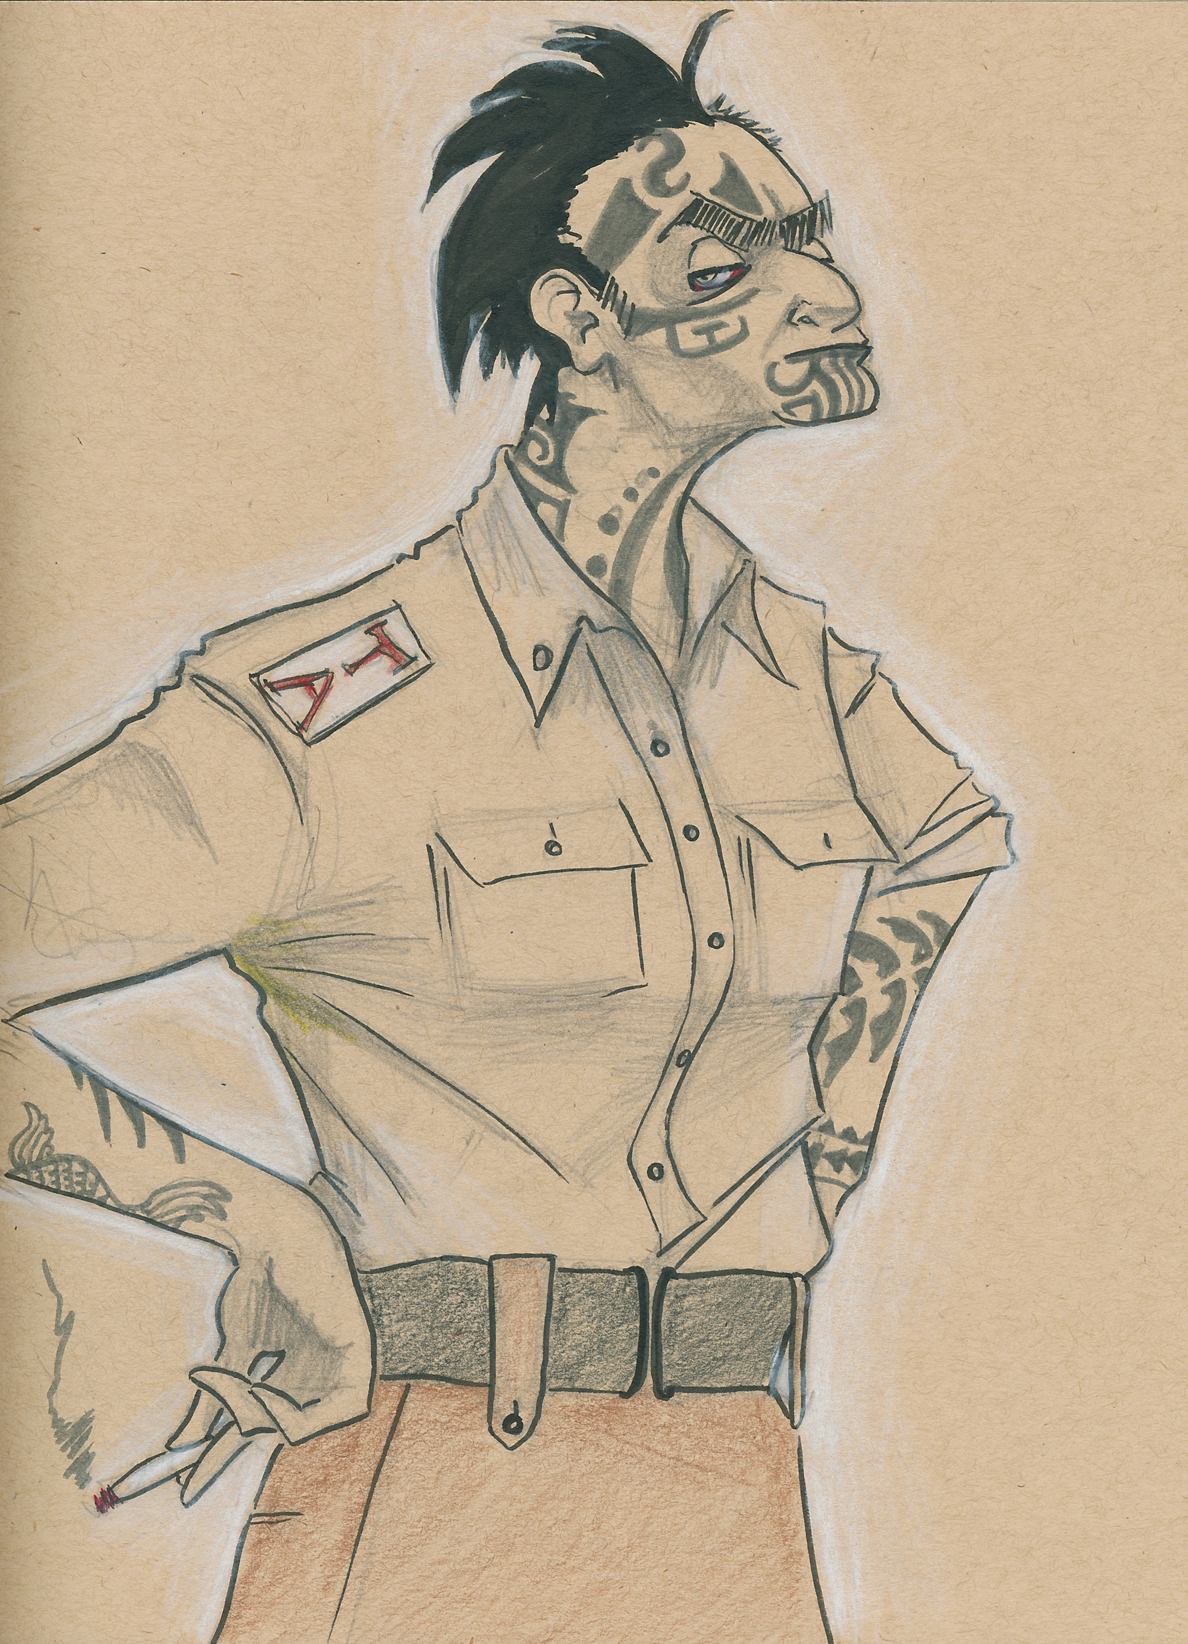
\includegraphics[width=12cm]{img/book1_jaya_misc_tough.png}
\end{center}
\newpage
~
   
\end{document}